\part{Atlas de los gráficos}

Esta parte recorre, página por página, todos los gráficos del sitio. Cada ficha reproduce la captura del gráfico y la explicación de su lupa: qué nos cuenta, cómo se lee, por qué importa, cómo interpretarlo, las fórmulas que producen las cifras y la metodología con su fuente oficial. Las capturas muestran los datos disponibles en la fecha de generación de este documento; en el sitio cada gráfico se actualiza solo.

\chapter{Ciclo}
\label{atlas:ciclo}

{\large\sffamily\bfseries El ciclo económico\par}\medskip

En qué fase está la economía, cómo llegó ahí y hacia dónde se mueve, trimestre a trimestre desde 2014.

{\small\color{cmmuted}Página del sitio: \url{https://stv-quant.github.io/ColombiaMacro-USBCali/ciclo/}}

\section{¿En qué parte del ciclo está la economía?}

\subsection{Reloj del ciclo: dónde estamos y hacia dónde vamos}
\label{g:g-ciclo-reloj}
\begin{center}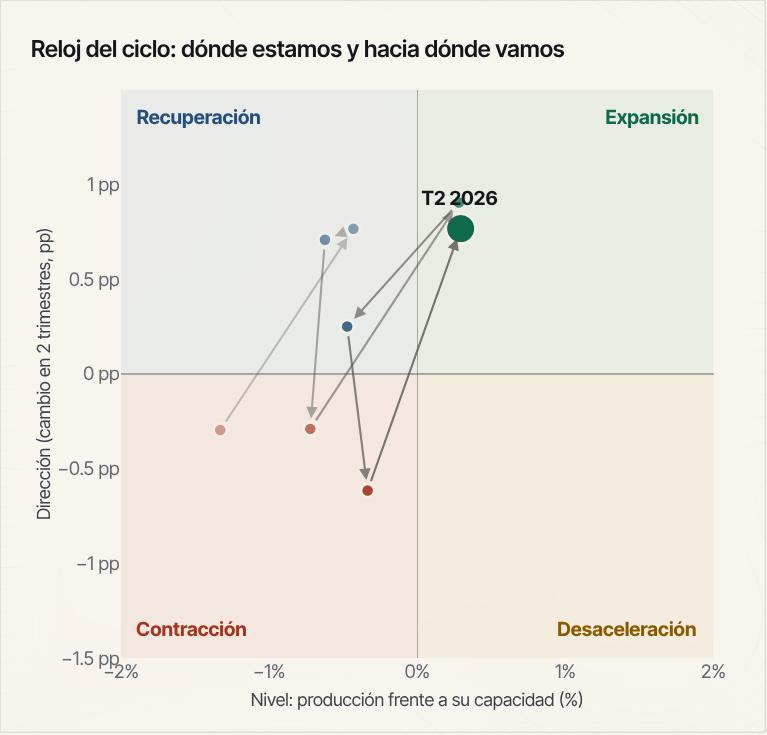
\includegraphics[width=\linewidth,height=0.42\textheight,keepaspectratio]{fig/g-ciclo-reloj.jpg}\end{center}
\paragraph{Qué nos cuenta}
El reloj del ciclo, una herramienta de la OCDE, ubica cada trimestre según dos preguntas: ¿la economía produce por encima o por debajo de su capacidad? y ¿esa distancia está aumentando o disminuyendo? La combinación define cuatro fases: expansión, desaceleración, contracción y recuperación.

\begin{leer}[Cómo se lee]
Eje horizontal: brecha del producto en porcentaje (a la derecha del cero, por encima de la capacidad). Eje vertical: cambio de la brecha en los últimos 2 trimestres, en puntos porcentuales (arriba, la brecha aumenta). Los cuadrantes llevan el color de su fase: verde expansión (arriba a la derecha), ámbar desaceleración (abajo a la derecha), rojo contracción (abajo a la izquierda) y azul recuperación (arriba a la izquierda). Cada punto es un trimestre, las flechas unen trimestres consecutivos y el punto grande es el elegido con el deslizador; los botones muestran la estela de 1, 2 o 3 años. Los ejes se ajustan al recorrido visible.
\end{leer}

\paragraph{Por qué importa}
No basta saber si la economía está por encima de su capacidad: importa hacia dónde se mueve. Una economía recalentada que pierde impulso (desaceleración) se lee de forma muy distinta a una que sigue acelerando (expansión). La fase es un marco común para interpretar inflación, tasas de interés y desempeño de los activos.

\paragraph{Cómo interpretarlo}
\begin{itemize}
\item Las economías tienden a recorrer el reloj en el sentido de las agujas: expansión $\rightarrow$ desaceleración $\rightarrow$ contracción $\rightarrow$ recuperación; pero el recorrido puede saltarse fases o retroceder.
\item Puntos cerca del centro indican una economía próxima a su capacidad y sin dirección clara: la fase en esos casos es frágil.
\item La dirección usa el cambio en 2 trimestres para reducir el ruido de un solo dato.
\item La brecha es la del filtro HP en tiempo real del gráfico de capacidad; otros métodos pueden ubicar el punto en otro cuadrante (vea el consenso de cinco métodos).
\end{itemize}
\begin{formulas}[Fórmulas]
\formula{Nivel (eje horizontal)}{brecha\textsubscript{t} = 100 $\times$ (ln Y\textsubscript{t} − ln Y*\textsubscript{t})}{Y = PIB real desestacionalizado; Y* = tendencia HP en tiempo real ($\lambda$ = 1.600)}
\formula{Dirección (eje vertical)}{$\Delta$\textsubscript{t} = brecha\textsubscript{t} − brecha\textsubscript{t−2}}{cambio en 2 trimestres, en pp}
\formula{Fase}{expansión: brecha $\ge$ 0 y $\Delta$ $\ge$ 0; desaceleración: brecha $\ge$ 0 y $\Delta$ < 0;\newline contracción: brecha < 0 y $\Delta$ < 0; recuperación: brecha < 0 y $\Delta$ $\ge$ 0}{cuadrante del reloj}
\end{formulas}
\begin{metodo}[Metodología]
Reloj del ciclo (metodología OCDE): eje horizontal = brecha del producto (HP en tiempo real); eje vertical = su cambio en 2 trimestres. La fase es el cuadrante.
\par\smallskip{\small\textbf{Fuente:} DANE, PIB real desestacionalizado; cálculo propio}
\end{metodo}

\subsection{Recorrido del ciclo trimestre a trimestre}
\label{g:g-ciclo-hist}
\begin{center}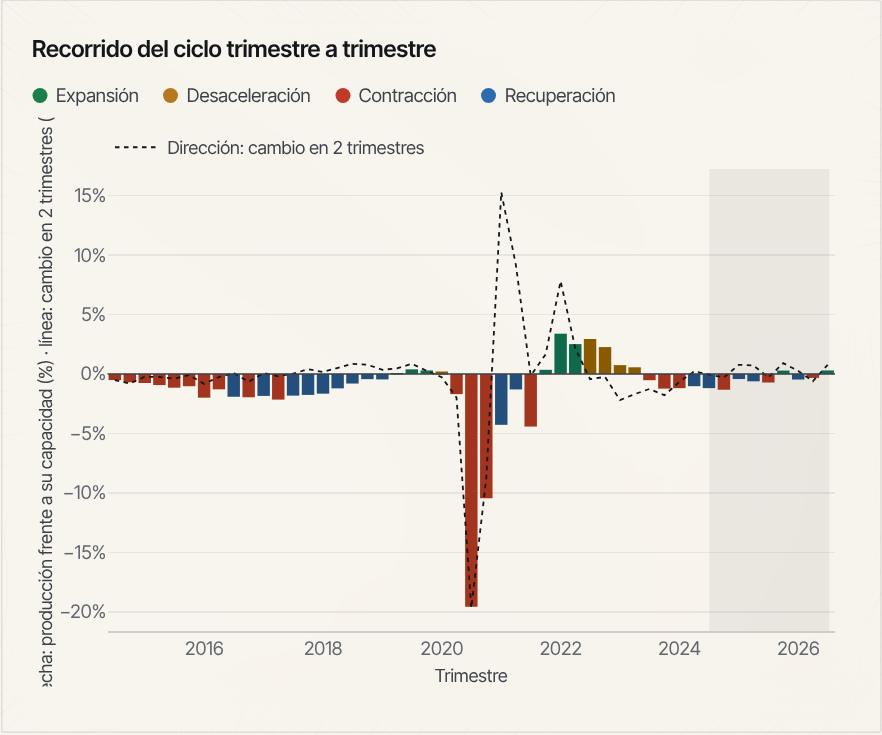
\includegraphics[width=\linewidth,height=0.42\textheight,keepaspectratio]{fig/g-ciclo-hist.jpg}\end{center}
\paragraph{Qué nos cuenta}
Es la historia completa del reloj del ciclo: la brecha del producto de cada trimestre, coloreada según la fase en que estaba la economía. Permite ver cuánto duran las fases, qué tan profundas son y cómo se suceden.

\begin{leer}[Cómo se lee]
Barras: brecha del producto (HP en tiempo real) en porcentaje, una por trimestre; el color indica la fase: verde expansión, ámbar desaceleración, rojo contracción y azul recuperación. Línea negra punteada: cambio de la brecha en 2 trimestres, en puntos porcentuales, que define la dirección. La franja gris sombrea los trimestres que se ven en el reloj; al mover el deslizador del reloj la franja se desplaza. La línea horizontal marca el cero.
\end{leer}

\paragraph{Por qué importa}
La secuencia de fases muestra si la economía viene de un período largo de holgura o de recalentamiento, contexto clave para leer la inflación y las decisiones de política monetaria. También permite comparar el momento actual con episodios anteriores, como el colapso de 2020 y su rebote.

\paragraph{Cómo interpretarlo}
\begin{itemize}
\item Barras verdes y ámbar arriba del cero: economía por encima de su capacidad; rojas y azules abajo: por debajo.
\item Cuando la línea punteada cruza el cero, la brecha cambia de dirección y la fase rota (por ejemplo, de expansión a desaceleración).
\item Cada barra usa solo la información disponible hasta ese trimestre (tiempo real), pero el PIB de los trimestres recientes puede revisarse.
\item La versión mensual con el ISE (Ciclo mensual) se actualiza antes y sirve para anticipar el dato trimestral.
\end{itemize}
\begin{formulas}[Fórmulas]
\formula{Brecha}{brecha\textsubscript{t} = 100 $\times$ (ln Y\textsubscript{t} − ln Y*\textsubscript{t})}{Y* = tendencia HP en tiempo real ($\lambda$ = 1.600), sin 2020T2–2021T2}
\formula{Dirección}{$\Delta$\textsubscript{t} = brecha\textsubscript{t} − brecha\textsubscript{t−2}}{línea punteada, en pp}
\end{formulas}
\begin{metodo}[Metodología]
Barras: brecha del producto por trimestre, coloreada por fase. Línea punteada: cambio de la brecha en 2 trimestres.
\par\smallskip{\small\textbf{Fuente:} DANE, PIB real desestacionalizado; cálculo propio}
\end{metodo}

\section{¿Qué tan seguros estamos de la fase?}

\subsection{Brecha del producto según cinco métodos (T2 2026)}
\label{g:g-consenso}
\begin{center}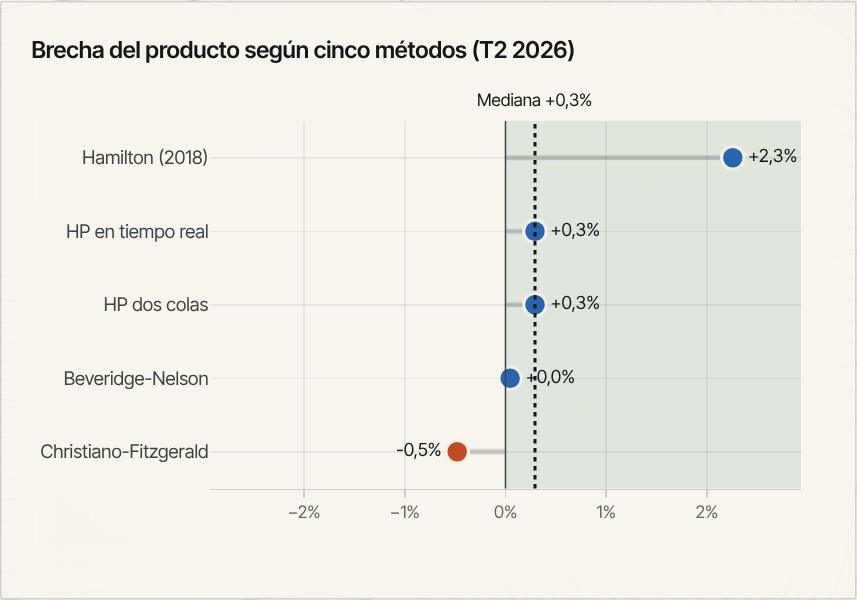
\includegraphics[width=\linewidth,height=0.42\textheight,keepaspectratio]{fig/g-consenso.jpg}\end{center}
\paragraph{Qué nos cuenta}
La brecha del producto no se observa: hay que estimarla, y cada método da una respuesta algo distinta. Este gráfico muestra la brecha del último trimestre según cinco métodos estándar de la literatura y su mediana, para separar lo que es una señal robusta de lo que depende del método elegido.

\begin{leer}[Cómo se lee]
Cada fila es un método y su punto marca la brecha en porcentaje, con el valor escrito al lado: azul si es positiva, naranja si es negativa; una varilla gris une el cero con cada punto. La zona sombreada en verde, a la derecha del cero, corresponde a producir por encima de la capacidad. La línea negra punteada vertical es la mediana de los cinco, con su valor arriba. Los métodos van ordenados de menor (abajo) a mayor brecha (arriba).
\end{leer}

\paragraph{Por qué importa}
Las decisiones basadas en una sola estimación de la brecha pueden ser frágiles. Cuando los cinco métodos coinciden en el signo, la lectura del ciclo es sólida; cuando se reparten a ambos lados del cero, la fase es incierta. Esto pesa en cómo se interpretan la inflación y la postura del Banco de la República.

\paragraph{Cómo interpretarlo}
\begin{itemize}
\item Puntos agrupados y del mismo lado del cero: lectura robusta. Puntos dispersos: incertidumbre alta; el rango (mínimo a máximo) mide esa incertidumbre.
\item El HP en tiempo real solo usa datos hasta cada trimestre; el HP de dos colas, Christiano-Fitzgerald y Beveridge-Nelson usan toda la muestra, por lo que su valor reciente cambia cuando llegan datos nuevos.
\item Hamilton compara el PIB con lo que anticipaba una regresión sobre su historia de hace 2 a 3 años; Beveridge-Nelson define el ciclo a partir del crecimiento esperado según un modelo autorregresivo.
\item En todos los métodos la tendencia se estima sin 2020T2–2021T2. Valores de la mediana entre −0,5\% y +0,5\% se leen como economía cerca de su potencial.
\end{itemize}
\begin{formulas}[Fórmulas]
\formula{Brecha (genérica)}{brecha\textsubscript{m,t} = 100 $\times$ ln Y\textsubscript{t} − $\tau$\textsubscript{m,t}}{Y = PIB real desestacionalizado; $\tau$\textsubscript{m} = tendencia (en 100 $\times$ log) según el método m}
\formula{Hamilton (2018)}{c\textsubscript{t} = y\textsubscript{t} − ($\beta$\textsubscript{0} + $\Sigma$\textsubscript{k=0..3} $\beta$\textsubscript{k+1} y\textsubscript{t−8−k})}{y = 100 $\times$ ln PIB; $\beta$ estimados por MCO (mínimos cuadrados ordinarios); horizonte 8 trimestres, 4 rezagos}
\formula{Christiano-Fitzgerald (2003)}{$\tau$\textsubscript{t} = y\textsubscript{t} − CF\textsubscript{6–32}(y)\textsubscript{t}}{CF = filtro de banda que aísla ciclos de 6 a 32 trimestres (1,5 a 8 años)}
\formula{Consenso}{mediana = med(brecha\textsubscript{1}, …, brecha\textsubscript{5}); rango = máx − mín}{los cinco métodos del gráfico}
\end{formulas}
\begin{metodo}[Metodología]
Cinco brechas del producto (log del PIB menos su tendencia): HP en tiempo real ($\lambda$ = 1.600, solo datos hasta cada trimestre); HP de dos colas; Hamilton (2018), error de proyección a 8 trimestres con 4 rezagos; Christiano y Fitzgerald (2003), filtro de banda de 6 a 32 trimestres; Beveridge y Nelson (1981) con un AR(4) del crecimiento. La tendencia se estima sin 2020T2–2021T2. La mediana es el consenso; el rango mide la incertidumbre.
\par\smallskip{\small\textbf{Fuente:} DANE, PIB real desestacionalizado; cálculo propio}
\end{metodo}

\subsection{Ciclo mensual: brecha del ISE}
\label{g:g-ciclo-mensual}
\begin{center}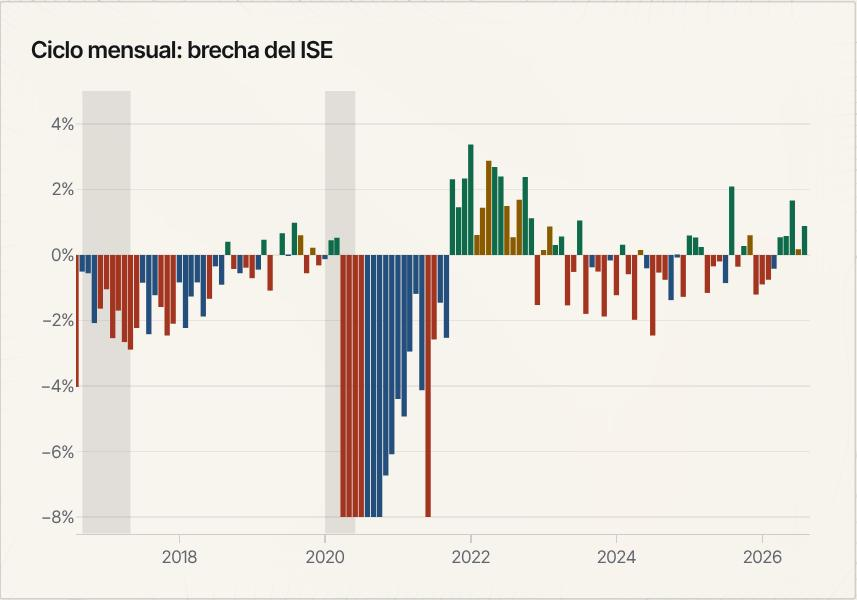
\includegraphics[width=\linewidth,height=0.42\textheight,keepaspectratio]{fig/g-ciclo-mensual.jpg}\end{center}
\paragraph{Qué nos cuenta}
Versión mensual de la brecha del producto, construida con el Indicador de Seguimiento a la Economía (ISE) del DANE, que mide la actividad económica cada mes y se publica unos 45 días antes que el PIB trimestral. Muestra cuánto se aleja la actividad de su tendencia y en qué fase del ciclo está cada mes.

\begin{leer}[Cómo se lee]
Cada barra es un mes: la brecha del ISE en porcentaje frente a su tendencia, coloreada por fase (verde expansión, ámbar desaceleración, rojo contracción, azul recuperación). Las franjas grises sombrean las recesiones fechadas en la tabla de expansiones y recesiones. Los meses de 2020 con brechas menores a −8\% se recortan en ese valor para que no aplasten la escala; el valor real aparece al pasar el cursor.
\end{leer}

\paragraph{Por qué importa}
Al llegar antes que el PIB, la brecha mensual da una lectura temprana del ciclo y permite detectar giros con menos rezago. Es útil para seguir la economía entre publicaciones trimestrales y para contrastar la fase que muestra el reloj del ciclo.

\paragraph{Cómo interpretarlo}
\begin{itemize}
\item Barras positivas: actividad por encima de su tendencia; negativas: por debajo. El color indica además si la brecha sube o baja frente a 3 meses antes.
\item Una racha de varios meses del mismo color es más informativa que un mes aislado: el ISE es volátil y se revisa.
\item La tendencia es un HP en tiempo real con $\lambda$ = 129.600, el equivalente mensual del $\lambda$ = 1.600 trimestral (Ravn y Uhlig), y excluye marzo de 2020 a junio de 2021.
\item Las recesiones sombreadas son caídas del nivel del ISE, un concepto distinto de la brecha negativa: puede haber brecha negativa sin recesión.
\end{itemize}
\begin{formulas}[Fórmulas]
\formula{Brecha mensual}{b\textsubscript{t} = 100 $\times$ ln ISE\textsubscript{t} − $\tau$\textsubscript{t}}{ISE desestacionalizado; $\tau$ = tendencia HP en tiempo real de 100 $\times$ ln ISE ($\lambda$ = 129.600, solo datos hasta t)}
\formula{Dirección}{$\Delta$\textsubscript{t} = b\textsubscript{t} − b\textsubscript{t−3}}{cambio en 3 meses; la fase combina el signo de b y de $\Delta$}
\end{formulas}
\begin{metodo}[Metodología]
Brecha = 100 $\times$ (log ISE − tendencia HP en tiempo real, $\lambda$ = 129.600 de Ravn y Uhlig). La tendencia excluye mar-2020 a jun-2021. Fase: signo de la brecha y su cambio en 3 meses (reloj del ciclo de la OCDE).
\par\smallskip{\small\textbf{Fuente:} DANE, Indicador de Seguimiento a la Economía (ISE), serie desestacionalizada}
\end{metodo}

\section{¿Qué mueve el ciclo?}

\subsection{Las tres grandes ramas frente a su tendencia (jul 2026)}
\label{g:g-motores}
\begin{center}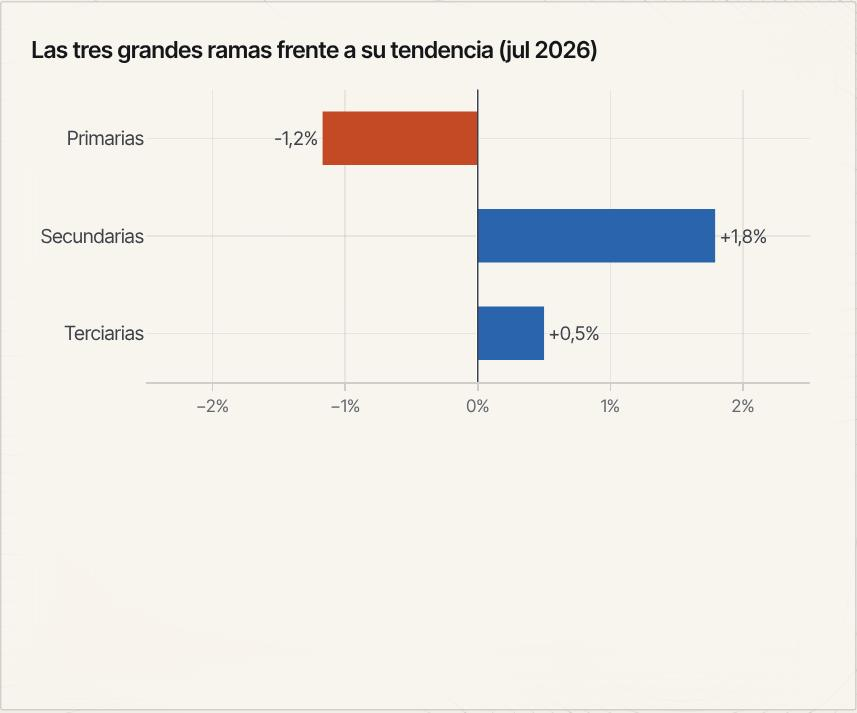
\includegraphics[width=\linewidth,height=0.42\textheight,keepaspectratio]{fig/g-motores.jpg}\end{center}
\paragraph{Qué nos cuenta}
Descompone la brecha mensual del ISE en las tres grandes ramas de la economía: actividades primarias (agro y minería), secundarias (industria, construcción y servicios públicos) y terciarias (comercio, servicios y Gobierno). Muestra qué parte de la economía está por encima o por debajo de su propia tendencia en el último mes publicado.

\begin{leer}[Cómo se lee]
Tres barras horizontales, una por rama, con la brecha en porcentaje y su valor escrito al final. Azul: la rama produce por encima de su tendencia; naranja: por debajo. La línea vertical marca el cero y el eje es simétrico. Al pasar el cursor también se ve el crecimiento anual de cada rama frente al mismo mes del año anterior.
\end{leer}

\paragraph{Por qué importa}
Las ramas responden a fuerzas distintas: las primarias, a precios internacionales, clima y producción petrolera; las secundarias, a la inversión y la construcción; las terciarias, al consumo de los hogares y el gasto público. Saber cuál empuja o frena el ciclo ayuda a entender su naturaleza y su sensibilidad a tasas de interés o a choques externos.

\paragraph{Cómo interpretarlo}
\begin{itemize}
\item Las terciarias son la mayor parte de la economía, así que su brecha pesa más en la brecha total del ISE.
\item Una rama puede crecer frente al año anterior y aun así estar por debajo de su tendencia (y al revés): brecha y crecimiento anual miden cosas distintas.
\item Las primarias son las más volátiles mes a mes; conviene mirar varios meses antes de sacar conclusiones.
\item Para el detalle por sector (12 ramas, trimestral) vea los aportes al crecimiento y la amplitud sectorial.
\end{itemize}
\begin{formulas}[Fórmulas]
\formula{Brecha por rama}{b\textsubscript{r,t} = 100 $\times$ ln X\textsubscript{r,t} − $\tau$\textsubscript{r,t}}{X = ISE desestacionalizado de la rama r; $\tau$ = tendencia HP en tiempo real ($\lambda$ = 129.600), sin mar-2020 a jun-2021}
\formula{Crecimiento anual (en el cursor)}{g\textsubscript{r,t} = (X\textsubscript{r,t} $\div$ X\textsubscript{r,t−12} − 1) $\times$ 100}{mismo mes del año anterior}
\end{formulas}
\begin{metodo}[Metodología]
Misma brecha mensual del ISE, calculada para actividades primarias, secundarias y terciarias por separado.
\par\smallskip{\small\textbf{Fuente:} DANE, ISE por grandes ramas, series desestacionalizadas}
\end{metodo}

\subsection{¿Quién aporta el crecimiento? Puntos del PIB por sector (T2 2026)}
\label{g:g-aportes}
\begin{center}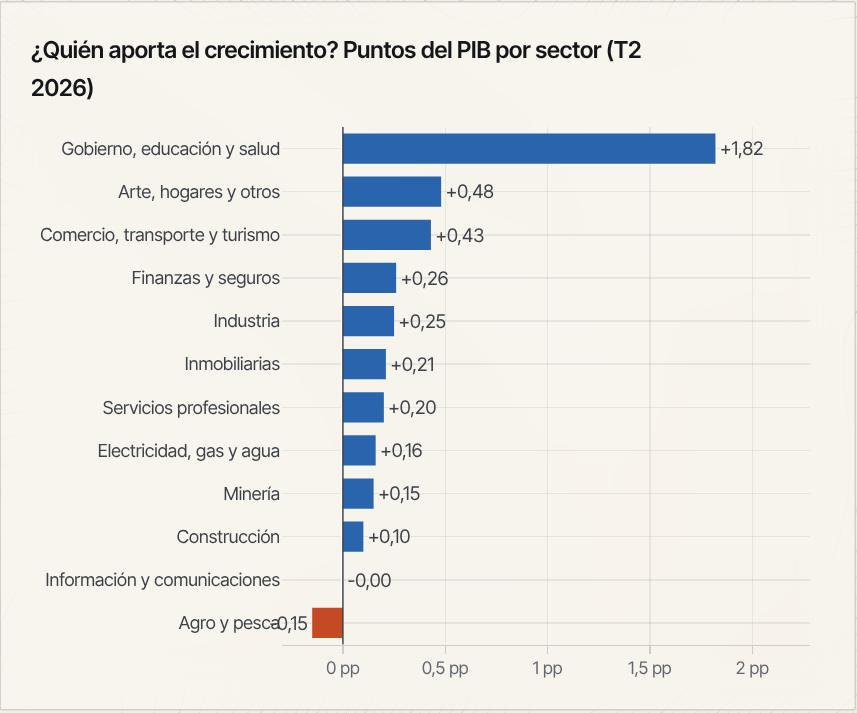
\includegraphics[width=\linewidth,height=0.42\textheight,keepaspectratio]{fig/g-aportes.jpg}\end{center}
\paragraph{Qué nos cuenta}
Reparte el crecimiento anual de la economía entre las 12 grandes ramas de actividad: cuántos puntos porcentuales suma o resta cada sector en el último trimestre publicado. Responde a la pregunta de quién está generando el crecimiento.

\begin{leer}[Cómo se lee]
Barras horizontales, una por sector, con su aporte en puntos porcentuales (pp) y el valor escrito al final; azul si suma, naranja si resta. La línea vertical marca el cero y los sectores van ordenados del mayor aporte (arriba) al menor (abajo). Al pasar el cursor se ve también el crecimiento anual del sector. La suma de las barras se aproxima al crecimiento anual del valor agregado.
\end{leer}

\paragraph{Por qué importa}
Un mismo crecimiento total puede venir de sectores muy distintos: no es igual que lo impulse la agricultura que la construcción o los servicios financieros. El aporte combina el ritmo del sector con su tamaño, por lo que muestra qué actividades sostienen realmente la expansión y qué tan concentrada está.

\paragraph{Cómo interpretarlo}
\begin{itemize}
\item Un sector pequeño con crecimiento alto puede aportar menos que uno grande con crecimiento moderado; el aporte refleja ambos.
\item Si pocos sectores explican casi todo el crecimiento, la expansión depende de pocas fuentes; compárelo con la amplitud sectorial.
\item Los datos son originales (sin desestacionalizar) y comparan con el mismo trimestre del año anterior, lo que neutraliza la estacionalidad, pero no los efectos de calendario (como la Semana Santa) ni las bases de comparación atípicas.
\item Como los volúmenes encadenados no son aditivos, la suma de aportes difiere levemente del crecimiento total publicado por el DANE; el peso usado es el del valor agregado, no el del PIB con impuestos.
\end{itemize}
\begin{formulas}[Fórmulas]
\formula{Aporte del sector}{a\textsubscript{i,t} = (X\textsubscript{i,t} − X\textsubscript{i,t−4}) $\div$ VA\textsubscript{t−4} $\times$ 100}{X = valor agregado real del sector i; VA = valor agregado real total; t−4 = mismo trimestre del año anterior}
\formula{Forma equivalente}{a\textsubscript{i,t} = g\textsubscript{i,t} $\times$ w\textsubscript{i,t−4}}{g = crecimiento anual del sector (\%); w = peso del sector en el valor agregado un año antes (tanto por uno)}
\formula{Suma}{$\Sigma$\textsubscript{i} a\textsubscript{i,t} $\approx$ crecimiento anual del valor agregado}{aproximación por la no aditividad de los encadenados}
\end{formulas}
\begin{metodo}[Metodología]
Aporte = crecimiento anual real del sector $\times$ su peso en el PIB del mismo trimestre del año anterior (precios constantes). La suma de los aportes es el crecimiento del PIB a precios básicos.
\par\smallskip{\small\textbf{Fuente:} DANE, PIB trimestral (anexos de producción a precios constantes y corrientes)}
\end{metodo}

\subsection{¿Cuántos sectores están por encima de su tendencia? (T2 2026)}
\label{g:v-amplitud-sectores}
\begin{center}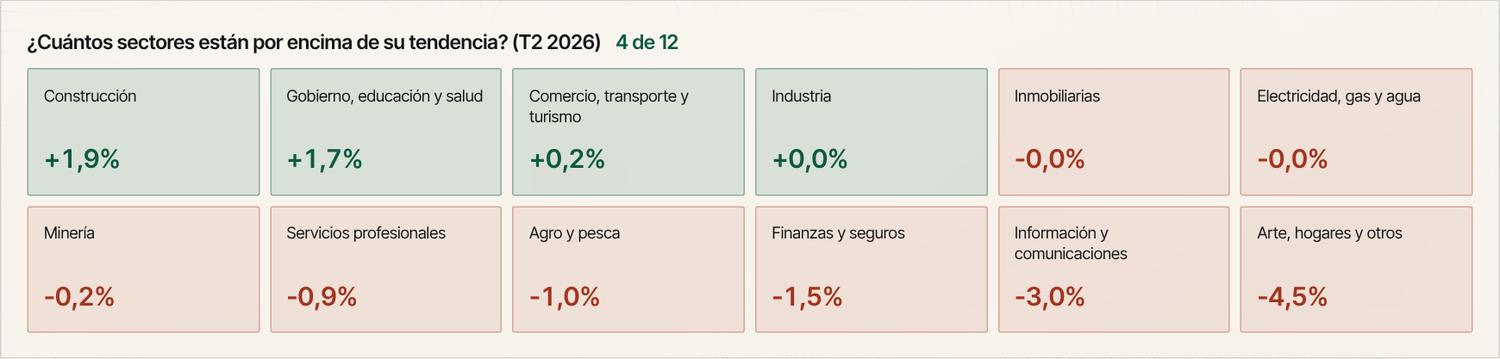
\includegraphics[width=\linewidth,height=0.42\textheight,keepaspectratio]{fig/v-amplitud-sectores.jpg}\end{center}
\paragraph{Qué nos cuenta}
Cuenta cuántos de los 12 grandes sectores de la economía producen por encima de su propia tendencia en el último trimestre. Es un índice de difusión: mide si la expansión es amplia, con la mayoría de los sectores participando, o estrecha, concentrada en unos pocos.

\begin{leer}[Cómo se lee]
Una casilla por sector, ordenadas de mayor a menor brecha, con el nombre y la brecha en porcentaje. Verde: el sector está por encima de su tendencia; rojo-naranja: por debajo. Junto al título se indica cuántos de los 12 están en verde. Más de 6 sectores en verde se considera una expansión generalizada.
\end{leer}

\paragraph{Por qué importa}
Una expansión amplia suele ser más sólida y generar presiones de precios más extendidas; una estrecha depende de pocos motores y es más vulnerable a que alguno se frene. La amplitud complementa a la brecha agregada, que puede ser positiva aunque la mayoría de sectores tenga holgura.

\paragraph{Cómo interpretarlo}
\begin{itemize}
\item 7 o más casillas verdes: expansión generalizada; 6 o menos: expansión concentrada.
\item La brecha de cada sector se mide frente a su propia tendencia, calculada con la suma de 4 trimestres de su valor agregado real (datos originales) y un filtro HP en tiempo real.
\item Las casillas son la misma información que el gráfico de barras «Brecha de cada sector hoy» de la página Capacidad.
\item Un sector justo por encima o por debajo de cero puede cambiar de color con revisiones pequeñas del DANE.
\end{itemize}
\begin{formulas}[Fórmulas]
\formula{Brecha sectorial}{b\textsubscript{i,t} = 100 $\times$ (ln N\textsubscript{i,t} − ln T\textsubscript{i,t})}{N = suma de 4 trimestres del valor agregado real del sector i; T = tendencia HP en tiempo real ($\lambda$ = 1.600), sin 2020T2–2021T2}
\formula{Amplitud}{A\textsubscript{t} = $\Sigma$\textsubscript{i=1..12} 1[b\textsubscript{i,t} > 0]}{1[$\cdot$] vale 1 si el sector está sobre su tendencia y 0 si no}
\end{formulas}

\section{¿Qué tan fuerte y qué tan larga es esta expansión?}

\subsection{Ritmo de la actividad: anual frente a los últimos 3 meses}
\label{g:g-ritmo}
\begin{center}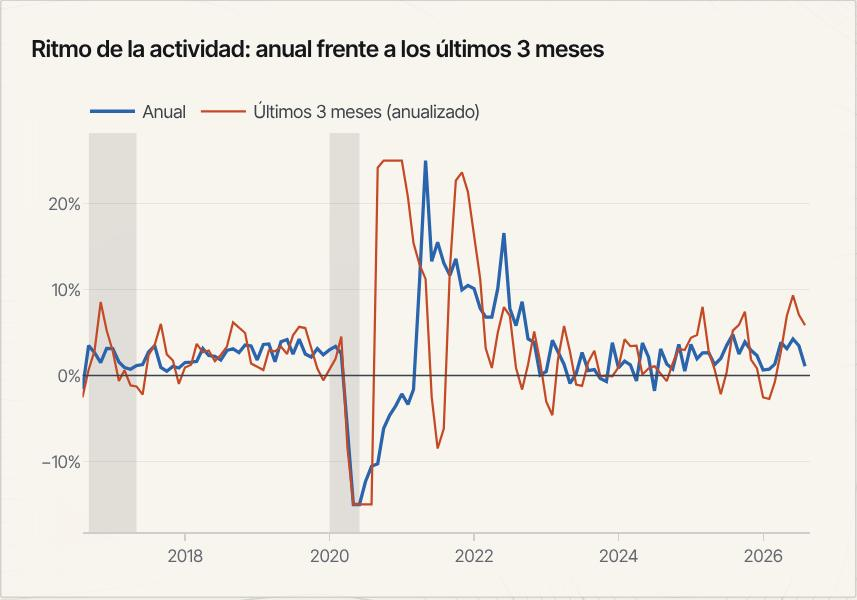
\includegraphics[width=\linewidth,height=0.42\textheight,keepaspectratio]{fig/g-ritmo.jpg}\end{center}
\paragraph{Qué nos cuenta}
Compara dos velocidades de la actividad económica medida con el ISE: el crecimiento anual, que mira 12 meses hacia atrás, y el ritmo de los últimos tres meses, que capta el impulso más reciente. Cuando ambas difieren, la economía está cambiando de marcha.

\begin{leer}[Cómo se lee]
Línea azul: variación del ISE desestacionalizado frente al mismo mes del año anterior, en porcentaje. Línea naranja, más delgada: promedio de los últimos 3 meses frente a los 3 anteriores, llevado a tasa anual. Las franjas grises son recesiones y la línea horizontal marca el cero. Ambas series se recortan entre −15\% y 25\% para que los extremos de 2020 y su rebote no aplasten la escala.
\end{leer}

\paragraph{Por qué importa}
El crecimiento anual es estable pero lento para reflejar giros; el ritmo de 3 meses los muestra antes, a costa de más ruido. Leerlos juntos ayuda a distinguir una economía que acelera de una que se modera, información relevante para la lectura de la inflación, las tasas y las utilidades empresariales.

\paragraph{Cómo interpretarlo}
\begin{itemize}
\item Naranja por encima de azul: el impulso reciente supera al promedio del año (aceleración); por debajo: moderación.
\item Naranja por debajo de cero con azul aún positivo: la actividad ya cae en el margen aunque la comparación anual siga favorable.
\item Anualizar multiplica el ruido mensual por cuatro: un solo dato atípico o una revisión puede mover mucho la línea naranja.
\item La comparación anual hereda efectos de base: un año anterior muy débil o muy fuerte infla o reduce la variación sin reflejar el momento actual.
\end{itemize}
\begin{formulas}[Fórmulas]
\formula{Crecimiento anual}{g\textsubscript{t} = (ISE\textsubscript{t} $\div$ ISE\textsubscript{t−12} − 1) $\times$ 100}{ISE desestacionalizado del mes t}
\formula{Ritmo de 3 meses anualizado}{r\textsubscript{t} = [(M3\textsubscript{t} $\div$ M3\textsubscript{t−3})\textsuperscript{4} − 1] $\times$ 100}{M3\textsubscript{t} = promedio del ISE desestacionalizado en t, t−1 y t−2}
\end{formulas}
\begin{metodo}[Metodología]
Anual: variación frente al mismo mes del año anterior. Últimos 3 meses: (promedio de los 3 últimos / promedio de los 3 anteriores)\textasciicircum{}4 − 1. Ambas se recortan en −15\% y 25\% para que 2020 no aplaste la escala.
\par\smallskip{\small\textbf{Fuente:} DANE, ISE desestacionalizado}
\end{metodo}

\subsection{Expansiones y recesiones desde 2008}
\label{g:v-fases-ciclo}
\begin{center}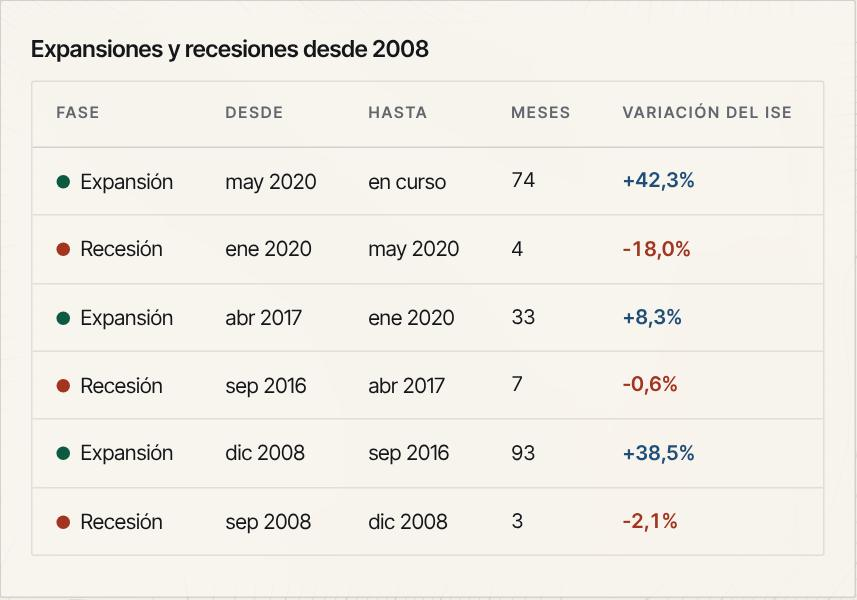
\includegraphics[width=\linewidth,height=0.42\textheight,keepaspectratio]{fig/v-fases-ciclo.jpg}\end{center}
\paragraph{Qué nos cuenta}
Fecha las expansiones y recesiones de la economía colombiana a partir del nivel del ISE: una recesión va de un pico a un valle de la actividad y una expansión de un valle al siguiente pico. Es el «ciclo clásico», basado en caídas absolutas de la producción, distinto del ciclo de brechas del reloj.

\begin{leer}[Cómo se lee]
Tabla con una fila por fase, de la más reciente arriba a la más antigua abajo. Columnas: tipo de fase (punto verde expansión, rojo recesión), mes de inicio, mes de fin («en curso» si no ha terminado), duración en meses y variación porcentual del ISE entre el inicio y el fin de la fase (verde si sube, rojo si baja). Las recesiones de esta tabla son las franjas grises de los gráficos mensuales del sitio.
\end{leer}

\paragraph{Por qué importa}
La duración y la profundidad de recesiones y expansiones pasadas son la vara para medir el ciclo actual: cuánto lleva la expansión en curso y cuánto ha crecido la actividad desde el último valle. Colombia no tiene un comité oficial de fechado del ciclo, por lo que este fechado académico ofrece una referencia sistemática.

\paragraph{Cómo interpretarlo}
\begin{itemize}
\item Picos y valles son máximos y mínimos locales del promedio móvil centrado de 3 meses del ISE desestacionalizado, dentro de ventanas de $\pm$6 meses, y se fuerzan a alternarse (método en la línea de Bry y Boschan, 1971).
\item Por construcción, un giro solo puede confirmarse cuando hay al menos 7 meses de datos posteriores: la última fase puede figurar «en curso» aunque la actividad ya haya girado.
\item La variación de una fase en curso se mide hasta el último promedio centrado disponible y cambia con cada dato y con las revisiones del ISE.
\item Es un fechado estadístico, no oficial; recesiones muy cortas o suaves pueden no detectarse o fecharse distinto con otras reglas.
\end{itemize}
\begin{formulas}[Fórmulas]
\formula{Serie suavizada}{S\textsubscript{t} = (ISE\textsubscript{t−1} + ISE\textsubscript{t} + ISE\textsubscript{t+1}) $\div$ 3}{ISE desestacionalizado; promedio móvil centrado de 3 meses}
\formula{Pico (valle)}{S\textsubscript{t} = máx (mín) \{S\textsubscript{t−6}, …, S\textsubscript{t+6}\}}{extremo local en una ventana de $\pm$6 meses; picos y valles alternados}
\formula{Variación de la fase}{v = (S\textsubscript{fin} $\div$ S\textsubscript{inicio} − 1) $\times$ 100}{S en el giro final (o el último disponible si la fase sigue en curso) frente al giro inicial}
\end{formulas}

\section{¿Cómo se refleja el ciclo en el empleo?}

\subsection{Cambio en 12 meses: desempleo y ocupación}
\label{g:g-empleo-ciclo}
\begin{center}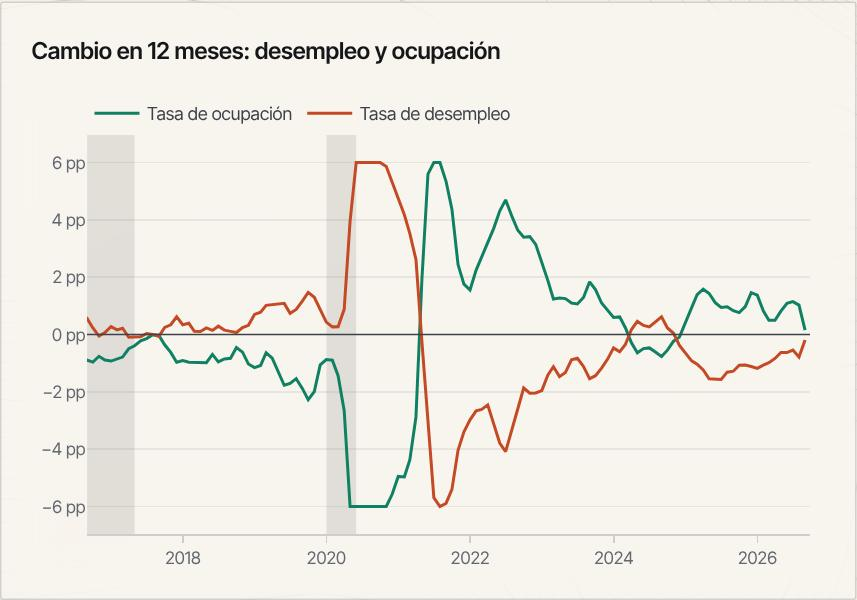
\includegraphics[width=\linewidth,height=0.42\textheight,keepaspectratio]{fig/g-empleo-ciclo.jpg}\end{center}
\paragraph{Qué nos cuenta}
Muestra cómo se transmite el ciclo al mercado laboral: el cambio en 12 meses de la tasa de desempleo y de la tasa de ocupación. Permite ver si la actividad económica se está traduciendo en más empleo o si el mercado laboral se debilita.

\begin{leer}[Cómo se lee]
Dos líneas mensuales en puntos porcentuales (pp): verde, cambio de la tasa de ocupación; naranja, cambio de la tasa de desempleo. Cada punto compara el promedio de los últimos 3 meses de la tasa desestacionalizada con el mismo promedio un año antes. La línea horizontal marca el cero, las franjas grises son recesiones y los valores se recortan en $\pm$6 pp para que el choque de 2020 no aplaste la escala.
\end{leer}

\paragraph{Por qué importa}
El empleo es el canal por el que el ciclo llega a los hogares: sostiene el consumo y la confianza. Un mercado laboral que mejora refuerza la demanda interna; uno que se deteriora la debilita. Además, la presión salarial que genera un mercado laboral apretado es un insumo clave para la inflación y la política monetaria.

\paragraph{Cómo interpretarlo}
\begin{itemize}
\item Verde por encima de cero y naranja por debajo: mercado laboral que mejora (más ocupados, menos desempleo). Lo contrario indica deterioro.
\item El desempleo puede bajar sin que suba la ocupación si menos personas buscan trabajo; por eso conviene mirar las dos líneas juntas.
\item Promediar 3 meses reduce el ruido de la encuesta (GEIH), pero los cambios se reflejan con algo de rezago.
\item En Colombia el empleo responde poco al ciclo (vea la ley de Okun), en parte porque la informalidad absorbe los choques.
\end{itemize}
\begin{formulas}[Fórmulas]
\formula{Promedio de 3 meses}{$\bar{x}$\textsubscript{t} = (x\textsubscript{t} + x\textsubscript{t−1} + x\textsubscript{t−2}) $\div$ 3}{x = tasa de desempleo o de ocupación desestacionalizada}
\formula{Cambio en 12 meses}{$\Delta$\textsubscript{12}$\bar{x}$\textsubscript{t} = $\bar{x}$\textsubscript{t} − $\bar{x}$\textsubscript{t−12}}{en puntos porcentuales}
\formula{Tasas}{TD = D $\div$ FT $\times$ 100; TO = O $\div$ PET $\times$ 100}{D = desocupados; O = ocupados; FT = fuerza de trabajo; PET = población en edad de trabajar}
\end{formulas}
\begin{metodo}[Metodología]
Diferencia en puntos porcentuales entre el promedio de 3 meses de cada tasa (desestacionalizada) y el mismo promedio 12 meses antes.
\par\smallskip{\small\textbf{Fuente:} DANE, Gran Encuesta Integrada de Hogares (GEIH)}
\end{metodo}

\subsection{Ley de Okun: producción y empleo se mueven juntos, pero poco}
\label{g:g-okun}
\begin{center}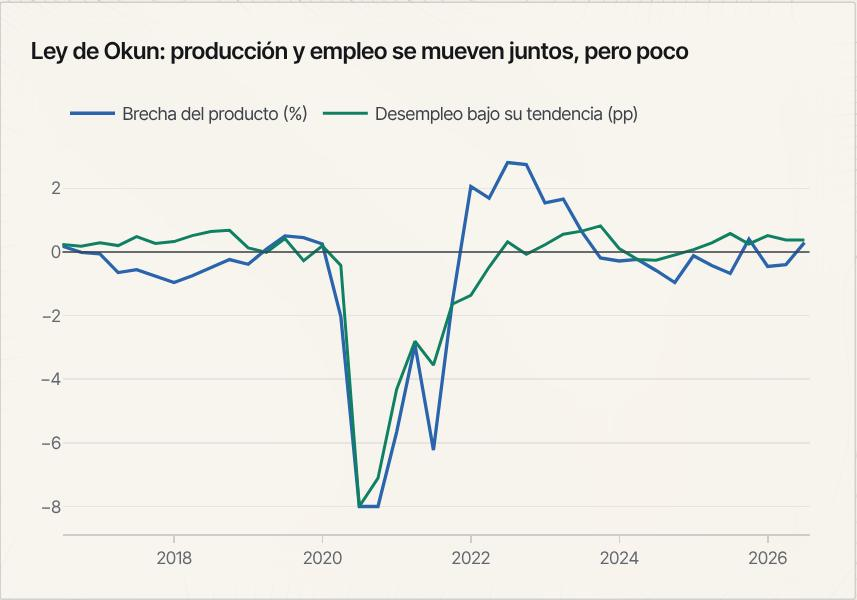
\includegraphics[width=\linewidth,height=0.42\textheight,keepaspectratio]{fig/g-okun.jpg}\end{center}
\paragraph{Qué nos cuenta}
Pone a prueba la ley de Okun, la regularidad según la cual cuando la economía produce por encima de su capacidad el desempleo cae por debajo de su nivel de tendencia. Compara la brecha del producto con la brecha de desempleo para ver cuánto se mueven juntas en Colombia.

\begin{leer}[Cómo se lee]
Dos líneas trimestrales: azul, brecha del producto en porcentaje (filtro HP de dos colas); verde, cuánto está el desempleo por debajo de su tendencia, en puntos porcentuales. La verde está invertida (desempleo bajo la tendencia = valor positivo) para que ambas suban juntas en una economía recalentada. La línea horizontal marca el cero y ambas se recortan en $\pm$8 para que 2020 no aplaste la escala.
\end{leer}

\paragraph{Por qué importa}
La fuerza de la relación indica cuánto empleo genera un punto adicional de actividad. Si es débil, el crecimiento se traduce poco en empleo formal y la holgura laboral puede persistir aunque la economía crezca, lo que afecta la lectura de presiones salariales e inflación y el diagnóstico del Banco de la República.

\paragraph{Cómo interpretarlo}
\begin{itemize}
\item Líneas que suben y bajan juntas confirman la relación; si se separan, el empleo no está acompañando a la producción.
\item La pendiente $\beta$ se estima por mínimos cuadrados ordinarios (MCO) con todos los trimestres disponibles excepto 2020–2021; una $\beta$ cercana a cero indica que el desempleo responde poco a la producción. Su valor y la correlación se muestran en el texto de la sección.
\item En Colombia la relación es débil, en parte porque la informalidad absorbe los choques: en las recesiones muchas personas pasan a empleos informales en lugar de al desempleo.
\item Ambas tendencias usan filtros HP de dos colas, que se reestiman con cada dato nuevo: los valores recientes de las dos brechas pueden cambiar.
\end{itemize}
\begin{formulas}[Fórmulas]
\formula{Brecha de desempleo}{b\textsuperscript{u}\textsubscript{t} = u\textsubscript{t} − u*\textsubscript{t}}{u = promedio trimestral del desempleo desestacionalizado; u* = tendencia HP de dos colas ($\lambda$ = 1.600), sin 2020T2–2021T2}
\formula{Línea verde}{−b\textsuperscript{u}\textsubscript{t}}{positiva cuando el desempleo está por debajo de su tendencia}
\formula{Ley de Okun en brechas}{b\textsuperscript{u}\textsubscript{t} = $\alpha$ + $\beta$ $\times$ brecha\textsubscript{t} + $\varepsilon$\textsubscript{t}}{brecha = brecha del producto (HP dos colas); $\beta$ < 0 esperado; estimado por MCO sin 2020–2021}
\end{formulas}
\begin{metodo}[Metodología]
Okun (1962) en brechas: (desempleo − tendencia HP) = $\beta$ $\times$ brecha del producto (HP dos colas). Se estima por MCO con 2009–2025 sin 2020–2021. Una $\beta$ cercana a cero indica que el empleo responde poco a la producción.
\par\smallskip{\small\textbf{Fuente:} DANE: PIB real y GEIH; cálculo propio}
\end{metodo}

\chapter{Crecimiento}
\label{atlas:crecimiento}

{\large\sffamily\bfseries Crecimiento, sectores y demanda\par}\medskip

Cuánto crece la economía y por qué: por la oferta (los 12 sectores del PIB) y por la demanda (hogares, Gobierno, inversión y comercio exterior), con el PIB por persona y la productividad.

{\small\color{cmmuted}Página del sitio: \url{https://stv-quant.github.io/ColombiaMacro-USBCali/crecimiento/}}

\section{¿Está creciendo la economía?}

\subsection{Crecimiento anual de la economía}
\label{g:g-crec}
\begin{center}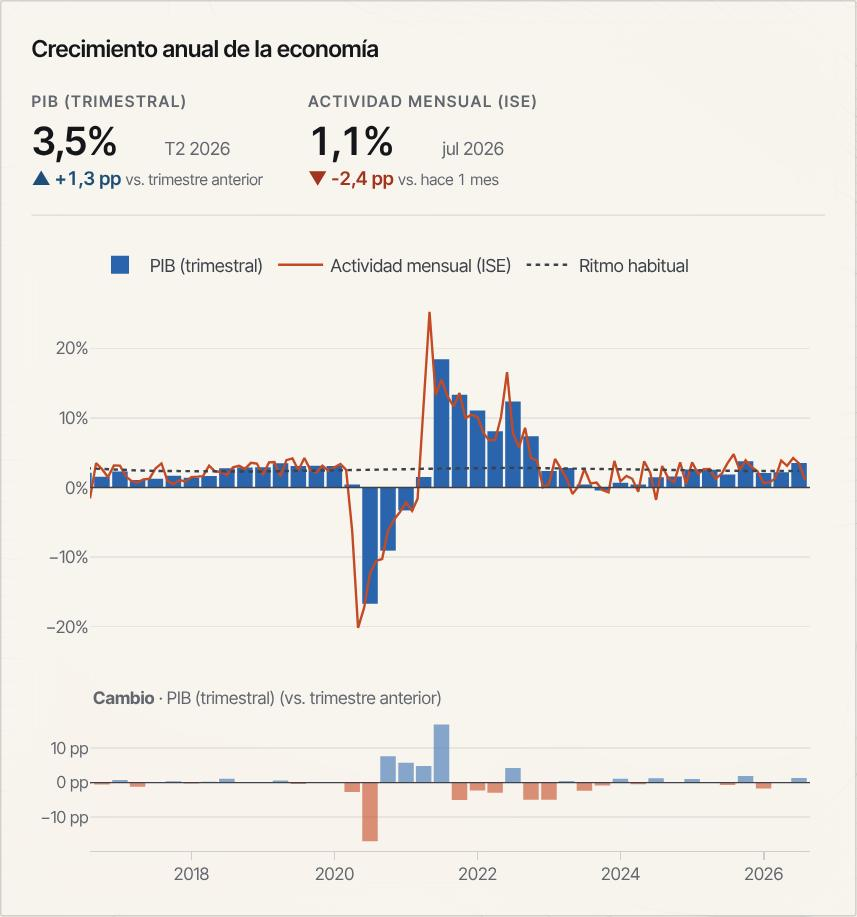
\includegraphics[width=\linewidth,height=0.42\textheight,keepaspectratio]{fig/g-crec.jpg}\end{center}
\paragraph{Qué nos cuenta}
Muestra a qué ritmo crece la producción de bienes y servicios de Colombia frente al mismo trimestre del año anterior y lo compara con el ritmo habitual de la economía. Junto al PIB trimestral aparece el Indicador de Seguimiento a la Economía (ISE), un índice mensual del DANE que resume la actividad de todos los sectores y llega antes que el PIB. En conjunto cuentan la historia del ciclo: periodos en que la economía corre por encima de su ritmo normal y periodos en que se queda por debajo, como el desplome de 2020 y el rebote que le siguió.

\begin{leer}[Cómo se lee]
Panel superior, eje en \%: las barras azules son la variación anual del PIB real de cada trimestre (datos originales, sin desestacionalizar); la línea naranja es la variación anual del ISE desestacionalizado, mes a mes; la línea gris punteada es el «ritmo habitual», el crecimiento anual de la tendencia estimada con el filtro de Hodrick-Prescott (HP). La línea horizontal en cero separa crecimiento de contracción. El panel inferior muestra, en puntos porcentuales (pp), cuánto cambió la tasa anual del PIB frente al trimestre anterior: azul si subió, naranja si bajó. La vista inicial cubre los últimos diez años; el resto de la historia se ve ampliando el eje.
\end{leer}

\paragraph{Por qué importa}
El crecimiento del PIB resume en una cifra la evolución de los ingresos, el empleo y las ventas de las empresas. Compararlo con el ritmo habitual indica si la economía genera presiones de demanda sobre su capacidad o si tiene holgura, una distinción central para leer la inflación y las decisiones de tasas del Banco de la República. Para un inversionista es el punto de partida para evaluar utilidades corporativas, recaudo tributario y calidad del crédito.

\paragraph{Cómo interpretarlo}
\begin{itemize}
\item Barras por encima de la línea punteada: la economía crece más rápido que su tendencia; por debajo, más despacio. Barras negativas indican que se produce menos que un año antes.
\item El panel inferior muestra la dirección: varias barras azules seguidas indican aceleración y varias naranjas, desaceleración, aunque el crecimiento siga siendo positivo.
\item El ISE cubre meses que el PIB trimestral aún no recoge: si la línea naranja se separa de la última barra, la actividad reciente se movió en esa dirección. La brecha frente al ritmo habitual se estudia en la página de capacidad.
\item Los datos originales incluyen efectos de calendario (Semana Santa, días hábiles) y efectos base: tras una caída fuerte, la tasa anual sube mucho aunque el nivel apenas se recupere, como en 2021.
\item La tendencia HP se reestima con cada dato nuevo y su tramo final es el menos preciso; los trimestres 2020T2–2021T2 se reemplazan por interpolación al estimarla. El DANE revisa el PIB en cada publicación.
\end{itemize}
\begin{formulas}[Fórmulas]
\formula{Variación anual del PIB}{g\textsubscript{t} = (Y\textsubscript{t} $\div$ Y\textsubscript{t−4} − 1) $\times$ 100}{Y\textsubscript{t} = PIB real del trimestre t (volúmenes encadenados, base 2015, datos originales)}
\formula{Variación anual del ISE}{i\textsubscript{m} = (ISE\textsubscript{m} $\div$ ISE\textsubscript{m−12} − 1) $\times$ 100}{ISE\textsubscript{m} = índice desestacionalizado del mes m}
\formula{Ritmo habitual (filtro HP)}{$\tau$ = argmin $\Sigma$(y\textsubscript{t} − $\tau$\textsubscript{t})\textsuperscript{2} + $\lambda$ $\Sigma$($\Delta$\textsuperscript{2}$\tau$\textsubscript{t})\textsuperscript{2}\newline g*\textsubscript{t} = (e\textsuperscript{($\tau$\textsubscript{t} − $\tau$\textsubscript{t−4}) $\div$ 100} − 1) $\times$ 100}{y\textsubscript{t} = 100 $\times$ ln(PIB real desestacionalizado); $\tau$\textsubscript{t} = tendencia; $\lambda$ = 1.600; $\Delta$\textsuperscript{2} = segunda diferencia}
\formula{Cambio del panel inferior}{$\Delta$g\textsubscript{t} = g\textsubscript{t} − g\textsubscript{t−1}}{en pp; g\textsubscript{t} = variación anual del PIB del trimestre t}
\end{formulas}
\begin{metodo}[Metodología]
Barras: variación del PIB real (datos originales) frente al mismo trimestre del año anterior. Línea naranja: ISE desestacionalizado, variación anual. Punteada: crecimiento de la tendencia (filtro de Hodrick-Prescott, $\lambda$ = 1.600, sin el choque de 2020T2–2021T2). Panel inferior: cambio frente al trimestre anterior, en puntos.
\par\smallskip{\small\textbf{Fuente:} DANE: PIB trimestral e Indicador de Seguimiento a la Economía (ISE)}
\end{metodo}

\subsection{Crecimiento real de la economía por año}
\label{g:g-pib-anual}
\begin{center}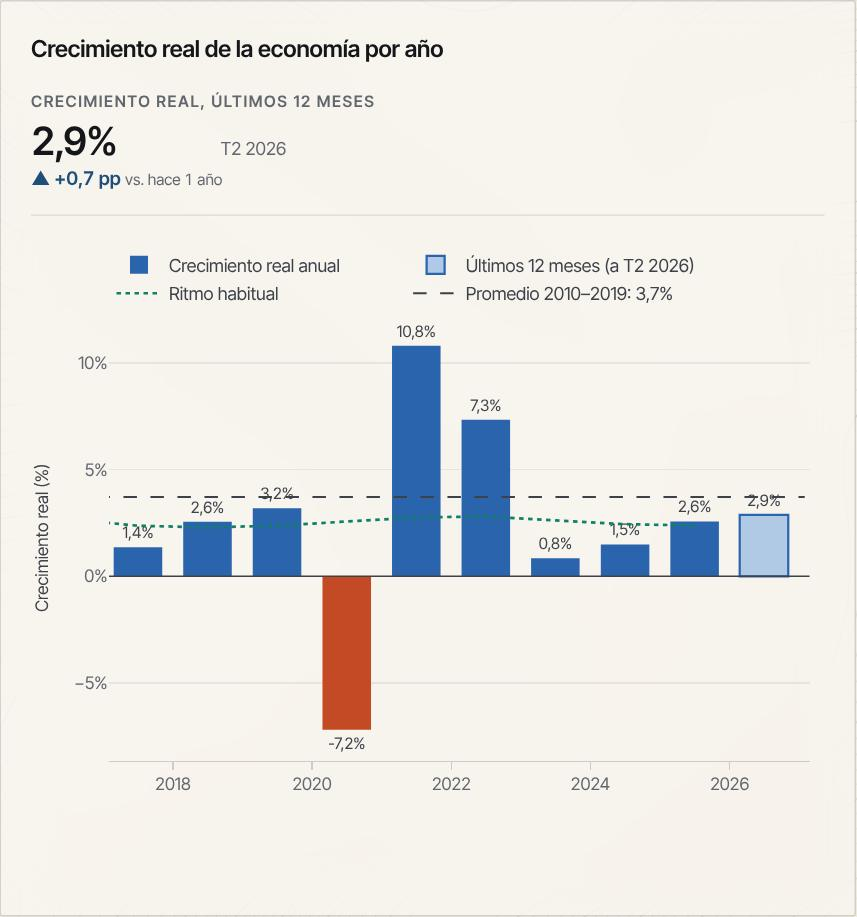
\includegraphics[width=\linewidth,height=0.42\textheight,keepaspectratio]{fig/g-pib-anual.jpg}\end{center}
\paragraph{Qué nos cuenta}
Resume el crecimiento real de la economía año por año: cuánto más (o menos) produjo el país frente al año anterior, descontando el efecto de los precios. Al agregar los cuatro trimestres se eliminan la estacionalidad y buena parte del ruido trimestral, lo que deja ver los grandes episodios: el auge de comienzos de la década de 2010, la desaceleración tras la caída del petróleo, la contracción de 2020 y el rebote posterior. El año todavía incompleto se muestra con los últimos 12 meses disponibles.

\begin{leer}[Cómo se lee]
Eje vertical: crecimiento real en \%. Cada barra es un año calendario completo; azul si la producción creció y naranja si cayó, con el valor escrito encima. La barra clara con borde azul aparece cuando el año en curso no ha terminado: es el crecimiento de los últimos 12 meses frente a los 12 previos, hasta el último trimestre publicado. La línea verde punteada es el ritmo habitual (promedio anual del crecimiento de la tendencia HP) y la línea gris discontinua, el promedio simple de 2010–2019. La vista inicial cubre unos diez años.
\end{leer}

\paragraph{Por qué importa}
La cifra anual es la que se usa para comparar a Colombia con otros países, para los presupuestos públicos y para las metas fiscales, porque no depende de la estacionalidad ni de un trimestre atípico. Ponerla frente al ritmo habitual y al promedio de la década previa a la pandemia permite juzgar si un año fue excepcional o si la economía se mueve dentro de su rango histórico.

\paragraph{Cómo interpretarlo}
\begin{itemize}
\item Una barra por encima de la línea verde indica un año de crecimiento superior a la tendencia; por debajo, inferior. La línea gris es una referencia fija para comparar con la década anterior a la pandemia.
\item La barra clara no es el dato del año: mezcla trimestres del año anterior y del actual, y cambia con cada publicación trimestral hasta que se completa el cuarto trimestre.
\item Tras años de contracción, el siguiente suele mostrar crecimiento alto por efecto base: la comparación parte de un nivel deprimido, como ocurrió en 2021.
\item El ritmo habitual se reestima cuando llegan datos nuevos y el DANE revisa los trimestres previos, de modo que barras y línea pueden moverse levemente entre publicaciones.
\end{itemize}
\begin{formulas}[Fórmulas]
\formula{Crecimiento real anual}{g\textsubscript{A} = ($\Sigma$\textsubscript{q$\in$A} Y\textsubscript{q} $\div$ $\Sigma$\textsubscript{q$\in$A−1} Y\textsubscript{q} − 1) $\times$ 100}{Y\textsubscript{q} = PIB real del trimestre q (datos originales); A = año calendario}
\formula{Últimos 12 meses}{g\textsubscript{12m} = ($\Sigma$\textsubscript{k=0..3} Y\textsubscript{t−k} $\div$ $\Sigma$\textsubscript{k=4..7} Y\textsubscript{t−k} − 1) $\times$ 100}{t = último trimestre publicado}
\formula{Ritmo habitual anual}{ḡ*\textsubscript{A} = (1 $\div$ 4) $\times$ $\Sigma$\textsubscript{q$\in$A} g*\textsubscript{q}}{g*\textsubscript{q} = crecimiento anual de la tendencia HP en el trimestre q}
\formula{Referencia 2010–2019}{ḡ = (1 $\div$ 10) $\times$ $\Sigma$\textsubscript{A=2010..2019} g\textsubscript{A}}{promedio simple de las tasas anuales}
\end{formulas}
\begin{metodo}[Metodología]
Crecimiento real anual = 100 $\times$ (PIB real del año / PIB real del año anterior − 1), sumando los cuatro trimestres de cada año (volúmenes encadenados, sin efecto de la inflación). Barra clara: últimos 12 meses frente a los 12 meses previos. Ritmo habitual: promedio anual del crecimiento de la tendencia (HP). Referencia: promedio simple 2010–2019.
\par\smallskip{\small\textbf{Fuente:} DANE, PIB trimestral a precios constantes (datos originales, base 2015)}
\end{metodo}

\section{¿A qué velocidad crece la economía?}

\subsection{Tres velocidades del crecimiento del PIB}
\label{g:g-velocidades}
\begin{center}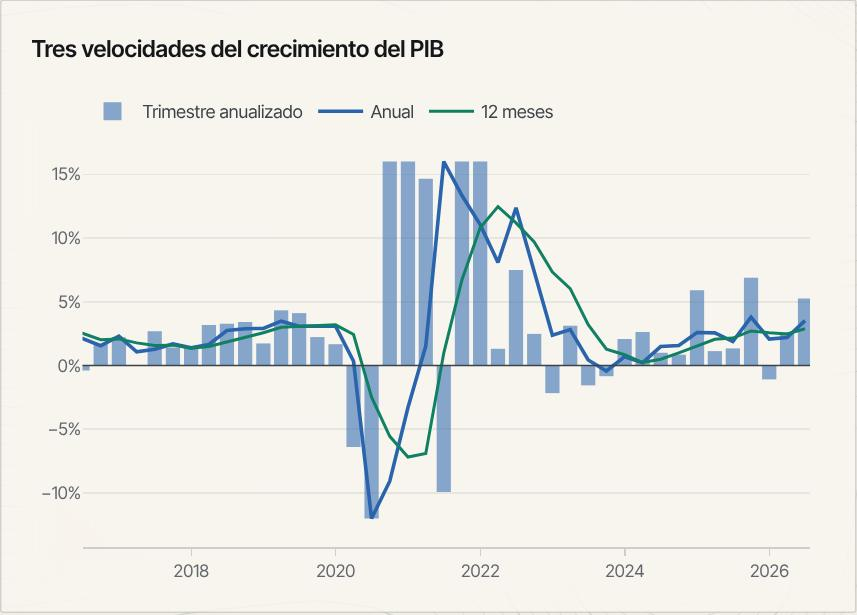
\includegraphics[width=\linewidth,height=0.42\textheight,keepaspectratio]{fig/g-velocidades.jpg}\end{center}
\paragraph{Qué nos cuenta}
Presenta tres maneras de medir el mismo crecimiento del PIB real, cada una con un horizonte distinto. La variación anual compara con el mismo trimestre del año anterior; la de 12 meses compara el último año completo con el anterior y es la más suave; el trimestre anualizado mide el impulso más reciente, como si el ritmo del último trimestre se mantuviera un año entero. Leídas juntas indican si la economía está acelerando o frenando antes de que lo refleje la cifra anual.

\begin{leer}[Cómo se lee]
Eje en \%, desde 2012. Línea azul: variación anual del PIB real (datos originales). Línea verde: suma de los últimos cuatro trimestres frente a los cuatro anteriores. Barras azul claro: variación del PIB desestacionalizado frente al trimestre anterior, elevada a ritmo anual. La línea horizontal en cero separa crecimiento de contracción. Para que la escala siga siendo legible, todos los valores se recortan entre −12\% y 16\%, lo que afecta sobre todo a 2020 y 2021.
\end{leer}

\paragraph{Por qué importa}
Las tasas anuales reaccionan con retraso: pueden seguir altas cuando la economía ya se frenó, o bajas cuando ya se está recuperando. El trimestre anualizado, convención de la Oficina de Análisis Económico de EE. UU. (BEA), es el que primero muestra los puntos de giro, y la medida de 12 meses es la que se compara con las cifras anuales oficiales. Comparar las tres evita conclusiones apresuradas a partir de un solo dato.

\paragraph{Cómo interpretarlo}
\begin{itemize}
\item Barras por encima de la línea azul: el ritmo reciente supera al anual, la economía está acelerando; por debajo, está frenando.
\item La línea verde cambia despacio: si gira, el cambio de tendencia ya acumula varios trimestres.
\item El trimestre anualizado multiplica por cuatro aproximadamente el ruido trimestral y depende del ajuste estacional, que se reestima con cada publicación; un solo trimestre alto o bajo no define una tendencia.
\item Los valores fuera del rango −12\% a 16\% aparecen topados en el borde: en 2020–2021 los datos reales fueron más extremos que lo que muestra el dibujo.
\end{itemize}
\begin{formulas}[Fórmulas]
\formula{Variación anual}{g\textsubscript{t} = (Y\textsubscript{t} $\div$ Y\textsubscript{t−4} − 1) $\times$ 100}{Y = PIB real, datos originales}
\formula{12 meses}{g\textsubscript{12m,t} = ($\Sigma$\textsubscript{k=0..3} Y\textsubscript{t−k} $\div$ $\Sigma$\textsubscript{k=4..7} Y\textsubscript{t−k} − 1) $\times$ 100}{sumas móviles de cuatro trimestres}
\formula{Trimestre anualizado}{a\textsubscript{t} = ((S\textsubscript{t} $\div$ S\textsubscript{t−1})\textsuperscript{4} − 1) $\times$ 100}{S = PIB real desestacionalizado}
\formula{Recorte gráfico}{valor dibujado = min(16; max(−12; x))}{x = cualquiera de las tres medidas}
\end{formulas}
\begin{metodo}[Metodología]
Anual: PIB real original frente al mismo trimestre del año anterior. 12 meses: suma de los últimos 4 trimestres frente a los 4 anteriores. Trimestre anualizado: ((PIB desestacionalizado t / t−1)\textasciicircum{}4 − 1) $\times$ 100, la convención de la Oficina de Análisis Económico de EE. UU. (BEA).
\par\smallskip{\small\textbf{Fuente:} DANE, PIB trimestral (anexos de producción a precios constantes y corrientes)}
\end{metodo}

\subsection{Crecimiento promedio por periodo}
\label{g:g-periodos}
\begin{center}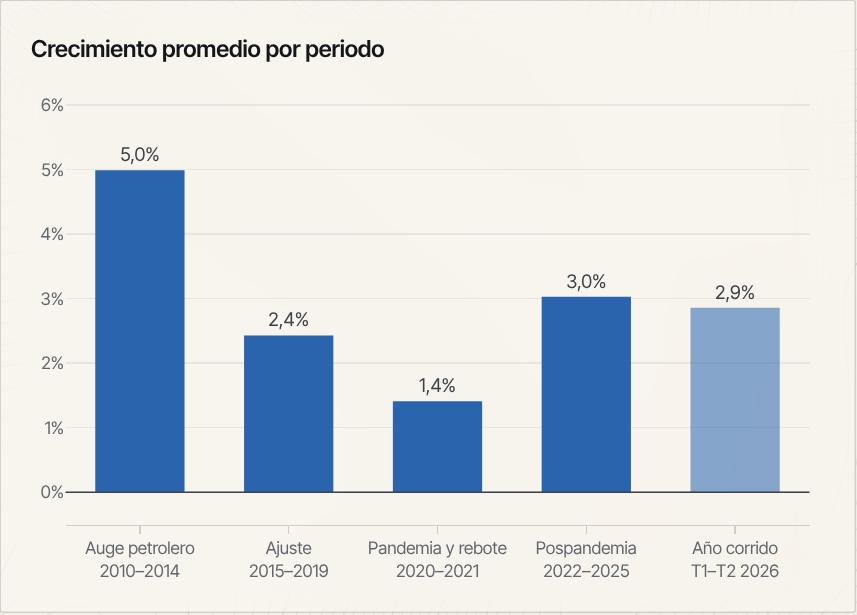
\includegraphics[width=\linewidth,height=0.42\textheight,keepaspectratio]{fig/g-periodos.jpg}\end{center}
\paragraph{Qué nos cuenta}
Condensa la historia reciente del crecimiento en etapas: el auge petrolero (2010–2014), el ajuste tras la caída del precio del crudo (2015–2019), la pandemia y el rebote (2020–2021) y la pospandemia, a partir de 2022, que se incluye solo cuando sus años están completos. Para cada etapa calcula el crecimiento anual compuesto del PIB real, es decir, la tasa constante que habría llevado la economía del nivel inicial al final. La última barra muestra el año corrido frente al mismo periodo del año anterior.

\begin{leer}[Cómo se lee]
Eje vertical en \%, con el valor escrito sobre cada barra. Las barras azul oscuro son los periodos completos; la barra azul claro es el año corrido (del primer trimestre al último publicado) y no es comparable en duración con las demás. La línea en cero separa crecimiento de contracción. El eje horizontal no es temporal: cada categoría es un periodo con sus años indicados en la etiqueta.
\end{leer}

\paragraph{Por qué importa}
Promediar por etapas permite separar la tendencia de largo plazo de los vaivenes de cada trimestre y comparar regímenes económicos distintos: un periodo con petróleo caro, uno de ajuste y uno de choque sanitario. Para un inversionista, el crecimiento compuesto de cada etapa es la referencia de cuánto puede expandirse el mercado interno en condiciones similares.

\paragraph{Cómo interpretarlo}
\begin{itemize}
\item La tasa compuesta es menor que el promedio simple de las tasas anuales cuando estas son volátiles: por eso el periodo de pandemia muestra un crecimiento moderado aunque incluye una caída fuerte y un rebote fuerte.
\item La barra del año corrido puede cambiar bastante con cada trimestre nuevo y con las revisiones del DANE; compárela con precaución frente a periodos de cinco años.
\item Los cortes de los periodos son una convención basada en hitos conocidos; otros cortes darían promedios distintos.
\end{itemize}
\begin{formulas}[Fórmulas]
\formula{Tasa anual compuesta}{c = ((Y\textsubscript{A1} $\div$ Y\textsubscript{A0−1})\textsuperscript{1 $\div$ n} − 1) $\times$ 100}{Y\textsubscript{A} = PIB real del año A (suma de 4 trimestres); A0 y A1 = primer y último año del periodo; n = A1 − A0 + 1}
\formula{Año corrido}{c\textsubscript{yc} = ($\Sigma$\textsubscript{q$\le$t, año actual} Y\textsubscript{q} $\div$ $\Sigma$\textsubscript{mismos trimestres, año anterior} Y\textsubscript{q} − 1) $\times$ 100}{t = último trimestre publicado}
\end{formulas}
\begin{metodo}[Metodología]
Tasa compuesta anual: (PIB del último año / PIB del año previo al periodo)\textasciicircum{}(1/años) − 1, con PIB real anual (suma de trimestres). Los periodos siguen hitos conocidos: auge del petróleo (2010–2014), caída del precio y ajuste (2015–2019), pandemia (2020–2021).
\par\smallskip{\small\textbf{Fuente:} DANE, PIB trimestral (anexos de producción a precios constantes y corrientes)}
\end{metodo}

\section{¿Cuánto es crecimiento real y cuánto son precios?}

\subsection{PIB en pesos corrientes y PIB real}
\label{g:g-real-nominal}
\begin{center}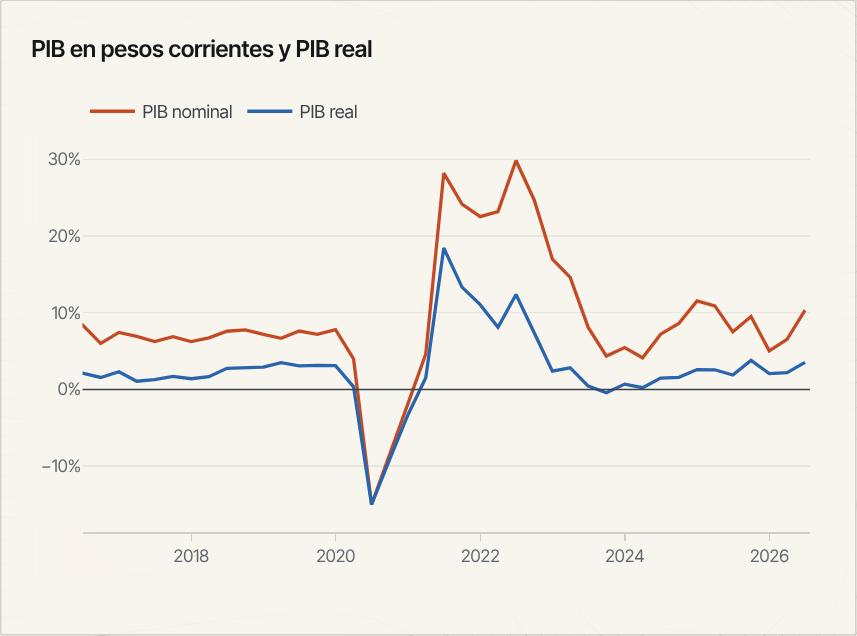
\includegraphics[width=\linewidth,height=0.42\textheight,keepaspectratio]{fig/g-real-nominal.jpg}\end{center}
\paragraph{Qué nos cuenta}
Compara el crecimiento del PIB medido en pesos de cada momento (nominal) con el crecimiento del PIB a precios constantes de 2015 (real). El nominal refleja a la vez cuánto más se produce y cuánto más caro se vende; el real aísla las cantidades. La distancia entre las dos líneas es, por tanto, el aumento de los precios de todo lo que produce la economía, conocido como deflactor implícito del PIB.

\begin{leer}[Cómo se lee]
Eje en \%, variación anual desde 2012. Línea naranja: PIB nominal (billones de pesos corrientes) frente al mismo trimestre del año anterior. Línea azul: PIB real (volúmenes encadenados, base 2015) con la misma comparación. Ambas en datos originales. La línea en cero marca el paso de crecimiento a caída. Los valores se recortan entre −15\% y 30\% para conservar la escala.
\end{leer}

\paragraph{Por qué importa}
Los ingresos de las empresas, los salarios, el recaudo de impuestos y la relación deuda/PIB se mueven con el PIB nominal, no con el real. Una economía puede mostrar un crecimiento nominal alto sin que aumente la producción, solo porque suben los precios. Separar ambos componentes evita confundir inflación con dinamismo y explica por qué ciertos indicadores fiscales mejoran o empeoran aunque la actividad real no cambie.

\paragraph{Cómo interpretarlo}
\begin{itemize}
\item Una distancia amplia entre las líneas indica inflación alta de toda la economía; si se estrecha, los precios crecen menos. La diferencia se analiza en el gráfico del deflactor frente al IPC.
\item Si la línea naranja cae más que la azul, bajan los precios de lo producido, algo que ocurre cuando caen los precios del petróleo, el carbón u otras exportaciones.
\item El PIB nominal no se publica desestacionalizado en esta comparación: ambas series usan datos originales para que la diferencia sea coherente.
\end{itemize}
\begin{formulas}[Fórmulas]
\formula{Crecimiento nominal}{n\textsubscript{t} = (N\textsubscript{t} $\div$ N\textsubscript{t−4} − 1) $\times$ 100}{N = PIB a precios corrientes (billones de pesos)}
\formula{Crecimiento real}{g\textsubscript{t} = (Y\textsubscript{t} $\div$ Y\textsubscript{t−4} − 1) $\times$ 100}{Y = PIB a precios constantes de 2015}
\formula{Relación entre ambos}{(1 + n) = (1 + g) $\times$ (1 + $\pi$\textsubscript{D})  $\Rightarrow$  n $\approx$ g + $\pi$\textsubscript{D}}{$\pi$\textsubscript{D} = variación anual del deflactor del PIB (en tasas, no en \%)}
\end{formulas}
\begin{metodo}[Metodología]
Variación anual del PIB a precios corrientes (billones de pesos) y a precios constantes de 2015 (series originales).
\par\smallskip{\small\textbf{Fuente:} DANE, PIB trimestral (anexos de producción a precios constantes y corrientes)}
\end{metodo}

\subsection{Precios de lo que se produce frente a precios de lo que se consume}
\label{g:g-deflactor}
\begin{center}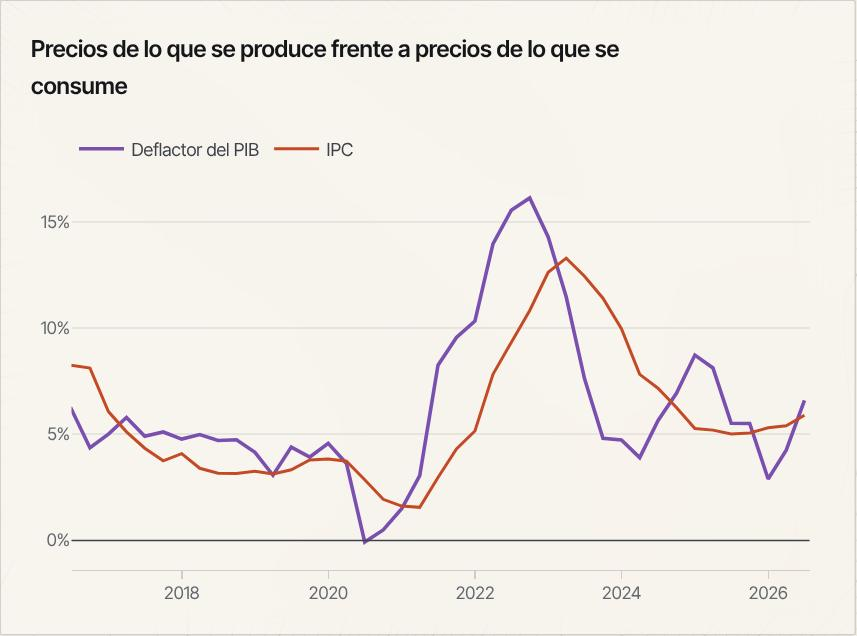
\includegraphics[width=\linewidth,height=0.42\textheight,keepaspectratio]{fig/g-deflactor.jpg}\end{center}
\paragraph{Qué nos cuenta}
Compara dos medidas de inflación que miran canastas distintas. El deflactor implícito del PIB recoge los precios de todo lo que se produce en Colombia, incluidas las exportaciones (petróleo, carbón, café) y excluidas las importaciones. El Índice de Precios al Consumidor (IPC) recoge los precios de lo que compran los hogares, incluidos bienes importados. Cuando divergen, la razón principal suele ser el cambio en los términos de intercambio: la relación entre los precios de lo que el país vende y lo que compra al exterior.

\begin{leer}[Cómo se lee]
Eje en \%, desde 2012. Línea morada: variación anual del deflactor implícito del PIB, calculado como PIB nominal sobre PIB real de cada trimestre. Línea naranja: inflación anual del IPC, promediando los tres meses de cada trimestre. La línea en cero marca deflación. Ambas se refieren al mismo trimestre, de modo que la distancia vertical entre ellas se lee directamente en puntos porcentuales.
\end{leer}

\paragraph{Por qué importa}
El IPC es el objetivo de política monetaria del Banco de la República; el deflactor determina el valor en pesos de la producción y, por tanto, de los ingresos de empresas y del Gobierno. Cuando el deflactor supera al IPC, el país gana poder de compra frente al exterior (mejores términos de intercambio) y suelen mejorar el recaudo y las cuentas externas; cuando va por debajo, ocurre lo contrario aunque la inflación al consumidor no cambie.

\paragraph{Cómo interpretarlo}
\begin{itemize}
\item Morada por encima de la naranja: suben más los precios de lo que Colombia produce y exporta que los de la canasta de los hogares, típico de periodos de petróleo caro.
\item Morada por debajo: los precios de los productos exportados caen o suben menos; el ingreso nacional crece menos que lo que sugiere el PIB real.
\item El deflactor es una medida implícita: se revisa cada vez que el DANE revisa el PIB nominal o real, y en trimestres de choque puede moverse de forma brusca.
\item La relación con los términos de intercambio se puede contrastar en la página del sector externo.
\end{itemize}
\begin{formulas}[Fórmulas]
\formula{Deflactor implícito}{D\textsubscript{t} = N\textsubscript{t} $\div$ Y\textsubscript{t}}{N = PIB nominal; Y = PIB real (base 2015), datos originales}
\formula{Inflación del deflactor}{$\pi$\textsubscript{D,t} = (D\textsubscript{t} $\div$ D\textsubscript{t−4} − 1) $\times$ 100}{variación anual del trimestre t}
\formula{IPC trimestral}{$\pi$\textsubscript{IPC,t} = (1 $\div$ 3) $\times$ $\Sigma$\textsubscript{m$\in$t} $\pi$\textsubscript{m}}{$\pi$\textsubscript{m} = inflación anual del IPC en el mes m}
\end{formulas}
\begin{metodo}[Metodología]
Deflactor implícito = PIB nominal / PIB real; se muestra su variación anual. El IPC es el promedio trimestral de la inflación anual. La diferencia refleja sobre todo los términos de intercambio: el deflactor incluye exportaciones y excluye importaciones (Kohli, 2004).
\par\smallskip{\small\textbf{Fuente:} DANE (PIB nominal y real) y DANE-IPC; cálculo propio}
\end{metodo}

\section{¿Quién explica el crecimiento?}

\subsection{Aportes al crecimiento por grandes grupos}
\label{g:g-aportes-grupos}
\begin{center}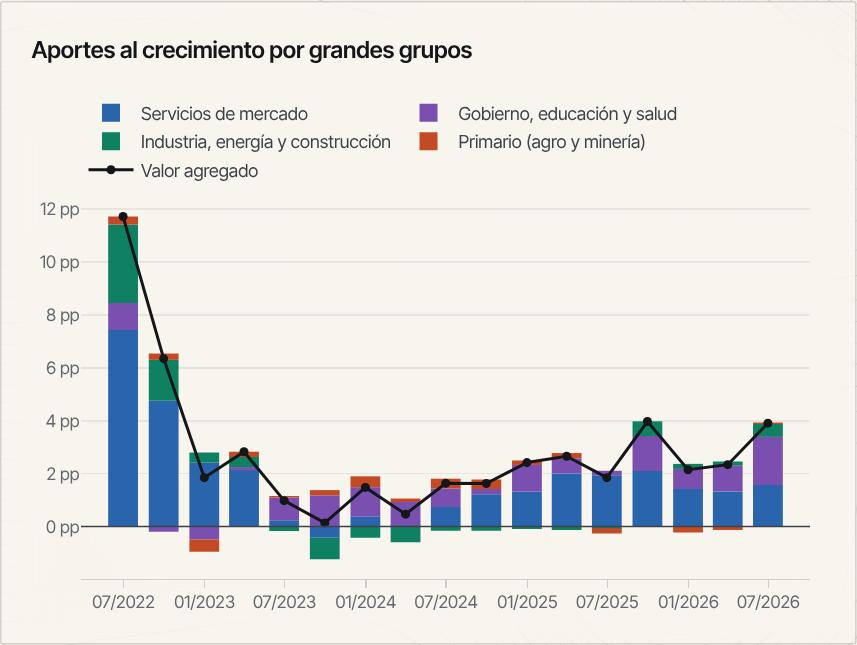
\includegraphics[width=\linewidth,height=0.42\textheight,keepaspectratio]{fig/g-aportes-grupos.jpg}\end{center}
\paragraph{Qué nos cuenta}
Descompone el crecimiento anual del valor agregado en cuatro grandes grupos de actividades: sector primario (agro y minería), industria, energía y construcción, servicios de mercado, y Gobierno, educación y salud. Cada bloque indica cuántos puntos del crecimiento total explica ese grupo, combinando su tamaño y su ritmo de crecimiento. Así se ve quién está empujando la economía y quién la está frenando en cada trimestre.

\begin{leer}[Cómo se lee]
Eje en puntos porcentuales (pp), últimos cuatro años, un grupo de barras por trimestre. Barras apiladas: azul, servicios de mercado (comercio, transporte, turismo, comunicaciones, finanzas, inmobiliarias, servicios profesionales y entretenimiento); morado, Gobierno, educación y salud; verde, industria, electricidad, gas, agua y construcción; naranja, primario. Los aportes negativos se apilan por debajo de cero. La línea negra con puntos es la suma de todos los aportes, que aproxima el crecimiento anual del valor agregado.
\end{leer}

\paragraph{Por qué importa}
Un mismo crecimiento puede tener orígenes muy distintos: no es igual que lo impulsen los servicios privados que el gasto público o la minería. La composición informa sobre la sostenibilidad del ciclo, la generación de empleo y los sectores donde se concentran ingresos y utilidades, información útil para evaluar exposición sectorial en carteras y créditos.

\paragraph{Cómo interpretarlo}
\begin{itemize}
\item Un grupo pequeño que crece mucho puede aportar menos que un grupo grande que crece poco: el aporte pondera el crecimiento por el peso en la economía.
\item Si la mayor parte de la barra viene del bloque morado, el crecimiento depende del sector público y servicios sociales; el gráfico de la economía con y sin Gobierno lo cuantifica.
\item La línea mide el valor agregado, no el PIB: falta el aporte de los impuestos netos de subvenciones y, como los volúmenes encadenados no son aditivos, la suma puede diferir unas décimas del crecimiento publicado.
\item El grupo de Gobierno incluye la educación y la salud privadas: es una aproximación al sector público, no una medida exacta.
\end{itemize}
\begin{formulas}[Fórmulas]
\formula{Aporte de un sector}{a\textsubscript{i,t} = (X\textsubscript{i,t} − X\textsubscript{i,t−4}) $\div$ VA\textsubscript{t−4} $\times$ 100 = g\textsubscript{i,t} $\times$ w\textsubscript{i,t−4}}{X\textsubscript{i} = valor agregado real del sector i; VA = valor agregado total; g = variación anual; w = participación en el VA}
\formula{Aporte de un grupo}{A\textsubscript{G,t} = $\Sigma$\textsubscript{i$\in$G} a\textsubscript{i,t}}{G = conjunto de sectores CIIU del grupo}
\formula{Total (línea)}{T\textsubscript{t} = $\Sigma$\textsubscript{i=1..12} a\textsubscript{i,t}}{suma de los aportes de las 12 agrupaciones CIIU}
\end{formulas}
\begin{metodo}[Metodología]
Aporte del sector = variación anual $\times$ participación en el valor agregado del año anterior (precios constantes); los 12 sectores se agrupan en 4. Los aportes suman el valor agregado, no el PIB: falta el aporte de los impuestos netos de subvenciones, y el encadenamiento genera pequeñas diferencias.
\par\smallskip{\small\textbf{Fuente:} DANE, PIB por actividad económica; cálculo propio}
\end{metodo}

\subsection{La economía con y sin Gobierno}
\label{g:g-sin-gobierno}
\begin{center}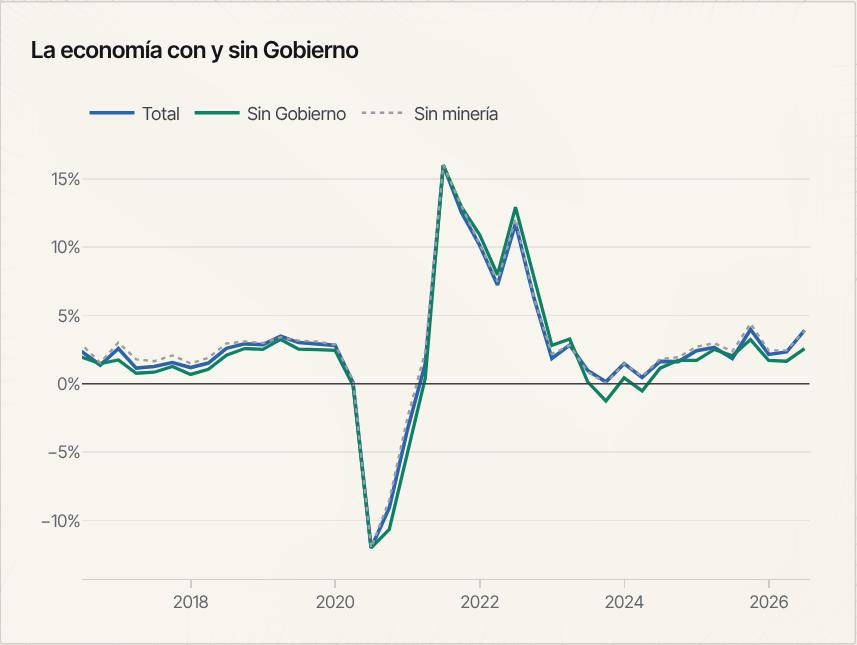
\includegraphics[width=\linewidth,height=0.42\textheight,keepaspectratio]{fig/g-sin-gobierno.jpg}\end{center}
\paragraph{Qué nos cuenta}
Muestra cuánto crecería el valor agregado si se excluyera un sector concreto: el de Gobierno, educación y salud (secciones O, P y Q de la Clasificación Industrial Internacional Uniforme, CIIU) o la minería. Sirve para saber si el crecimiento total está sostenido por la actividad privada y diversificada o descansa en el sector público o en los hidrocarburos y el carbón.

\begin{leer}[Cómo se lee]
Eje en \%, variación anual desde 2012. Línea azul: crecimiento total del valor agregado (suma de los aportes de los 12 sectores). Línea verde: crecimiento del resto de la economía sin Gobierno, educación y salud. Línea gris punteada: crecimiento sin minería. La línea en cero separa crecimiento de contracción. Los valores se recortan entre −12\% y 16\% para que 2020–2021 no aplasten la escala.
\end{leer}

\paragraph{Por qué importa}
El sector público crece por decisiones presupuestarias, no por la demanda del mercado, y la minería depende de precios internacionales y de la geología. Si el resto de la economía crece mucho menos que el total, el dinamismo es más estrecho y menos ligado al consumo y la inversión privados, lo que importa para leer el empleo formal, el crédito y las ventas de las empresas.

\paragraph{Cómo interpretarlo}
\begin{itemize}
\item Verde por debajo de azul: el sector Gobierno, educación y salud crece más que el resto y sostiene el total; verde por encima: el sector privado y los demás servicios van más rápido.
\item Gris por encima de azul: la minería está restando al crecimiento; por debajo, lo está sumando.
\item El sector O-P-Q incluye la educación y la salud privadas, por lo que «sin Gobierno» es una aproximación al crecimiento privado.
\item El cálculo usa aportes aproximados de volúmenes encadenados, que no son exactamente aditivos; diferencias de pocas décimas no son significativas.
\end{itemize}
\begin{formulas}[Fórmulas]
\formula{Crecimiento sin el sector X}{g\textsubscript{−X,t} = 100 $\times$ ($\Sigma$\textsubscript{i} a\textsubscript{i,t} − a\textsubscript{X,t}) $\div$ ($\Sigma$\textsubscript{i} w\textsubscript{i,t} − w\textsubscript{X,t})}{a = aporte en pp; w = participación en el valor agregado en \%; $\Sigma$ sobre los 12 sectores}
\formula{Total (línea azul)}{T\textsubscript{t} = $\Sigma$\textsubscript{i} a\textsubscript{i,t}}{a\textsubscript{i,t} = (X\textsubscript{i,t} − X\textsubscript{i,t−4}) $\div$ VA\textsubscript{t−4} $\times$ 100}
\end{formulas}
\begin{metodo}[Metodología]
Crecimiento sin el sector X = (suma de aportes − aporte de X) / (suma de participaciones − participación de X). El sector «Gobierno, educación y salud» (secciones O, P y Q del CIIU) incluye también educación y salud privadas: es una aproximación al sector público.
\par\smallskip{\small\textbf{Fuente:} DANE, PIB por actividad económica; cálculo propio}
\end{metodo}

\section{¿Qué sectores impulsan la economía?}

\subsection{Crecimiento anual por sector (T2 2026)}
\label{g:g-sec-barras}
\begin{center}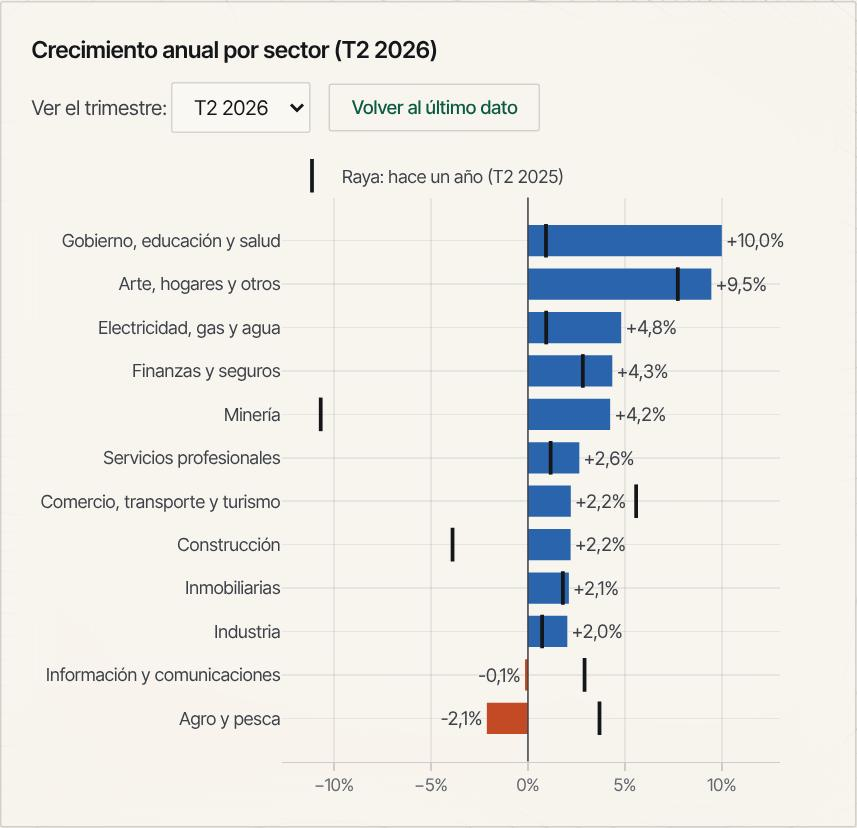
\includegraphics[width=\linewidth,height=0.42\textheight,keepaspectratio]{fig/g-sec-barras.jpg}\end{center}
\paragraph{Qué nos cuenta}
Ordena las 12 grandes ramas de actividad de las cuentas nacionales (agrupaciones de la CIIU Rev. 4) según cuánto creció cada una frente al mismo trimestre del año anterior. Junto a cada barra aparece el dato de un año antes, de modo que se ve no solo quién crece más, sino quién se está acelerando y quién se está frenando. Es la fotografía sectorial del trimestre más reciente, o de cualquier trimestre elegido en el selector.

\begin{leer}[Cómo se lee]
Eje horizontal en \% de variación anual real; los sectores están ordenados de mayor (arriba) a menor crecimiento. Barra azul: el sector creció; barra naranja: cayó; el valor está escrito al final de cada barra. La raya negra vertical sobre cada fila es la variación anual del mismo sector un año antes. La línea en cero separa crecimiento de caída. Al pasar el cursor se ve el peso del sector en el valor agregado y su aporte en pp. El selector permite ver otro trimestre y el botón vuelve al último; también se puede elegir haciendo clic en el mapa de calor.
\end{leer}

\paragraph{Por qué importa}
El agregado esconde dispersión: un PIB moderado puede convivir con sectores en auge y otros en recesión. Para un inversionista, conocer qué sectores se aceleran o se contraen orienta el análisis de empresas, crédito y empleo, y permite distinguir si un cambio en el PIB proviene de un sector grande o de muchos sectores a la vez.

\paragraph{Cómo interpretarlo}
\begin{itemize}
\item Barra más larga que la raya: el sector crece más que hace un año (aceleración); más corta: se frena. Si la barra es naranja y la raya está a la derecha del cero, el sector pasó de crecer a caer.
\item El crecimiento alto de un sector pequeño pesa poco en el total; el aporte (en el recuadro flotante) combina crecimiento y tamaño.
\item Los sectores con alta volatilidad, como minería, agro o construcción, pueden mostrar cambios grandes sin que cambie la tendencia de fondo.
\item Los datos son originales, sin desestacionalizar, y se revisan en cada publicación del DANE; los aportes son aproximados porque los volúmenes encadenados no suman exactamente.
\end{itemize}
\begin{formulas}[Fórmulas]
\formula{Variación anual del sector}{g\textsubscript{i,t} = (X\textsubscript{i,t} $\div$ X\textsubscript{i,t−4} − 1) $\times$ 100}{X\textsubscript{i,t} = valor agregado real del sector i (volúmenes encadenados, base 2015)}
\formula{Peso en la economía}{w\textsubscript{i,t} = X\textsubscript{i,t} $\div$ VA\textsubscript{t} $\times$ 100}{VA = valor agregado total del mismo trimestre}
\formula{Aporte al crecimiento}{a\textsubscript{i,t} = (X\textsubscript{i,t} − X\textsubscript{i,t−4}) $\div$ VA\textsubscript{t−4} $\times$ 100}{en pp del valor agregado de hace un año}
\end{formulas}
\begin{metodo}[Metodología]
12 agrupaciones CIIU Rev. 4 (volúmenes encadenados, año base 2015, datos originales). Crecimiento anual frente al mismo trimestre del año anterior; la raya vertical es el dato de un año antes. Aporte = cambio del nivel del sector en un año / valor agregado total de hace un año.
\par\smallskip{\small\textbf{Fuente:} DANE, PIB trimestral (anexos de producción a precios constantes y corrientes)}
\end{metodo}

\subsection{Mapa del crecimiento por sector, trimestre a trimestre}
\label{g:g-sec-mapa}
\begin{center}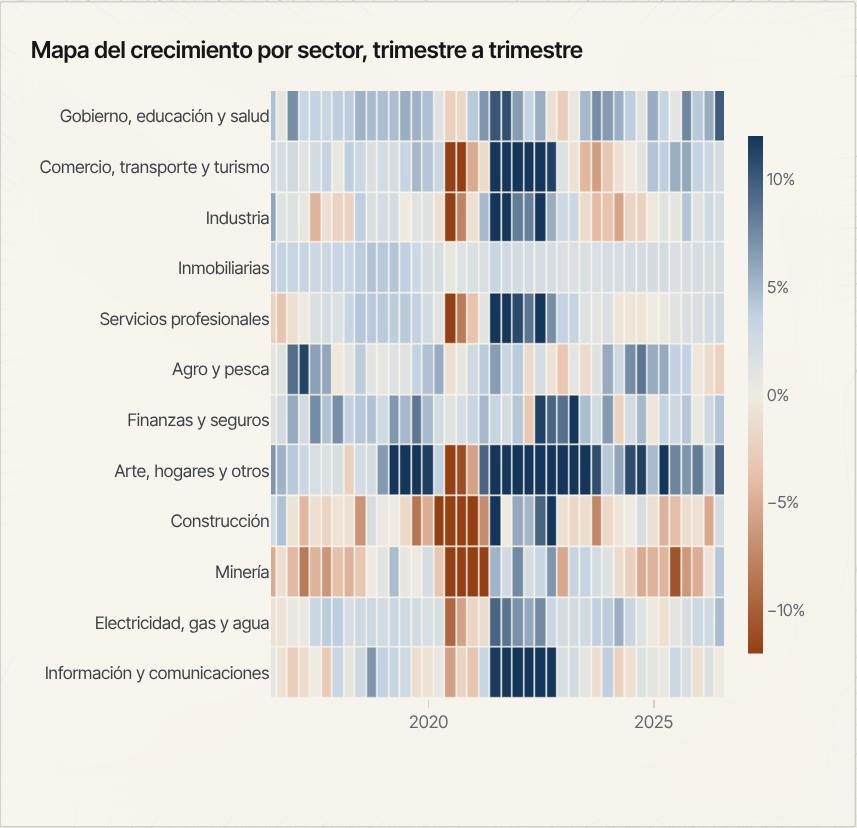
\includegraphics[width=\linewidth,height=0.42\textheight,keepaspectratio]{fig/g-sec-mapa.jpg}\end{center}
\paragraph{Qué nos cuenta}
Reúne en una sola imagen el crecimiento anual de los 12 sectores en cada trimestre. Permite seguir la historia sectorial completa: qué ramas se hundieron en 2020, cuáles se recuperaron primero, cuáles llevan varios trimestres en terreno negativo y si las caídas o los auges son generalizados o se concentran en pocas actividades.

\begin{leer}[Cómo se lee]
Cada fila es un sector, ordenado por su peso en el valor agregado del último trimestre (los más grandes arriba); cada columna es un trimestre. El color indica la variación anual real: blanco cerca de cero, azul cada vez más intenso para crecimientos altos y naranja para caídas. La escala de color se satura en $\pm$12\%: valores más extremos se ven con el color del borde, y el recuadro flotante muestra el valor exacto. La vista inicial cubre los últimos cinco años; al hacer clic en una casilla, el gráfico de barras pasa a ese trimestre.
\end{leer}

\paragraph{Por qué importa}
Un mapa de calor permite ver de un vistazo la persistencia y la amplitud de los movimientos sectoriales, algo difícil de captar con líneas superpuestas. Para un inversionista, señala sectores con debilidad o fortaleza sostenida, que es la información relevante para evaluar ciclos de ingresos y riesgo de crédito por actividad.

\paragraph{Cómo interpretarlo}
\begin{itemize}
\item Columnas casi todas naranjas indican una contracción generalizada (como en 2020); columnas mixtas, un ciclo con ganadores y perdedores.
\item Una fila con naranja persistente revela un sector en declive o en ajuste prolongado, aunque el agregado crezca.
\item El orden por tamaño ayuda a ponderar: un cambio de color en las filas superiores mueve el PIB mucho más que en las inferiores.
\item Los datos originales pueden mostrar saltos por efectos de calendario o base; el índice de difusión resume cuántas casillas son positivas en cada trimestre.
\end{itemize}
\begin{formulas}[Fórmulas]
\formula{Valor de cada casilla}{g\textsubscript{i,t} = (X\textsubscript{i,t} $\div$ X\textsubscript{i,t−4} − 1) $\times$ 100}{X\textsubscript{i,t} = valor agregado real del sector i en el trimestre t}
\formula{Color}{c = min(12; max(−12; g\textsubscript{i,t}))}{escala divergente centrada en cero}
\end{formulas}
\begin{metodo}[Metodología]
Crecimiento anual de cada sector por trimestre. La escala de color se recorta en $\pm$12\% para que 2020 no oculte el resto; el recuadro flotante muestra el valor exacto.
\par\smallskip{\small\textbf{Fuente:} DANE, PIB trimestral (anexos de producción a precios constantes y corrientes)}
\end{metodo}

\section{¿Cuántos sectores crecen y cómo van frente a su historia?}

\subsection{Sectores que crecen, de 12}
\label{g:g-sectores-crecen}
\begin{center}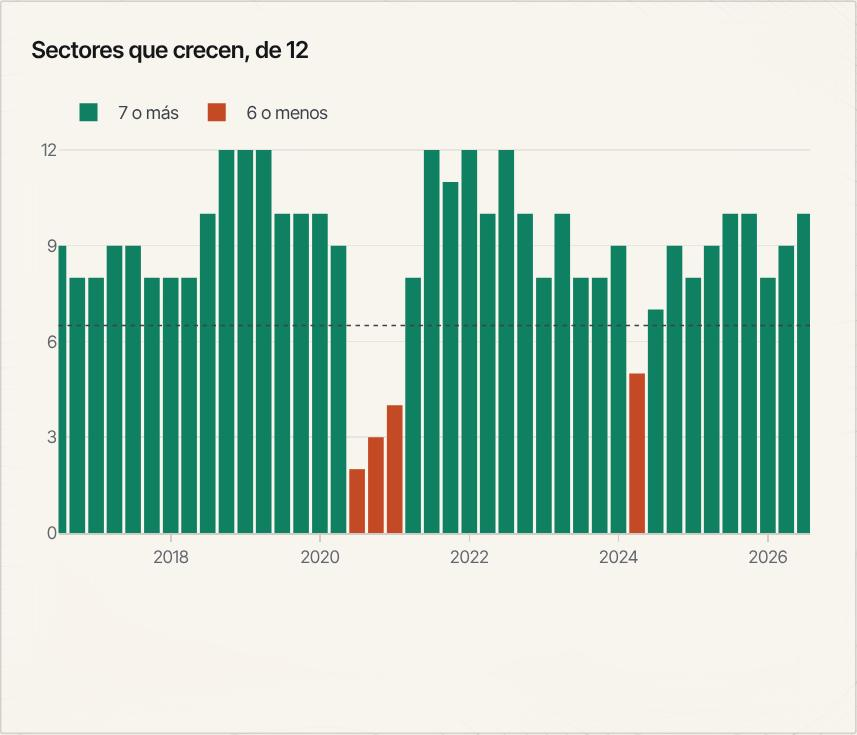
\includegraphics[width=\linewidth,height=0.42\textheight,keepaspectratio]{fig/g-sectores-crecen.jpg}\end{center}
\paragraph{Qué nos cuenta}
Cuenta, trimestre a trimestre, cuántos de los 12 sectores de la economía producen más que un año antes. Es un índice de difusión, en la tradición de Burns y Mitchell (1946): no mide cuánto crece la economía, sino qué tan extendido está el crecimiento. Un PIB que sube con pocos sectores es más frágil que uno que sube con casi todos.

\begin{leer}[Cómo se lee]
Eje vertical de 0 a 12 sectores, desde 2010. Cada barra es un trimestre. Barras verdes: 7 o más sectores crecen (crecimiento extendido); barras naranjas: 6 o menos. La línea punteada en 6,5 marca la mitad y separa ambos casos. Un sector cuenta como creciente si su variación anual real es mayor que cero, sin importar su tamaño.
\end{leer}

\paragraph{Por qué importa}
La amplitud complementa la magnitud: en las expansiones sólidas la mayoría de los sectores crece a la vez, mientras que en las fases de debilidad el crecimiento se concentra. Para un inversionista, una difusión alta reduce la dependencia de un solo motor y suele acompañar mejoras en empleo y crédito; una difusión baja indica que el dato agregado descansa en pocas actividades.

\paragraph{Cómo interpretarlo}
\begin{itemize}
\item Barras verdes persistentes acompañan expansiones amplias; una racha de barras naranjas, aunque el PIB crezca, señala un crecimiento estrecho.
\item El índice no pondera por tamaño: un trimestre con 10 sectores creciendo puede tener un PIB bajo si los sectores grandes caen. Compárelo con el gráfico de aportes.
\item Un sector con crecimiento de 0,1\% cuenta igual que uno con 10\%; cambios pequeños alrededor de cero pueden mover el conteo sin cambio económico relevante.
\end{itemize}
\begin{formulas}[Fórmulas]
\formula{Índice de difusión}{D\textsubscript{t} = $\Sigma$\textsubscript{i=1..12} 1[g\textsubscript{i,t} > 0]}{1[$\cdot$] = 1 si la condición se cumple y 0 si no; g\textsubscript{i,t} = variación anual real del sector i}
\end{formulas}
\begin{metodo}[Metodología]
Índice de difusión (Burns y Mitchell, 1946): número de los 12 sectores con variación anual positiva en cada trimestre.
\par\smallskip{\small\textbf{Fuente:} DANE, PIB por actividad económica; cálculo propio}
\end{metodo}

\subsection{Cada sector frente a su propia historia}
\label{g:g-sector-historia}
\begin{center}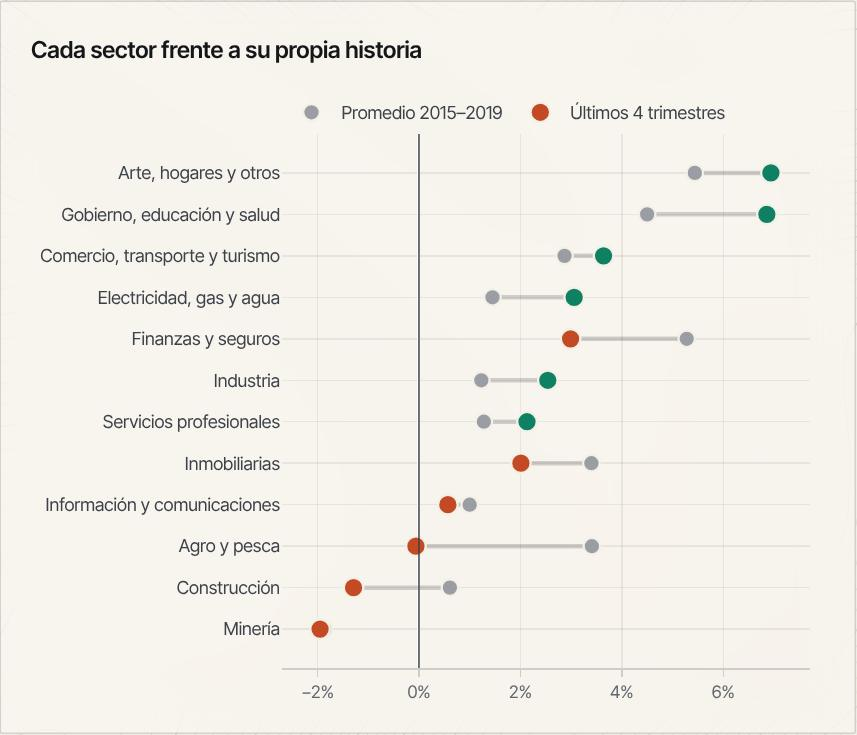
\includegraphics[width=\linewidth,height=0.42\textheight,keepaspectratio]{fig/g-sector-historia.jpg}\end{center}
\paragraph{Qué nos cuenta}
Compara el crecimiento reciente de cada sector con su propio desempeño en 2015–2019, un periodo previo a la pandemia sin choques extremos. Responde si cada actividad va hoy más rápido o más lento de lo que era normal para ella, algo que el ranking de crecimiento no muestra porque cada sector tiene su propio ritmo típico.

\begin{leer}[Cómo se lee]
Eje horizontal en \% de variación anual real. Cada fila es un sector, ordenado de menor (abajo) a mayor (arriba) crecimiento reciente. Punto gris: promedio de la variación anual de 2015T1 a 2019T4. Punto de color: promedio de los últimos cuatro trimestres publicados; verde si supera al promedio histórico y naranja si queda por debajo. La barra gris clara une los dos puntos y su longitud es la distancia entre hoy y la historia. La línea vertical marca el cero.
\end{leer}

\paragraph{Por qué importa}
Un crecimiento de 2\% puede ser bueno para un sector maduro y malo para uno que solía crecer al 6\%. Medir contra la propia historia identifica cambios estructurales o cíclicos por actividad, útiles para valorar empresas y para entender qué sectores explican que la economía crezca por encima o por debajo de su ritmo previo.

\paragraph{Cómo interpretarlo}
\begin{itemize}
\item Muchos puntos verdes indican que la mayoría de sectores supera su ritmo habitual; muchos naranjas, una economía que crece por debajo de su historia en forma extendida.
\item Una distancia grande hacia la izquierda en un sector importante (por ejemplo, minería o construcción) puede explicar buena parte de la diferencia entre el crecimiento actual y el previo a la pandemia.
\item El promedio de cuatro trimestres suaviza el ruido, pero incluye trimestres con datos originales y revisiones; el punto de color se mueve con cada publicación.
\item El periodo 2015–2019 incluye la caída del petróleo: no es un «ideal», solo una referencia reciente sin pandemia.
\end{itemize}
\begin{formulas}[Fórmulas]
\formula{Promedio histórico}{h\textsubscript{i} = (1 $\div$ 20) $\times$ $\Sigma$\textsubscript{t=2015T1..2019T4} g\textsubscript{i,t}}{g\textsubscript{i,t} = variación anual real del sector i en el trimestre t}
\formula{Promedio reciente}{u\textsubscript{i} = (1 $\div$ 4) $\times$ $\Sigma$\textsubscript{k=0..3} g\textsubscript{i,T−k}}{T = último trimestre publicado}
\formula{Color}{verde si u\textsubscript{i} $\ge$ h\textsubscript{i}; naranja en caso contrario}{u\textsubscript{i} = promedio reciente; h\textsubscript{i} = promedio 2015–2019 del sector i}
\end{formulas}
\begin{metodo}[Metodología]
Promedio simple de la variación anual de cada sector en 2015T1–2019T4 frente al promedio de los últimos 4 trimestres publicados.
\par\smallskip{\small\textbf{Fuente:} DANE, PIB por actividad económica; cálculo propio}
\end{metodo}

\section{¿Quién gasta? El PIB por el lado de la demanda}

\subsection{Aportes al crecimiento del PIB por componente de la demanda}
\label{g:g-demanda-aportes}
\begin{center}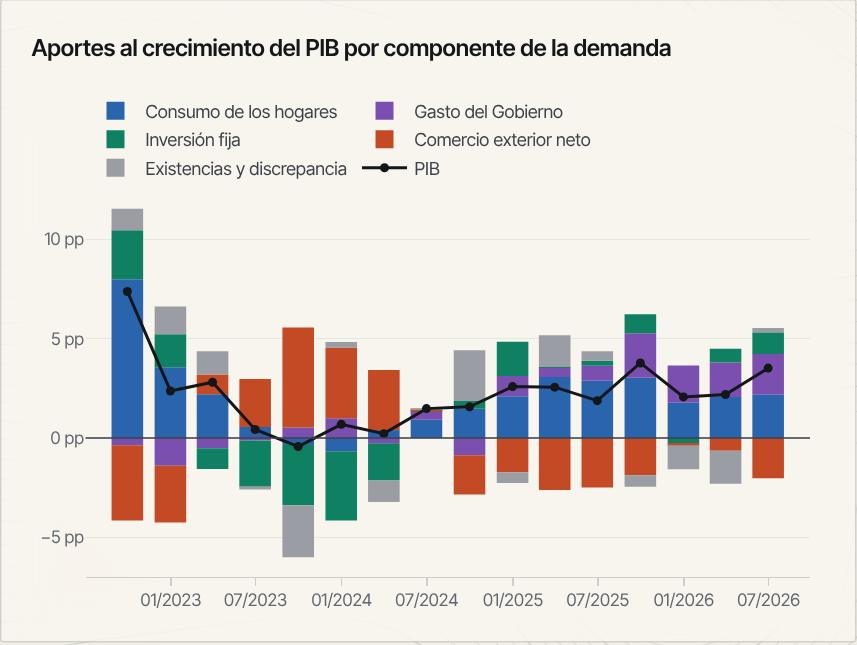
\includegraphics[width=\linewidth,height=0.42\textheight,keepaspectratio]{fig/g-demanda-aportes.jpg}\end{center}
\paragraph{Qué nos cuenta}
Mira el crecimiento desde el lado del gasto: cuántos puntos del crecimiento anual del PIB explican el consumo de los hogares, el gasto del Gobierno, la inversión fija y el comercio exterior neto. Es la otra cara de los aportes por sector: allí se ve quién produce; aquí, quién compra lo producido y cuánto de la demanda se atiende con importaciones.

\begin{leer}[Cómo se lee]
Eje en puntos porcentuales (pp), últimos 16 trimestres. Barras apiladas: azul, consumo de los hogares (incluye las instituciones sin fines de lucro que sirven a los hogares, ISFLH); morado, gasto del Gobierno; verde, inversión fija (formación bruta de capital fijo); naranja, comercio exterior neto (aporte de exportaciones menos aporte de importaciones); gris, existencias y discrepancia, el residuo hasta el PIB. La línea negra con puntos es el crecimiento anual del PIB. Los aportes negativos se apilan por debajo de cero.
\end{leer}

\paragraph{Por qué importa}
La composición de la demanda indica la calidad del crecimiento: el impulsado por inversión amplía la capacidad productiva, el impulsado por consumo puede apoyarse en crédito, y un comercio neto muy negativo indica que buena parte del gasto se filtra al exterior y presiona la cuenta corriente. Para un inversionista, distinguir estos motores ayuda a leer sectores, importaciones y balanza de pagos.

\paragraph{Cómo interpretarlo}
\begin{itemize}
\item Un bloque naranja negativo y grande significa que las importaciones crecen más que las exportaciones: la demanda interna avanza más rápido que la producción local.
\item El bloque gris es un residuo: incluye la variación de inventarios y la no aditividad de los índices encadenados, y puede ser grande y volátil; no debe leerse como un motor económico en sí mismo.
\item Los aportes usan datos originales frente al mismo trimestre del año anterior; trimestres con calendario atípico pueden distorsionar la composición.
\item La suma de las barras coincide con la línea del PIB por construcción, gracias al residuo.
\end{itemize}
\begin{formulas}[Fórmulas]
\formula{Aporte de un componente}{a\textsubscript{k,t} = (C\textsubscript{k,t} − C\textsubscript{k,t−4}) $\div$ PIB\textsubscript{t−4} $\times$ 100}{C\textsubscript{k} = volumen encadenado del componente k (datos originales)}
\formula{Comercio exterior neto}{a\textsubscript{net,t} = a\textsubscript{X,t} − a\textsubscript{M,t}}{X = exportaciones; M = importaciones}
\formula{Existencias y discrepancia}{a\textsubscript{res,t} = g\textsubscript{PIB,t} − (a\textsubscript{hog} + a\textsubscript{gob} + a\textsubscript{inv} + a\textsubscript{net})}{g\textsubscript{PIB,t} = (PIB\textsubscript{t} $\div$ PIB\textsubscript{t−4} − 1) $\times$ 100}
\end{formulas}
\begin{metodo}[Metodología]
Aporte = (componente\_t − componente\_t−4) / PIB\_t−4 $\times$ 100, con volúmenes encadenados en datos originales. Comercio neto = aporte de exportaciones − aporte de importaciones. «Existencias y discrepancia» es el residuo hasta el crecimiento del PIB: variación de inventarios más la no aditividad de los índices encadenados.
\par\smallskip{\small\textbf{Fuente:} DANE, PIB por el enfoque del gasto (anexos a precios constantes y corrientes)}
\end{metodo}

\subsection{Crecimiento anual de cada componente (T2 2026)}
\label{g:g-demanda-crec}
\begin{center}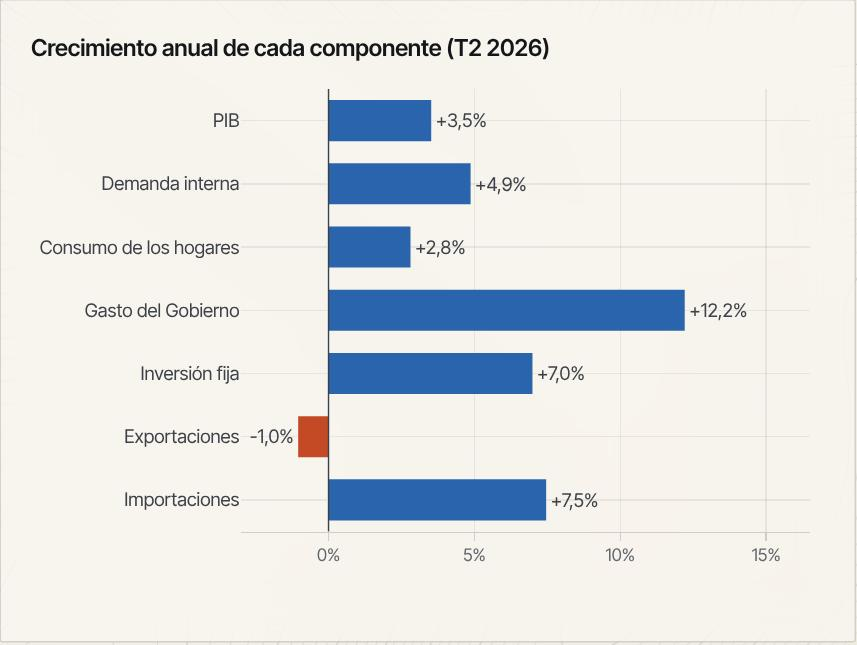
\includegraphics[width=\linewidth,height=0.42\textheight,keepaspectratio]{fig/g-demanda-crec.jpg}\end{center}
\paragraph{Qué nos cuenta}
Muestra cuánto creció en términos reales cada gran componente de la demanda en el último trimestre publicado: PIB, demanda interna, consumo de los hogares, gasto del Gobierno, inversión fija, exportaciones e importaciones. A diferencia del gráfico de aportes, aquí no se pondera por tamaño: se ve el ritmo propio de cada componente.

\begin{leer}[Cómo se lee]
Eje horizontal en \% de variación anual real frente al mismo trimestre del año anterior (volúmenes encadenados, datos originales). Barras azules: el componente crece; naranjas: cae; el valor está escrito al final de cada barra. El orden es fijo, de arriba abajo: PIB, demanda interna, consumo de los hogares (incluye las ISFLH), gasto del Gobierno, inversión fija, exportaciones e importaciones. La línea vertical marca el cero.
\end{leer}

\paragraph{Por qué importa}
Comparar la demanda interna con el PIB indica si el gasto de residentes va más rápido que la producción, lo que se cubre con importaciones y se refleja en la cuenta corriente. El ritmo de la inversión anticipa la ampliación de capacidad productiva y el de las exportaciones muestra la conexión con la demanda externa, datos relevantes para la tasa de cambio y las cuentas externas.

\paragraph{Cómo interpretarlo}
\begin{itemize}
\item Demanda interna por encima del PIB: el país gasta más rápido de lo que produce y la diferencia sale por importaciones; por debajo, ocurre lo contrario.
\item Las importaciones restan en la identidad del PIB: si crecen, una parte del gasto interno se atiende con producción extranjera.
\item La inversión fija es el componente más volátil: tasas de dos dígitos, positivas o negativas, son frecuentes y deben leerse junto con su nivel (ver la tasa de inversión).
\item Un solo trimestre puede estar afectado por calendario, revisiones o efectos base; el gráfico de aportes muestra la evolución en el tiempo.
\end{itemize}
\begin{formulas}[Fórmulas]
\formula{Variación anual real}{g\textsubscript{k,t} = (C\textsubscript{k,t} $\div$ C\textsubscript{k,t−4} − 1) $\times$ 100}{C\textsubscript{k,t} = volumen encadenado del componente k en el último trimestre t}
\formula{Identidad del gasto}{PIB = C\textsubscript{hog} + G + FBKF + $\Delta$E + X − M}{C\textsubscript{hog} = consumo de los hogares; G = Gobierno; FBKF = inversión fija; $\Delta$E = existencias; X − M = comercio neto (a precios corrientes; en volúmenes encadenados la suma no es exacta)}
\end{formulas}
\begin{metodo}[Metodología]
Variación anual de los volúmenes encadenados (datos originales) del último trimestre publicado. Consumo de los hogares incluye las ISFLH.
\par\smallskip{\small\textbf{Fuente:} DANE, PIB por el enfoque del gasto (anexos a precios constantes y corrientes)}
\end{metodo}

\section{¿Cuánto invierte el país?}

\subsection{Tasa de inversión: inversión fija como \% del PIB}
\label{g:g-tasa-inversion}
\begin{center}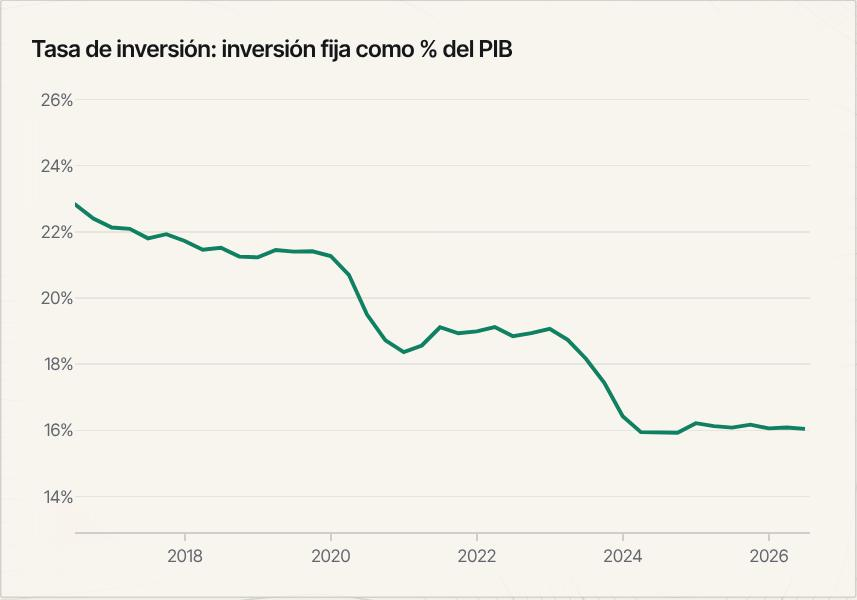
\includegraphics[width=\linewidth,height=0.42\textheight,keepaspectratio]{fig/g-tasa-inversion.jpg}\end{center}
\paragraph{Qué nos cuenta}
Mide qué parte de todo lo que produce el país se destina a inversión fija: construcción de vivienda y obras, maquinaria y equipo, y propiedad intelectual (software, investigación). Es la formación bruta de capital fijo (FBKF) como porcentaje del PIB, ambos en pesos corrientes y sumando los últimos 12 meses. Cuenta la historia del esfuerzo de inversión del país: su ascenso durante el auge de materias primas y su retroceso posterior.

\begin{leer}[Cómo se lee]
Eje vertical en \% del PIB, una sola línea verde con toda la historia disponible. Cada punto es el cociente entre la inversión fija y el PIB de los cuatro trimestres terminados en ese trimestre, a precios corrientes. La escala vertical se ajusta al rango de la serie, por lo que no empieza en cero: las variaciones se ven amplificadas. No incluye la variación de existencias (inventarios).
\end{leer}

\paragraph{Por qué importa}
La inversión de hoy es el capital con que se producirá en el futuro: una tasa de inversión baja limita el crecimiento potencial, la productividad y la generación de empleo de calidad. Para un inversionista, es un indicador estructural del atractivo y la confianza empresarial, y se vincula con la demanda de crédito, las importaciones de bienes de capital y la construcción.

\paragraph{Cómo interpretarlo}
\begin{itemize}
\item Una tasa que sube indica que una parte mayor del ingreso se dedica a ampliar capacidad; si baja de forma sostenida, la economía acumula menos capital.
\item Al estar en pesos corrientes, la tasa depende también de precios relativos: si los bienes de capital (muchos importados) se encarecen con la devaluación, la tasa puede subir sin más inversión real. El gráfico por tipo de activo muestra los volúmenes reales.
\item La suma de 12 meses elimina la estacionalidad pero hace que los giros aparezcan con algunos trimestres de rezago.
\item La tasa de inversión de Colombia se suele comparar con la de otras economías emergentes; las diferencias metodológicas entre países deben considerarse.
\end{itemize}
\begin{formulas}[Fórmulas]
\formula{Tasa de inversión}{TI\textsubscript{t} = ($\Sigma$\textsubscript{k=0..3} FBKF\textsubscript{t−k} $\div$ $\Sigma$\textsubscript{k=0..3} PIB\textsubscript{t−k}) $\times$ 100}{FBKF y PIB a precios corrientes (billones de pesos)}
\end{formulas}
\begin{metodo}[Metodología]
Formación bruta de capital fijo / PIB, ambos a precios corrientes y como suma de los últimos 4 trimestres. No incluye variación de existencias.
\par\smallskip{\small\textbf{Fuente:} DANE, PIB por el enfoque del gasto (anexos a precios constantes y corrientes)}
\end{metodo}

\subsection{Inversión por tipo de activo, T4 2019 = 100}
\label{g:g-inversion-activos}
\begin{center}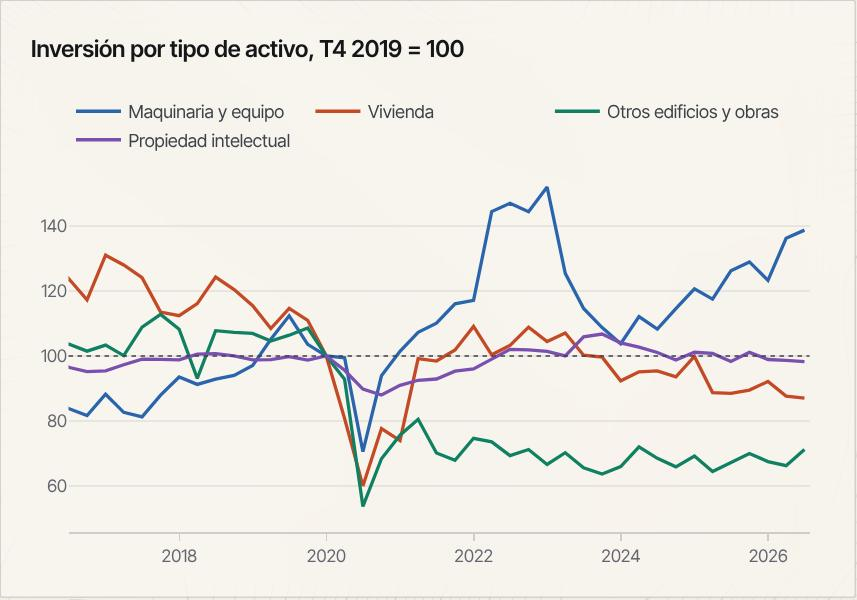
\includegraphics[width=\linewidth,height=0.42\textheight,keepaspectratio]{fig/g-inversion-activos.jpg}\end{center}
\paragraph{Qué nos cuenta}
Sigue el volumen real de la inversión fija por tipo de activo y lo compara con el nivel de finales de 2019, el último trimestre antes de la pandemia. Separa cuatro destinos: maquinaria y equipo, vivienda, otros edificios y obras civiles (carreteras, infraestructura, edificaciones no residenciales) y propiedad intelectual. Muestra qué tipos de inversión ya recuperaron su nivel previo y cuáles siguen rezagados.

\begin{leer}[Cómo se lee]
Eje vertical: índice con 2019T4 = 100, desde 2015. Línea azul: maquinaria y equipo (códigos AN113 + AN114 del Sistema de Cuentas Nacionales); naranja: vivienda (AN111); verde: otros edificios y obras (AN112); morada: propiedad intelectual (AN117). Todas son volúmenes desestacionalizados (cuadro 6 del anexo de gasto del DANE). La línea punteada en 100 es el nivel previo a la pandemia: por encima, el activo ya lo superó; por debajo, aún no.
\end{leer}

\paragraph{Por qué importa}
No toda la inversión tiene el mismo efecto: la maquinaria y la propiedad intelectual elevan la productividad, la vivienda atiende la demanda de los hogares y las obras civiles dependen en gran parte de la infraestructura pública y las concesiones. Saber cuál se recupera y cuál no ayuda a leer la capacidad productiva futura y el desempeño de sectores como construcción, cemento, importadores de bienes de capital y banca hipotecaria.

\paragraph{Cómo interpretarlo}
\begin{itemize}
\item Una línea que se mantiene por debajo de 100 indica que ese tipo de inversión aún no recupera el volumen previo a la pandemia; la distancia mide el rezago en \%.
\item La maquinaria y equipo es sensible a la tasa de cambio, porque buena parte se importa; la vivienda, a las tasas hipotecarias y a los subsidios; las obras civiles, a la ejecución pública.
\item El índice muestra el nivel relativo a una fecha, no el crecimiento anual; una línea que sube indica aumento del volumen, aunque siga por debajo de 100.
\item Las series desestacionalizadas se reestiman con cada publicación y pueden cambiar trimestres anteriores.
\end{itemize}
\begin{formulas}[Fórmulas]
\formula{Índice por activo}{I\textsubscript{j,t} = 100 $\times$ K\textsubscript{j,t} $\div$ K\textsubscript{j,2019T4}}{K\textsubscript{j,t} = formación bruta de capital fijo real desestacionalizada del activo j en el trimestre t}
\end{formulas}
\begin{metodo}[Metodología]
Cuadro 6 del anexo de gasto: formación bruta de capital fijo por tipo de activo (AN111 vivienda, AN112 otros edificios y estructuras, AN113+AN114 maquinaria y equipo, AN117 propiedad intelectual), volúmenes desestacionalizados; índice T4 2019 = 100.
\par\smallskip{\small\textbf{Fuente:} DANE, PIB por el enfoque del gasto (anexos a precios constantes y corrientes)}
\end{metodo}

\section{¿En qué gastan los hogares?}

\subsection{Consumo de los hogares por durabilidad, 12 meses}
\label{g:g-consumo-durabilidad}
\begin{center}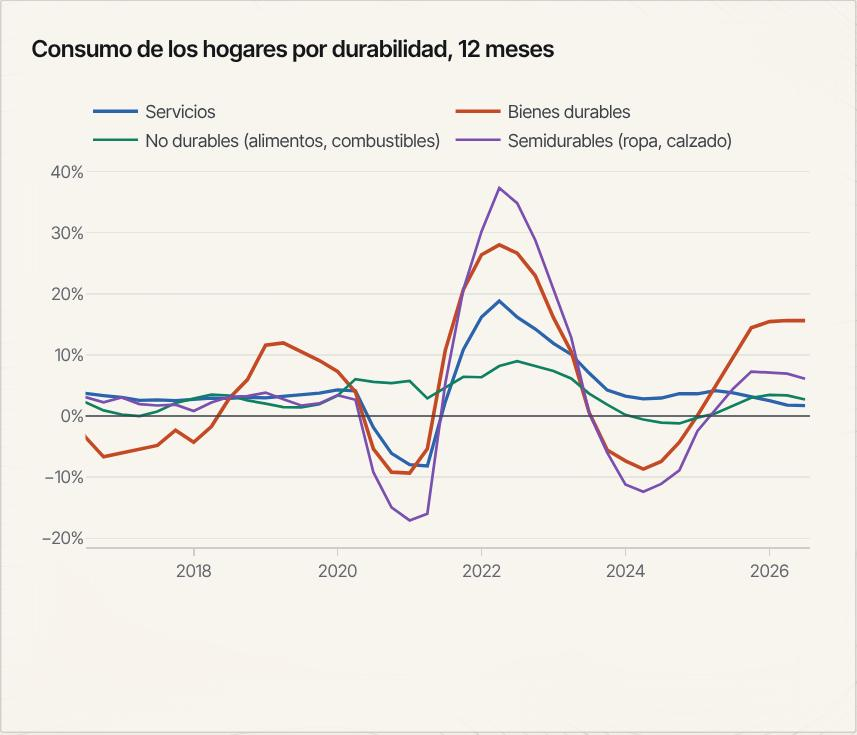
\includegraphics[width=\linewidth,height=0.42\textheight,keepaspectratio]{fig/g-consumo-durabilidad.jpg}\end{center}
\paragraph{Qué nos cuenta}
Divide el consumo de los hogares en cuatro tipos según su durabilidad: bienes durables (vehículos, electrodomésticos, muebles), semidurables (ropa, calzado), no durables (alimentos, combustibles) y servicios. Cada tipo responde de forma distinta al ciclo: los durables son los más sensibles al ingreso, al crédito y a la confianza, mientras que los no durables y los servicios básicos son más estables.

\begin{leer}[Cómo se lee]
Eje en \%, desde 2015. Cada línea es la variación real de los últimos 12 meses frente a los 12 anteriores (suma de cuatro trimestres, volúmenes en datos originales, cuadro 3 del anexo de gasto del DANE). Azul: servicios; naranja: bienes durables; verde: no durables; morada: semidurables. La línea en cero separa crecimiento de caída. Para conservar la escala, los valores se recortan entre −30\% y 40\%, lo que afecta sobre todo a 2020–2021.
\end{leer}

\paragraph{Por qué importa}
El consumo de los hogares es el componente más grande del PIB. Su composición revela la confianza de los hogares y el papel del crédito: un auge de durables suele ir de la mano de crédito de consumo y tasas bajas, y su caída es una de las primeras señales de enfriamiento. Para un inversionista es información directa sobre comercio, vehículos, bienes de consumo y la cartera de consumo de los bancos.

\paragraph{Cómo interpretarlo}
\begin{itemize}
\item Los durables oscilan mucho más que el resto: caídas de dos dígitos son habituales en desaceleraciones y alzas fuertes en recuperaciones.
\item Si los servicios crecen mientras los bienes se estancan, el consumo se está desplazando hacia actividades como restaurantes, turismo o entretenimiento.
\item La medida de 12 meses es suave y reacciona con rezago: un giro reciente tarda varios trimestres en reflejarse por completo.
\item Las tasas de política del Banco de la República y las de crédito de consumo (página de tasas) ayudan a interpretar el comportamiento de los durables.
\end{itemize}
\begin{formulas}[Fórmulas]
\formula{Variación de 12 meses}{g\textsubscript{12m,t} = ($\Sigma$\textsubscript{k=0..3} C\textsubscript{t−k} $\div$ $\Sigma$\textsubscript{k=4..7} C\textsubscript{t−k} − 1) $\times$ 100}{C = consumo real de los hogares del grupo de durabilidad (datos originales)}
\formula{Recorte gráfico}{valor dibujado = min(40; max(−30; g\textsubscript{12m}))}{afecta sobre todo a 2020–2021; el valor real puede ser más extremo}
\end{formulas}
\begin{metodo}[Metodología]
Cuadro 3: gasto de consumo final de los hogares en el territorio por durabilidad, volúmenes en datos originales; variación de la suma de 4 trimestres frente a los 4 anteriores.
\par\smallskip{\small\textbf{Fuente:} DANE, PIB por el enfoque del gasto (anexos a precios constantes y corrientes)}
\end{metodo}

\subsection{¿En qué gasta más (o menos) el hogar? 12 meses}
\label{g:g-consumo-finalidad}
\begin{center}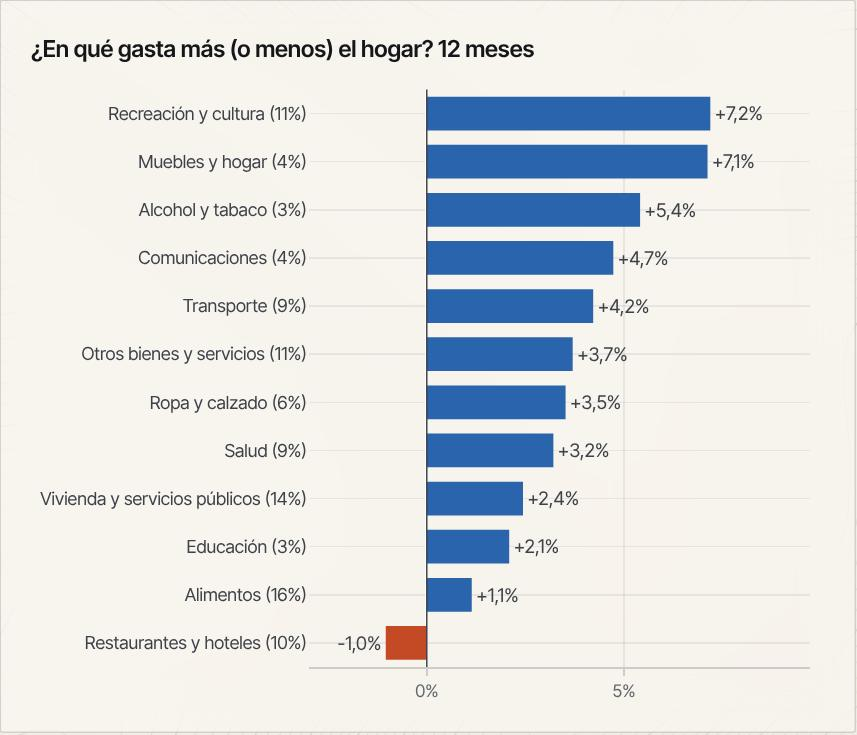
\includegraphics[width=\linewidth,height=0.42\textheight,keepaspectratio]{fig/g-consumo-finalidad.jpg}\end{center}
\paragraph{Qué nos cuenta}
Clasifica el gasto de los hogares según su finalidad, siguiendo la Clasificación del Consumo Individual por Finalidades (COICOP) de Naciones Unidas: alimentos, vivienda y servicios públicos, transporte, salud, educación, restaurantes y hoteles, entre otros, 12 grupos en total. Muestra en qué rubros los hogares están gastando más y en cuáles menos, en términos reales, durante el último año.

\begin{leer}[Cómo se lee]
Eje horizontal en \%: variación real de los últimos 12 meses frente a los 12 anteriores, con volúmenes en datos originales (cuadro 3 del anexo de gasto del DANE). Las barras están ordenadas de menor (abajo) a mayor (arriba) crecimiento; azul si crece y naranja si cae, con el valor escrito al final. Entre paréntesis, junto al nombre, la participación aproximada de cada grupo en el consumo total de los últimos 12 meses. La línea vertical marca el cero.
\end{leer}

\paragraph{Por qué importa}
La composición del gasto refleja prioridades y presiones de los hogares: si crecen sobre todo los rubros esenciales mientras caen los discrecionales, el consumo se está ajustando. Para un inversionista, la información orienta sobre sectores como comercio de alimentos, restaurantes, turismo, transporte o comunicaciones, y complementa la lectura de la inflación por grupos de gasto.

\paragraph{Cómo interpretarlo}
\begin{itemize}
\item Combine crecimiento y participación: un grupo con peso alto, como alimentos o vivienda, mueve mucho más el consumo total que uno pequeño que crece rápido.
\item Los rubros discrecionales (recreación, restaurantes y hoteles, muebles) suelen ser los primeros en ajustarse cuando el ingreso se debilita.
\item La participación se calcula con volúmenes encadenados, que no son aditivos: es una aproximación útil para ordenar, no un dato exacto.
\item Es una variación real: un rubro con precios al alza puede mostrar un gasto en pesos mayor y, aun así, un volumen menor.
\end{itemize}
\begin{formulas}[Fórmulas]
\formula{Variación de 12 meses}{g\textsubscript{j} = ($\Sigma$\textsubscript{k=0..3} C\textsubscript{j,t−k} $\div$ $\Sigma$\textsubscript{k=4..7} C\textsubscript{j,t−k} − 1) $\times$ 100}{C\textsubscript{j} = consumo real de los hogares en la finalidad COICOP j}
\formula{Participación aproximada}{s\textsubscript{j} = $\Sigma$\textsubscript{k=0..3} C\textsubscript{j,t−k} $\div$ $\Sigma$\textsubscript{i} $\Sigma$\textsubscript{k=0..3} C\textsubscript{i,t−k} $\times$ 100}{suma de volúmenes encadenados de los 12 grupos en los últimos 4 trimestres}
\end{formulas}
\begin{metodo}[Metodología]
Cuadro 3: consumo de los hogares por división COICOP (12 finalidades), volúmenes en datos originales; variación de 12 meses. La participación usa la suma de volúmenes encadenados (aproximada).
\par\smallskip{\small\textbf{Fuente:} DANE, PIB por el enfoque del gasto (anexos a precios constantes y corrientes)}
\end{metodo}

\section{¿Cuánto produce cada colombiano?}

\subsection{Crecimiento real del PIB por persona}
\label{g:g-pib-persona}
\begin{center}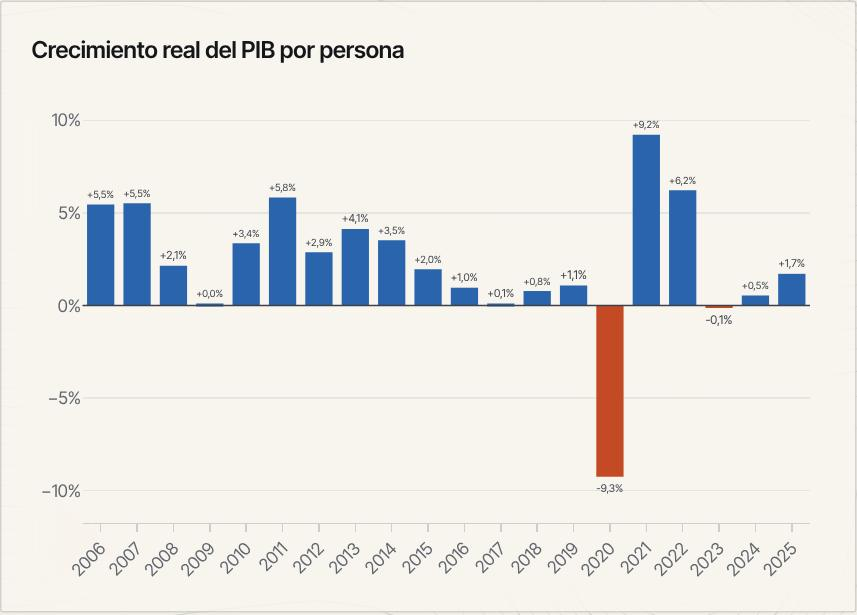
\includegraphics[width=\linewidth,height=0.42\textheight,keepaspectratio]{fig/g-pib-persona.jpg}\end{center}
\paragraph{Qué nos cuenta}
Mide cuánto creció la producción por habitante, descontando la inflación, en cada año calendario completo. Como la población también crece, el PIB por persona avanza menos que el PIB total: la diferencia es aproximadamente el crecimiento demográfico. Es la medida más directa de si el nivel de vida material promedio mejora o se estanca.

\begin{leer}[Cómo se lee]
Eje vertical en \%: crecimiento del PIB real por persona frente al año anterior. Cada barra es un año completo (solo años con sus cuatro trimestres publicados); azul si creció y naranja si cayó, con el valor encima. Al pasar el cursor se ve el nivel del PIB por persona en millones de pesos constantes de 2015. La línea horizontal marca el cero. La población es la total nacional a mitad de año según las estimaciones oficiales del DANE basadas en el Censo 2018.
\end{leer}

\paragraph{Por qué importa}
Un PIB que crece al mismo ritmo que la población deja el ingreso promedio estancado. Para comparar el progreso económico entre países o periodos, y para entender el potencial de consumo por habitante, el PIB por persona es más relevante que el total. También ayuda a separar el efecto del crecimiento demográfico, incluido el aporte de la migración, del avance genuino de la producción.

\paragraph{Cómo interpretarlo}
\begin{itemize}
\item La diferencia entre el crecimiento del PIB total y el del PIB por persona es aproximadamente la tasa de crecimiento de la población.
\item Cambios en las estimaciones de población del DANE modifican toda la serie por persona aunque el PIB no cambie; la actualización vigente reemplaza las anteriores.
\item El PIB por persona es un promedio: no informa sobre la distribución del ingreso ni sobre la informalidad.
\item Antes de 2018 la población es una retroestimación del DANE, consistente con el censo, pero sujeta a mayor incertidumbre.
\end{itemize}
\begin{formulas}[Fórmulas]
\formula{PIB real por persona}{y\textsubscript{A} = $\Sigma$\textsubscript{q$\in$A} Y\textsubscript{q} $\div$ P\textsubscript{A}}{Y\textsubscript{q} = PIB real del trimestre q (pesos de 2015); P\textsubscript{A} = población total nacional a mitad del año A}
\formula{Crecimiento anual}{g\textsubscript{A} = (y\textsubscript{A} $\div$ y\textsubscript{A−1} − 1) $\times$ 100}{y\textsubscript{A} = PIB real por persona del año A}
\formula{Descomposición aproximada}{g\textsubscript{y} $\approx$ g\textsubscript{PIB} − g\textsubscript{P}}{g\textsubscript{P} = crecimiento de la población}
\end{formulas}
\begin{metodo}[Metodología]
PIB real anual (suma de 4 trimestres, pesos de 2015) / población total nacional a 30 de junio. La población de 2018 en adelante es la proyección oficial vigente del DANE; antes de 2018, la retroproyección.
\par\smallskip{\small\textbf{Fuente:} DANE: PIB real y proyecciones de población (Censo 2018, actualización 2025); cálculo propio}
\end{metodo}

\subsection{PIB por persona en dólares}
\label{g:g-pib-persona-usd}
\begin{center}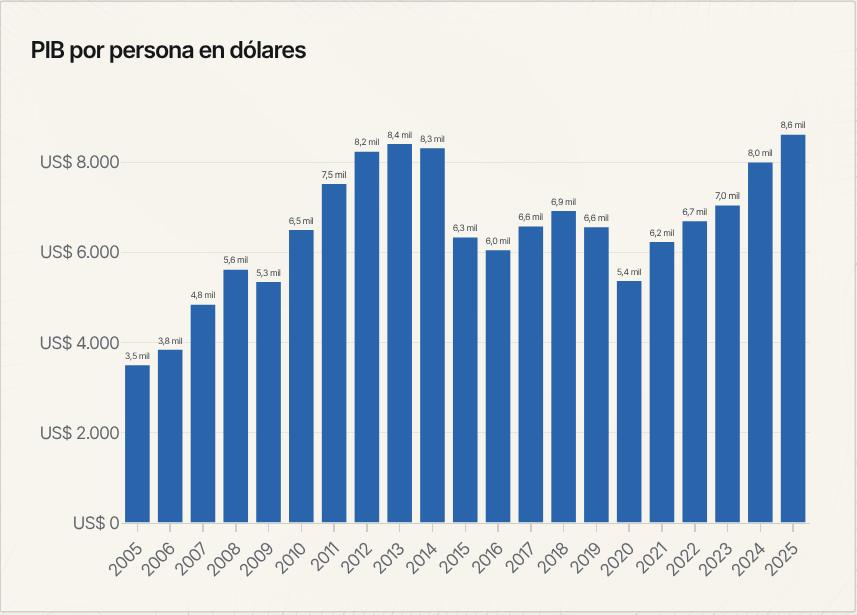
\includegraphics[width=\linewidth,height=0.42\textheight,keepaspectratio]{fig/g-pib-persona-usd.jpg}\end{center}
\paragraph{Qué nos cuenta}
Expresa el PIB por habitante en dólares corrientes, convirtiendo el PIB nominal en pesos con la tasa de cambio promedio de cada año. Es la cifra que suele usarse en comparaciones internacionales de ingreso. A diferencia del gráfico en pesos constantes, mezcla tres fuerzas: el crecimiento real, la inflación interna y el valor del peso frente al dólar.

\begin{leer}[Cómo se lee]
Eje vertical en dólares estadounidenses por persona; cada barra es un año calendario completo y su etiqueta muestra el valor en miles de dólares. El cálculo divide el PIB nominal anual (suma de cuatro trimestres, en pesos corrientes) entre la población a mitad de año y entre el promedio anual de la Tasa Representativa del Mercado (TRM), el tipo de cambio oficial peso-dólar que publica el Banco de la República. No se aplica el método Atlas del Banco Mundial.
\end{leer}

\paragraph{Por qué importa}
Para un inversionista extranjero, el PIB por persona en dólares aproxima el tamaño del mercado por consumidor en su propia moneda y el poder de compra internacional del país. Sus oscilaciones, sin embargo, dependen mucho de la tasa de cambio: años con devaluación fuerte muestran caídas en dólares aunque la economía crezca en términos reales.

\paragraph{Cómo interpretarlo}
\begin{itemize}
\item Si el dato en dólares cae mientras el PIB real por persona crece, la causa es la depreciación del peso; si sube más que el real, influyen la inflación y la apreciación.
\item No ajusta por paridad de poder adquisitivo (PPA): no refleja que en Colombia muchos bienes y servicios son más baratos que en EE. UU.
\item Como usa la TRM promedio del año, una devaluación concentrada al final del año se refleja solo en parte.
\item Compárelo con el crecimiento real por persona y con la página de la tasa de cambio para separar las tres fuerzas.
\end{itemize}
\begin{formulas}[Fórmulas]
\formula{PIB por persona en dólares}{PIB\textsubscript{USD,A} = $\Sigma$\textsubscript{q$\in$A} N\textsubscript{q} $\div$ P\textsubscript{A} $\div$ TR$\bar{\mathrm{M}}$\textsubscript{A}}{N = PIB nominal en pesos; P = población a mitad de año; TR$\bar{\mathrm{M}}$ = promedio de la TRM diaria del año calendario}
\formula{Descomposición aproximada}{$\Delta$\% PIB\textsubscript{USD} $\approx$ g\textsubscript{real por persona} + $\pi$\textsubscript{deflactor} − $\Delta$\% TR$\bar{\mathrm{M}}$}{en tasas anuales; aproximación de primer orden}
\end{formulas}
\begin{metodo}[Metodología]
PIB nominal anual / población / TRM promedio del año calendario. Método Atlas no aplicado: es la conversión simple a la tasa de mercado.
\par\smallskip{\small\textbf{Fuente:} DANE (PIB nominal, población) y Banco de la República (TRM); cálculo propio}
\end{metodo}

\subsection{Producción, empleo y producción por ocupado, 2015 = 100}
\label{g:g-productividad}
\begin{center}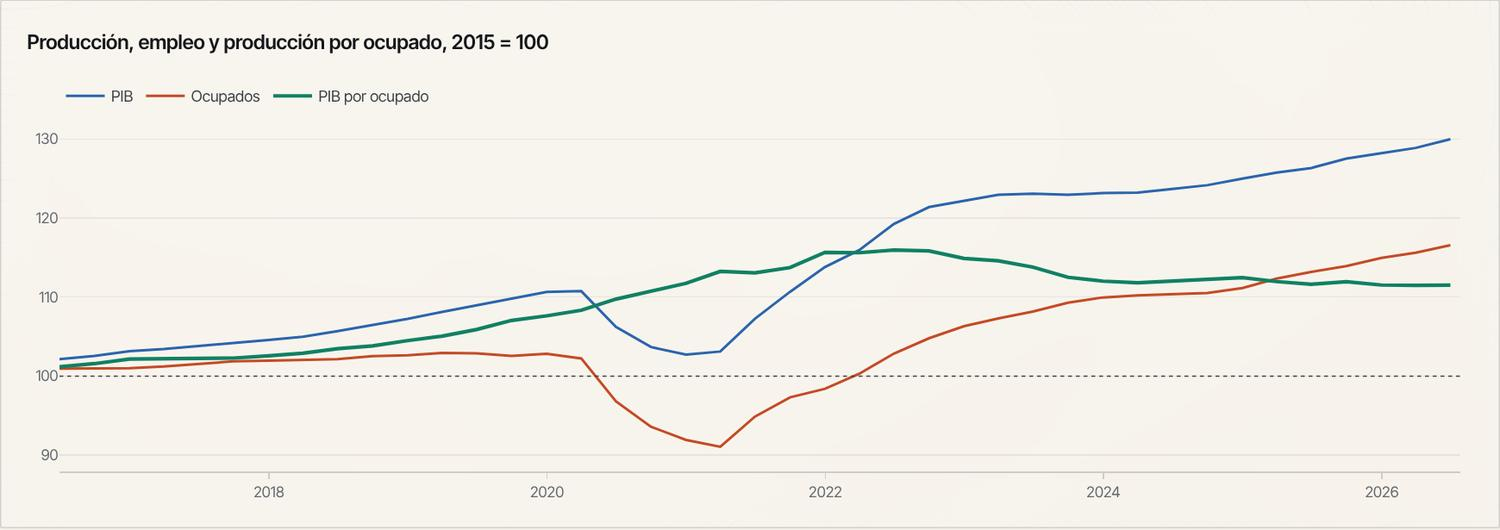
\includegraphics[width=\linewidth,height=0.42\textheight,keepaspectratio]{fig/g-productividad.jpg}\end{center}
\paragraph{Qué nos cuenta}
Compara la evolución de la producción y del empleo y, a partir de ambas, la producción por persona ocupada, llamada productividad laboral aparente (OCDE, 2001). Si el PIB crece más que el número de ocupados, cada trabajador produce en promedio más; si el empleo crece más rápido que la producción, la productividad por ocupado cae. Es una lectura directa de la eficiencia con que la economía usa su fuerza laboral.

\begin{leer}[Cómo se lee]
Eje vertical: índices con promedio de 2015 = 100, desde 2015. Línea azul: PIB real de los últimos 12 meses (suma de cuatro trimestres). Línea naranja: ocupados, promedio de 12 meses de la Gran Encuesta Integrada de Hogares (GEIH) del DANE, serie desestacionalizada. Línea verde, más gruesa: el cociente entre ambos, PIB por ocupado. La línea punteada en 100 es el nivel promedio de 2015.
\end{leer}

\paragraph{Por qué importa}
La productividad es el determinante de largo plazo de los salarios reales y del crecimiento potencial: sin ella, el PIB solo crece si crece el empleo. Para un inversionista, una productividad estancada limita el margen para subir salarios sin presionar costos, y una productividad al alza sostiene la rentabilidad y la competitividad externa.

\paragraph{Cómo interpretarlo}
\begin{itemize}
\item Verde al alza: la producción crece más que el empleo; verde a la baja: el empleo crece más rápido que la producción, algo frecuente cuando se crean puestos en actividades de baja productividad.
\item Es productividad aparente: no corrige por horas trabajadas, por informalidad ni por el capital disponible, de modo que mezcla eficiencia con composición del empleo.
\item Los cambios metodológicos o de marco muestral de la GEIH pueden generar saltos en los ocupados que no reflejan cambios económicos.
\item Compárela con la página de empleo y con el crecimiento por sector para ver qué actividades explican los movimientos.
\end{itemize}
\begin{formulas}[Fórmulas]
\formula{Índice del PIB}{I\textsuperscript{Y}\textsubscript{t} = 100 $\times$ Y\textsuperscript{4}\textsubscript{t} $\div$ $\bar{Y}$\textsuperscript{4}\textsubscript{2015}}{Y\textsuperscript{4}\textsubscript{t} = suma del PIB real de los trimestres t−3 a t; $\bar{Y}$\textsuperscript{4}\textsubscript{2015} = promedio de esa suma en 2015}
\formula{Índice de ocupados}{I\textsuperscript{E}\textsubscript{t} = 100 $\times$ E\textsuperscript{12}\textsubscript{t} $\div$ Ē\textsuperscript{12}\textsubscript{2015}}{E\textsuperscript{12}\textsubscript{t} = promedio de ocupados desestacionalizados de los últimos 12 meses}
\formula{PIB por ocupado}{I\textsuperscript{P}\textsubscript{t} = 100 $\times$ I\textsuperscript{Y}\textsubscript{t} $\div$ I\textsuperscript{E}\textsubscript{t}}{productividad laboral aparente, 2015 = 100}
\end{formulas}
\begin{metodo}[Metodología]
Productividad laboral aparente (OECD, 2001) = PIB real de 4 trimestres / promedio de ocupados de 12 meses; índices 2015 = 100. No corrige por horas trabajadas ni por informalidad.
\par\smallskip{\small\textbf{Fuente:} DANE: PIB real y GEIH desestacionalizada (población ocupada); cálculo propio}
\end{metodo}

\section{¿Dónde está la economía frente a su camino previo?}

\subsection{Nivel del PIB frente al camino de 2015–2019}
\label{g:g-nivel}
\begin{center}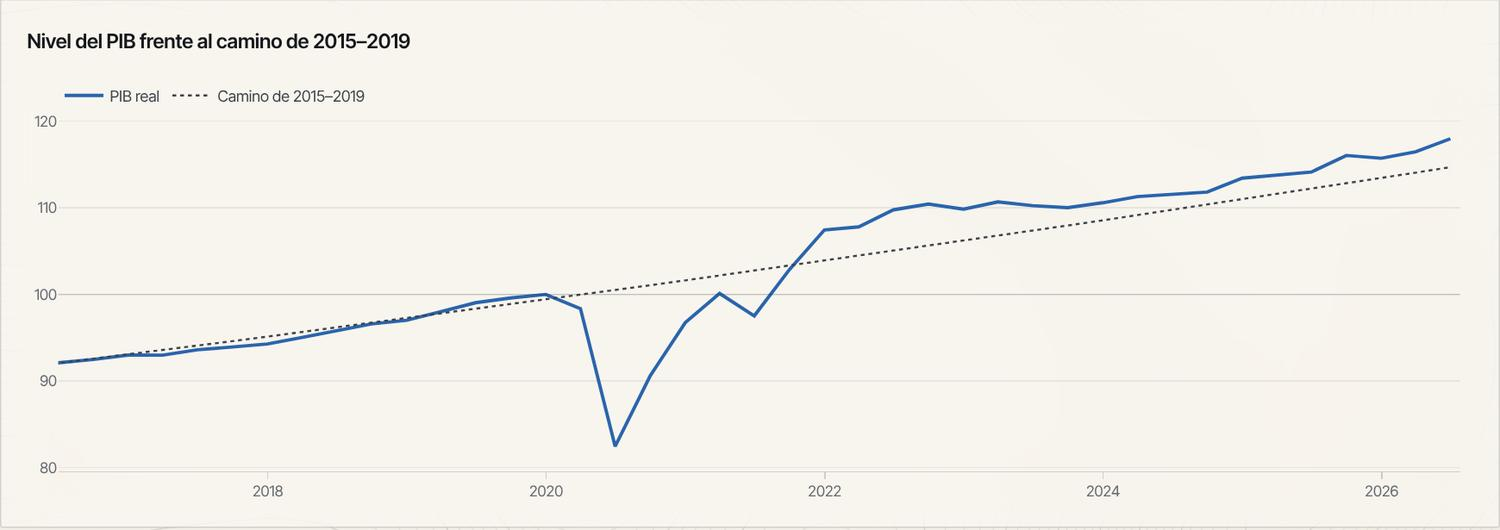
\includegraphics[width=\linewidth,height=0.42\textheight,keepaspectratio]{fig/g-nivel.jpg}\end{center}
\paragraph{Qué nos cuenta}
Compara el tamaño de la economía con el que habría tenido si hubiera mantenido el ritmo de crecimiento de 2015–2019. No mira tasas sino niveles: aunque la economía haya vuelto a crecer después de 2020, puede seguir por debajo del camino que traía, es decir, con una pérdida permanente de producción. La literatura sobre crisis (Cerra y Saxena, 2008) documenta que estas pérdidas de nivel son frecuentes.

\begin{leer}[Cómo se lee]
Eje vertical: índice del PIB real desestacionalizado con 2019T4 = 100, desde 2015. Línea azul: PIB observado. Línea gris punteada: camino de 2015–2019, una tendencia log-lineal ajustada a esos 20 trimestres y extendida con la misma pendiente; es un contrafactual descriptivo, no una estimación de lo que vendrá. La línea horizontal en 100 marca el tamaño de la economía antes de la pandemia.
\end{leer}

\paragraph{Por qué importa}
Las tasas de crecimiento altas tras una crisis pueden ocultar que la economía no ha recuperado lo perdido. La distancia frente al camino previo resume cuánta producción, ingreso y empleo dejó de generarse, y es relevante para evaluar el tamaño del mercado, la sostenibilidad fiscal y la discusión sobre si la capacidad productiva se redujo de forma duradera (histéresis).

\paragraph{Cómo interpretarlo}
\begin{itemize}
\item Azul por debajo de la línea punteada: la economía es más pequeña de lo que habría sido con el ritmo previo; la distancia, en \%, es la pérdida de nivel. Por encima: ya superó ese camino.
\item Que la azul esté sobre 100 solo indica que la economía es mayor que a finales de 2019, no que haya recuperado su tendencia.
\item El camino depende del periodo elegido: 2015–2019 incluye la desaceleración tras la caída del petróleo; con otro periodo, la pendiente y la brecha serían diferentes.
\item Las revisiones del DANE y del ajuste estacional pueden mover tanto el índice como la pendiente estimada.
\end{itemize}
\begin{formulas}[Fórmulas]
\formula{Índice del PIB}{I\textsubscript{t} = 100 $\times$ S\textsubscript{t} $\div$ S\textsubscript{2019T4}}{S = PIB real desestacionalizado}
\formula{Tendencia 2015–2019}{ln S\textsubscript{t} = b\textsubscript{0} + b\textsubscript{1} $\times$ k + $\varepsilon$\textsubscript{t};  Ŝ\textsubscript{k} = e\textsuperscript{b\textsubscript{0} + b\textsubscript{1} $\times$ k}}{k = 0, 1, 2… trimestres desde 2015T1; b\textsubscript{0}, b\textsubscript{1} por mínimos cuadrados con 2015T1–2019T4}
\formula{Ritmo anual del camino}{g\textsubscript{tend} = (e\textsuperscript{4 $\times$ b\textsubscript{1}} − 1) $\times$ 100}{crecimiento anual implícito en la pendiente trimestral}
\formula{Distancia al camino}{B\textsubscript{t} = (S\textsubscript{t} $\div$ Ŝ\textsubscript{t} − 1) $\times$ 100}{negativa: nivel por debajo del camino previo}
\end{formulas}
\begin{metodo}[Metodología]
Índice T4 2019 = 100. Camino previo: regresión log-lineal del PIB desestacionalizado de 2015T1–2019T4, prolongada con la misma pendiente. Es un contrafactual descriptivo, no un pronóstico. Ver Cerra y Saxena (2008) sobre pérdidas permanentes de nivel tras las crisis.
\par\smallskip{\small\textbf{Fuente:} DANE, PIB real desestacionalizado; cálculo propio}
\end{metodo}

\section*{Lecturas de la página}
\begin{itemize}\small
\item \textbf{Burns, A. F. y Mitchell, W. C. (1946). Measuring Business Cycles. NBER.} Índices de difusión: cuántos sectores se mueven en la misma dirección.
\item \textbf{Hodrick, R. J. y Prescott, E. C. (1997). Postwar U.S. Business Cycles. Journal of Money, Credit and Banking, 29(1), 1–16.} Tendencia y ritmo normal de crecimiento.
\item \textbf{Hamilton, J. D. (2018). Why You Should Never Use the Hodrick-Prescott Filter. Review of Economics and Statistics, 100(5), 831–843.} Crítica y alternativa al filtro HP (se usa en la página del ciclo).
\item \textbf{Kohli, U. (2004). Real GDP, Real Domestic Income, and Terms-of-Trade Changes. Journal of International Economics, 62(1), 83–106.} Por qué el deflactor del PIB y el IPC divergen cuando cambian los términos de intercambio.
\item \textbf{Cerra, V. y Saxena, S. C. (2008). Growth Dynamics: The Myth of Economic Recovery. American Economic Review, 98(1), 439–457.} Las crisis dejan pérdidas permanentes de nivel del producto.
\item \textbf{Blanchard, O., Cerutti, E. y Summers, L. (2015). Inflation and Activity: Two Explorations and their Monetary Policy Implications. IMF WP/15/230.} Histéresis: recesiones que reducen el camino del producto.
\item \textbf{DANE. Cuentas nacionales trimestrales: metodología (enfoque de la producción, índices encadenados).} Por qué los aportes por sector no suman exactamente el PIB (impuestos y encadenamiento).
\item \textbf{OECD (2001). Measuring Productivity: OECD Manual. París: OECD.} Productividad laboral aparente: producción por persona ocupada.
\item \textbf{Naciones Unidas et al. (2009). System of National Accounts 2008. Nueva York.} Enfoque del gasto, formación bruta de capital y consumo por finalidad (COICOP).
\item \textbf{DANE. Proyecciones y retroproyecciones de población, Censo Nacional de Población y Vivienda 2018 (actualización 2025).} Denominador del PIB por persona.
\end{itemize}

\chapter{Capacidad}
\label{atlas:capacidad}

{\large\sffamily\bfseries Capacidad productiva: sectores, trabajo y regiones\par}\medskip

Si la economía produce por encima o por debajo de lo que puede sostener sin generar inflación, y dónde: en qué sectores, en el mercado laboral y en cada departamento.

{\small\color{cmmuted}Página del sitio: \url{https://stv-quant.github.io/ColombiaMacro-USBCali/capacidad/}}

\section{¿Produce la economía por encima o por debajo de su capacidad?}

\subsection{Lo que produce la economía frente a su capacidad}
\label{g:g-capacidad}
\begin{center}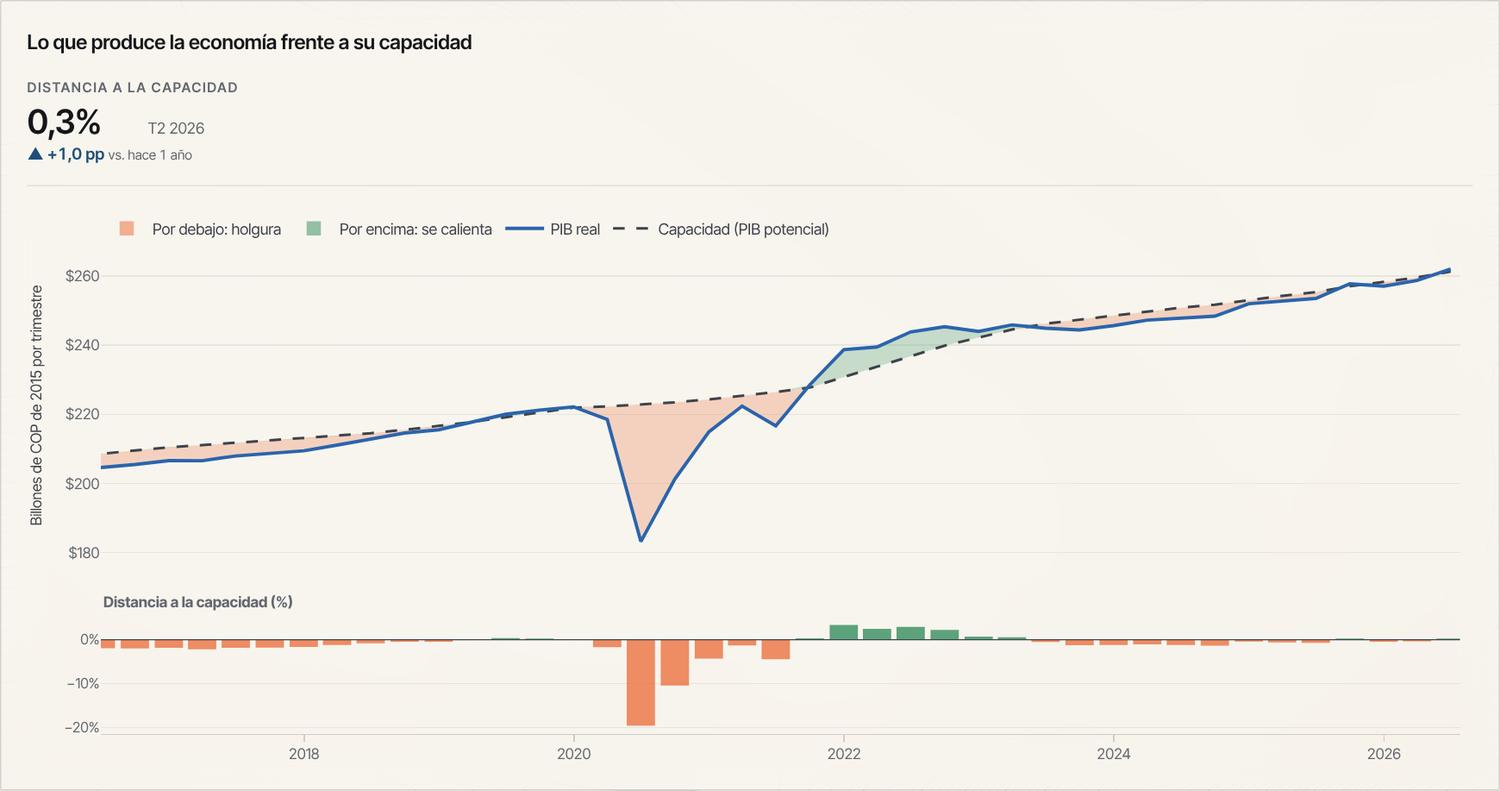
\includegraphics[width=\linewidth,height=0.42\textheight,keepaspectratio]{fig/g-capacidad.jpg}\end{center}
\paragraph{Qué nos cuenta}
Compara lo que la economía colombiana produce cada trimestre (PIB real desestacionalizado) con su capacidad, es decir, el PIB potencial: el nivel que puede sostener sin generar presiones de inflación. La distancia entre ambos es la brecha del producto, el termómetro central del ciclo: dice si la economía está recalentada o si tiene capacidad ociosa.

\begin{leer}[Cómo se lee]
Panel superior: la línea azul es el PIB real y la línea gris discontinua la capacidad, en billones de pesos de 2015 por trimestre (eje izquierdo). El área verde aparece cuando el PIB supera la capacidad y la naranja cuando queda por debajo. Panel inferior: barras con la brecha en porcentaje, verdes si es positiva y naranjas si es negativa, con una línea en cero. La vista inicial muestra los últimos diez años; la serie de brecha empieza cinco años después del primer dato del PIB, porque el filtro necesita al menos 20 trimestres.
\end{leer}

\paragraph{Por qué importa}
La brecha resume el balance entre demanda y oferta. Una brecha positiva suele acompañar presiones de precios y un mercado laboral apretado, y es una de las variables que el Banco de la República (BanRep) sigue para fijar su tasa de política monetaria (TPM). Para un inversionista, ubicar la economía frente a su capacidad ayuda a leer el contexto de inflación, tasas y utilidades empresariales.

\paragraph{Cómo interpretarlo}
\begin{itemize}
\item Brecha positiva: la economía produce por encima de lo sostenible; negativa: hay holgura (capacidad ociosa, desempleo). Valores entre −0,5\% y +0,5\% se leen como cercanos al potencial.
\item El potencial no se observa: se estima. Este gráfico usa un filtro Hodrick-Prescott (HP) en tiempo real, que en cada trimestre solo usa la información disponible hasta ese momento, para no reescribir la historia con datos posteriores.
\item El colapso de 2020 aparece como una brecha muy negativa; los trimestres 2020T2–2021T2 se excluyen al estimar la tendencia para que el choque no deforme la capacidad.
\item El último dato del PIB se revisa en publicaciones siguientes y el filtro es menos preciso al final de la muestra: conviene contrastar con la página Ciclo, donde la brecha se mide con cinco métodos.
\end{itemize}
\begin{formulas}[Fórmulas]
\formula{Brecha del producto}{brecha\textsubscript{t} = 100 $\times$ (ln Y\textsubscript{t} − ln Y*\textsubscript{t})}{Y = PIB real desestacionalizado del trimestre t; Y* = capacidad (tendencia HP en tiempo real)}
\formula{Filtro HP en tiempo real}{Y*\textsubscript{t} = último punto de $\tau$ que minimiza $\Sigma$\textsubscript{s$\le$t}(y\textsubscript{s} − $\tau$\textsubscript{s})\textsuperscript{2} + $\lambda$ $\Sigma$($\Delta$\textsuperscript{2}$\tau$\textsubscript{s})\textsuperscript{2}}{y = 100 $\times$ ln PIB; $\tau$ = tendencia; $\lambda$ = 1.600 (trimestral); solo datos hasta t; 2020T2–2021T2 interpolados}
\formula{Capacidad en pesos}{Y*\textsubscript{t} = Y\textsubscript{t} $\times$ e\textsuperscript{−brecha\textsubscript{t} $\div$ 100}}{convierte la brecha en el nivel de capacidad graficado (billones de COP de 2015)}
\end{formulas}
\begin{metodo}[Metodología]
Capacidad (PIB potencial) = tendencia del PIB estimada con un filtro de Hodrick-Prescott en tiempo real ($\lambda$ = 1.600, una cola: cada trimestre solo usa datos disponibles hasta ese momento), excluyendo el choque de 2020T2–2021T2. Brecha = 100 $\times$ (ln PIB − ln capacidad). Como contraste se calculan también un HP de dos colas y el método de Hamilton (2018); los tres coinciden en el signo casi siempre. Valores en billones de COP (pesos colombianos) de 2015 por trimestre.
\par\smallskip{\small\textbf{Fuente:} DANE, PIB real desestacionalizado (Cuadro 4); cálculo propio de la capacidad}
\end{metodo}

\section{¿Qué sectores trabajan por encima o por debajo de su capacidad?}

\subsection{Brecha de cada sector frente a su tendencia}
\label{g:g-cap-sectores}
\begin{center}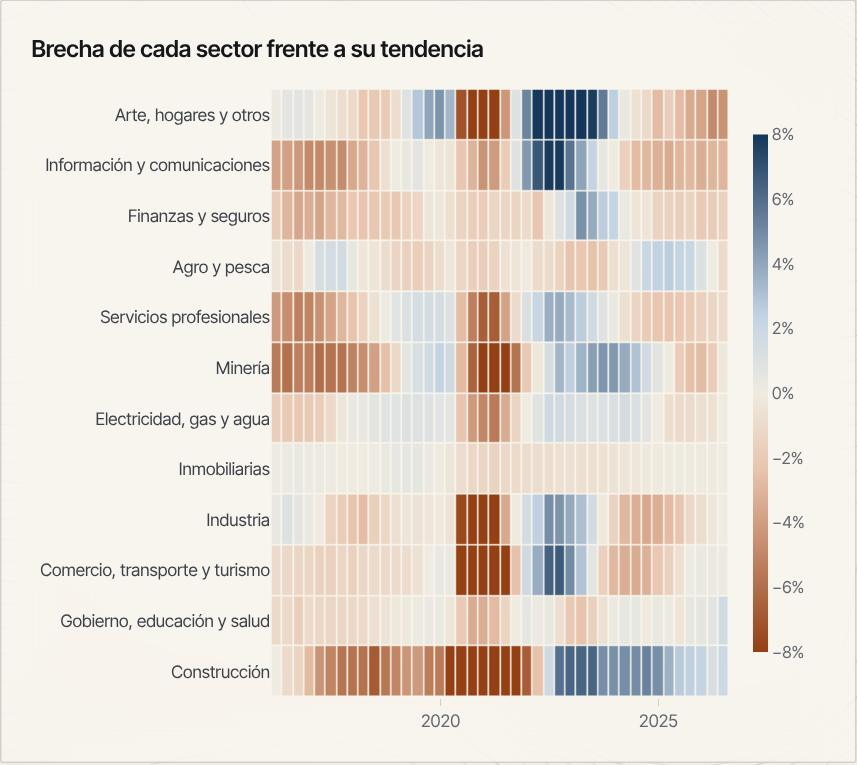
\includegraphics[width=\linewidth,height=0.42\textheight,keepaspectratio]{fig/g-cap-sectores.jpg}\end{center}
\paragraph{Qué nos cuenta}
Muestra, trimestre a trimestre, si cada una de las 12 grandes ramas de actividad de las cuentas nacionales produce por encima o por debajo de su propia tendencia. Permite ver si la holgura o el recalentamiento de la economía es general o se concentra en unos pocos sectores, y cómo ha cambiado ese mapa en el tiempo.

\begin{leer}[Cómo se lee]
Cada fila es un sector y cada columna un trimestre, desde 2016. El color es la brecha del sector en porcentaje: azul cuando produce por encima de su tendencia, naranja cuando produce por debajo y casi blanco cuando está cerca de ella. La escala de color va de −8\% a +8\%; valores más extremos (como los de 2020) se muestran con el color del límite. Las filas están ordenadas según la brecha del último trimestre. Al pasar el cursor se ve el valor exacto.
\end{leer}

\paragraph{Por qué importa}
Una brecha agregada positiva puede esconder sectores con mucha holgura. Saber dónde está la presión sirve para entender qué precios y qué mercados laborales se tensan, y qué ramas tienen espacio para crecer sin cuellos de botella. Para un inversionista, es una lectura del momento cíclico de cada industria.

\paragraph{Cómo interpretarlo}
\begin{itemize}
\item Columnas mayoritariamente azules indican una expansión generalizada; una mezcla de azules y naranjas, un ciclo desigual entre sectores.
\item Un sector que pasa de naranja a azul ha cerrado su holgura; el cambio inverso señala pérdida de dinamismo frente a su propia historia.
\item Los niveles sectoriales del DANE vienen sin desestacionalizar: se usa la suma de 4 trimestres, que elimina la estacionalidad, antes de filtrar. Eso suaviza la serie y hace que los giros aparezcan con algo de rezago.
\item Cada brecha se mide contra la tendencia del propio sector (no contra la economía): un sector en declive estructural puede verse cerca de cero aunque se contraiga. Complementa al gráfico de barras contiguo y a la casilla de amplitud de la página Ciclo.
\end{itemize}
\begin{formulas}[Fórmulas]
\formula{Nivel anualizado}{N\textsubscript{i,t} = $\Sigma$\textsubscript{k=0..3} X\textsubscript{i,t−k}}{X = valor agregado real trimestral (datos originales) del sector i}
\formula{Brecha sectorial}{b\textsubscript{i,t} = 100 $\times$ (ln N\textsubscript{i,t} − ln T\textsubscript{i,t})}{T = tendencia HP en tiempo real ($\lambda$ = 1.600, solo datos hasta t, 2020T2–2021T2 interpolados)}
\end{formulas}
\begin{metodo}[Metodología]
Brecha = 100 $\times$ (ln nivel real − ln tendencia), con tendencia Hodrick-Prescott de una cola ($\lambda$ = 1.600) calculada sin 2020T2–2021T2: en cada trimestre solo usa datos disponibles hasta ese momento.
\par\smallskip{\small\textbf{Fuente:} DANE, PIB trimestral por actividad; cálculo propio}
\end{metodo}

\subsection{Brecha de cada sector hoy (T2 2026)}
\label{g:g-cap-sectores-hoy}
\begin{center}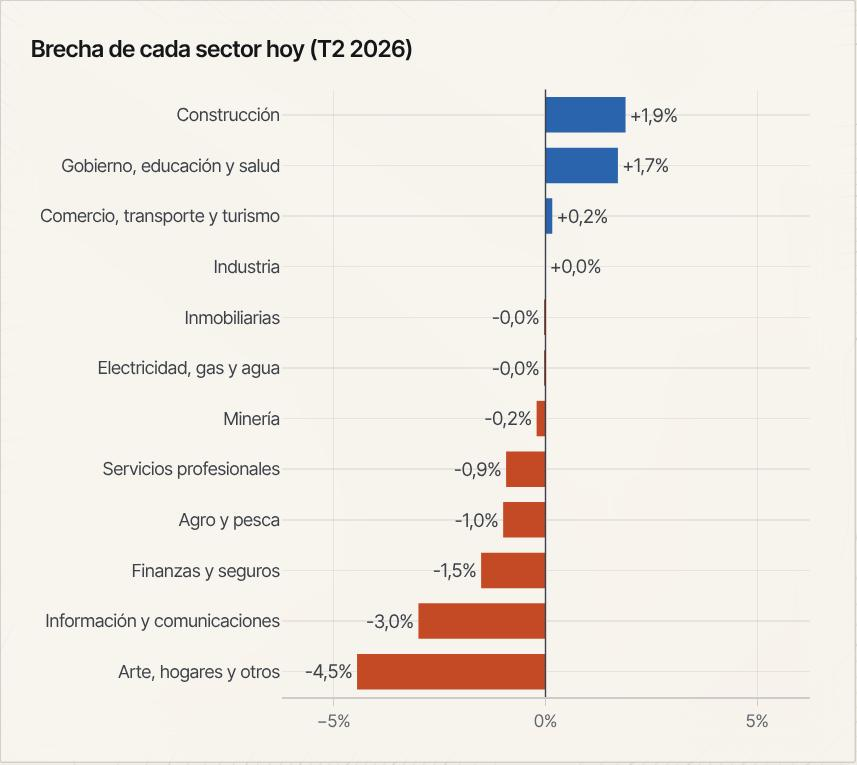
\includegraphics[width=\linewidth,height=0.42\textheight,keepaspectratio]{fig/g-cap-sectores-hoy.jpg}\end{center}
\paragraph{Qué nos cuenta}
Es la última columna del mapa de calor de sectores, presentada como ranking: la distancia porcentual entre lo que produce cada una de las 12 ramas en el trimestre más reciente y su tendencia. Muestra de un vistazo qué sectores trabajan sin holgura y cuáles tienen capacidad disponible.

\begin{leer}[Cómo se lee]
Barras horizontales, una por sector, con la brecha en porcentaje sobre el eje horizontal y el valor escrito al final de cada barra. Azul: el sector produce por encima de su tendencia; naranja: por debajo. La línea vertical marca el cero. Los sectores están ordenados de mayor brecha (arriba) a menor (abajo) y el eje es simétrico alrededor de cero.
\end{leer}

\paragraph{Por qué importa}
Cuando pocos sectores están por encima de su tendencia, el crecimiento puede convivir con presiones de precios acotadas; cuando la mayoría lo está, la presión tiende a ser más general. El ranking también identifica las ramas que hoy jalonan o frenan la actividad, útil para leer la exposición sectorial de empresas y carteras.

\paragraph{Cómo interpretarlo}
\begin{itemize}
\item Barras azules largas: sectores con poca holgura, donde pueden aparecer cuellos de botella o presiones de costos.
\item Barras naranjas: producción por debajo de la tendencia del propio sector; no implica necesariamente caída anual, sino menor ritmo que su historia.
\item El número de barras azules es el mismo que la casilla de amplitud («sectores sobre su tendencia») de la página Ciclo.
\item El dato del último trimestre es el más expuesto a revisiones del DANE y al sesgo de fin de muestra del filtro.
\end{itemize}
\begin{formulas}[Fórmulas]
\formula{Brecha sectorial}{b\textsubscript{i,T} = 100 $\times$ (ln N\textsubscript{i,T} − ln T\textsubscript{i,T})}{N = suma de 4 trimestres del valor agregado real del sector i; T = tendencia HP en tiempo real ($\lambda$ = 1.600); T = último trimestre}
\end{formulas}
\begin{metodo}[Metodología]
Último trimestre de la brecha de cada sector frente a su tendencia HP de una cola.
\par\smallskip{\small\textbf{Fuente:} DANE, PIB trimestral por actividad; cálculo propio}
\end{metodo}

\section{¿Cuánta holgura hay en el mercado laboral?}

\subsection{Desempleo, subempleo y subutilización total (promedio de 12 meses)}
\label{g:g-cap-subutilizacion}
\begin{center}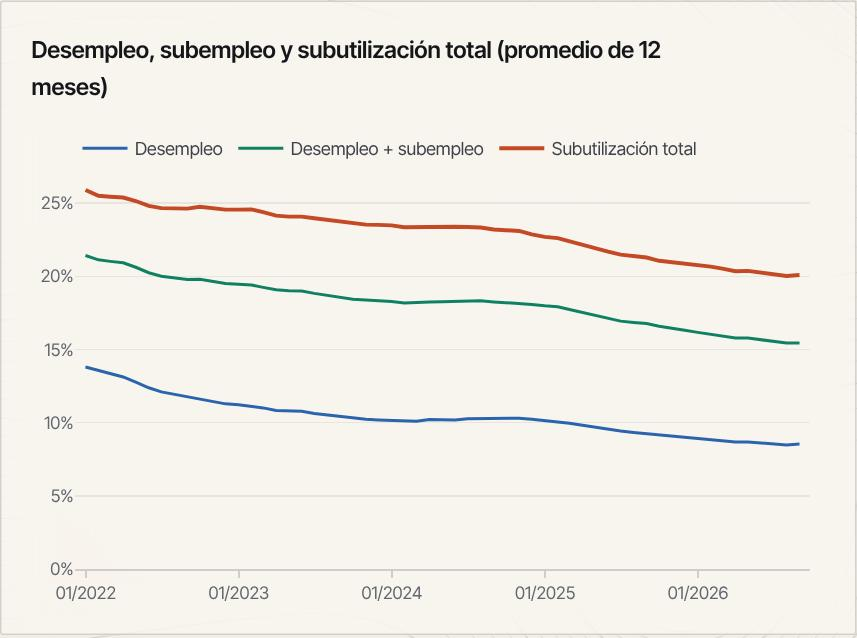
\includegraphics[width=\linewidth,height=0.42\textheight,keepaspectratio]{fig/g-cap-subutilizacion.jpg}\end{center}
\paragraph{Qué nos cuenta}
Mide la holgura del mercado laboral con tres indicadores de la Organización Internacional del Trabajo (OIT), del más estrecho al más amplio. La tasa de desempleo solo cuenta a quienes buscan empleo y no lo tienen; las otras dos suman a quienes trabajan menos horas de las que quieren y a quienes quieren trabajar pero no buscan.

\begin{leer}[Cómo se lee]
Tres líneas mensuales, cada una como promedio móvil de 12 meses, en porcentaje: azul, tasa de desempleo (TD); verde, desempleo más subempleo por horas (TCSD); naranja y más gruesa, la medida compuesta de subutilización (MCSFT), que agrega la fuerza de trabajo potencial. El eje vertical parte de cero. Datos del total nacional de la Gran Encuesta Integrada de Hogares (GEIH) del DANE, sin desestacionalizar.
\end{leer}

\paragraph{Por qué importa}
El desempleo por sí solo subestima la holgura cuando muchas personas trabajan pocas horas o se desaniman y dejan de buscar. Las medidas amplias dan una visión más completa del espacio que tiene la economía para crecer sin presionar los salarios, algo que pesa en la lectura de inflación y de política monetaria.

\paragraph{Cómo interpretarlo}
\begin{itemize}
\item Si la distancia entre la línea naranja y la azul crece, la holgura oculta (subempleo y desaliento) aumenta aunque el desempleo no cambie.
\item Las tres medidas bajando juntas indican un mercado laboral que absorbe trabajadores de forma amplia.
\item El promedio de 12 meses elimina la estacionalidad y el ruido de la encuesta, pero hace que los giros se vean con rezago; por eso la TD de este gráfico no coincide con la tasa desestacionalizada mensual que se usa en otras páginas.
\item La MCSFT usa un denominador distinto (fuerza de trabajo ampliada), así que no es la suma simple de las otras dos tasas.
\end{itemize}
\begin{formulas}[Fórmulas]
\formula{Tasa de desempleo}{TD = D $\div$ FT $\times$ 100}{D = desocupados; FT = fuerza de trabajo (ocupados + desocupados)}
\formula{Desempleo + subempleo}{TCSD = (D + S) $\div$ FT $\times$ 100}{S = subocupados por insuficiencia de horas}
\formula{Medida compuesta}{MCSFT = (D + S + FTP) $\div$ (FT + FTP) $\times$ 100}{FTP = fuerza de trabajo potencial: personas disponibles que quieren trabajar pero no buscan}
\formula{Promedio móvil}{$\bar{x}$\textsubscript{t} = (1 $\div$ 12) $\times$ $\Sigma$\textsubscript{k=0..11} x\textsubscript{t−k}}{x = cada tasa mensual}
\end{formulas}
\begin{metodo}[Metodología]
Indicadores de subutilización de la 19.ª CIET (OIT, 2013), total nacional, sin desestacionalizar, promedio móvil de 12 meses: TD = desocupados / fuerza de trabajo; TCSD = (desocupados + subocupados por horas) / fuerza de trabajo; MCSFT = (desocupados + subocupados + fuerza de trabajo potencial) / fuerza de trabajo ampliada.
\par\smallskip{\small\textbf{Fuente:} DANE, Gran Encuesta Integrada de Hogares (GEIH)}
\end{metodo}

\subsection{Desempleo frente a su tendencia}
\label{g:g-cap-desempleo}
\begin{center}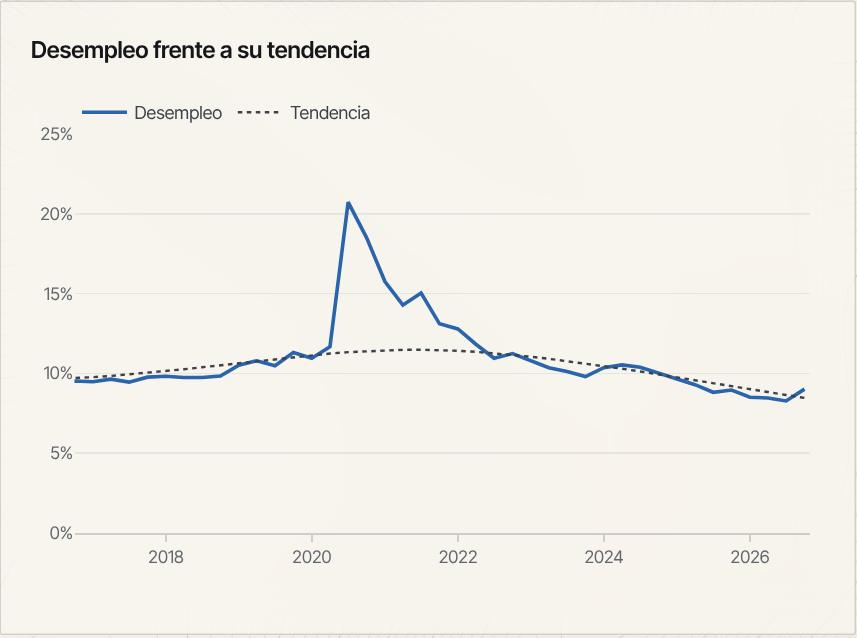
\includegraphics[width=\linewidth,height=0.42\textheight,keepaspectratio]{fig/g-cap-desempleo.jpg}\end{center}
\paragraph{Qué nos cuenta}
Compara la tasa de desempleo con su propia tendencia de largo plazo. La tendencia aproxima el desempleo compatible con una economía en su capacidad; la distancia entre ambas es la «brecha de desempleo», la contraparte laboral de la brecha del producto.

\begin{leer}[Cómo se lee]
Línea azul: tasa de desempleo desestacionalizada (GEIH, DANE), promedio de los tres meses de cada trimestre, en porcentaje. Línea gris punteada: su tendencia estimada con un filtro Hodrick-Prescott de dos colas ($\lambda$ = 1.600). El eje vertical va de 0\% a 25\% y el gráfico arranca en 2010. El salto de 2020 se ve en la línea azul, pero no arrastra la tendencia porque esos trimestres se excluyen e interpolan al estimarla.
\end{leer}

\paragraph{Por qué importa}
Un desempleo por debajo de su tendencia indica un mercado laboral apretado, con más presión sobre salarios y, por esa vía, sobre la inflación de servicios. Por encima, hay trabajadores disponibles y la presión es menor. Es una de las señales que se combinan con la brecha del producto para juzgar cuánta holgura tiene la economía.

\paragraph{Cómo interpretarlo}
\begin{itemize}
\item Azul debajo de la punteada: mercado laboral apretado; azul encima: holgura laboral.
\item La tendencia no es una tasa «natural» oficial: es un suavizado estadístico. Su valor final cambia a medida que llegan datos nuevos, porque el filtro de dos colas usa toda la muestra.
\item Se excluyen 2020T2–2021T2 al estimar la tendencia y se interpolan esos trimestres (la nota del gráfico dice «sin 2020–2021»).
\item La relación con la brecha del producto se mide en el gráfico de la ley de Okun de la página Ciclo.
\end{itemize}
\begin{formulas}[Fórmulas]
\formula{Promedio trimestral}{u\textsubscript{q} = (u\textsubscript{m1} + u\textsubscript{m2} + u\textsubscript{m3}) $\div$ 3}{u = tasa de desempleo desestacionalizada de cada mes del trimestre}
\formula{Brecha de desempleo}{b\textsuperscript{u}\textsubscript{q} = u\textsubscript{q} − u*\textsubscript{q}}{u* = tendencia HP de dos colas ($\lambda$ = 1.600), en puntos porcentuales (pp)}
\end{formulas}
\begin{metodo}[Metodología]
Promedio trimestral de la tasa de desempleo desestacionalizada y su tendencia Hodrick-Prescott ($\lambda$ = 1.600) estimada sin 2020–2021 e interpolada en esos años.
\par\smallskip{\small\textbf{Fuente:} DANE, GEIH desestacionalizada; cálculo propio}
\end{metodo}

\section{¿Dónde está la capacidad? Las regiones}

\subsection{Mapa de las regiones}
\label{g:v-mapa-regiones}
\begin{center}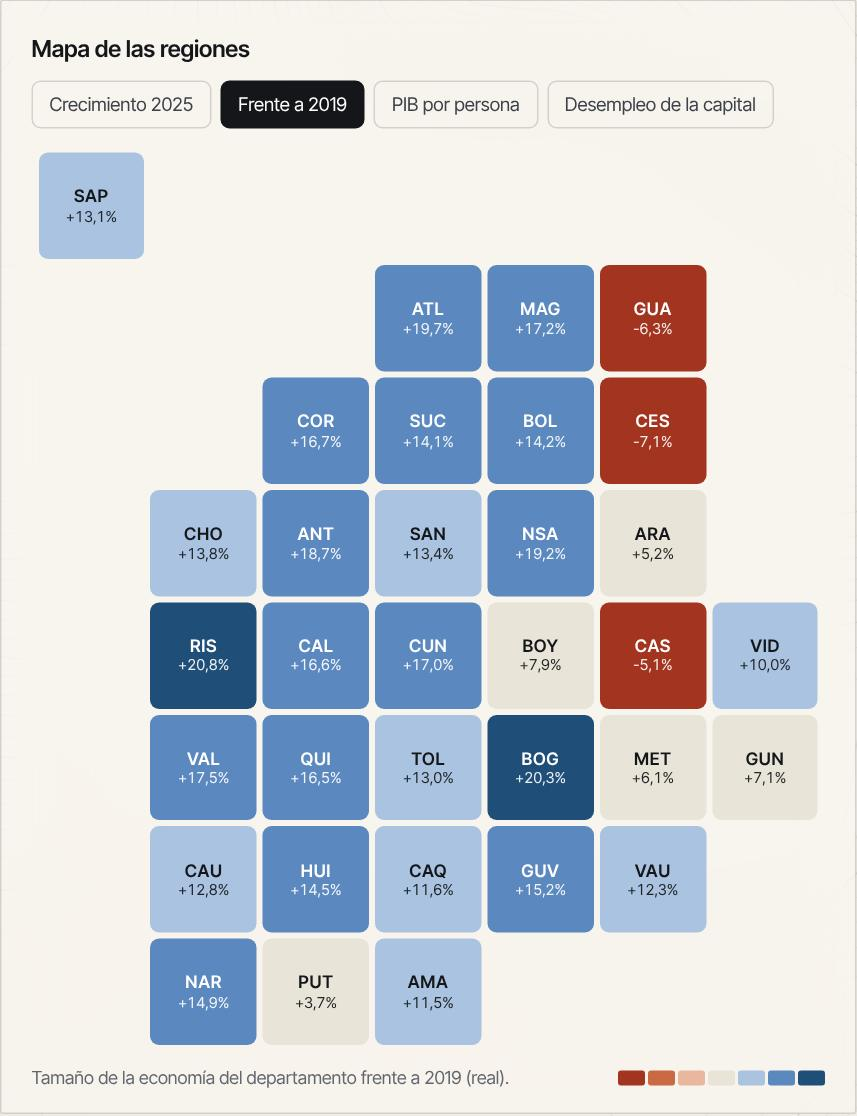
\includegraphics[width=\linewidth,height=0.42\textheight,keepaspectratio]{fig/v-mapa-regiones.jpg}\end{center}
\paragraph{Qué nos cuenta}
Es un mapa esquemático de Colombia en el que cada casilla es un departamento, ubicado aproximadamente en su posición geográfica. Permite ver la geografía de cuatro medidas regionales: el crecimiento del último año, el tamaño de la economía frente a 2019, el PIB por persona y el desempleo de la ciudad capital.

\begin{leer}[Cómo se lee]
Los botones eligen la medida (al abrir, «Frente a 2019»). Cada casilla lleva la abreviatura del departamento y su valor; el color sigue una escala divergente de siete tonos: azul para valores altos, tonos crema para valores intermedios y naranja-terracota para valores bajos. En desempleo la escala se invierte: más desempleo es naranja. Tramos centrales: crecimiento entre −0,25\% y 0,25\%; frente a 2019 entre −1\% y 1\%; PIB por persona entre 85 y 115 (Colombia = 100); desempleo entre 10\% y 12\%. Al pasar el cursor se ven todas las medidas y el sector principal.
\end{leer}

\paragraph{Por qué importa}
Las cifras nacionales esconden grandes diferencias territoriales. El mapa permite identificar de un vistazo regiones dinámicas o rezagadas, de ingreso alto o bajo y con mercados laborales holgados o apretados, información útil para decisiones de localización, distribución comercial o análisis de riesgo regional.

\paragraph{Cómo interpretarlo}
\begin{itemize}
\item Crecimiento: variación real del PIB del departamento frente al año anterior. Frente a 2019: tamaño real de la economía comparado con el año previo a la pandemia.
\item PIB por persona a precios corrientes, con Colombia = 100: 150 significa un ingreso por habitante 50\% mayor al promedio nacional. Departamentos mineros con poca población pueden tener valores altos sin que eso refleje el ingreso de los hogares.
\item Desempleo: tasa de la ciudad capital en año móvil (GEIH, 32 ciudades), no la del departamento; Cundinamarca queda sin dato porque Bogotá se muestra aparte. Las casillas sin dato tienen borde punteado.
\item Mapa no a escala: el área de cada casilla no refleja superficie ni población. El último año de las cuentas departamentales es preliminar.
\end{itemize}
\begin{formulas}[Fórmulas]
\formula{Crecimiento anual}{g\textsubscript{d} = (Y\textsubscript{d,A} $\div$ Y\textsubscript{d,A−1} − 1) $\times$ 100}{Y = PIB real del departamento d; A = último año}
\formula{Frente a 2019}{v\textsubscript{d} = (Y\textsubscript{d,A} $\div$ Y\textsubscript{d,2019} − 1) $\times$ 100}{Y = PIB real (volúmenes encadenados, base 2015)}
\formula{PIB por persona relativo}{I\textsubscript{d} = 100 $\times$ pc\textsubscript{d} $\div$ pc\textsubscript{COL}}{pc = PIB corriente por habitante del departamento y de Colombia}
\end{formulas}

\subsection{Tamaño de cada economía regional frente a 2019}
\label{g:g-cap-regiones}
\begin{center}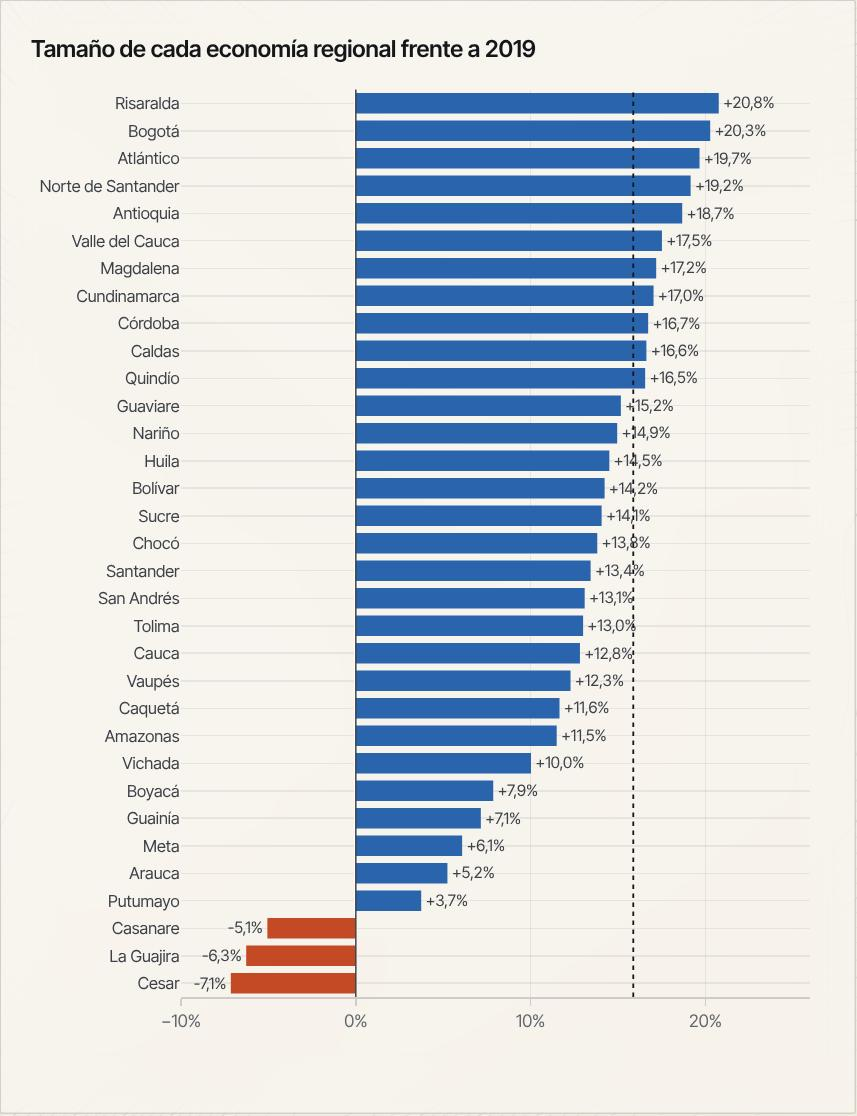
\includegraphics[width=\linewidth,height=0.42\textheight,keepaspectratio]{fig/g-cap-regiones.jpg}\end{center}
\paragraph{Qué nos cuenta}
Compara el tamaño real de la economía de cada uno de los 33 departamentos (incluida Bogotá) en el último año publicado con su tamaño en 2019, el último año antes de la pandemia. Muestra qué regiones ya superaron su nivel previo al choque y cuáles siguen rezagadas.

\begin{leer}[Cómo se lee]
Una barra horizontal por departamento con la variación porcentual del PIB real entre 2019 y el último año disponible; el valor aparece al final de cada barra. Azul: la economía es más grande que en 2019; naranja: más pequeña. La línea vertical continua marca el cero y la punteada el resultado de Colombia en conjunto. Los departamentos van de mayor variación (arriba) a menor (abajo).
\end{leer}

\paragraph{Por qué importa}
La recuperación nacional puede ocultar regiones que no han vuelto a su nivel previo. Las diferencias reflejan la estructura productiva de cada departamento (por ejemplo, la dependencia de la minería) y orientan sobre dónde está el dinamismo de la demanda, el empleo y la base de clientes regional.

\paragraph{Cómo interpretarlo}
\begin{itemize}
\item Barras a la derecha de la línea punteada: el departamento creció más que el país desde 2019; a la izquierda, menos.
\item Una variación negativa indica que la economía departamental aún produce menos, en términos reales, que antes de la pandemia.
\item Las cuentas departamentales se publican con rezago anual y el último año es preliminar: puede revisarse en la siguiente publicación.
\item Para ver de qué vive cada región y qué tan concentrada está, compare con los gráficos de estructura productiva y diversificación.
\end{itemize}
\begin{formulas}[Fórmulas]
\formula{Variación frente a 2019}{v\textsubscript{d} = (Y\textsubscript{d,A} $\div$ Y\textsubscript{d,2019} − 1) $\times$ 100}{Y = PIB real del departamento d (volúmenes encadenados, base 2015); A = último año publicado}
\end{formulas}
\begin{metodo}[Metodología]
PIB real de cada departamento en el último año publicado frente a 2019 (volúmenes encadenados, base 2015). Último año preliminar.
\par\smallskip{\small\textbf{Fuente:} DANE, Cuentas nacionales departamentales, base 2015 (anexos de PIB por departamento y por actividad)}
\end{metodo}

\section{¿De qué vive cada región?}

\subsection{Estructura productiva por departamento (2025)}
\label{g:g-cap-estructura}
\begin{center}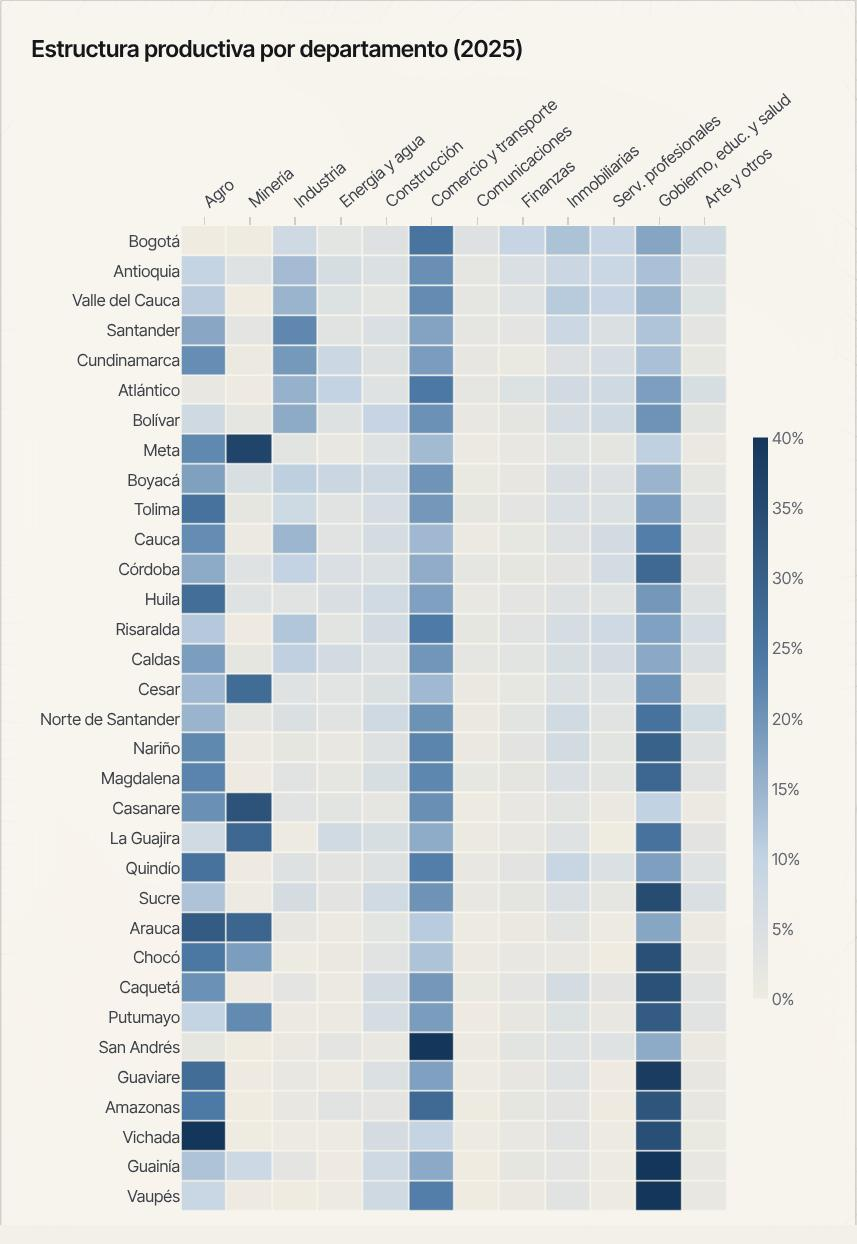
\includegraphics[width=\linewidth,height=0.42\textheight,keepaspectratio]{fig/g-cap-estructura.jpg}\end{center}
\paragraph{Qué nos cuenta}
Muestra de qué vive cada departamento: el peso de cada una de las 12 grandes ramas de actividad en su valor agregado. Revela regiones dominadas por un solo sector (minería, agro, Gobierno) frente a economías más mezcladas de industria y servicios.

\begin{leer}[Cómo se lee]
Mapa de calor: cada fila es un departamento y cada columna una rama (agro, minería, industria, energía y agua, construcción, comercio y transporte, comunicaciones, finanzas, inmobiliarias, servicios profesionales, Gobierno-educación-salud, arte y otros). El color es la participación en porcentaje, de blanco (0\%) a azul oscuro; la escala se satura en 40\%, así que pesos mayores se ven con el tono más oscuro. Los departamentos van ordenados por tamaño de su PIB, del más grande arriba al más pequeño abajo. Cada fila suma 100\%.
\end{leer}

\paragraph{Por qué importa}
La composición sectorial determina cómo responde cada región a los choques: precios del petróleo y del carbón, clima, gasto público o crédito. Para un inversionista, indica la sensibilidad regional a ciclos de materias primas y la profundidad de los mercados de servicios en cada territorio.

\paragraph{Cómo interpretarlo}
\begin{itemize}
\item Una celda muy oscura aislada en una fila señala dependencia de un sector; filas con tonos medios repartidos indican una economía diversificada.
\item Se usan precios corrientes del último año: un salto en el precio de un producto (por ejemplo, el petróleo) puede aumentar la participación de la minería sin que cambie el volumen producido.
\item Las participaciones se calculan sobre el valor agregado sin impuestos, por lo que difieren levemente de las del PIB.
\item El gráfico de diversificación contiguo resume cada fila en un solo número.
\end{itemize}
\begin{formulas}[Fórmulas]
\formula{Participación sectorial}{s\textsubscript{i,d} = VA\textsubscript{i,d} $\div$ $\Sigma$\textsubscript{j} VA\textsubscript{j,d} $\times$ 100}{VA = valor agregado a precios corrientes de la rama i en el departamento d; suma sobre las 12 ramas (sin impuestos)}
\end{formulas}
\begin{metodo}[Metodología]
Participación de cada una de las 12 agrupaciones CIIU en el valor agregado del departamento (sin impuestos), a precios corrientes del último año.
\par\smallskip{\small\textbf{Fuente:} DANE, Cuentas nacionales departamentales, base 2015 (anexos de PIB por departamento y por actividad)}
\end{metodo}

\subsection{Diversificación: número equivalente de sectores}
\label{g:g-cap-diversificacion}
\begin{center}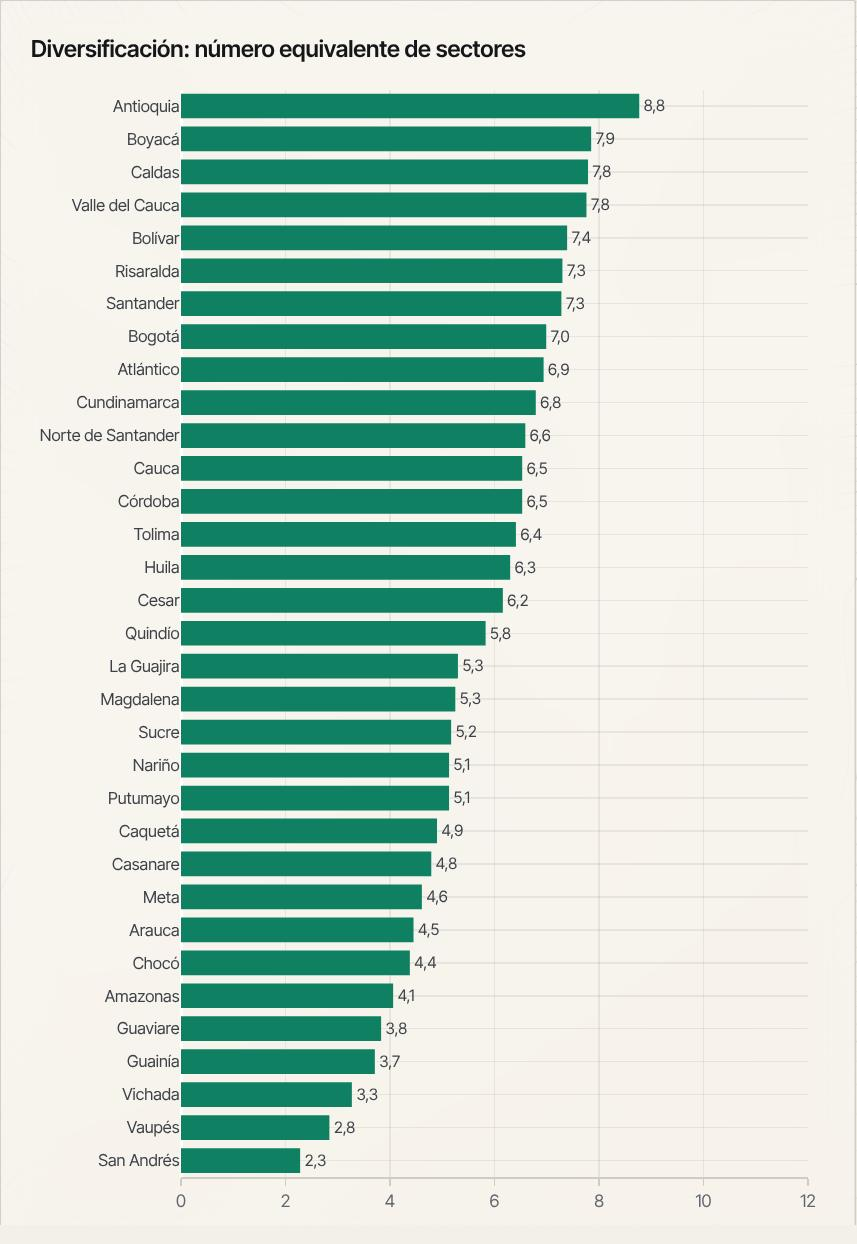
\includegraphics[width=\linewidth,height=0.42\textheight,keepaspectratio]{fig/g-cap-diversificacion.jpg}\end{center}
\paragraph{Qué nos cuenta}
Resume en un número qué tan diversificada es la economía de cada departamento: el «número equivalente de sectores», es decir, cuántos sectores del mismo tamaño producirían la misma concentración observada. Es el inverso del índice de Herfindahl-Hirschman, una medida estándar de concentración.

\begin{leer}[Cómo se lee]
Una barra horizontal por departamento, con el valor escrito al final. El eje va de 0 a 12: 12 sería el máximo teórico (las 12 ramas con el mismo peso) y 1 una economía que depende de un único sector. Los departamentos están ordenados del más diversificado (arriba) al más concentrado (abajo). Se calcula con las participaciones del gráfico de estructura productiva.
\end{leer}

\paragraph{Por qué importa}
Las regiones concentradas son más vulnerables cuando su sector principal se frena, por ejemplo ante una caída de precios de materias primas o un cambio regulatorio. Las diversificadas suelen tener ciclos más estables. Para evaluar riesgos regionales, este número complementa al crecimiento y al tamaño de cada economía.

\paragraph{Cómo interpretarlo}
\begin{itemize}
\item Un valor alto (cerca de 8 o más) indica una economía repartida entre muchas ramas; un valor bajo (cerca de 2 o 3), una fuerte dependencia de una o dos.
\item El índice no dice cuál es el sector dominante: para eso, vea la fila del departamento en el mapa de estructura productiva.
\item Como usa precios corrientes, puede moverse con los precios relativos (por ejemplo, del petróleo) aunque la estructura física no cambie.
\item La desagregación en 12 ramas limita el valor máximo y oculta la diversificación dentro de cada rama.
\end{itemize}
\begin{formulas}[Fórmulas]
\formula{Índice de Herfindahl-Hirschman}{HHI\textsubscript{d} = $\Sigma$\textsubscript{i} s\textsubscript{i,d}\textsuperscript{2}}{s = participación (en tanto por uno) de la rama i en el valor agregado del departamento d}
\formula{Número equivalente de sectores}{N\textsubscript{d} = 1 $\div$ HHI\textsubscript{d}}{va de 1 (un solo sector) a 12 (12 ramas iguales)}
\end{formulas}
\begin{metodo}[Metodología]
Número equivalente = 1 / $\Sigma$ s\textsubscript{i}\textsuperscript{2}, donde s\textsubscript{i} es la participación de la rama i en el valor agregado del departamento (Herfindahl, 1950; Hirschman, 1964).
\par\smallskip{\small\textbf{Fuente:} DANE, Cuentas nacionales departamentales, base 2015 (anexos de PIB por departamento y por actividad)}
\end{metodo}

\section*{Lecturas de la página}
\begin{itemize}\small
\item \textbf{Okun, A. M. (1962). Potential GNP: Its Measurement and Significance. Proceedings of the Business and Economic Statistics Section, ASA.} Producto potencial y relación entre holgura del producto y del empleo.
\item \textbf{OIT (2013). Resolución sobre las estadísticas del trabajo, la ocupación y la subutilización de la fuerza de trabajo. 19.ª CIET.} Definición de subocupación, fuerza de trabajo potencial y medida compuesta de subutilización.
\item \textbf{Hodrick, R. J. y Prescott, E. C. (1997). Postwar U.S. Business Cycles. Journal of Money, Credit and Banking, 29(1), 1–16.} Tendencia de cada sector y del desempleo.
\item \textbf{Hirschman, A. O. (1964). The Paternity of an Index. American Economic Review, 54(5), 761; Herfindahl, O. C. (1950). Concentration in the Steel Industry. Columbia University.} Índice de concentración y número equivalente de sectores.
\item \textbf{DANE. Cuentas nacionales departamentales, base 2015: metodología (CD-01).} PIB y valor agregado por departamento y actividad.
\end{itemize}

\chapter{Empleo}
\label{atlas:empleo}

{\large\sffamily\bfseries Empleo e informalidad\par}\medskip

Cuántos trabajan, dónde y cómo: desempleo, informalidad, empleo por sector y por tipo de contrato, brechas entre mujeres y hombres, jóvenes, campo y ciudad, y las 32 capitales.

{\small\color{cmmuted}Página del sitio: \url{https://stv-quant.github.io/ColombiaMacro-USBCali/empleo/}}

\section{¿Cómo está el empleo y cuánto es informal?}

\subsection{Tasa de desempleo}
\label{g:g-desempleo}
\begin{center}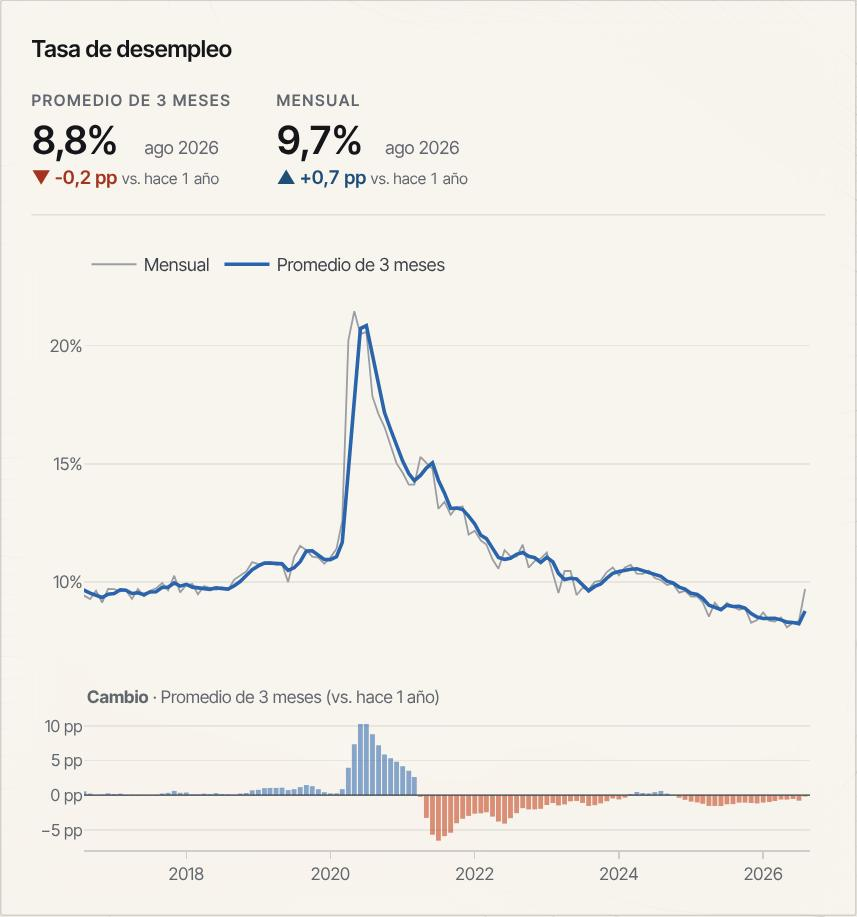
\includegraphics[width=\linewidth,height=0.42\textheight,keepaspectratio]{fig/g-desempleo.jpg}\end{center}
\paragraph{Qué nos cuenta}
Muestra la tasa de desempleo nacional: la proporción de la fuerza de trabajo (personas que trabajan o buscan trabajo) que busca empleo y no lo consigue. Es la serie desestacionalizada que publica el DANE a partir de la Gran Encuesta Integrada de Hogares (GEIH), la encuesta mensual con la que se mide el mercado laboral. Resume en un número la holgura del mercado de trabajo y su evolución a lo largo del ciclo económico.

\begin{leer}[Cómo se lee]
Panel superior, en porcentaje: la línea gris delgada es el dato mensual desestacionalizado y la línea azul gruesa es su promedio móvil de 3 meses, que filtra el ruido de muestreo de la encuesta. Panel inferior: barras con el cambio del promedio de 3 meses frente al mismo mes un año antes, en puntos porcentuales (pp); azules cuando el desempleo sube y naranjas cuando baja. La vista inicial abarca los últimos diez años; el recuadro flotante muestra ambos paneles a la vez.
\end{leer}

\paragraph{Por qué importa}
El desempleo es el termómetro más directo del bienestar de los hogares y de la presión sobre salarios e ingresos. Un mercado laboral holgado limita el consumo y las presiones de costos; uno estrecho los impulsa. Por eso el Banco de la República lo sigue para calibrar la tasa de interés, y los inversionistas lo usan para leer la demanda interna, la calidad de la cartera de los bancos y el entorno social y fiscal.

\paragraph{Cómo interpretarlo}
\begin{itemize}
\item Barras naranjas persistentes indican que el desempleo está por debajo del de un año antes; barras azules seguidas, que el mercado laboral se debilita.
\item Conviene mirar la línea azul y no el dato mensual aislado: movimientos de 0,3–0,5 pp en un solo mes pueden ser ruido de la encuesta.
\item El salto de 2020 (pandemia) es el episodio extremo de la serie y distorsiona los cambios anuales del año siguiente (efecto base).
\item La tasa puede bajar porque se crean empleos o porque menos personas buscan trabajo; contrástela con la participación laboral (gráfico de mujeres y hombres) y con los empleos por rama.
\item El DANE revisa la desestacionalización cuando llegan datos nuevos, por lo que los últimos meses pueden cambiar levemente.
\end{itemize}
\begin{formulas}[Fórmulas]
\formula{Tasa de desempleo}{TD\textsubscript{t} = D\textsubscript{t} $\div$ FT\textsubscript{t} $\times$ 100}{D = desocupados; FT = fuerza de trabajo (ocupados + desocupados); serie desestacionalizada del DANE}
\formula{Promedio de 3 meses}{TD3\textsubscript{t} = (TD\textsubscript{t} + TD\textsubscript{t−1} + TD\textsubscript{t−2}) $\div$ 3}{t = mes}
\formula{Cambio anual (panel inferior)}{$\Delta$TD3\textsubscript{t} = TD3\textsubscript{t} − TD3\textsubscript{t−12}}{en puntos porcentuales}
\end{formulas}
\begin{metodo}[Metodología]
Tasa de desempleo = desocupados / fuerza de trabajo, serie desestacionalizada del DANE; la línea azul promedia 3 meses. Panel inferior: cambio frente a un año antes, en puntos.
\par\smallskip{\small\textbf{Fuente:} DANE, Gran Encuesta Integrada de Hogares (GEIH)}
\end{metodo}

\subsection{Proporción de ocupados informales}
\label{g:g-informal}
\begin{center}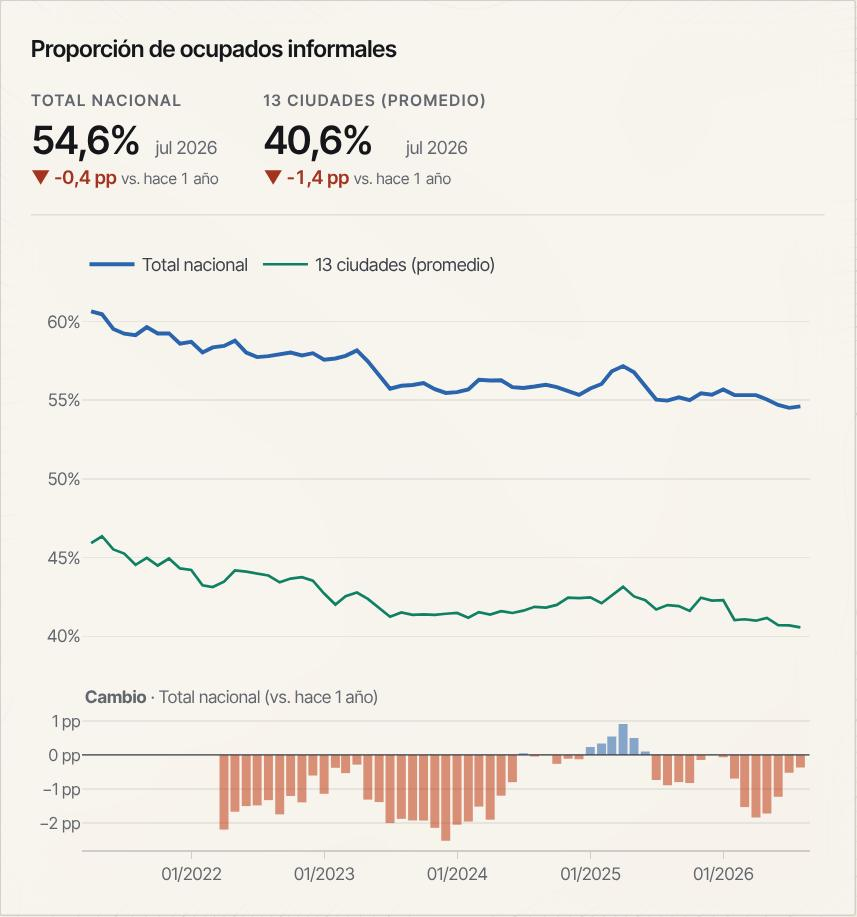
\includegraphics[width=\linewidth,height=0.42\textheight,keepaspectratio]{fig/g-informal.jpg}\end{center}
\paragraph{Qué nos cuenta}
Muestra qué porcentaje de las personas ocupadas trabaja en la informalidad según la definición vigente del DANE, alineada con la Organización Internacional del Trabajo (OIT): ocupados sin afiliación a la seguridad social o que trabajan en unidades económicas no registradas. Compara el total nacional con el agregado de las 13 ciudades principales y sus áreas metropolitanas, donde la informalidad es menor que en el resto del país.

\begin{leer}[Cómo se lee]
Panel superior, en porcentaje de los ocupados: línea azul = total nacional; línea verde = 13 ciudades y áreas metropolitanas. Cada punto es un trimestre móvil (tres meses que terminan en el mes indicado). Panel inferior: cambio de la tasa nacional frente al mismo trimestre móvil de un año antes, en pp; barras naranjas cuando la informalidad baja y azules cuando sube. La serie comienza en 2021 con la nueva definición.
\end{leer}

\paragraph{Por qué importa}
La informalidad es uno de los rasgos estructurales del mercado laboral colombiano: limita la base tributaria y de cotizantes a pensiones y salud, reduce la productividad y deja a los hogares con ingresos más volátiles. Para un inversionista indica la calidad del empleo detrás de las cifras de desempleo, la profundidad del mercado de consumo formal y el margen fiscal del Estado.

\paragraph{Cómo interpretarlo}
\begin{itemize}
\item Una caída sostenida (barras naranjas) significa que una mayor parte de los ocupados cotiza a la seguridad social o trabaja en empresas registradas.
\item La brecha entre el total nacional y las 13 ciudades refleja el peso del campo y de las ciudades intermedias, donde predominan el trabajo por cuenta propia y el agro.
\item Cambios menores a 1 pp en un año pueden estar dentro del error de muestreo de la encuesta.
\item No es comparable con las cifras anteriores a 2021 (otra definición y otro marco muestral); compárela con la composición del empleo por posición ocupacional y con la informalidad por sector.
\end{itemize}
\begin{formulas}[Fórmulas]
\formula{Proporción de informalidad}{INF\textsubscript{t} = I\textsubscript{t} $\div$ O\textsubscript{t} $\times$ 100}{I = ocupados informales; O = ocupados; trimestre móvil que termina en el mes t}
\formula{Cambio anual (panel inferior)}{$\Delta$INF\textsubscript{t} = INF\textsubscript{t} − INF\textsubscript{t−12}}{en puntos porcentuales}
\end{formulas}
\begin{metodo}[Metodología]
Proporción de ocupados informales (definición DANE 2023, alineada con la OIT): sin seguridad social o en unidades no registradas. Trimestres móviles desde 2021; no comparable con la serie anterior.
\par\smallskip{\small\textbf{Fuente:} DANE, GEIH – empleo informal y seguridad social}
\end{metodo}

\subsection{Informalidad por sector (may–jul 2026)}
\label{g:g-inf-ramas}
\begin{center}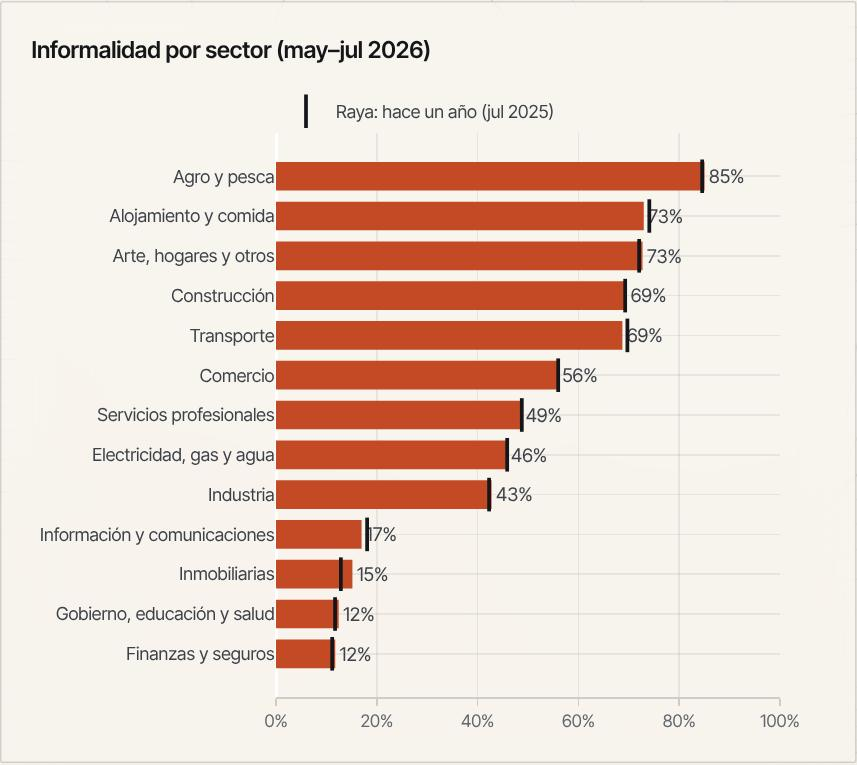
\includegraphics[width=\linewidth,height=0.42\textheight,keepaspectratio]{fig/g-inf-ramas.jpg}\end{center}
\paragraph{Qué nos cuenta}
Compara la informalidad entre las 13 ramas de actividad en que la GEIH agrupa el empleo, para el último trimestre móvil disponible. Muestra que la informalidad no es pareja: es casi generalizada en el agro, el comercio, el alojamiento y comida o el transporte, y baja en finanzas, en el sector público, la educación y la salud o en los servicios públicos. Permite ver dónde se concentra el problema y si mejora o empeora en cada sector.

\begin{leer}[Cómo se lee]
Eje horizontal de 0\% a 100\%: proporción de los ocupados de cada rama que son informales, total nacional. Las barras naranjas son el dato del último trimestre móvil, ordenadas de menor a mayor; la raya vertical negra sobre cada barra es el dato del mismo trimestre móvil un año antes. El recuadro flotante muestra la tasa, su cambio en pp frente a un año antes y cuántos informales y ocupados hay en la rama, en millones de personas.
\end{leer}

\paragraph{Por qué importa}
La informalidad sectorial explica por qué el crecimiento de ciertas ramas genera más o menos empleo formal, cotizaciones y recaudo. Para un inversionista ayuda a dimensionar los costos laborales, la exposición regulatoria y el tamaño del mercado formal en cada actividad, y a entender qué sectores pesan en el promedio nacional.

\paragraph{Cómo interpretarlo}
\begin{itemize}
\item Una barra a la izquierda de su raya indica que la informalidad del sector bajó frente a un año antes; a la derecha, que subió.
\item Una rama con tasa alta pero pocos ocupados pesa poco en el total; mire el número de personas en el recuadro flotante.
\item El promedio nacional también cambia si el empleo se desplaza entre sectores, aunque la tasa de cada uno no varíe (efecto composición).
\item Las ramas pequeñas tienen más error de muestreo; diferencias de 1–2 pp en un año pueden no ser significativas.
\end{itemize}
\begin{formulas}[Fórmulas]
\formula{Informalidad por rama}{INF\textsubscript{r} = I\textsubscript{r} $\div$ O\textsubscript{r} $\times$ 100}{I = informales; O = ocupados de la rama r; trimestre móvil, total nacional}
\formula{Cambio frente a un año antes}{$\Delta$INF\textsubscript{r} = INF\textsubscript{r,t} − INF\textsubscript{r,t−12}}{en pp (recuadro flotante)}
\end{formulas}
\begin{metodo}[Metodología]
Informales / ocupados de cada rama, total nacional. La raya vertical es el dato de un año antes.
\par\smallskip{\small\textbf{Fuente:} DANE, GEIH – empleo informal y seguridad social}
\end{metodo}

\subsection{Informalidad por ciudad (may–jul 2026)}
\label{g:g-informal-ciudades}
\begin{center}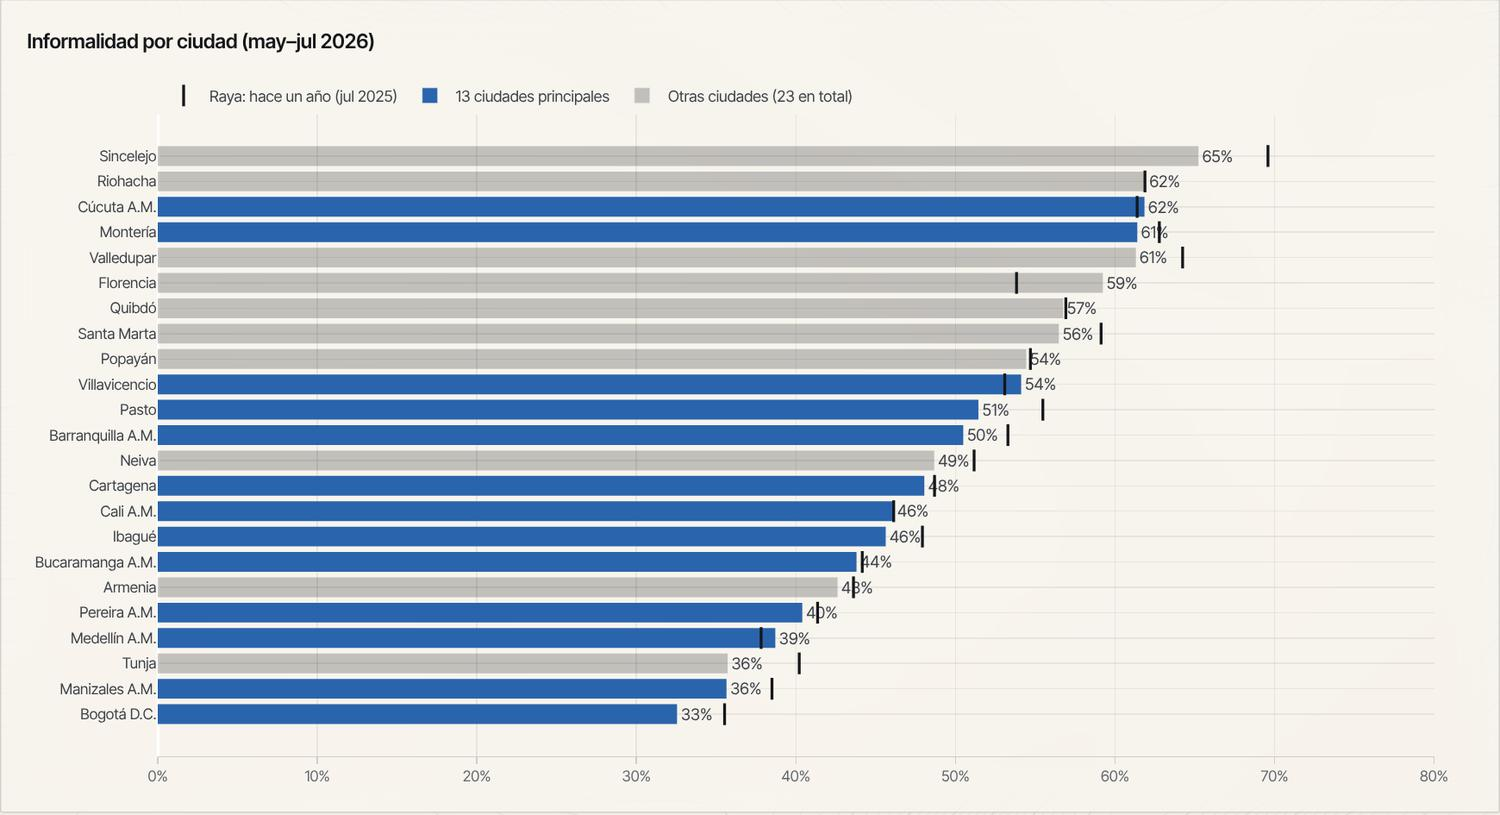
\includegraphics[width=\linewidth,height=0.42\textheight,keepaspectratio]{fig/g-informal-ciudades.jpg}\end{center}
\paragraph{Qué nos cuenta}
Ordena las 23 ciudades y áreas metropolitanas (A.M.) que mide la GEIH según la proporción de sus ocupados que trabajan en la informalidad. Muestra que el problema tiene una geografía marcada: las ciudades más grandes e industriales tienden a tener menos informalidad que las ciudades intermedias y de la región Caribe, y permite ver si cada ciudad mejora o empeora frente a un año antes.

\begin{leer}[Cómo se lee]
Cada barra horizontal es una ciudad, ordenada de menor a mayor informalidad; el eje va de 0\% a 80\% de los ocupados. Las barras azules son las 13 ciudades y áreas metropolitanas principales; las grises, las otras 10 capitales. La raya vertical negra sobre cada barra marca el dato del mismo trimestre móvil un año antes. Al pasar el cursor se ven la tasa, el dato de hace un año y el cambio en pp.
\end{leer}

\paragraph{Por qué importa}
La informalidad local indica qué tan formal es el mercado laboral en cada plaza: afecta la capacidad de los hogares de acceder a crédito, la base de cotización a la seguridad social y el recaudo de impuestos locales. Para un inversionista ayuda a dimensionar el mercado formal de consumo y la disponibilidad de trabajadores formales en cada ciudad.

\paragraph{Cómo interpretarlo}
\begin{itemize}
\item Una barra que termina a la izquierda de su raya indica que la informalidad de esa ciudad bajó frente a un año antes; a la derecha, que subió.
\item Las diferencias entre ciudades reflejan su estructura productiva (industria y servicios modernos frente a comercio y servicios personales) más que cambios de corto plazo.
\item Las ciudades pequeñas tienen muestras más pequeñas en la GEIH: cambios de 1–2 pp en un año pueden estar dentro del error de muestreo.
\item Compárelo con la informalidad por rama: una ciudad con mucho comercio y transporte tiende a tener tasas más altas.
\end{itemize}
\begin{formulas}[Fórmulas]
\formula{Informalidad de la ciudad}{INF\textsubscript{c} = I\textsubscript{c} $\div$ O\textsubscript{c} $\times$ 100}{I = ocupados informales; O = ocupados de la ciudad c; trimestre móvil}
\formula{Cambio en un año}{$\Delta$INF\textsubscript{c} = INF\textsubscript{c,t} − INF\textsubscript{c,t−12}}{en puntos porcentuales (pp)}
\end{formulas}
\begin{metodo}[Metodología]
Proporción de ocupados informales en cada una de las 23 ciudades y áreas metropolitanas (A.M.); en azul las 13 principales. La raya es el dato de un año antes.
\par\smallskip{\small\textbf{Fuente:} DANE, GEIH – empleo informal y seguridad social}
\end{metodo}

\section{¿Dónde se crean (y se pierden) los empleos?}

\subsection{Empleos creados o perdidos en un año, por rama (miles)}
\label{g:g-emp-ramas}
\begin{center}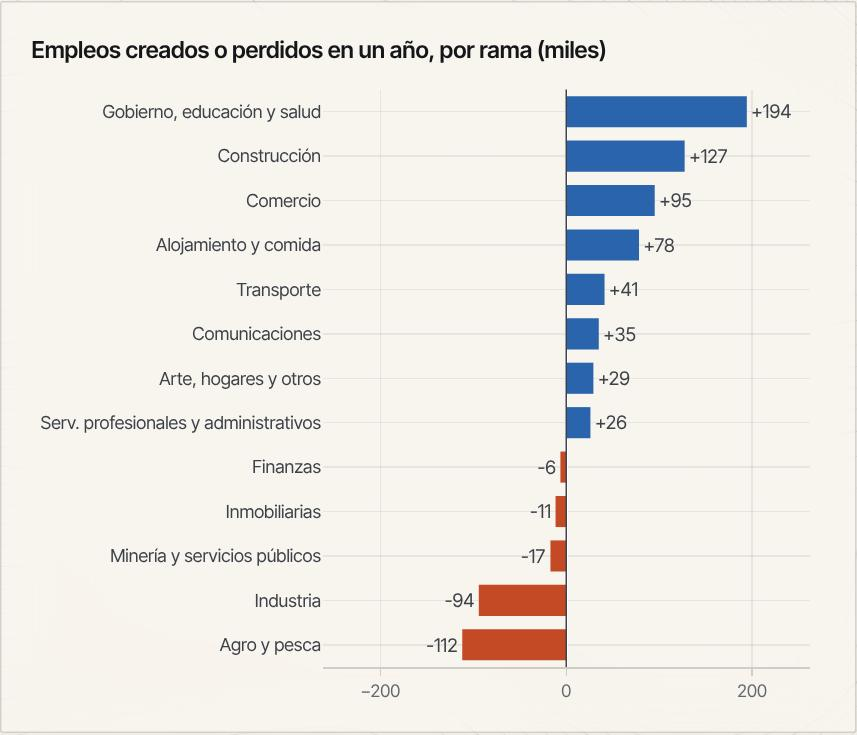
\includegraphics[width=\linewidth,height=0.42\textheight,keepaspectratio]{fig/g-emp-ramas.jpg}\end{center}
\paragraph{Qué nos cuenta}
Muestra cuántos empleos ganó o perdió cada rama de actividad en el último año, en miles de personas. Responde a la pregunta de dónde se está creando el empleo: qué sectores explican el aumento (o la caída) del número total de ocupados. Usa las 13 agrupaciones de ramas de la GEIH (clasificación CIIU Rev. 4 adaptada para Colombia).

\begin{leer}[Cómo se lee]
Cada barra horizontal es una rama, ordenada del mayor aumento (arriba) a la mayor caída (abajo). El eje está en miles de personas y la línea vertical marca el cero. Barras azules: la rama tiene más ocupados que un año antes; naranjas: tiene menos. La cifra junto a cada barra es el cambio redondeado. Se compara el promedio de los últimos 3 meses con el de los mismos 3 meses del año anterior, en datos sin desestacionalizar.
\end{leer}

\paragraph{Por qué importa}
El empleo sectorial conecta el crecimiento del PIB con los hogares: un sector puede crecer en producción sin contratar, o contratar mucho con poca producción. Para un inversionista indica qué actividades sostienen el ingreso laboral y el consumo, y cuáles están ajustando su planta de personal, una señal temprana sobre su demanda y sus márgenes.

\paragraph{Cómo interpretarlo}
\begin{itemize}
\item La suma de las barras aproxima el cambio anual del total de ocupados; si unas pocas ramas explican casi todo el aumento, el empleo depende de pocos motores.
\item Comparar los mismos meses del año anterior evita la estacionalidad (cosechas, temporada de fin de año) sin modelos estadísticos.
\item Cambios de pocas decenas de miles en ramas pequeñas pueden estar dentro del error de muestreo de la encuesta.
\item La GEIH agrupa la minería con los servicios públicos (electricidad, gas y agua); compárelo con el crecimiento del PIB por sectores y con la informalidad por rama.
\end{itemize}
\begin{formulas}[Fórmulas]
\formula{Promedio de 3 meses}{Ō\textsubscript{r,t} = (O\textsubscript{r,t} + O\textsubscript{r,t−1} + O\textsubscript{r,t−2}) $\div$ 3}{O = ocupados de la rama r en el mes t (miles)}
\formula{Empleos creados o perdidos}{$\Delta$O\textsubscript{r} = Ō\textsubscript{r,t} − Ō\textsubscript{r,t−12}}{en miles de personas}
\end{formulas}
\begin{metodo}[Metodología]
Población ocupada por rama de actividad (CIIU Rev. 4 A.C., 13 agrupaciones de la GEIH), total nacional, sin desestacionalizar: promedio de los últimos 3 meses menos el promedio de los mismos 3 meses del año anterior. La GEIH agrupa la minería con los servicios públicos.
\par\smallskip{\small\textbf{Fuente:} DANE, Gran Encuesta Integrada de Hogares (GEIH), anexo mensual}
\end{metodo}

\subsection{Empleo por rama frente a 2019}
\label{g:g-emp-ramas-2019}
\begin{center}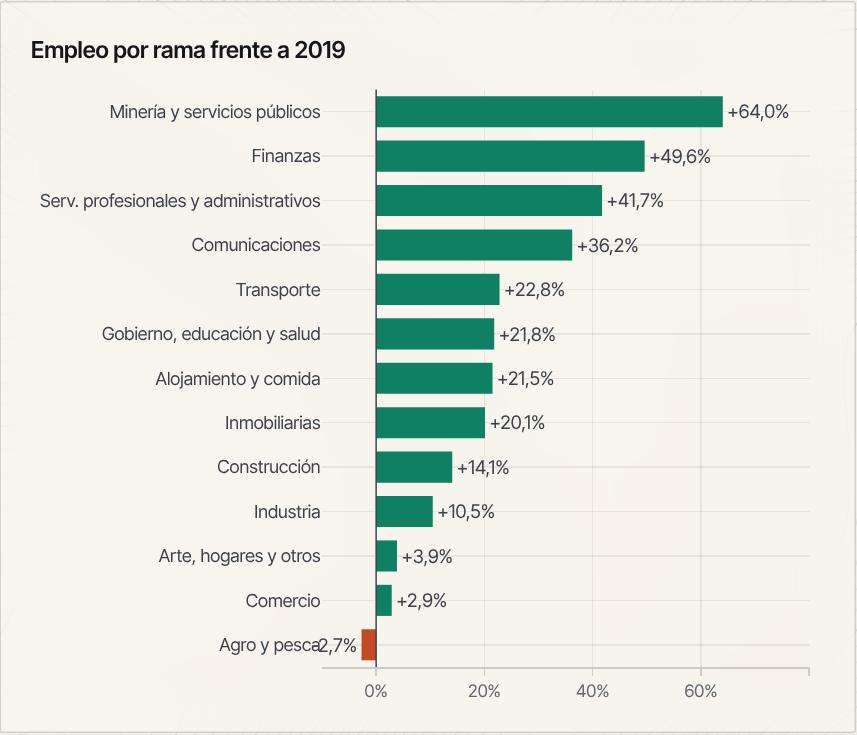
\includegraphics[width=\linewidth,height=0.42\textheight,keepaspectratio]{fig/g-emp-ramas-2019.jpg}\end{center}
\paragraph{Qué nos cuenta}
Compara el empleo actual de cada rama con el de 2019, el último año completo antes de la pandemia. Muestra qué sectores ya superan su nivel de empleo prepandemia y cuáles siguen por debajo, es decir, cómo cambió la estructura del empleo después del choque de 2020. Es una mirada de mediano plazo que complementa el cambio de un año.

\begin{leer}[Cómo se lee]
Cada barra horizontal es una rama de la GEIH, ordenada de mayor a menor variación. El eje muestra la variación porcentual del promedio de ocupados de los últimos 12 meses frente al promedio de los 12 meses de 2019. Barras verdes: la rama emplea más personas que en 2019; naranjas: menos. La línea vertical marca el 0\% (mismo nivel que en 2019).
\end{leer}

\paragraph{Por qué importa}
Revela cambios estructurales que el dato de un año no muestra: sectores que crecieron de forma sostenida y otros que perdieron peso de manera duradera. Para un inversionista ayuda a separar recuperaciones cíclicas de transformaciones de largo plazo en la demanda de trabajo, la productividad y los hábitos de consumo.

\paragraph{Cómo interpretarlo}
\begin{itemize}
\item Una barra verde amplia indica un sector cuyo empleo creció por encima del nivel prepandemia; una naranja, que no ha recuperado los puestos de 2019 o que se encoge por razones estructurales (automatización, cambio de demanda).
\item Promediar 12 meses elimina la estacionalidad y reduce el ruido de la encuesta.
\item Una caída del empleo no implica una caída de la producción: puede reflejar ganancias de productividad; compárelo con el PIB por sectores.
\item La comparación depende del año base: si 2019 fue un año atípico para una rama, la variación lo arrastra.
\end{itemize}
\begin{formulas}[Fórmulas]
\formula{Variación frente a 2019}{V\textsubscript{r} = (Ō\textsuperscript{12}\textsubscript{r,t} $\div$ Ō\textsubscript{r,2019} − 1) $\times$ 100}{Ō\textsuperscript{12} = promedio de ocupados de los últimos 12 meses; Ō\textsubscript{2019} = promedio de los 12 meses de 2019; r = rama}
\end{formulas}
\begin{metodo}[Metodología]
Promedio de los últimos 12 meses frente al promedio de 2019.
\par\smallskip{\small\textbf{Fuente:} DANE, Gran Encuesta Integrada de Hogares (GEIH), anexo mensual}
\end{metodo}

\section{¿Qué tipo de empleo se crea?}

\subsection{¿Cómo trabajan los colombianos? Composición del empleo}
\label{g:g-emp-posicion}
\begin{center}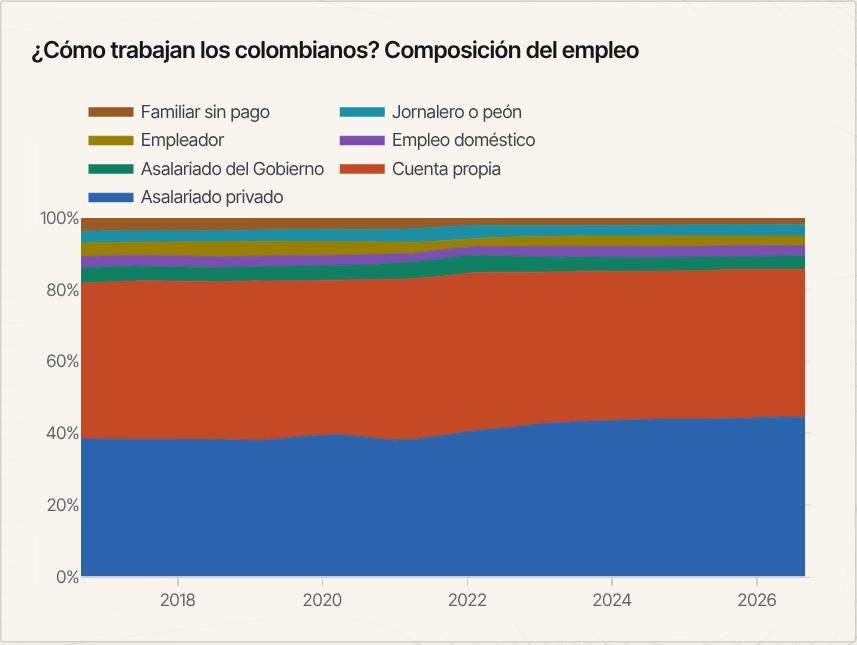
\includegraphics[width=\linewidth,height=0.42\textheight,keepaspectratio]{fig/g-emp-posicion.jpg}\end{center}
\paragraph{Qué nos cuenta}
Muestra cómo se reparte el empleo según la posición ocupacional, es decir, la relación de cada persona con su trabajo según la clasificación internacional CISE-93 de la OIT: asalariados del sector privado, trabajadores por cuenta propia, empleados del Gobierno, empleo doméstico, empleadores, jornaleros y familiares sin pago. Revela la calidad del empleo: cuánto descansa en contratos asalariados y cuánto en el trabajo independiente.

\begin{leer}[Cómo se lee]
Áreas apiladas que suman el 100\% de los ocupados (eje de 0\% a 100\%), desde 2011. De abajo hacia arriba: azul = asalariado privado; naranja = cuenta propia; verde = asalariado del Gobierno; morado = empleo doméstico; ámbar = empleador; azul verdoso = jornalero o peón; café = familiar sin pago. Cada participación usa promedios móviles de 12 meses de los ocupados, lo que elimina la estacionalidad. Se omite la categoría «otro» (menos de 0,1\%).
\end{leer}

\paragraph{Por qué importa}
En Colombia cerca de la mitad de los ocupados trabaja por cuenta propia o en posiciones sin contrato, lo que se asocia con informalidad, ingresos inestables y baja productividad. Un aumento del peso de los asalariados suele acompañar la formalización y la expansión de las empresas. Para un inversionista es una señal de la profundidad del mercado laboral formal, la estabilidad del ingreso de los hogares y la base de cotizantes.

\paragraph{Cómo interpretarlo}
\begin{itemize}
\item Si la franja azul se ensancha a costa de la naranja, el empleo se está volviendo más asalariado; lo contrario indica más trabajo independiente.
\item Los asalariados privados son en su mayoría formales, pero no todos; para la informalidad exacta use el gráfico de informalidad.
\item En las recesiones el trabajo por cuenta propia tiende a absorber a quienes pierden un empleo asalariado; obsérvelo alrededor de 2020.
\item Por ser un promedio de 12 meses, los cambios aparecen de forma gradual y con rezago; el gráfico de cambio en un año por posición muestra el movimiento reciente.
\end{itemize}
\begin{formulas}[Fórmulas]
\formula{Promedio de 12 meses}{Ō\textsubscript{p,t} = (1 $\div$ 12) $\times$ $\Sigma$\textsubscript{k=0..11} O\textsubscript{p,t−k}}{O = ocupados en la posición p en el mes t}
\formula{Participación}{S\textsubscript{p,t} = Ō\textsubscript{p,t} $\div$ $\Sigma$\textsubscript{j} Ō\textsubscript{j,t} $\times$ 100}{j recorre las siete posiciones graficadas}
\end{formulas}
\begin{metodo}[Metodología]
Posición ocupacional según la CISE-93 (OIT): participación de cada categoría en los ocupados, con promedios móviles de 12 meses. Se omite la categoría «otro» (menos de 0,1\%).
\par\smallskip{\small\textbf{Fuente:} DANE, Gran Encuesta Integrada de Hogares (GEIH), anexo mensual}
\end{metodo}

\subsection{Cambio en un año por posición ocupacional (miles)}
\label{g:g-emp-posicion-cambio}
\begin{center}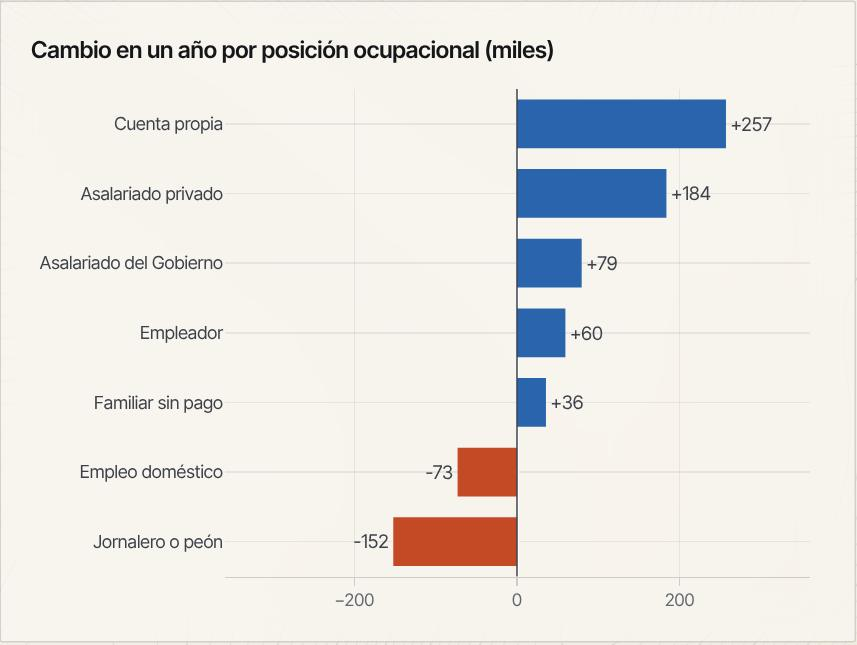
\includegraphics[width=\linewidth,height=0.42\textheight,keepaspectratio]{fig/g-emp-posicion-cambio.jpg}\end{center}
\paragraph{Qué nos cuenta}
Muestra cuántos ocupados ganó o perdió cada posición ocupacional (CISE-93 de la OIT) en el último año, en miles de personas. Indica qué tipo de empleo se está creando: si el aumento del número de ocupados viene de puestos asalariados, en su mayoría con contrato, o del trabajo por cuenta propia y otras formas más expuestas a la informalidad.

\begin{leer}[Cómo se lee]
Cada barra horizontal es una posición ocupacional, ordenada del mayor aumento (arriba) a la mayor caída (abajo); el eje está en miles de personas y la línea vertical marca el cero. Barras azules: más ocupados que un año antes; naranjas: menos. La cifra al lado es el cambio redondeado. Se compara el promedio de los últimos 3 meses con el de los mismos meses del año anterior, sin desestacionalizar.
\end{leer}

\paragraph{Por qué importa}
No todo empleo nuevo tiene el mismo valor económico: un puesto asalariado privado suele traer contrato, cotización a la seguridad social e ingreso estable, mientras que el trabajo por cuenta propia suele ser informal y de menor productividad. Para un inversionista, la mezcla del empleo creado es un indicador de la calidad del ingreso laboral que respalda el consumo y la capacidad de pago de los hogares.

\paragraph{Cómo interpretarlo}
\begin{itemize}
\item Si la barra de asalariado privado supera a la de cuenta propia, el empleo crece por la vía de los contratos; si ocurre lo contrario, crece sobre todo por trabajo independiente.
\item La suma de las barras aproxima el cambio anual del total de ocupados.
\item Las posiciones pequeñas (empleador, jornalero, familiar sin pago) tienen más error de muestreo; cambios de pocas decenas de miles pueden no ser significativos.
\item Léalo junto con la composición del empleo (tendencia de 12 meses) y con la proporción de informalidad.
\end{itemize}
\begin{formulas}[Fórmulas]
\formula{Promedio de 3 meses}{Ō\textsubscript{p,t} = (O\textsubscript{p,t} + O\textsubscript{p,t−1} + O\textsubscript{p,t−2}) $\div$ 3}{O = ocupados en la posición p en el mes t (miles)}
\formula{Cambio en un año}{$\Delta$O\textsubscript{p} = Ō\textsubscript{p,t} − Ō\textsubscript{p,t−12}}{en miles de personas}
\end{formulas}
\begin{metodo}[Metodología]
Promedio de los últimos 3 meses menos el mismo periodo del año anterior, en miles de personas.
\par\smallskip{\small\textbf{Fuente:} DANE, Gran Encuesta Integrada de Hogares (GEIH), anexo mensual}
\end{metodo}

\section{¿Cómo les va a las mujeres frente a los hombres?}

\subsection{Desempleo de mujeres y hombres}
\label{g:g-emp-genero-td}
\begin{center}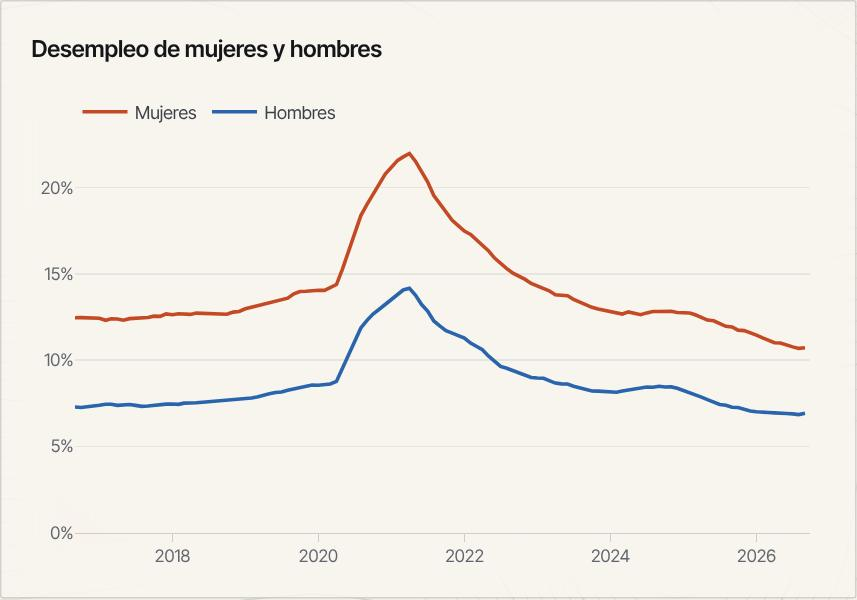
\includegraphics[width=\linewidth,height=0.42\textheight,keepaspectratio]{fig/g-emp-genero-td.jpg}\end{center}
\paragraph{Qué nos cuenta}
Compara la tasa de desempleo de las mujeres y la de los hombres en el total nacional. Muestra una de las brechas más persistentes del mercado laboral colombiano: el desempleo femenino ha estado de forma sistemática por encima del masculino. Permite ver si esa brecha se cierra o se amplía con el tiempo y cómo reaccionó cada grupo a los choques, como la pandemia de 2020.

\begin{leer}[Cómo se lee]
Eje vertical en porcentaje, desde cero; eje horizontal desde 2011. Línea naranja = mujeres; línea azul = hombres. Cada punto es el promedio de las tasas mensuales de los últimos 12 meses, sin desestacionalizar: promediar un año completo elimina la estacionalidad sin usar modelos estadísticos. La distancia vertical entre las dos líneas es la brecha de desempleo en puntos porcentuales.
\end{leer}

\paragraph{Por qué importa}
La brecha de género en el desempleo refleja barreras de acceso al empleo, la carga de cuidado no remunerado y la segmentación por sectores. Cerrarla amplía la oferta de trabajo efectiva, el ingreso de los hogares y el crecimiento potencial. Para un inversionista indica cuánto talento queda sin aprovechar y la profundidad del mercado de consumo.

\paragraph{Cómo interpretarlo}
\begin{itemize}
\item Si las dos líneas se acercan, la brecha se reduce; si se separan, se amplía.
\item Una caída del desempleo femenino puede deberse a que más mujeres consiguen trabajo o a que dejan de buscarlo; léalo con la participación laboral por sexo.
\item El promedio de 12 meses reacciona con rezago: un cambio brusco tarda varios meses en verse completo.
\item Al no estar desestacionalizada, la serie no es directamente comparable con la tasa de desempleo nacional desestacionalizada del primer gráfico.
\end{itemize}
\begin{formulas}[Fórmulas]
\formula{Tasa de desempleo por sexo}{TD\textsubscript{s,t} = D\textsubscript{s,t} $\div$ FT\textsubscript{s,t} $\times$ 100}{D = desocupados; FT = fuerza de trabajo; s = mujeres u hombres}
\formula{Promedio de 12 meses}{TD12\textsubscript{s,t} = (1 $\div$ 12) $\times$ $\Sigma$\textsubscript{k=0..11} TD\textsubscript{s,t−k}}{promedio simple de las tasas mensuales}
\formula{Brecha}{B\textsubscript{t} = TD12\textsubscript{mujeres,t} − TD12\textsubscript{hombres,t}}{en puntos porcentuales}
\end{formulas}
\begin{metodo}[Metodología]
Tasa de desocupación por sexo, total nacional, promedio móvil de 12 meses (elimina la estacionalidad sin modelos).
\par\smallskip{\small\textbf{Fuente:} DANE, Gran Encuesta Integrada de Hogares (GEIH), anexo mensual}
\end{metodo}

\subsection{Participación laboral de mujeres y hombres}
\label{g:g-emp-genero-tgp}
\begin{center}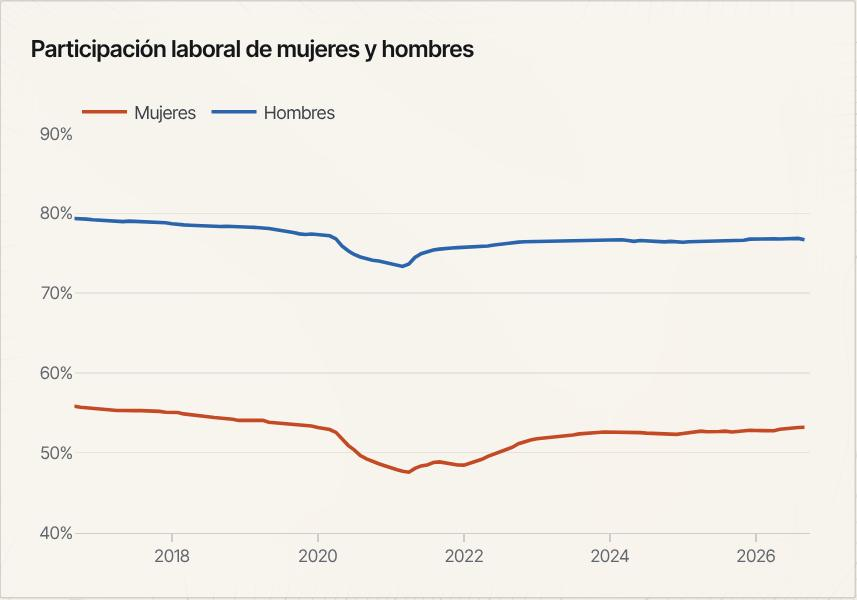
\includegraphics[width=\linewidth,height=0.42\textheight,keepaspectratio]{fig/g-emp-genero-tgp.jpg}\end{center}
\paragraph{Qué nos cuenta}
Compara la tasa global de participación (TGP) de mujeres y hombres: el porcentaje de las personas en edad de trabajar (15 años y más) que trabajan o buscan trabajo. Muestra que una proporción mucho menor de mujeres participa en el mercado laboral, en buena medida por el trabajo de cuidado y del hogar no remunerado, y si esa distancia cambia con el tiempo.

\begin{leer}[Cómo se lee]
Eje vertical en porcentaje, de 40\% a 90\% (no empieza en cero, para ver mejor los cambios); eje horizontal desde 2011. Línea naranja = mujeres; línea azul = hombres. Cada punto es el promedio de las tasas mensuales de los últimos 12 meses, sin desestacionalizar. La distancia vertical entre ambas líneas es la brecha de participación en puntos porcentuales.
\end{leer}

\paragraph{Por qué importa}
La participación laboral determina cuánta mano de obra está disponible para producir. La baja participación femenina es una de las principales fuentes de crecimiento potencial no aprovechado en Colombia: cada punto adicional amplía la fuerza de trabajo y el ingreso de los hogares. Para un inversionista ayuda a entender la oferta laboral, el consumo y la dinámica demográfica del país.

\paragraph{Cómo interpretarlo}
\begin{itemize}
\item Una TGP femenina en aumento con desempleo estable indica que más mujeres consiguen empleo; si sube junto con el desempleo, entran más de las que el mercado absorbe.
\item La caída de 2020 refleja salidas masivas de la fuerza de trabajo, mayores entre las mujeres, que no aparecen como desempleo.
\item Una participación más baja puede deberse a más años de estudio (positivo) o a más oficios del hogar; el gráfico de población fuera de la fuerza de trabajo muestra la razón.
\item El eje recortado amplía visualmente las diferencias; lea siempre los valores del eje.
\end{itemize}
\begin{formulas}[Fórmulas]
\formula{Tasa global de participación}{TGP\textsubscript{s,t} = FT\textsubscript{s,t} $\div$ PET\textsubscript{s,t} $\times$ 100}{FT = fuerza de trabajo (ocupados + desocupados); PET = población en edad de trabajar (15 años y más); s = sexo}
\formula{Promedio de 12 meses}{TGP12\textsubscript{s,t} = (1 $\div$ 12) $\times$ $\Sigma$\textsubscript{k=0..11} TGP\textsubscript{s,t−k}}{promedio simple de las tasas mensuales}
\end{formulas}
\begin{metodo}[Metodología]
Tasa global de participación = fuerza de trabajo / población en edad de trabajar (15 años y más), por sexo, promedio móvil de 12 meses.
\par\smallskip{\small\textbf{Fuente:} DANE, Gran Encuesta Integrada de Hogares (GEIH), anexo mensual}
\end{metodo}

\section{¿Cómo les va a los jóvenes?}

\subsection{Desempleo juvenil (15 a 28 años)}
\label{g:g-emp-jovenes}
\begin{center}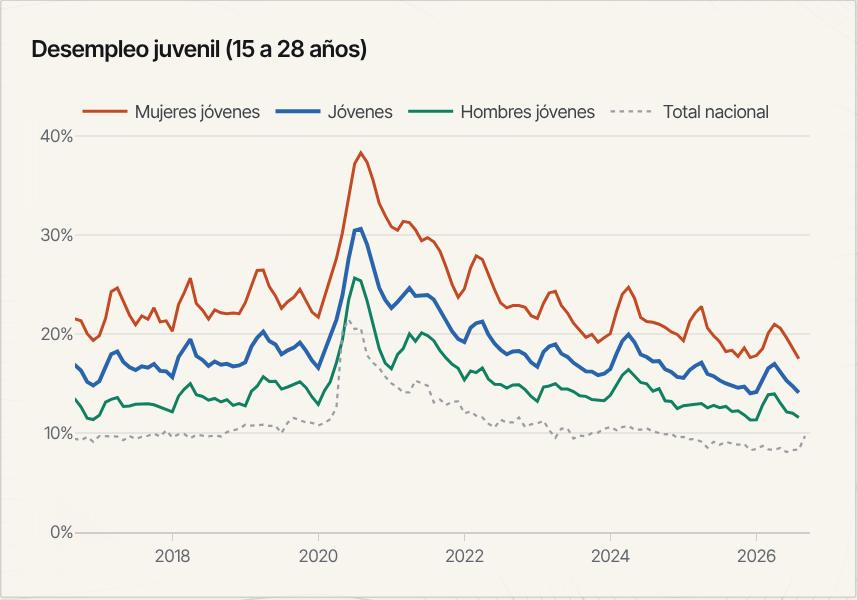
\includegraphics[width=\linewidth,height=0.42\textheight,keepaspectratio]{fig/g-emp-jovenes.jpg}\end{center}
\paragraph{Qué nos cuenta}
Muestra la tasa de desempleo de los jóvenes de 15 a 28 años (rango definido por la Ley 1622 de 2013, Estatuto de Ciudadanía Juvenil), en total y por sexo, frente al desempleo de toda la población. Revela que los jóvenes enfrentan tasas de desempleo muy superiores al promedio y que las mujeres jóvenes son el grupo más afectado.

\begin{leer}[Cómo se lee]
Eje vertical en porcentaje, desde cero; eje horizontal desde 2011. Línea azul gruesa = todos los jóvenes; naranja = mujeres jóvenes; verde = hombres jóvenes. Las series juveniles son trimestres móviles (tres meses que terminan en el mes indicado), sin desestacionalizar, del boletín de juventud de la GEIH. La línea gris punteada es la tasa de desempleo nacional mensual desestacionalizada, como referencia.
\end{leer}

\paragraph{Por qué importa}
El desempleo juvenil prolongado deja cicatrices duraderas: menor experiencia, salarios más bajos a lo largo de la vida y mayor probabilidad de informalidad. Afecta la acumulación de capital humano y la cohesión social. Para un inversionista es un indicador de la presión social y del aprovechamiento del bono demográfico del país.

\paragraph{Cómo interpretarlo}
\begin{itemize}
\item La distancia entre la línea azul y la gris mide cuánto peor les va a los jóvenes; una relación cercana a dos veces el promedio nacional es habitual en muchos países.
\item La separación entre la línea naranja y la verde es la brecha de género entre jóvenes, en general mayor que entre adultos.
\item Las series juveniles no están desestacionalizadas y la referencia sí: compare cada serie juvenil con el mismo trimestre de años anteriores, no mes a mes.
\item Los jóvenes que estudian y no buscan trabajo no cuentan como desempleados; complemente con el gráfico de jóvenes que ni estudian ni están ocupados.
\end{itemize}
\begin{formulas}[Fórmulas]
\formula{Tasa de desempleo juvenil}{TD\textsuperscript{J}\textsubscript{t} = D\textsuperscript{J}\textsubscript{t} $\div$ FT\textsuperscript{J}\textsubscript{t} $\times$ 100}{D\textsuperscript{J} = desocupados de 15 a 28 años; FT\textsuperscript{J} = fuerza de trabajo de 15 a 28 años; trimestre móvil terminado en t}
\end{formulas}
\begin{metodo}[Metodología]
Tasa de desocupación de las personas de 15 a 28 años (Ley 1622 de 2013), trimestre móvil. La referencia nacional es la serie desestacionalizada mensual.
\par\smallskip{\small\textbf{Fuente:} DANE, GEIH: mercado laboral de la juventud (15 a 28 años)}
\end{metodo}

\subsection{Jóvenes que ni estudian ni están ocupados}
\label{g:g-emp-nini}
\begin{center}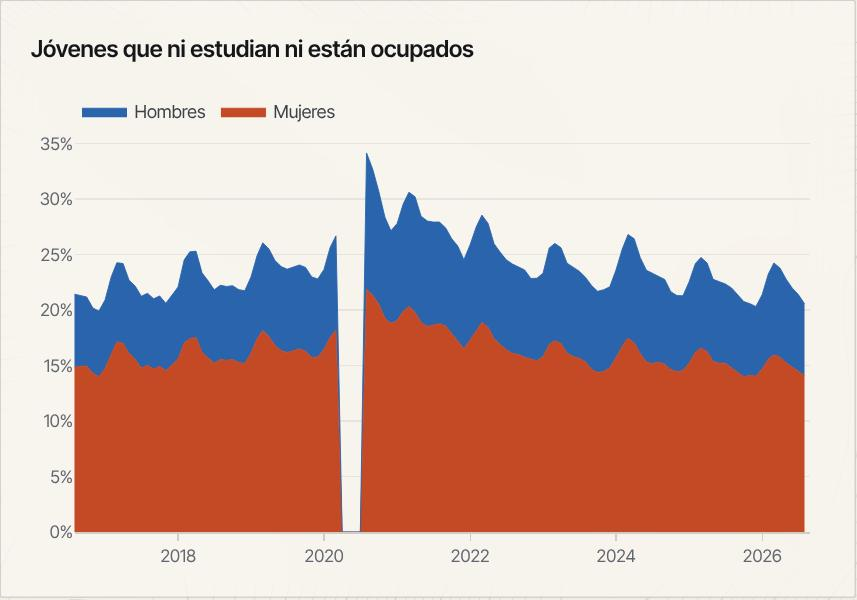
\includegraphics[width=\linewidth,height=0.42\textheight,keepaspectratio]{fig/g-emp-nini.jpg}\end{center}
\paragraph{Qué nos cuenta}
Muestra el porcentaje de jóvenes de 15 a 28 años que ni estudian ni están ocupados (conocidos como «ninis»), y cuánto de ese total corresponde a mujeres y cuánto a hombres. Es una medida más amplia de exclusión juvenil que el desempleo, porque incluye también a quienes no buscan trabajo, por ejemplo por dedicarse a oficios del hogar o por desaliento.

\begin{leer}[Cómo se lee]
Áreas apiladas en porcentaje del total de jóvenes de 15 a 28 años, desde 2011: la franja naranja (abajo) son las mujeres que ni estudian ni están ocupadas y la azul (arriba) los hombres; el borde superior es el total. Ambas franjas están expresadas sobre el total de jóvenes (no sobre los jóvenes de cada sexo), por eso se suman. Datos en trimestre móvil, sin desestacionalizar.
\end{leer}

\paragraph{Por qué importa}
Los jóvenes que no acumulan educación ni experiencia laboral pierden capital humano en la etapa de la vida en que más rinde, con efectos sobre su ingreso futuro y sobre la productividad del país. Una proporción alta también se asocia a mayor vulnerabilidad social. Para un inversionista, es un indicador del aprovechamiento del bono demográfico y de la calidad de la futura fuerza de trabajo.

\paragraph{Cómo interpretarlo}
\begin{itemize}
\item Si el área total se reduce, una mayor parte de los jóvenes estudia o trabaja.
\item La franja naranja suele ser bastante más ancha: muchas jóvenes están fuera del estudio y del empleo por labores de cuidado y del hogar.
\item Como es trimestre móvil sin desestacionalizar, compare con el mismo periodo de años anteriores (los ciclos académicos influyen).
\item Complemente con el desempleo juvenil y con la población fuera de la fuerza de trabajo.
\end{itemize}
\begin{formulas}[Fórmulas]
\formula{Proporción de ninis}{N\textsubscript{t} = J\textsuperscript{NEO}\textsubscript{t} $\div$ J\textsubscript{t} $\times$ 100}{J\textsuperscript{NEO} = jóvenes de 15 a 28 años que no estudian ni están ocupados; J = total de jóvenes de 15 a 28 años}
\formula{Descomposición por sexo}{N\textsubscript{t} = J\textsuperscript{NEO}\textsubscript{mujeres,t} $\div$ J\textsubscript{t} $\times$ 100 + J\textsuperscript{NEO}\textsubscript{hombres,t} $\div$ J\textsubscript{t} $\times$ 100}{cada franja se calcula sobre el total de jóvenes}
\end{formulas}
\begin{metodo}[Metodología]
Jóvenes de 15 a 28 años que no estudian ni están ocupados, como porcentaje del total de jóvenes; la serie de mujeres y la de hombres suman el total.
\par\smallskip{\small\textbf{Fuente:} DANE, GEIH: mercado laboral de la juventud (15 a 28 años)}
\end{metodo}

\section{Campo y ciudad, y quienes no participan}

\subsection{Desempleo en las cabeceras y en el campo}
\label{g:g-emp-area}
\begin{center}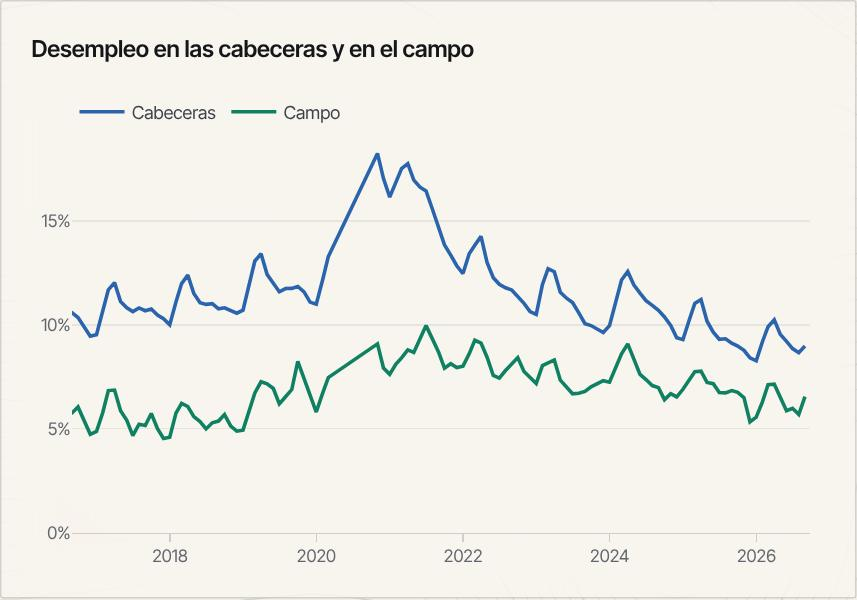
\includegraphics[width=\linewidth,height=0.42\textheight,keepaspectratio]{fig/g-emp-area.jpg}\end{center}
\paragraph{Qué nos cuenta}
Compara la tasa de desempleo en las cabeceras municipales (los cascos urbanos) con la de los centros poblados y el rural disperso (el campo). Muestra que el desempleo urbano es de forma persistente mayor que el rural, lo que no significa mejores condiciones en el campo: allí predominan el trabajo por cuenta propia, el agro y la informalidad.

\begin{leer}[Cómo se lee]
Eje vertical en porcentaje, desde cero; eje horizontal desde 2011. Línea azul = cabeceras; línea verde = campo (centros poblados y rural disperso). Cada punto es un trimestre móvil (tres meses que terminan en el mes indicado), sin desestacionalizar. La distancia vertical entre ambas líneas es la diferencia de desempleo entre ciudad y campo, en pp.
\end{leer}

\paragraph{Por qué importa}
La geografía del desempleo muestra dónde se concentra la holgura laboral y ayuda a entender el impacto regional del ciclo económico, de la construcción y de la industria (más urbanas) frente al agro (rural). Para un inversionista ayuda a dimensionar mercados de consumo urbanos y el riesgo social en las ciudades.

\paragraph{Cómo interpretarlo}
\begin{itemize}
\item Un desempleo rural bajo suele reflejar que en el campo casi todos trabajan en algo, aunque sea en actividades informales o de baja productividad; compárelo con la informalidad por sector.
\item El desempleo rural tiene estacionalidad marcada por las cosechas; compare con el mismo trimestre de años anteriores.
\item Las cabeceras concentran la mayor parte de la fuerza de trabajo, por lo que dominan el promedio nacional.
\item La muestra rural es más pequeña y su estimación es más volátil.
\end{itemize}
\begin{formulas}[Fórmulas]
\formula{Tasa de desempleo por zona}{TD\textsubscript{z,t} = D\textsubscript{z,t} $\div$ FT\textsubscript{z,t} $\times$ 100}{D = desocupados; FT = fuerza de trabajo; z = cabeceras o centros poblados y rural disperso; trimestre móvil terminado en t}
\formula{Diferencia ciudad−campo}{$\Delta$\textsubscript{t} = TD\textsubscript{cabeceras,t} − TD\textsubscript{campo,t}}{en puntos porcentuales}
\end{formulas}
\begin{metodo}[Metodología]
Tasa de desocupación en cabeceras y en centros poblados y rural disperso, trimestre móvil, sin desestacionalizar.
\par\smallskip{\small\textbf{Fuente:} DANE, Gran Encuesta Integrada de Hogares (GEIH), anexo mensual}
\end{metodo}

\subsection{¿Por qué no participan? Población fuera de la fuerza de trabajo}
\label{g:g-emp-fuera}
\begin{center}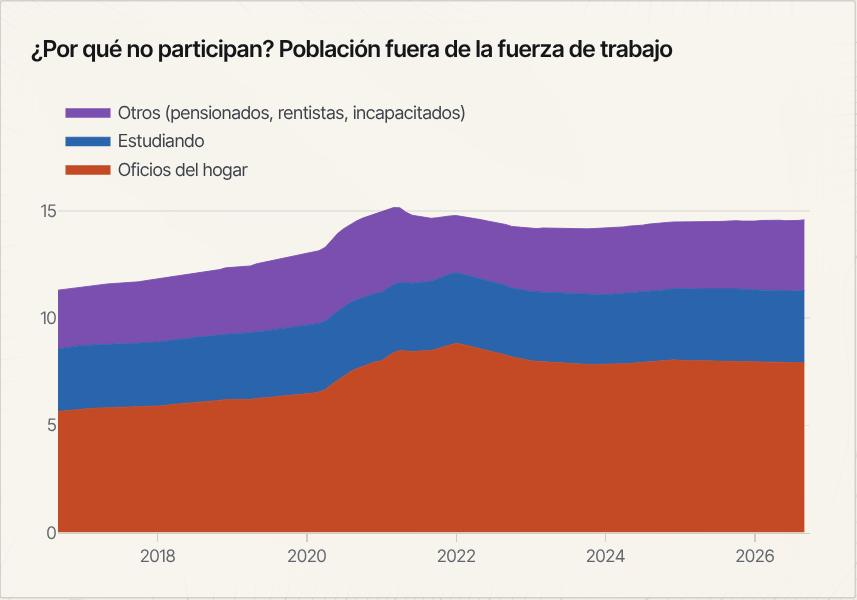
\includegraphics[width=\linewidth,height=0.42\textheight,keepaspectratio]{fig/g-emp-fuera.jpg}\end{center}
\paragraph{Qué nos cuenta}
Muestra cuántas personas en edad de trabajar no trabajan ni buscan trabajo, es decir, la población fuera de la fuerza de trabajo, y por qué: porque estudian, porque se dedican a oficios del hogar o por otras razones (pensionados, rentistas, personas con incapacidad permanente para trabajar). Ayuda a entender la otra cara de la tasa de participación.

\begin{leer}[Cómo se lee]
Áreas apiladas en millones de personas, total nacional, desde 2011. De abajo hacia arriba: naranja = oficios del hogar; azul = estudiando; morado = otros (pensionados, rentistas, incapacitados). El borde superior es el total de personas fuera de la fuerza de trabajo. Cada punto es el promedio de los últimos 12 meses de los datos mensuales, lo que elimina la estacionalidad.
\end{leer}

\paragraph{Por qué importa}
Una población inactiva grande reduce la oferta de trabajo disponible y la base de ingresos de la economía. Su composición importa: estudiar es una inversión en capital humano, mientras que una franja de oficios del hogar muy amplia, mayoritariamente femenina, indica barreras para incorporarse al empleo remunerado. Para un inversionista es clave para entender el potencial de crecimiento de la fuerza laboral.

\paragraph{Cómo interpretarlo}
\begin{itemize}
\item Si el total crece más rápido que la población en edad de trabajar, la participación laboral está cayendo.
\item Un aumento de la franja «estudiando» suele ser favorable; uno de «oficios del hogar» suele asociarse a labores de cuidado no remuneradas.
\item El envejecimiento de la población tiende a ampliar la franja de «otros» por el mayor número de pensionados.
\item El salto de 2020 refleja personas que dejaron de buscar trabajo durante la pandemia; compare con la participación por sexo.
\end{itemize}
\begin{formulas}[Fórmulas]
\formula{Población fuera de la fuerza de trabajo}{PFFT\textsubscript{t} = PET\textsubscript{t} − FT\textsubscript{t} = Est\textsubscript{t} + Hog\textsubscript{t} + Otr\textsubscript{t}}{PET = población en edad de trabajar; FT = fuerza de trabajo; Est, Hog, Otr = según actividad principal}
\formula{Promedio de 12 meses}{$\bar{\mathrm{X}}$\textsubscript{t} = (1 $\div$ 12) $\times$ $\Sigma$\textsubscript{k=0..11} X\textsubscript{t−k} $\div$ 1.000}{X = personas en cada categoría (miles); el resultado queda en millones}
\end{formulas}
\begin{metodo}[Metodología]
Población fuera de la fuerza de trabajo según su actividad principal (estudiando, oficios del hogar, otros), total nacional, promedio de 12 meses, en millones.
\par\smallskip{\small\textbf{Fuente:} DANE, Gran Encuesta Integrada de Hogares (GEIH), anexo mensual}
\end{metodo}

\section{Desempleo en las 32 capitales}

\subsection{Tasa de desempleo por ciudad capital, año móvil}
\label{g:g-cap-ciudades}
\begin{center}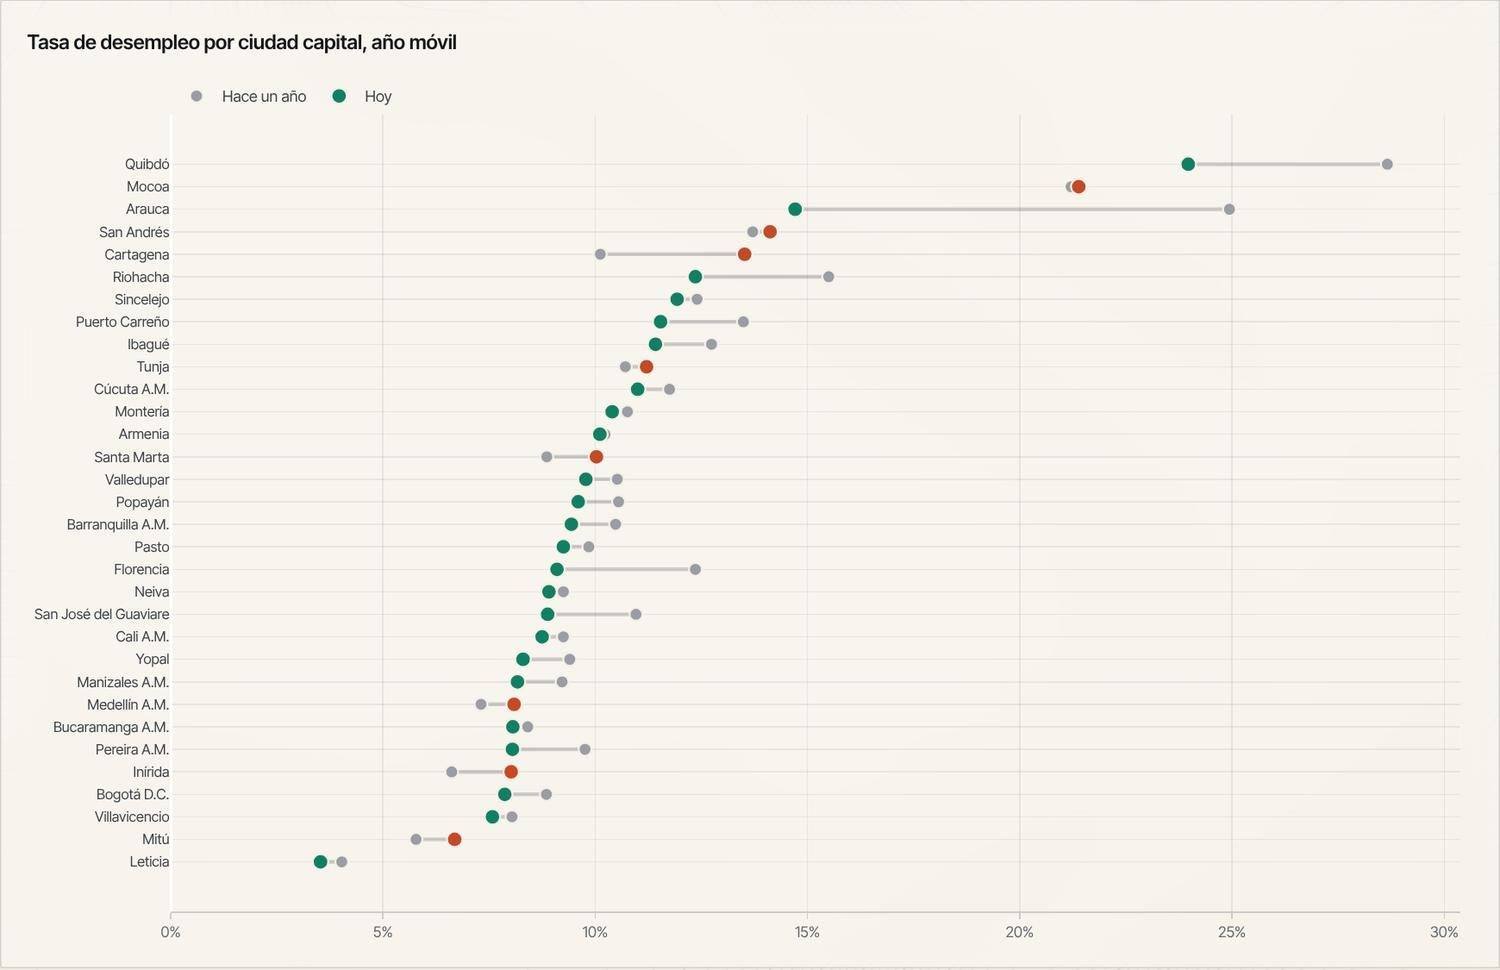
\includegraphics[width=\linewidth,height=0.42\textheight,keepaspectratio]{fig/g-cap-ciudades.jpg}\end{center}
\paragraph{Qué nos cuenta}
Compara la tasa de desempleo de las 32 ciudades capitales de departamento (13 de ellas con su área metropolitana) en el último año móvil, frente al año móvil terminado doce meses antes. Muestra la gran dispersión regional del desempleo en Colombia y en qué ciudades mejoró o empeoró en el último año.

\begin{leer}[Cómo se lee]
Cada fila es una ciudad, ordenada por su tasa más reciente (la más alta arriba); el eje horizontal está en porcentaje y empieza en cero. El punto gris es la tasa del año móvil terminado un año antes y el punto de color la del año móvil más reciente; la línea que los une muestra la magnitud del cambio. Punto verde: el desempleo bajó o no cambió; naranja: subió. Año móvil = promedio de los 12 meses que terminan en el último mes publicado.
\end{leer}

\paragraph{Por qué importa}
El desempleo urbano difiere mucho entre regiones según su estructura productiva, su grado de informalidad y su exposición a choques como la migración, el comercio fronterizo o los precios de las materias primas. Para un inversionista ayuda a identificar mercados laborales más holgados o más estrechos al decidir dónde ubicar operaciones, contratar o vender.

\paragraph{Cómo interpretarlo}
\begin{itemize}
\item Una línea larga entre el punto gris y el de color indica un cambio grande en el año; una línea corta, estabilidad.
\item Una tasa baja no siempre indica un mercado laboral sano: puede coincidir con alta informalidad o baja participación.
\item El año móvil elimina la estacionalidad y reduce el error de muestreo, pero reacciona con rezago a los cambios recientes.
\item Las ciudades pequeñas tienen muestras menores en la GEIH y cifras más volátiles; diferencias de 1 pp entre ellas pueden no ser significativas.
\end{itemize}
\begin{formulas}[Fórmulas]
\formula{Tasa de desempleo de la ciudad (año móvil)}{TD\textsubscript{c,t} = D\textsubscript{c} $\div$ FT\textsubscript{c} $\times$ 100}{D = desocupados; FT = fuerza de trabajo de la ciudad c en los 12 meses que terminan en t (cálculo del DANE)}
\formula{Cambio en un año}{$\Delta$TD\textsubscript{c} = TD\textsubscript{c,t} − TD\textsubscript{c,t−12}}{en pp; verde si $\Delta$TD $\le$ 0, naranja si $\Delta$TD > 0}
\end{formulas}
\begin{metodo}[Metodología]
Tasa de desocupación de cada una de las 32 ciudades capitales (13 con su área metropolitana), en año móvil de 12 meses, frente al año móvil terminado 12 meses antes.
\par\smallskip{\small\textbf{Fuente:} DANE, Gran Encuesta Integrada de Hogares (GEIH)}
\end{metodo}

\section*{Lecturas de la página}
\begin{itemize}\small
\item \textbf{OIT (2013). Resolución sobre las estadísticas del trabajo, la ocupación y la subutilización de la fuerza de trabajo. 19.ª CIET.} Definiciones de ocupación, desocupación, fuerza de trabajo y subutilización.
\item \textbf{OIT (1993). Resolución sobre la Clasificación Internacional de la Situación en el Empleo (CISE-93). 15.ª CIET.} Posiciones ocupacionales: asalariados, cuenta propia, empleadores, familiares.
\item \textbf{Maloney, W. F. (2004). Informality Revisited. World Development, 32(7), 1159–1178.} La informalidad y el trabajo por cuenta propia como elección y como segmentación.
\item \textbf{Goldin, C. (2014). A Grand Gender Convergence: Its Last Chapter. American Economic Review, 104(4), 1091–1119.} Brechas de participación y resultados laborales entre mujeres y hombres.
\item \textbf{Bell, D. N. F. y Blanchflower, D. G. (2011). Young People and the Great Recession. Oxford Review of Economic Policy, 27(2), 241–267.} Desempleo juvenil y cicatrices de largo plazo.
\item \textbf{DANE. Gran Encuesta Integrada de Hogares: metodología y marco conceptual (2021).} Fuente de todos los datos de esta página.
\end{itemize}

\chapter{Inflación}
\label{atlas:inflacion}

{\large\sffamily\bfseries Inflación y precios\par}\medskip

Cuánto suben los precios frente a la meta del Banco de la República, qué inflación espera el mercado y de dónde viene: divisiones, bienes y servicios, 188 subclases, niveles de ingreso y 23 ciudades.

{\small\color{cmmuted}Página del sitio: \url{https://stv-quant.github.io/ColombiaMacro-USBCali/inflacion/}}

\section{¿Cómo están los precios?}

\subsection{Inflación anual frente a la meta}
\label{g:g-inf}
\begin{center}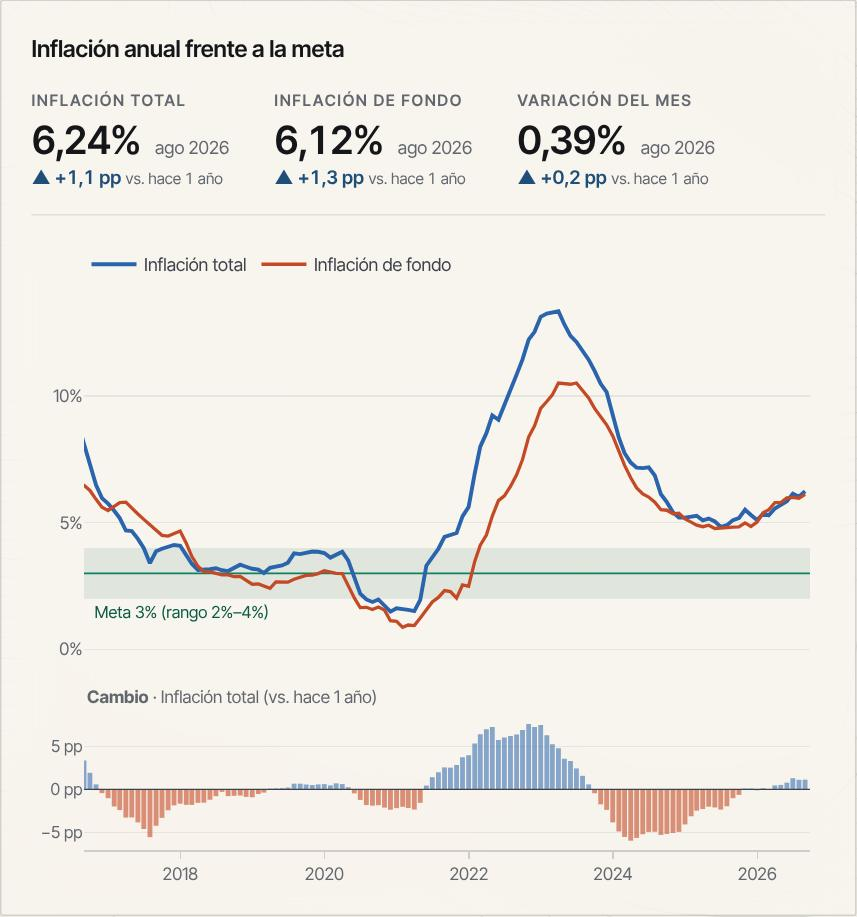
\includegraphics[width=\linewidth,height=0.42\textheight,keepaspectratio]{fig/g-inf.jpg}\end{center}
\paragraph{Qué nos cuenta}
Muestra la inflación anual de Colombia, medida con el Índice de Precios al Consumidor (IPC) del DANE, frente a la meta del Banco de la República, y la compara con la inflación de fondo, que excluye alimentos y precios regulados para aislar la presión persistente. Cuenta la historia de los ciclos de inflación: los choques que la alejan de la meta y el proceso de regreso.

\begin{leer}[Cómo se lee]
Panel superior, en \% anual: línea azul gruesa, inflación total; línea naranja, inflación sin alimentos ni regulados (cálculo del Banco de la República). La franja verde es el rango meta (2\% a 4\%) y la línea verde, la meta puntual de 3\%. Panel inferior: barras con el cambio de la inflación total frente al mismo mes del año anterior, en puntos porcentuales (pp); azules si subió y naranjas si bajó. La vista inicial abarca los últimos diez años; el recuadro flotante muestra el cambio anual de cada línea.
\end{leer}

\paragraph{Por qué importa}
La inflación erosiona el poder adquisitivo de salarios y ahorros, y es el objetivo principal del Banco de la República: cuando se aleja de la meta, el Banco ajusta su tasa de interés, lo que mueve el costo del crédito, la curva de TES y la tasa de cambio. Para un inversionista determina el rendimiento real de los activos en pesos y el ciclo de tasas.

\paragraph{Cómo interpretarlo}
\begin{itemize}
\item Línea azul por encima de la franja: la inflación supera el rango meta; dentro de ella, es coherente con el objetivo del Banco.
\item Si la línea naranja está por encima de la azul, la presión es de fondo (servicios, salarios, indexación) y suele ceder más despacio; si está por debajo, la inflación total la empujan alimentos o regulados.
\item Varias barras naranjas seguidas en el panel inferior indican desinflación; barras azules seguidas, que la inflación se acelera.
\item La inflación anual compara con el mismo mes del año anterior, de modo que un alza o una caída fuerte de hace doce meses produce efectos base cuando sale del cálculo.
\end{itemize}
\begin{formulas}[Fórmulas]
\formula{Inflación anual}{$\pi$\textsubscript{t} = (IPC\textsubscript{t} $\div$ IPC\textsubscript{t−12} − 1) $\times$ 100}{IPC\textsubscript{t} = índice de precios al consumidor del mes t (base diciembre 2018 = 100)}
\formula{Cambio anual (panel inferior)}{$\Delta\pi$\textsubscript{t} = $\pi$\textsubscript{t} − $\pi$\textsubscript{t−12}}{en pp}
\end{formulas}
\begin{metodo}[Metodología]
Inflación anual = variación del IPC en 12 meses. Inflación de fondo = sin alimentos ni precios regulados (cálculo del Banco de la República). Franja verde: meta de 3\% $\pm$ 1 punto.
\par\smallskip{\small\textbf{Fuente:} DANE, IPC; Banco de la República, inflación sin alimentos ni regulados}
\end{metodo}

\subsection{¿Qué precios suben más?}
\label{g:g-cp-barras}
\begin{center}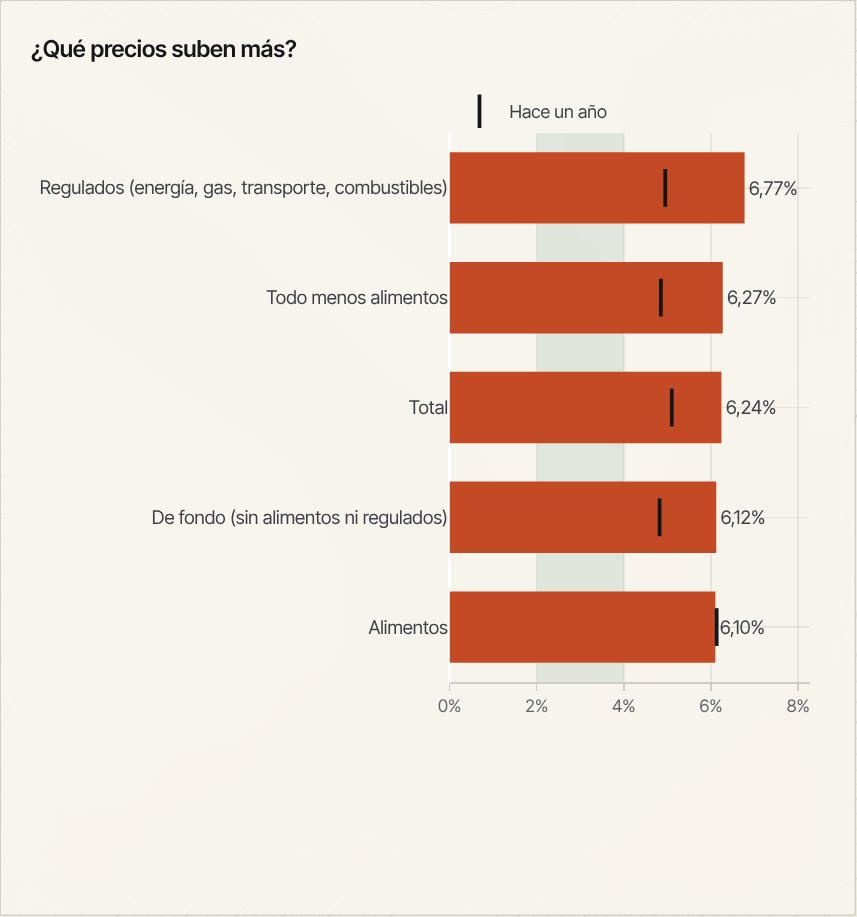
\includegraphics[width=\linewidth,height=0.42\textheight,keepaspectratio]{fig/g-cp-barras.jpg}\end{center}
\paragraph{Qué nos cuenta}
Compara la inflación anual más reciente de los grandes grupos de precios que sigue el Banco de la República: alimentos, regulados (energía, gas, transporte, combustibles y otros precios fijados o supervisados por el Estado), todo menos alimentos, la inflación de fondo (sin alimentos ni regulados) y el total. Muestra qué parte de la canasta presiona más y cómo ha cambiado frente a un año antes.

\begin{leer}[Cómo se lee]
Barras horizontales ordenadas de menor a mayor, en \% anual, con el valor rotulado al final. Las barras naranjas están por encima del techo del rango meta (4\%) y las azules en o por debajo de él. La franja verde vertical marca el rango meta (2\% a 4\%). La raya vertical negra sobre cada barra es el dato del mismo grupo doce meses antes: si la barra termina a la derecha de la raya, la inflación del grupo aumentó en el año. Corresponde al último mes publicado.
\end{leer}

\paragraph{Por qué importa}
No toda la inflación responde igual a la política monetaria: alimentos y regulados dependen del clima, de los precios internacionales y de decisiones administrativas, mientras que la inflación de fondo refleja la demanda y la indexación de precios y salarios, que es lo que la tasa del Banco busca moderar. Saber qué grupo explica la inflación ayuda a evaluar su persistencia.

\paragraph{Cómo interpretarlo}
\begin{itemize}
\item Si la inflación de fondo está en naranja, la presión no se limita a choques de oferta y suele tardar más en ceder.
\item Alimentos o regulados muy por encima del total indican un choque concentrado; su efecto en la inflación anual tiende a reducirse cuando el choque cumple doce meses.
\item Barra a la izquierda de su raya: el grupo se desinfló en el año; a la derecha, se aceleró.
\item Los grupos se solapan (el total contiene a todos y «todo menos alimentos» contiene a regulados), por lo que no suman ni se promedian entre sí.
\end{itemize}
\begin{formulas}[Fórmulas]
\formula{Inflación anual del grupo}{$\pi$\textsubscript{g,t} = (I\textsubscript{g,t} $\div$ I\textsubscript{g,t−12} − 1) $\times$ 100}{I\textsubscript{g,t} = índice de precios del grupo g en el último mes publicado t}
\formula{Raya de hace un año}{$\pi$\textsubscript{g,t−12}}{mismo cálculo doce meses antes}
\end{formulas}
\begin{metodo}[Metodología]
Variación anual del índice de precios de cada grupo en el último mes publicado; la raya es el mismo dato 12 meses antes. Los grupos se solapan (el total contiene a todos), por eso no suman.
\par\smallskip{\small\textbf{Fuente:} Banco de la República (IPC por grupos: alimentos, regulados, sin alimentos, sin alimentos ni regulados) y DANE, IPC}
\end{metodo}

\subsection{Inflación por grupo de precios en el tiempo}
\label{g:g-cp-lineas}
\begin{center}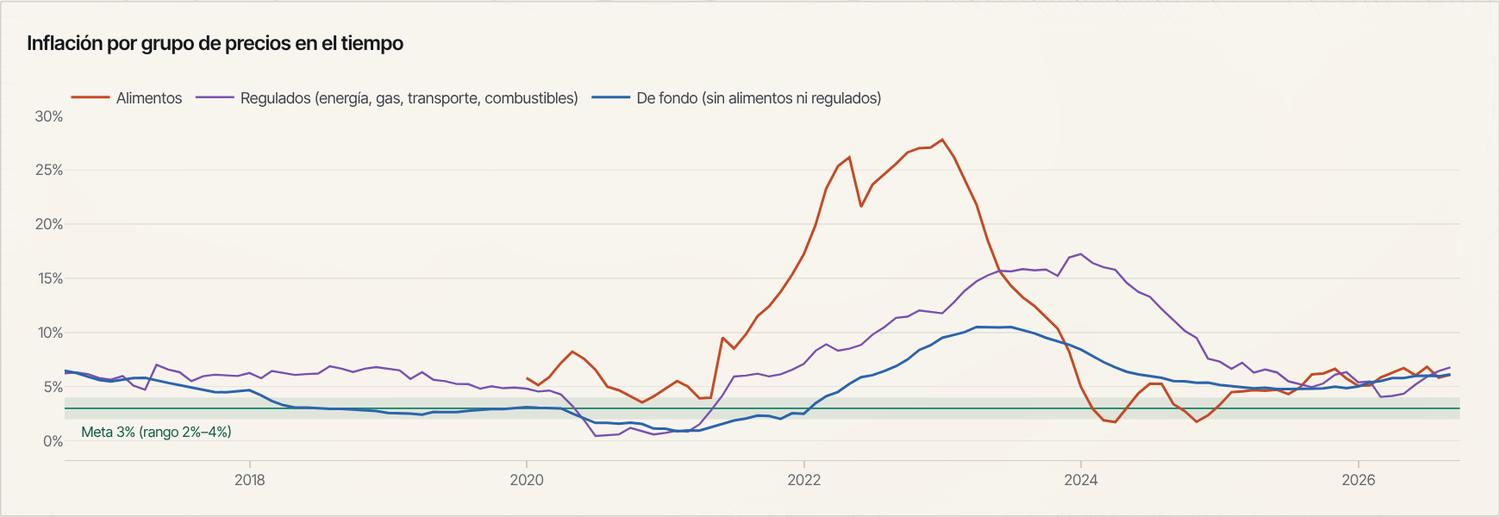
\includegraphics[width=\linewidth,height=0.42\textheight,keepaspectratio]{fig/g-cp-lineas.jpg}\end{center}
\paragraph{Qué nos cuenta}
Sigue en el tiempo la inflación anual de tres grupos de precios: alimentos, regulados y la inflación de fondo (sin alimentos ni regulados). Permite ver cómo los choques de alimentos y de precios regulados suben y bajan con rapidez, mientras la inflación de fondo se mueve más despacio y refleja la presión persistente que el Banco de la República busca controlar con su tasa de interés.

\begin{leer}[Cómo se lee]
Eje horizontal: fecha; eje vertical: inflación anual en \%. Línea naranja: alimentos; línea morada: regulados (servicios públicos, combustibles, transporte y otros precios fijados por el Estado); línea azul: inflación de fondo. La franja verde es el rango meta (2\% a 4\%) y la línea verde, la meta de 3\%. Datos mensuales con vista inicial de los últimos diez años; el recuadro flotante muestra el valor de cada grupo y su cambio frente a un año antes en pp.
\end{leer}

\paragraph{Por qué importa}
Distinguir choques transitorios de presiones persistentes es central para leer las decisiones de política monetaria: el Banco puede tolerar un choque de alimentos que se revierte, pero responde con más fuerza cuando la inflación de fondo se aleja de la meta. Para un inversionista, la trayectoria de la línea azul es una guía sobre la persistencia de la inflación y del ciclo de tasas.

\paragraph{Cómo interpretarlo}
\begin{itemize}
\item Picos de la línea naranja suelen asociarse a fenómenos climáticos (El Niño, La Niña) o a la tasa de cambio; tienden a revertirse en meses.
\item La línea morada refleja ajustes de tarifas de energía, gas, combustibles y transporte, a veces decididos por el Gobierno y escalonados en el tiempo.
\item Una línea azul que se mantiene por encima de 4\% indica presión de fondo amplia; cuando gira a la baja, la desinflación es más sólida.
\item Los choques en alimentos y regulados pueden contagiar a la inflación de fondo con rezago, por la indexación de salarios, arriendos y contratos a la inflación pasada.
\end{itemize}
\begin{formulas}[Fórmulas]
\formula{Inflación anual del grupo}{$\pi$\textsubscript{g,t} = (I\textsubscript{g,t} $\div$ I\textsubscript{g,t−12} − 1) $\times$ 100}{I\textsubscript{g,t} = índice de precios del grupo g en el mes t}
\formula{Cambio anual (recuadro)}{$\Delta\pi$\textsubscript{g,t} = $\pi$\textsubscript{g,t} − $\pi$\textsubscript{g,t−12}}{en pp}
\end{formulas}
\begin{metodo}[Metodología]
Variación anual mensual de cada grupo. Regulados: servicios públicos, combustibles, transporte y educación con precio fijado por el Estado.
\par\smallskip{\small\textbf{Fuente:} Banco de la República, inflación por grupos de precios}
\end{metodo}

\subsection{¿Qué inflación espera el mercado para el próximo año?}
\label{g:g-espera}
\begin{center}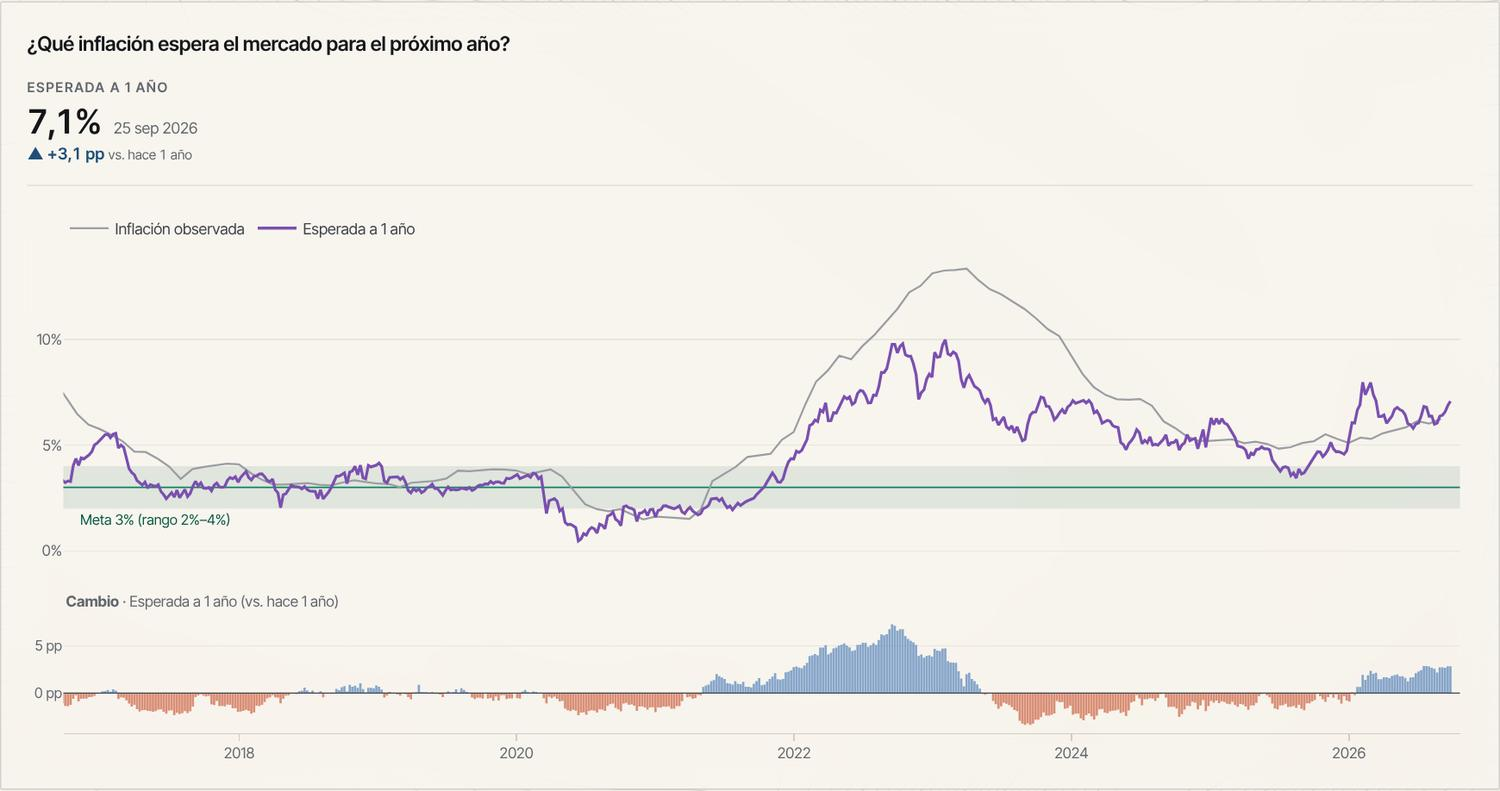
\includegraphics[width=\linewidth,height=0.42\textheight,keepaspectratio]{fig/g-espera.jpg}\end{center}
\paragraph{Qué nos cuenta}
Muestra la inflación que el mercado de deuda pública incorpora para los próximos doce meses (inflación de equilibrio o breakeven a 1 año) y la compara con la inflación observada. Se obtiene de los TES: la diferencia entre los que pagan una tasa fija en pesos y los que pagan una tasa real sobre la UVR, que se ajusta con la inflación. Es una medida diaria de expectativas basada en precios de mercado, no en encuestas.

\begin{leer}[Cómo se lee]
Panel superior, en \% anual: línea morada, inflación esperada a 1 año (serie semanal, último dato de cada viernes); línea gris, inflación anual observada del IPC (mensual). La franja verde es el rango meta (2\% a 4\%) y la línea verde, la meta de 3\%. Panel inferior: barras con el cambio de la inflación esperada a 1 año frente a un año antes, en pp; azules si subió y naranjas si bajó. La vista inicial abarca los últimos diez años.
\end{leer}

\paragraph{Por qué importa}
Las expectativas de inflación influyen en la fijación de salarios, arriendos y precios, y por eso el Banco de la República las sigue de cerca: si se alejan de la meta, la inflación tiende a volverse más persistente. Para un inversionista, comparar la expectativa con la inflación actual indica qué desinflación ya incorpora el mercado y sirve para elegir entre TES en pesos y TES UVR.

\paragraph{Cómo interpretarlo}
\begin{itemize}
\item Línea morada por encima de la franja verde: el mercado incorpora una inflación superior al rango meta para el próximo año; dentro de ella, coherente con la meta.
\item Línea morada por debajo de la gris: el mercado incorpora que la inflación será menor que la actual; por encima, mayor.
\item La medida incluye una prima por riesgo inflacionario (la eleva) y una prima por la menor liquidez de los TES UVR (tiende a reducirla), así que no es la expectativa pura.
\item El plazo de 1 año es sensible a datos mensuales de inflación y a la indexación de la UVR, que usa la inflación del mes anterior; conviene contrastarla con la Encuesta de Expectativas del Banco de la República.
\end{itemize}
\begin{formulas}[Fórmulas]
\formula{Breakeven a 1 año}{b\textsubscript{1} = [(1 + y\textsubscript{1}\textsuperscript{\$}) $\div$ (1 + r\textsubscript{1}) − 1] $\times$ 100}{y\textsubscript{1}\textsuperscript{\$} = tasa cero cupón TES en pesos a 1 año; r\textsubscript{1} = tasa cero cupón TES UVR a 1 año (tanto por uno)}
\formula{Cambio anual (panel inferior)}{$\Delta$b\textsubscript{1,t} = b\textsubscript{1,t} − b\textsubscript{1,t−1 año}}{en pp}
\end{formulas}
\begin{metodo}[Metodología]
Inflación esperada a 1 año (breakeven) = (1 + tasa TES en pesos) / (1 + tasa TES en UVR) − 1. Incluye primas por riesgo y liquidez, por lo que es una cota de la expectativa pura.
\par\smallskip{\small\textbf{Fuente:} Banco de la República, curvas cero cupón de los TES (series 15272–15277)}
\end{metodo}

\subsection{La inflación que el mercado espera para los próximos 10 años}
\label{g:g-tray}
\begin{center}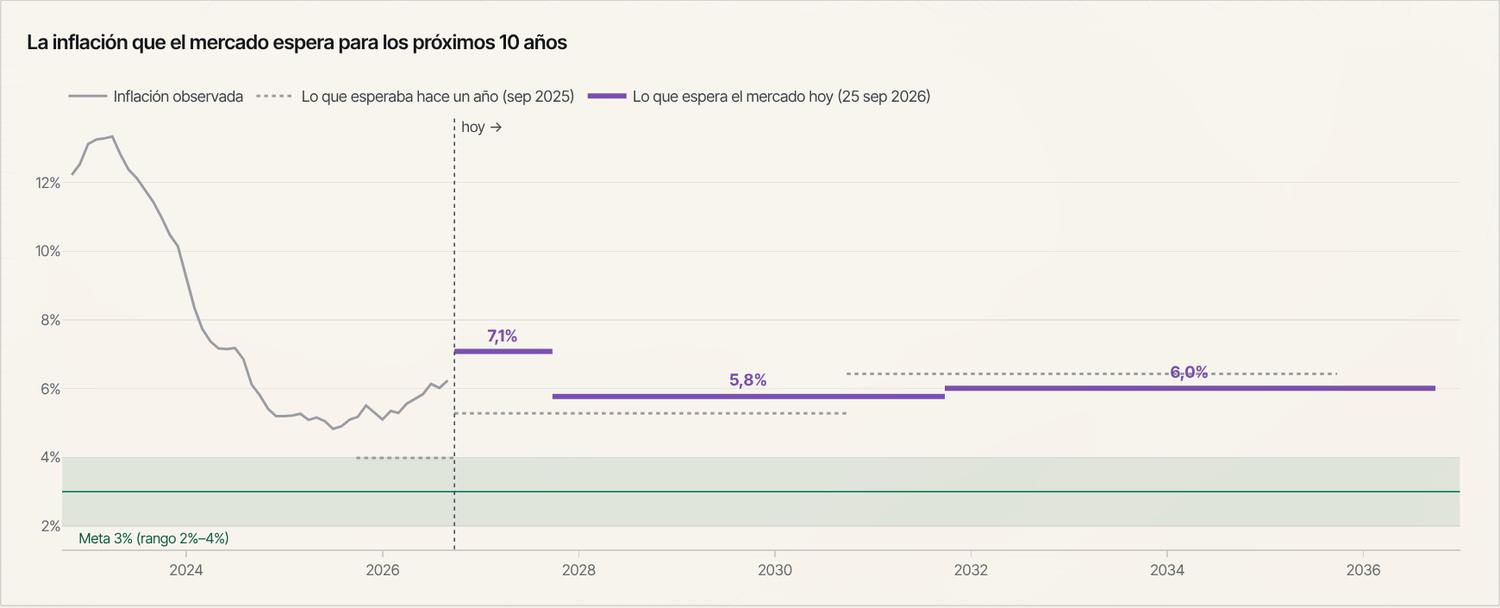
\includegraphics[width=\linewidth,height=0.42\textheight,keepaspectratio]{fig/g-tray.jpg}\end{center}
\paragraph{Qué nos cuenta}
Une en una misma línea de tiempo la inflación que ya ocurrió y la que hoy incorporan los precios de los TES para los próximos diez años, dividida en tres tramos: el próximo año, los años 1 a 5 y los años 5 a 10. Los tramos se obtienen de las inflaciones de equilibrio (breakeven) a 1, 5 y 10 años, encadenadas para aislar la inflación promedio de cada periodo futuro. Es la lectura del mercado, no una estimación propia del tablero.

\begin{leer}[Cómo se lee]
Eje horizontal: tiempo calendario, desde cuatro años atrás hasta diez años adelante; eje vertical: inflación anual en \%. A la izquierda de la línea vertical punteada («hoy»), la línea gris es la inflación anual observada del IPC. A la derecha, los tres escalones morados gruesos son la inflación promedio por año que incorporan los TES en cada tramo, con su valor rotulado. Los escalones grises punteados son la misma lectura hecha hace un año, ubicados desde esa fecha. La franja verde es el rango meta (2\% a 4\%) y la línea verde, la meta de 3\%.
\end{leer}

\paragraph{Por qué importa}
La forma de esta trayectoria resume cuánto tiempo cree el mercado que tomará el regreso de la inflación a la meta y dónde ubica la inflación de largo plazo, información clave para valorar activos en pesos, contratos indexados y deuda de largo plazo. Comparar con la lectura de hace un año muestra si la confianza en la desinflación ha mejorado o empeorado.

\paragraph{Cómo interpretarlo}
\begin{itemize}
\item Escalones que descienden hacia la franja verde: el mercado incorpora una convergencia gradual a la meta; escalones planos por encima de 4\% indican expectativas altas y persistentes.
\item Escalones morados por encima de los grises: el mercado incorpora hoy más inflación que hace un año para los mismos horizontes; por debajo, menos.
\item El tramo de 5 a 10 años (la «5y5y») es el más usado para medir el anclaje de largo plazo; su historia está en el gráfico «Inflación esperada a largo plazo».
\item Cada tramo incluye primas por riesgo inflacionario y por liquidez; los tramos encadenados reproducen exactamente el breakeven a 10 años, pero no son expectativas puras.
\end{itemize}
\begin{formulas}[Fórmulas]
\formula{Año 1}{f\textsubscript{0,1} = b\textsubscript{1}}{b\textsubscript{n} = breakeven a n años = (1 + y\textsubscript{n}\textsuperscript{\$}) $\div$ (1 + r\textsubscript{n}) − 1}
\formula{Años 1 a 5}{f\textsubscript{1,5} = [(1 + b\textsubscript{5})\textsuperscript{5} $\div$ (1 + b\textsubscript{1})]\textsuperscript{1/4} − 1}{inflación promedio anual implícita entre el año 1 y el 5}
\formula{Años 5 a 10 (5y5y)}{f\textsubscript{5,10} = [(1 + b\textsubscript{10})\textsuperscript{10} $\div$ (1 + b\textsubscript{5})\textsuperscript{5}]\textsuperscript{1/5} − 1}{inflación promedio anual implícita entre el año 5 y el 10}
\formula{Encadenamiento}{(1 + f\textsubscript{0,1}) $\times$ (1 + f\textsubscript{1,5})\textsuperscript{4} $\times$ (1 + f\textsubscript{5,10})\textsuperscript{5} = (1 + b\textsubscript{10})\textsuperscript{10}}{los tres tramos reproducen el breakeven a 10 años}
\end{formulas}
\begin{metodo}[Metodología]
Tramos implícitos: año 1 = b1; años 1–5 = [(1+b5)\textasciicircum{}5/(1+b1)]\textasciicircum{}(1/4) − 1; años 5–10 = [(1+b10)\textasciicircum{}10/(1+b5)\textasciicircum{}5]\textasciicircum{}(1/5) − 1 (la «5y5y»). Encadenan exactamente el breakeven a 10 años.
\par\smallskip{\small\textbf{Fuente:} Banco de la República, curvas cero cupón de los TES (series 15272–15277)}
\end{metodo}

\subsection{Inflación esperada a largo plazo (años 5 a 10)}
\label{g:g-anclaje}
\begin{center}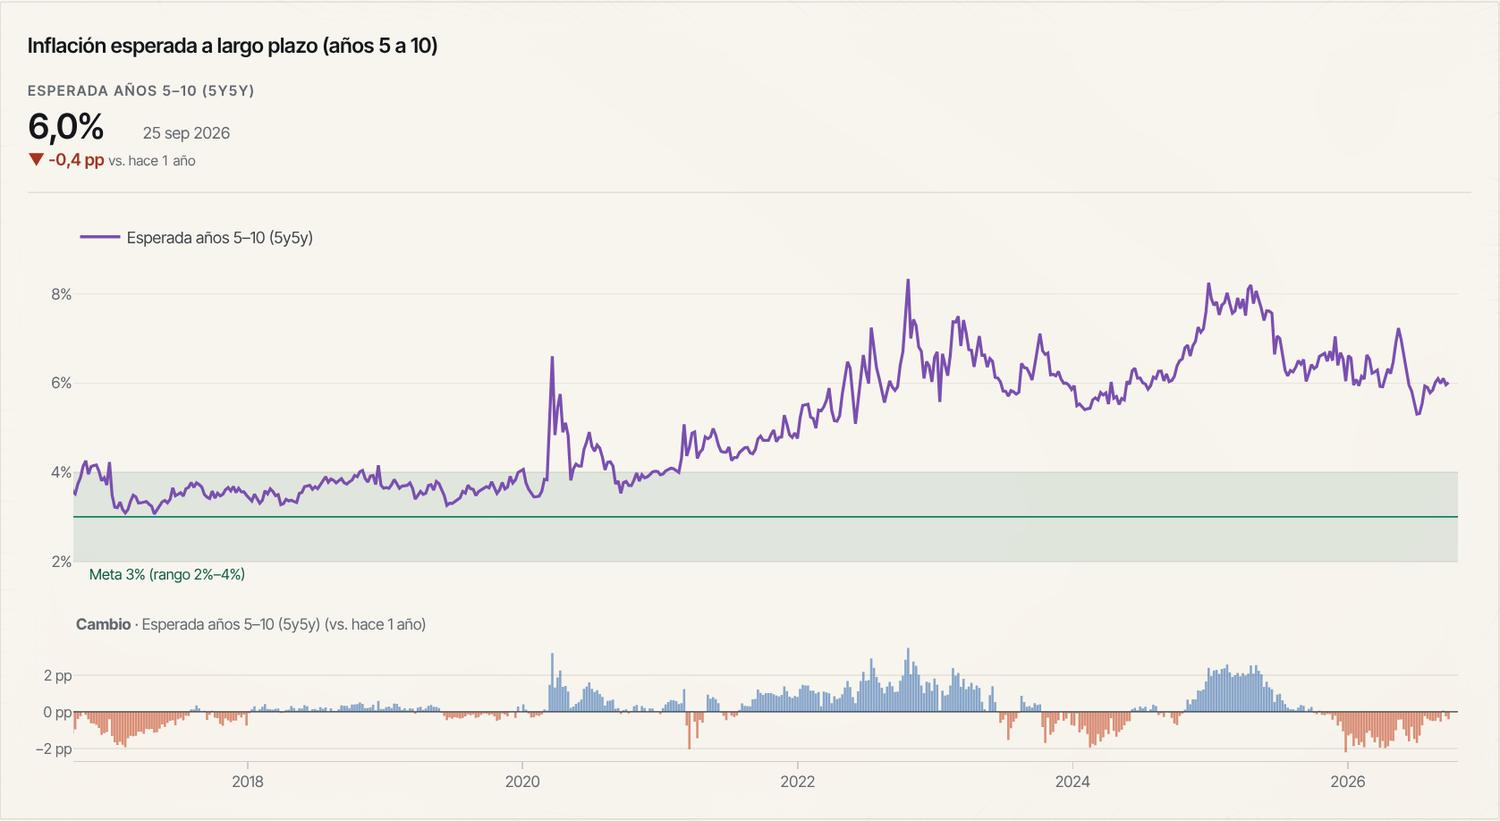
\includegraphics[width=\linewidth,height=0.42\textheight,keepaspectratio]{fig/g-anclaje.jpg}\end{center}
\paragraph{Qué nos cuenta}
Muestra la historia de la inflación que el mercado de TES incorpora, en promedio anual, para el periodo entre 5 y 10 años adelante (el forward 5y5y). Al mirar tan lejos, la medida deja de lado los choques transitorios de hoy y refleja la confianza en que el Banco de la República lleve la inflación a su meta de 3\% en el largo plazo: es la medida de mercado más usada del anclaje de las expectativas.

\begin{leer}[Cómo se lee]
Panel superior, en \% anual: la línea morada es el 5y5y semanal (último dato de cada viernes); cada punto es lo que el mercado incorporaba ese día para el tramo de 5 a 10 años adelante desde esa fecha. La franja verde es el rango meta (2\% a 4\%) y la línea verde, la meta de 3\%. Panel inferior: barras con el cambio del 5y5y frente a un año antes, en pp; azules si subió y naranjas si bajó. La vista inicial abarca los últimos diez años.
\end{leer}

\paragraph{Por qué importa}
Si las expectativas de largo plazo se mantienen ancladas a la meta, los choques de inflación tienden a disiparse sin contagiar salarios y precios, y el Banco necesita menos ajuste de tasas para controlarlos. Un desanclaje encarece la deuda de largo plazo y exige una política monetaria más restrictiva. Para un inversionista es una lectura directa de la credibilidad del Banco y de la prima por inflación en los TES largos.

\paragraph{Cómo interpretarlo}
\begin{itemize}
\item Cerca de 3\% y dentro de la franja: expectativas ancladas; por encima de 4\% el tablero las considera desancladas.
\item Si el 5y5y sube junto con la inflación observada, el mercado duda de que el choque sea transitorio; si se mantiene estable mientras la inflación sube, el anclaje funciona.
\item Barras azules persistentes en el panel inferior indican un deterioro gradual de la confianza de largo plazo.
\item Al ser un forward de largo plazo amplifica primas por riesgo inflacionario y por liquidez de los TES UVR, y es sensible a errores en las tasas a 5 y 10 años; los saltos aislados de un día se depuran.
\end{itemize}
\begin{formulas}[Fórmulas]
\formula{Forward 5y5y}{f\textsubscript{5,10} = [(1 + b\textsubscript{10})\textsuperscript{10} $\div$ (1 + b\textsubscript{5})\textsuperscript{5}]\textsuperscript{1/5} − 1}{b\textsubscript{n} = breakeven a n años = (1 + y\textsubscript{n}\textsuperscript{\$}) $\div$ (1 + r\textsubscript{n}) − 1}
\formula{Forma equivalente}{f\textsubscript{5,10} = F\textsuperscript{\$} $\div$ F\textsuperscript{UVR} − 1}{F = [(1 + y\textsubscript{10})\textsuperscript{10} $\div$ (1 + y\textsubscript{5})\textsuperscript{5}]\textsuperscript{1/5}, factor forward nominal (\$) o real (UVR)}
\formula{Cambio anual (panel inferior)}{$\Delta$f\textsubscript{t} = f\textsubscript{t} − f\textsubscript{t−1 año}}{en pp}
\end{formulas}
\begin{metodo}[Metodología]
Forward 5y5y = [(1+b10)\textasciicircum{}10/(1+b5)\textasciicircum{}5]\textasciicircum{}(1/5) − 1, último dato de cada semana. Mide la inflación que el mercado espera entre 5 y 10 años adelante.
\par\smallskip{\small\textbf{Fuente:} Banco de la República, curvas cero cupón de los TES (series 15272–15277)}
\end{metodo}

\section{¿Qué explica la inflación?}

\subsection{Aporte de cada división a la inflación anual (ago 2026)}
\label{g:g-inf-aportes}
\begin{center}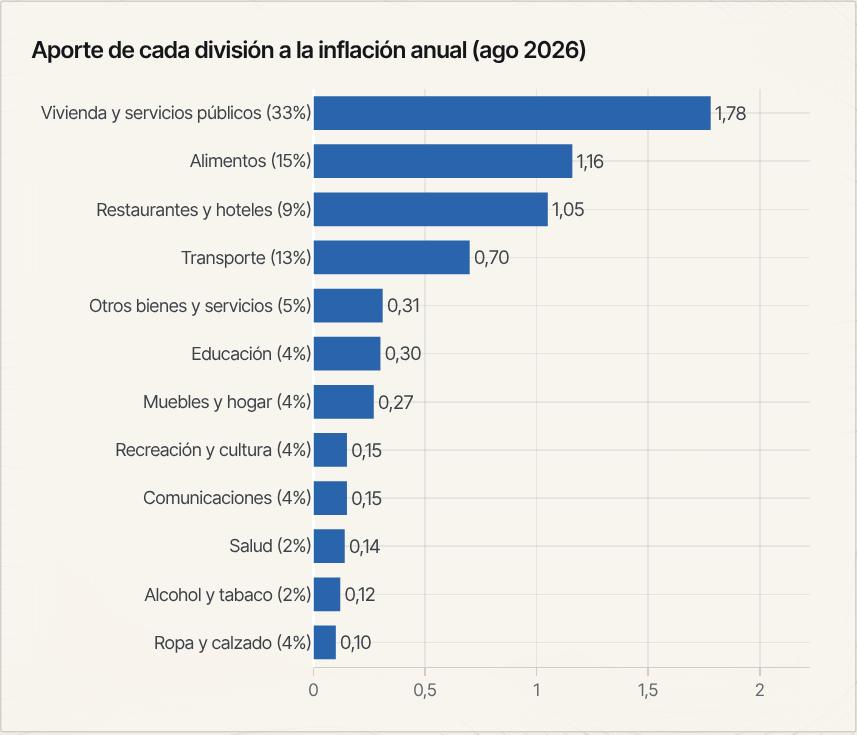
\includegraphics[width=\linewidth,height=0.42\textheight,keepaspectratio]{fig/g-inf-aportes.jpg}\end{center}
\paragraph{Qué nos cuenta}
Descompone la inflación anual total en el aporte de cada una de las 12 divisiones de gasto de la canasta del IPC (clasificación COICOP de Naciones Unidas: alimentos, vivienda y servicios públicos, transporte, restaurantes y hoteles, etc.). Combina cuánto suben los precios de cada división con cuánto pesa en el gasto de los hogares, y responde qué rubros explican la inflación del último mes publicado.

\begin{leer}[Cómo se lee]
Barras horizontales azules, ordenadas de menor a mayor aporte (el mayor arriba), con el valor rotulado en puntos porcentuales (pp). Entre paréntesis, junto al nombre de cada división, su ponderación en la canasta del IPC (en \% del gasto total). La suma de todas las barras es la inflación anual total. Una barra negativa indica una división cuyos precios bajaron y restan a la inflación. Corresponde al último mes publicado por el DANE.
\end{leer}

\paragraph{Por qué importa}
Una división puede subir mucho y aportar poco si pesa poco, o subir moderadamente y explicar buena parte de la inflación si pesa mucho, como vivienda (que incluye arriendos y servicios públicos) o alimentos. Identificar los aportes ayuda a evaluar si la inflación es de oferta (alimentos, energía) o de demanda y de indexación (servicios, arriendos), y por tanto su persistencia.

\paragraph{Cómo interpretarlo}
\begin{itemize}
\item Las divisiones con más peso (alimentos, vivienda, transporte) suelen dominar los aportes; un aporte grande de una división pequeña señala un choque fuerte de precios en ella.
\item Conviene leerlo con el gráfico vecino «Inflación anual de cada división»: aquel muestra cuánto suben los precios; este, cuánto pesa ese aumento en el total.
\item Si el aporte de vivienda es alto y estable, la inflación tiene un componente persistente asociado a arriendos e indexación.
\item El aporte usa el peso efectivo de cada división, que cambia con los precios relativos desde la base 2018; por eso no es exactamente la ponderación por la variación.
\end{itemize}
\begin{formulas}[Fórmulas]
\formula{Aporte de la división i}{A\textsubscript{i,t} = w\textsubscript{i} $\times$ (I\textsubscript{i,t−12} $\div$ I\textsubscript{t−12}) $\times$ $\pi$\textsubscript{i,t}}{w\textsubscript{i} = ponderación base 2018; I\textsubscript{i} = índice de la división; I = IPC total; $\pi$\textsubscript{i,t} = inflación anual de la división (\%)}
\formula{Suma de aportes}{$\Sigma$\textsubscript{i} A\textsubscript{i,t} = $\pi$\textsubscript{t}}{$\pi$\textsubscript{t} = inflación anual total; resultado en pp}
\end{formulas}
\begin{metodo}[Metodología]
Aporte de cada división (COICOP) a la variación anual del IPC total, calculado por el DANE con las ponderaciones de la canasta 2018 y la evolución de precios relativos.
\par\smallskip{\small\textbf{Fuente:} DANE, IPC base diciembre 2018 (anexos mensuales)}
\end{metodo}

\subsection{Inflación anual de cada división}
\label{g:g-inf-divisiones}
\begin{center}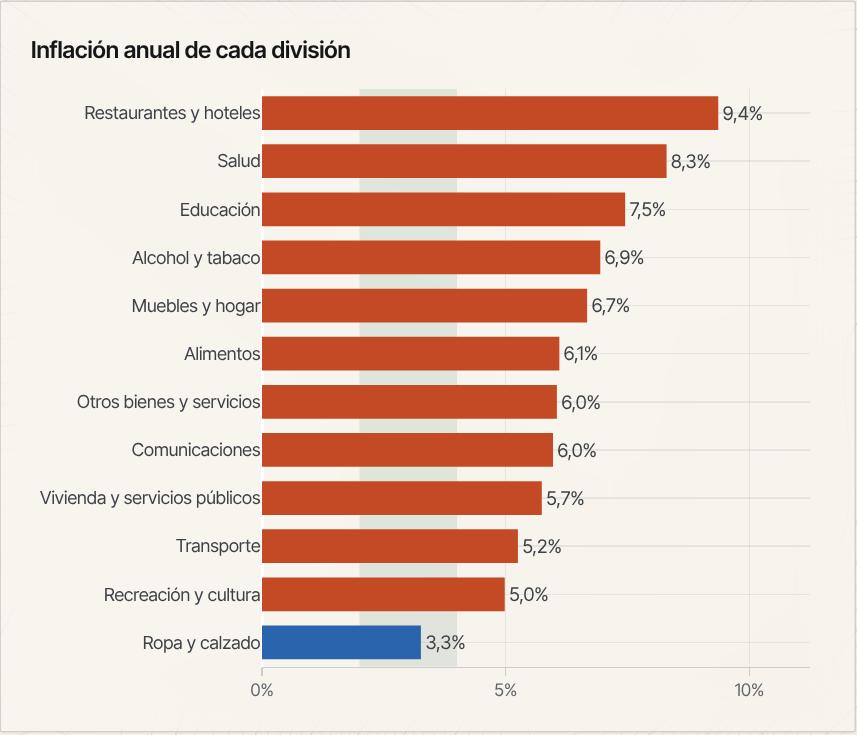
\includegraphics[width=\linewidth,height=0.42\textheight,keepaspectratio]{fig/g-inf-divisiones.jpg}\end{center}
\paragraph{Qué nos cuenta}
Compara la inflación anual de cada una de las 12 divisiones de gasto del IPC (clasificación COICOP): alimentos, alcohol y tabaco, ropa y calzado, vivienda y servicios públicos, muebles y hogar, salud, transporte, comunicaciones, recreación y cultura, educación, restaurantes y hoteles, y otros bienes y servicios. Muestra qué tan generalizada es la inflación entre los grandes rubros del gasto de los hogares en el último mes publicado.

\begin{leer}[Cómo se lee]
Barras horizontales ordenadas de menor a mayor inflación (la mayor arriba), en \% anual, con el valor rotulado. Las barras naranjas superan el techo del rango meta (4\%) y las azules están en o por debajo de él. La franja verde vertical marca el rango meta del Banco de la República (2\% a 4\%). Una barra a la izquierda de cero indica que los precios de esa división bajaron en el último año. Datos del total nacional.
\end{leer}

\paragraph{Por qué importa}
La dispersión entre divisiones revela la naturaleza de la inflación: si casi todas están en naranja, la presión es amplia y responde a la demanda y a la indexación; si solo unas pocas, se trata de choques sectoriales. Para empresas e inversionistas indica qué sectores enfrentan mayores aumentos de costos o tienen más poder para subir precios.

\paragraph{Cómo interpretarlo}
\begin{itemize}
\item Muchas barras naranjas: inflación generalizada; pocas barras naranjas con valores muy altos: choques concentrados.
\item Educación suele ajustarse una vez al año (a comienzos del año escolar) y salud con decisiones regulatorias, por lo que su inflación anual cambia en escalones.
\item La inflación de una división no dice cuánto aporta al total: para eso está el gráfico vecino «Aporte de cada división».
\item Las divisiones agrupan bienes muy distintos; el detalle por subclase está en los gráficos de difusión y de subclases que más suman y restan.
\end{itemize}
\begin{formulas}[Fórmulas]
\formula{Inflación anual de la división}{$\pi$\textsubscript{i,t} = (I\textsubscript{i,t} $\div$ I\textsubscript{i,t−12} − 1) $\times$ 100}{I\textsubscript{i,t} = índice de precios de la división i en el mes t (base diciembre 2018 = 100), total nacional}
\end{formulas}
\begin{metodo}[Metodología]
Variación anual del índice de cada división de gasto, total nacional.
\par\smallskip{\small\textbf{Fuente:} DANE, IPC base diciembre 2018 (anexos mensuales)}
\end{metodo}

\section{¿Suben más los bienes o los servicios?}

\subsection{Inflación de servicios y de bienes}
\label{g:g-inf-bienes-servicios}
\begin{center}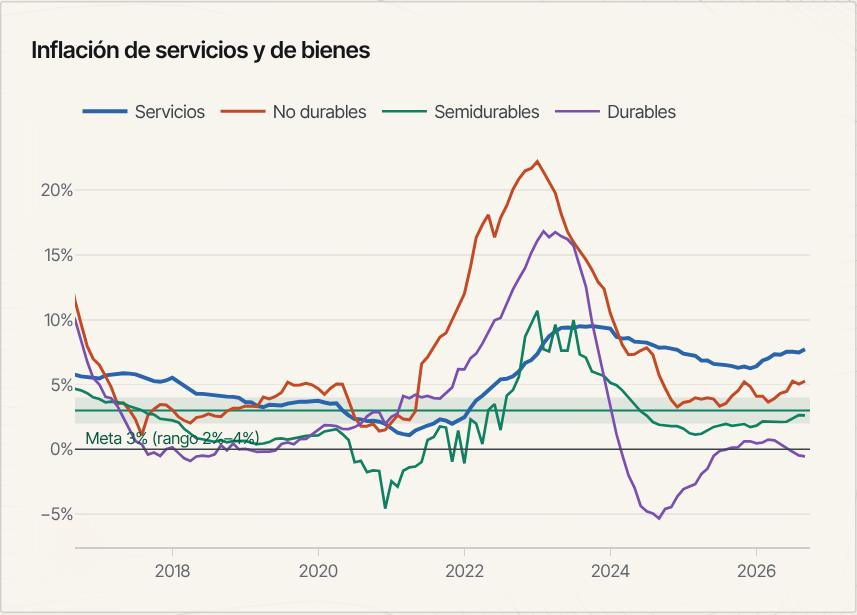
\includegraphics[width=\linewidth,height=0.42\textheight,keepaspectratio]{fig/g-inf-bienes-servicios.jpg}\end{center}
\paragraph{Qué nos cuenta}
Compara la inflación anual de los servicios con la de los bienes, separados por su durabilidad según la clasificación del DANE: no durables (alimentos, combustibles, aseo), semidurables (ropa, calzado, utensilios) y durables (vehículos, electrodomésticos, muebles). Cada grupo responde a fuerzas distintas, y su comparación ayuda a entender de dónde viene la inflación.

\begin{leer}[Cómo se lee]
Eje horizontal: fecha, desde 2012; eje vertical: variación anual en \%. Línea azul gruesa: servicios; línea naranja: bienes no durables; línea verde: semidurables; línea morada: durables. La franja verde es el rango meta (2\% a 4\%) con la línea de la meta de 3\%, y la línea horizontal gris marca el cero. Datos mensuales; el recuadro flotante muestra los cuatro valores a la vez.
\end{leer}

\paragraph{Por qué importa}
Los servicios dependen sobre todo de salarios, arriendos e indexación, por lo que su inflación es persistente y sensible a la demanda interna y al salario mínimo; los durables, en buena parte importados, se mueven con la tasa de cambio; los no durables, con alimentos y energía. Saber qué grupo lidera indica si la inflación responde más a la política monetaria o a choques externos y de oferta.

\paragraph{Cómo interpretarlo}
\begin{itemize}
\item Servicios por encima de los bienes por un periodo largo: presión de fondo ligada a salarios e indexación, que suele ceder despacio.
\item Durables al alza tras una depreciación del peso: transmisión de la tasa de cambio; su inflación puede ser negativa cuando el peso se aprecia o la demanda cae.
\item Los no durables reaccionan primero a choques de alimentos y combustibles y son los más volátiles.
\item Las series se calculan como variación anual de índices del DANE (base diciembre 2018 = 100); el inicio en 2012 permite comparar varios ciclos.
\end{itemize}
\begin{formulas}[Fórmulas]
\formula{Inflación anual por durabilidad}{$\pi$\textsubscript{k,t} = (I\textsubscript{k,t} $\div$ I\textsubscript{k,t−12} − 1) $\times$ 100}{I\textsubscript{k,t} = índice del DANE del grupo k (servicios, no durables, semidurables o durables) en el mes t}
\end{formulas}
\begin{metodo}[Metodología]
Índices del DANE por durabilidad (servicios, bienes durables, semidurables y no durables), base diciembre 2018 = 100; variación frente al mismo mes del año anterior.
\par\smallskip{\small\textbf{Fuente:} DANE, IPC base diciembre 2018 (anexos mensuales)}
\end{metodo}

\subsection{Energéticos frente a la inflación sin alimentos ni energéticos}
\label{g:g-inf-energia}
\begin{center}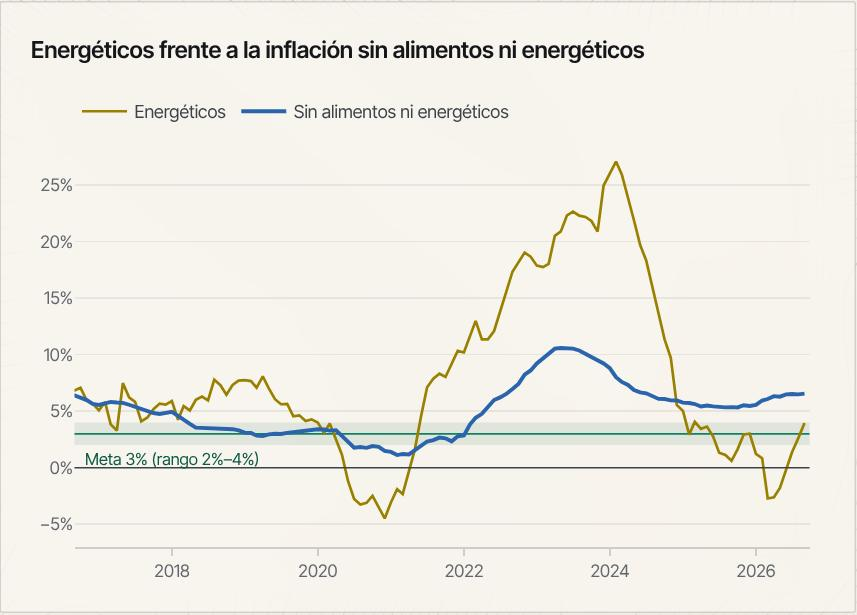
\includegraphics[width=\linewidth,height=0.42\textheight,keepaspectratio]{fig/g-inf-energia.jpg}\end{center}
\paragraph{Qué nos cuenta}
Contrasta la inflación de los energéticos (gas, energía eléctrica y combustibles) con la inflación sin alimentos ni energéticos, la medida de inflación básica más usada internacionalmente. Los energéticos son de los precios más volátiles de la canasta; la medida básica los excluye, junto con los alimentos, para mostrar la presión de precios persistente.

\begin{leer}[Cómo se lee]
Eje horizontal: fecha, desde 2012; eje vertical: variación anual en \%. Línea amarilla: energéticos; línea azul gruesa: IPC sin alimentos ni energéticos. La franja verde es el rango meta (2\% a 4\%) con la línea de la meta de 3\%, y la línea horizontal gris marca el cero. Para que los picos no aplasten el resto del gráfico, la línea de energéticos se recorta entre −20\% y 40\%. Datos mensuales del DANE.
\end{leer}

\paragraph{Por qué importa}
Los precios de la energía dependen del petróleo, del clima (que afecta la generación hidroeléctrica), de la tasa de cambio y de decisiones regulatorias sobre tarifas y combustibles. Separarlos de la inflación básica permite ver si un alza de la inflación total es un choque energético que puede revertirse o una presión generalizada que exige más respuesta de la política monetaria.

\paragraph{Cómo interpretarlo}
\begin{itemize}
\item Energéticos muy por encima de la línea azul: la inflación total la empuja un choque de energía; si la línea azul también sube, el choque se está transmitiendo al resto de precios.
\item Línea azul por encima de 4\% con energéticos estables: la presión es de fondo y no depende de la energía.
\item Los ajustes graduales de precios de combustibles o tarifas definidos por el Gobierno pueden mantener alta la inflación de energéticos por varios meses.
\item Esta medida básica (sin alimentos ni energéticos, del DANE) no es la misma que la inflación sin alimentos ni regulados del Banco de la República mostrada en «Inflación anual frente a la meta».
\end{itemize}
\begin{formulas}[Fórmulas]
\formula{Inflación anual}{$\pi$\textsubscript{k,t} = (I\textsubscript{k,t} $\div$ I\textsubscript{k,t−12} − 1) $\times$ 100}{I\textsubscript{k,t} = índice del DANE de energéticos o del IPC sin alimentos ni energéticos en el mes t}
\formula{Recorte visual}{$\pi$̃\textsubscript{E,t} = min(max($\pi$\textsubscript{E,t}, −20), 40)}{solo para la línea de energéticos (E)}
\end{formulas}
\begin{metodo}[Metodología]
IPC de energéticos (gas, energía eléctrica y combustibles) e IPC total sin alimentos ni energéticos, publicados por el DANE; variación anual.
\par\smallskip{\small\textbf{Fuente:} DANE, IPC base diciembre 2018 (anexos mensuales)}
\end{metodo}

\section{¿Qué tan generalizada es la inflación?}

\subsection{Distribución de la inflación anual entre 188 subclases (ago 2026)}
\label{g:g-inf-difusion}
\begin{center}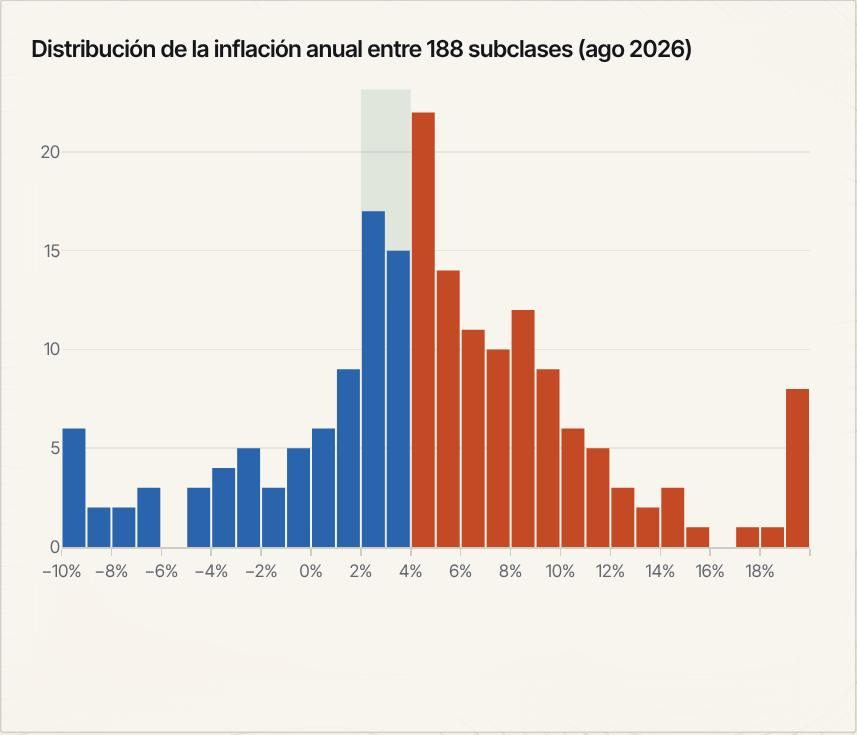
\includegraphics[width=\linewidth,height=0.42\textheight,keepaspectratio]{fig/g-inf-difusion.jpg}\end{center}
\paragraph{Qué nos cuenta}
Muestra cómo se reparte la inflación anual entre las 188 subclases de la canasta del IPC, el nivel más detallado que publica el DANE (por ejemplo arroz, arriendo, electricidad o comidas fuera del hogar). En lugar de un promedio, enseña la distribución completa: si la mayoría de precios suben a un ritmo parecido o si unos pocos suben mucho mientras el resto se mantiene estable.

\begin{leer}[Cómo se lee]
Histograma: el eje horizontal es la inflación anual en intervalos de 1 punto porcentual (de −10\% a 20\%) y el eje vertical, el número de subclases en cada intervalo. Las subclases no se ponderan: cada una cuenta igual. Las barras naranjas son los intervalos por encima de 4\% (el techo del rango meta) y las azules, los de 4\% o menos. La franja verde marca el rango meta (2\% a 4\%). Los valores extremos se acumulan en los intervalos de los bordes. Corresponde al último mes publicado.
\end{leer}

\paragraph{Por qué importa}
La difusión mide qué tan generalizada es la inflación, algo que el promedio no revela: una inflación del 6\% puede venir de unos pocos precios disparados o de un alza amplia de casi todos. Cuando la mayoría de subclases supera la meta, la inflación tiende a ser más persistente y la política monetaria más exigente; cuando la masa está en la franja verde, los focos son puntuales.

\paragraph{Cómo interpretarlo}
\begin{itemize}
\item Masa de barras a la derecha de 4\% (naranja): inflación generalizada; masa en la franja verde: la mayoría de precios es coherente con la meta.
\item Una distribución ancha indica gran dispersión de precios relativos, típica de choques de oferta; una estrecha, de presiones comunes como la indexación.
\item Al no ponderar, una subclase de poco peso cuenta lo mismo que el arriendo; la ventana «¿Qué son las 188 subclases?» muestra también la proporción del gasto que supera 4\%.
\item Para saber qué subclases explican la inflación total, ver el gráfico vecino «Las subclases que más suman y más restan».
\end{itemize}
\begin{formulas}[Fórmulas]
\formula{Frecuencia del intervalo}{n\textsubscript{j} = \#\{ s : a\textsubscript{j} $\le$ min(max($\pi$\textsubscript{s}, −10), 20) < a\textsubscript{j} + 1 \}}{$\pi$\textsubscript{s} = inflación anual de la subclase s (\%); a\textsubscript{j} = límite inferior del intervalo j; el último intervalo incluye el 20}
\formula{Difusión}{D = \#\{ s : $\pi$\textsubscript{s} > 4 \} $\div$ 188 $\times$ 100}{proporción de subclases por encima del techo del rango meta, sin ponderar}
\end{formulas}
\begin{metodo}[Metodología]
Histograma de la variación anual de las 188 subclases de la canasta (sin ponderar), en intervalos de 1 pp; valores extremos agrupados en −10\% y 20\%.
\par\smallskip{\small\textbf{Fuente:} DANE, IPC base diciembre 2018 (anexos mensuales)}
\end{metodo}

\subsection{Las subclases que más suman y más restan}
\label{g:g-inf-subclases}
\begin{center}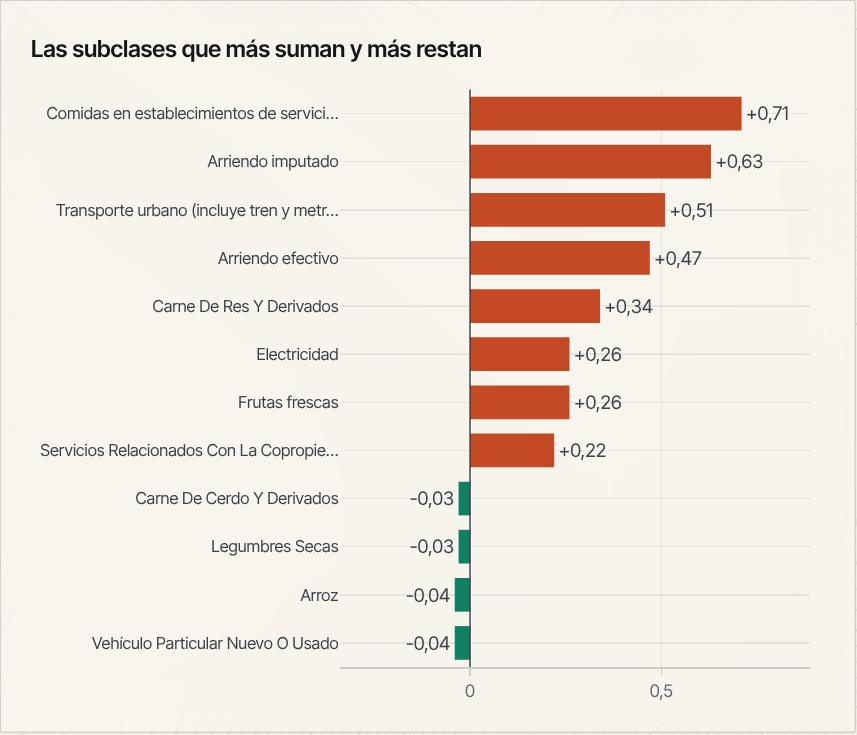
\includegraphics[width=\linewidth,height=0.42\textheight,keepaspectratio]{fig/g-inf-subclases.jpg}\end{center}
\paragraph{Qué nos cuenta}
Identifica las subclases de la canasta del IPC que más empujan la inflación anual hacia arriba y las que más la frenan. El aporte de cada subclase combina cuánto subió su precio con cuánto pesa en el gasto de los hogares, de modo que permite ver qué productos y servicios concretos explican la inflación del último mes publicado.

\begin{leer}[Cómo se lee]
Barras horizontales con el aporte de cada subclase a la inflación anual total, en puntos porcentuales (pp), con su valor rotulado: las 8 que más suman y las 4 de menor aporte (las que más restan), ordenadas de menor a mayor. Las barras naranjas suman a la inflación y las verdes restan; la línea vertical marca el cero. Al pasar el cursor se ve la inflación anual de la subclase. Los nombres largos se recortan.
\end{leer}

\paragraph{Por qué importa}
Unas pocas subclases de gran peso, como el arriendo, la electricidad, las comidas fuera del hogar o el transporte urbano, pueden explicar buena parte de la inflación. Conocerlas permite distinguir si la presión viene de bienes con precios volátiles o de servicios indexados, e identificar qué rubros pesan hoy en los costos de hogares y empresas.

\paragraph{Cómo interpretarlo}
\begin{itemize}
\item Si las mayores barras naranjas son servicios (arriendos, restaurantes, educación), la inflación tiene un componente persistente; si son alimentos o energía, uno más volátil.
\item Una subclase puede aportar mucho con una inflación moderada si su peso es grande; el recuadro flotante muestra su inflación para distinguir ambos efectos.
\item Las barras verdes señalan precios que bajaron en el año y contienen la inflación; si hay menos de cuatro subclases con aporte negativo, alguna barra del grupo inferior puede ser positiva (y se ve naranja).
\item Los aportes los calcula el DANE con ponderaciones de la canasta base 2018; la suma de las 188 subclases da la inflación total.
\end{itemize}
\begin{formulas}[Fórmulas]
\formula{Aporte de la subclase s}{A\textsubscript{s,t} = w\textsubscript{s} $\times$ (I\textsubscript{s,t−12} $\div$ I\textsubscript{t−12}) $\times$ $\pi$\textsubscript{s,t}}{w\textsubscript{s} = ponderación base 2018; I\textsubscript{s} = índice de la subclase; I = IPC total; $\pi$\textsubscript{s,t} = inflación anual de la subclase (\%)}
\formula{Suma de aportes}{$\Sigma$\textsubscript{s=1..188} A\textsubscript{s,t} = $\pi$\textsubscript{t}}{$\pi$\textsubscript{t} = inflación anual total; en pp}
\end{formulas}
\begin{metodo}[Metodología]
Contribución de cada subclase a la variación anual del IPC total (DANE), en puntos porcentuales.
\par\smallskip{\small\textbf{Fuente:} DANE, IPC base diciembre 2018 (anexos mensuales)}
\end{metodo}

\section{¿Quién siente más la inflación?}

\subsection{Inflación anual por nivel de ingreso del hogar}
\label{g:g-inf-ingresos}
\begin{center}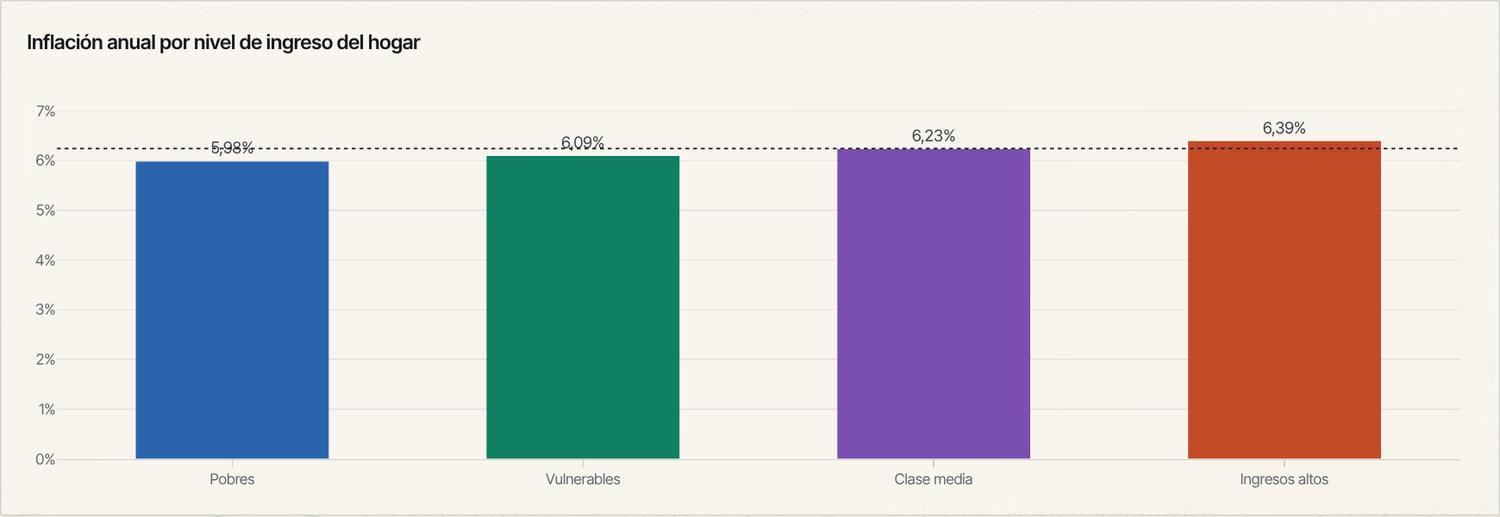
\includegraphics[width=\linewidth,height=0.42\textheight,keepaspectratio]{fig/g-inf-ingresos.jpg}\end{center}
\paragraph{Qué nos cuenta}
Compara la inflación anual que enfrentan cuatro grupos de hogares según su nivel de ingreso: pobres, vulnerables, clase media e ingresos altos. El DANE calcula un IPC para cada grupo con su propia canasta, porque los hogares de menores ingresos destinan más a alimentos y los de mayores ingresos más a servicios, de modo que un mismo cambio de precios los afecta de forma distinta.

\begin{leer}[Cómo se lee]
Eje horizontal: grupo de ingreso; eje vertical: inflación anual en \%. Cuatro barras con su valor rotulado: azul para hogares pobres, verde para vulnerables, morada para clase media y naranja para ingresos altos. La línea horizontal negra punteada es la inflación total nacional. Corresponde al último mes publicado; los grupos se definen con un criterio absoluto de ingreso basado en las líneas de pobreza.
\end{leer}

\paragraph{Por qué importa}
La inflación es un impuesto regresivo cuando golpea más a los hogares pobres, que tienen menos margen para sustituir consumo o protegerse. La diferencia entre grupos tiene implicaciones para el consumo agregado, la pobreza monetaria, el ajuste del salario mínimo y las transferencias, y ayuda a entender la composición de la inflación: si los pobres enfrentan más inflación, suelen pesar los alimentos; si los de ingresos altos, los servicios.

\paragraph{Cómo interpretarlo}
\begin{itemize}
\item Barra azul por encima de la naranja: la inflación golpea más a los hogares pobres, normalmente por alimentos; al revés, la presión está en servicios con más peso en canastas de ingresos altos.
\item Barras cerca de la línea punteada: la inflación afecta de forma similar a todos los grupos.
\item Las diferencias entre grupos suelen ser de décimas de punto porcentual, pero acumuladas por varios años cambian el costo de vida relativo.
\item Cada IPC usa las ponderaciones de gasto del grupo según la encuesta de presupuestos de los hogares de la base 2018; los precios son los mismos para todos.
\end{itemize}
\begin{formulas}[Fórmulas]
\formula{IPC del grupo h}{IPC\textsubscript{h,t} = $\Sigma$\textsubscript{s} w\textsubscript{s}\textsuperscript{h} $\times$ I\textsubscript{s,t}}{w\textsuperscript{h}\textsubscript{s} = peso de la subclase s en la canasta del grupo h ($\Sigma$ w = 1); I\textsubscript{s,t} = índice de la subclase}
\formula{Inflación anual del grupo}{$\pi$\textsubscript{h,t} = (IPC\textsubscript{h,t} $\div$ IPC\textsubscript{h,t−12} − 1) $\times$ 100}{h = pobres, vulnerables, clase media o ingresos altos}
\end{formulas}
\begin{metodo}[Metodología]
IPC calculado con la canasta de cada nivel de ingreso definido por el DANE (pobres, vulnerables, clase media e ingresos altos, según la línea de pobreza).
\par\smallskip{\small\textbf{Fuente:} DANE, IPC base diciembre 2018 (anexos mensuales)}
\end{metodo}

\section{Inflación en 23 ciudades}

\subsection{Inflación anual por ciudad (ago 2026)}
\label{g:g-inf-ciudades}
\begin{center}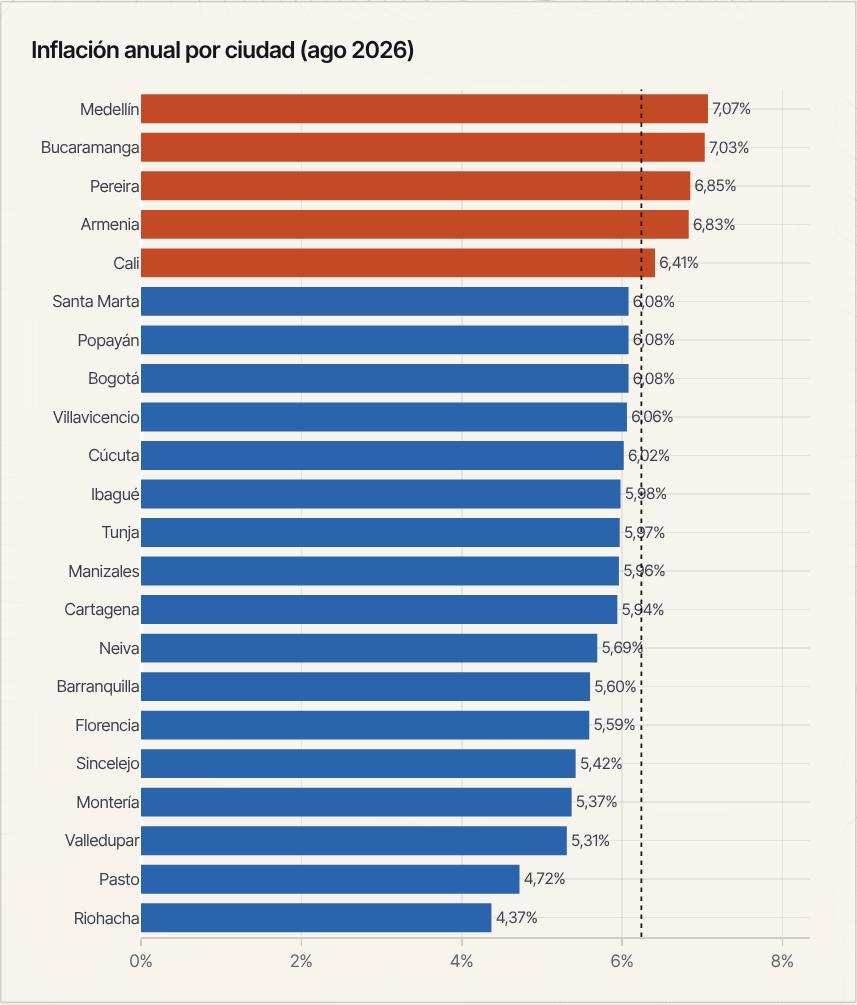
\includegraphics[width=\linewidth,height=0.42\textheight,keepaspectratio]{fig/g-inf-ciudades.jpg}\end{center}
\paragraph{Qué nos cuenta}
Compara la inflación anual del IPC total en las 23 ciudades que el DANE publica por separado, cada una con su propia canasta. Muestra qué tan homogénea es la inflación en el territorio: las diferencias reflejan la composición del gasto local, la dependencia de alimentos de distintas zonas productoras, las tarifas de servicios públicos de cada región y las condiciones de demanda locales.

\begin{leer}[Cómo se lee]
Barras horizontales ordenadas de menor a mayor inflación (la mayor arriba), en \% anual, con el valor rotulado. Las barras naranjas son ciudades con inflación por encima del total nacional y las azules, en o por debajo de él. La línea vertical negra punteada es la inflación total nacional. No se incluye el agregado de «otras áreas urbanas». Corresponde al último mes publicado.
\end{leer}

\paragraph{Por qué importa}
Para empresas con operaciones regionales, la inflación local determina costos, salarios y precios de venta en cada mercado; para inversionistas en finca raíz o consumo, revela diferencias en el poder adquisitivo regional. Las ciudades grandes, en especial Bogotá, Medellín y Cali, pesan mucho más en el total nacional, que por eso se parece más a ellas.

\paragraph{Cómo interpretarlo}
\begin{itemize}
\item El número de barras naranjas no tiene por qué ser la mitad: el total nacional es un promedio ponderado por el gasto, dominado por las ciudades grandes.
\item Las diferencias grandes entre ciudades suelen venir de tarifas de energía (muy distintas por región) y de choques de alimentos en zonas específicas.
\item El detalle por división de gasto de cada ciudad está en el mapa de calor «¿Qué sube más en cada ciudad?».
\item Las canastas de ciudades pequeñas tienen menos observaciones de precios y pueden ser más volátiles mes a mes.
\end{itemize}
\begin{formulas}[Fórmulas]
\formula{Inflación anual de la ciudad}{$\pi$\textsubscript{c,t} = (IPC\textsubscript{c,t} $\div$ IPC\textsubscript{c,t−12} − 1) $\times$ 100}{IPC\textsubscript{c,t} = índice de precios al consumidor de la ciudad c en el mes t}
\formula{Total nacional}{IPC\textsubscript{t} = $\Sigma$\textsubscript{c} $\omega$\textsubscript{c} $\times$ IPC\textsubscript{c,t}}{$\omega$\textsubscript{c} = peso de la ciudad según el gasto de sus hogares (incluye otras áreas urbanas)}
\end{formulas}
\begin{metodo}[Metodología]
Variación anual del IPC total en las 23 ciudades capitales con canasta propia.
\par\smallskip{\small\textbf{Fuente:} DANE, IPC base diciembre 2018 (anexos mensuales)}
\end{metodo}

\subsection{¿Qué sube más en cada ciudad?}
\label{g:g-inf-ciudad-division}
\begin{center}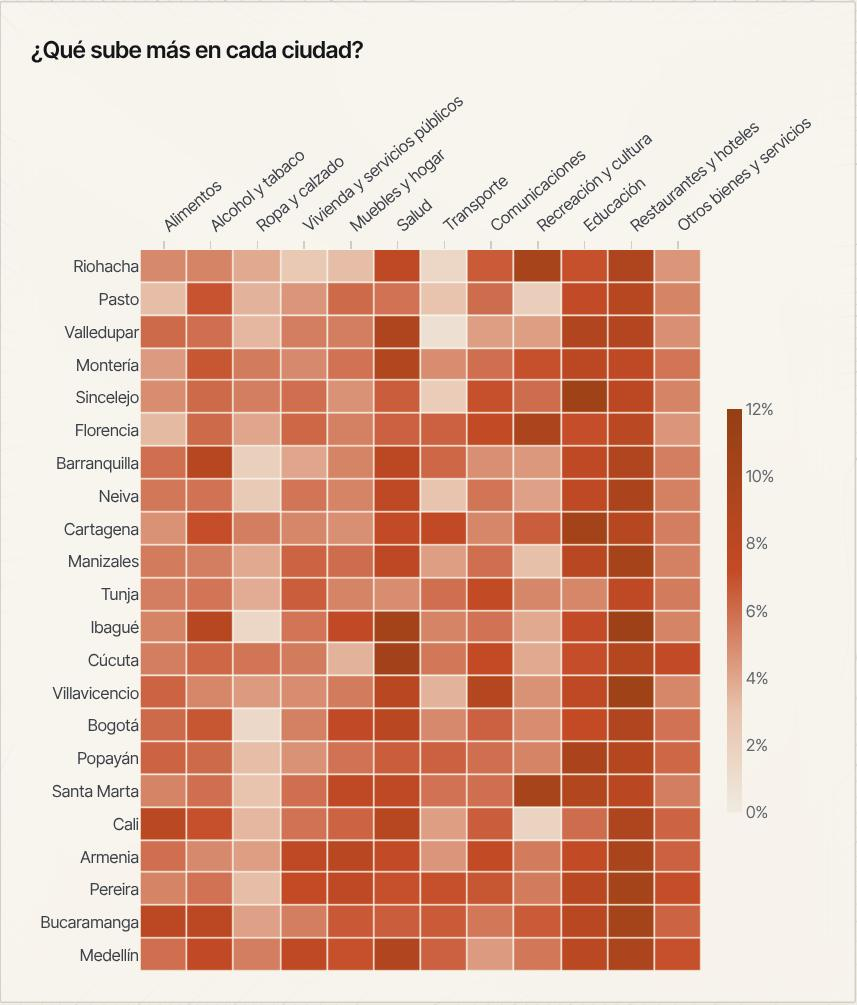
\includegraphics[width=\linewidth,height=0.42\textheight,keepaspectratio]{fig/g-inf-ciudad-division.jpg}\end{center}
\paragraph{Qué nos cuenta}
Cruza las 23 ciudades del IPC con las 12 divisiones de gasto para mostrar qué rubros suben más en cada lugar. Permite ver si la inflación de una ciudad se explica por un rubro particular, como vivienda y servicios públicos o alimentos, o si el alza es amplia, y comparar el mismo rubro entre regiones.

\begin{leer}[Cómo se lee]
Mapa de calor: cada fila es una ciudad y cada columna una división de gasto (nombres arriba). El color de cada casilla indica la inflación anual de esa división en esa ciudad: casi blanco cerca de 0\%, naranja intermedio alrededor de 7\% y naranja oscuro desde 12\%; la barra de color a la derecha da la escala. Los valores por debajo de 0\% se ven como 0\% y los superiores a 12\%, con el tono más oscuro; el recuadro flotante muestra el valor exacto. Las filas siguen el orden de la inflación total de cada ciudad. Corresponde al último mes publicado.
\end{leer}

\paragraph{Por qué importa}
Las diferencias regionales de inflación suelen concentrarse en pocos rubros: tarifas de energía que dependen del operador regional, arriendos en ciudades con alta demanda de vivienda o alimentos según la cercanía a zonas productoras. Para empresas y para el análisis de política, este cruce indica si un choque es local o nacional y en qué rubros se concentra.

\paragraph{Cómo interpretarlo}
\begin{itemize}
\item Una columna oscura en casi todas las filas indica un choque nacional en esa división; una casilla oscura aislada, un choque local.
\item Una fila mayoritariamente oscura señala una ciudad con inflación amplia, no explicada por un solo rubro.
\item La escala se recorta entre 0\% y 12\% para que los valores extremos no borren las diferencias; use el recuadro flotante para valores negativos o muy altos.
\item Las divisiones con poco peso local pueden mostrar variaciones grandes con pocas observaciones de precios; contraste con el aporte de cada división en el total nacional.
\end{itemize}
\begin{formulas}[Fórmulas]
\formula{Inflación anual por ciudad y división}{$\pi$\textsubscript{c,i,t} = (I\textsubscript{c,i,t} $\div$ I\textsubscript{c,i,t−12} − 1) $\times$ 100}{I\textsubscript{c,i,t} = índice de la división i en la ciudad c en el mes t (cuadro 6 del anexo del DANE)}
\formula{Escala de color}{z = min(max($\pi$\textsubscript{c,i,t}, 0), 12)}{valor usado para el color; el recuadro flotante muestra $\pi$ sin recortar}
\end{formulas}
\begin{metodo}[Metodología]
Variación anual por ciudad y división de gasto (cuadro 6 del anexo).
\par\smallskip{\small\textbf{Fuente:} DANE, IPC base diciembre 2018 (anexos mensuales)}
\end{metodo}

\section*{Lecturas de la página}
\begin{itemize}\small
\item \textbf{Bryan, M. F. y Cecchetti, S. G. (1994). Measuring Core Inflation. En N. G. Mankiw (ed.), Monetary Policy, 195–215. University of Chicago Press (NBER).} Medidas de inflación de fondo que excluyen los precios más volátiles.
\item \textbf{Baumol, W. J. (1967). Macroeconomics of Unbalanced Growth: The Anatomy of Urban Crisis. American Economic Review, 57(3), 415–426.} Por qué los servicios tienden a encarecerse más que los bienes.
\item \textbf{Cecchetti, S. G. (1997). Measuring Short-Run Inflation for Central Bankers. Federal Reserve Bank of St. Louis Review, 79(3), 143–155.} Dispersión y difusión de los cambios de precios.
\item \textbf{Jaravel, X. (2021). Inflation Inequality: Measurement, Causes, and Policy Implications. Annual Review of Economics, 13, 599–629.} Inflación distinta según el nivel de ingreso de los hogares.
\item \textbf{DANE. Índice de Precios al Consumidor, base diciembre 2018: metodología y canasta (2019).} Divisiones COICOP, ponderaciones, subclases, ciudades y niveles de ingreso.
\end{itemize}

\chapter{Tasas}
\label{atlas:tasas}

{\large\sffamily\bfseries Tasas de interés\par}\medskip

La tasa del Banco de la República y la tasa real: cuánto cuesta de verdad endeudarse.

{\small\color{cmmuted}Página del sitio: \url{https://stv-quant.github.io/ColombiaMacro-USBCali/tasas/}}

\section{¿Qué está haciendo el Banco de la República?}

\subsection{Tasa del Banco frente a la inflación}
\label{g:g-politica}
\begin{center}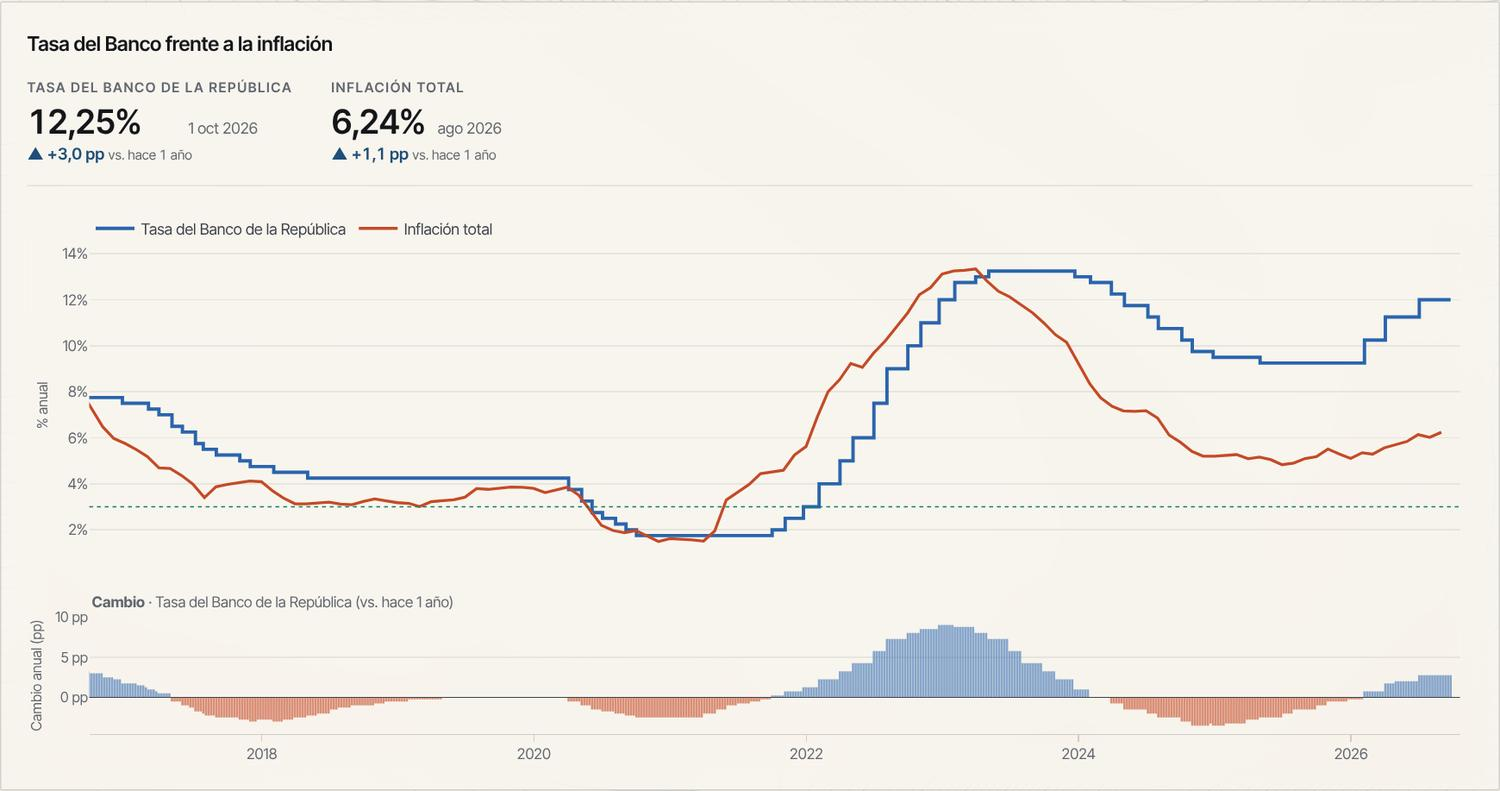
\includegraphics[width=\linewidth,height=0.42\textheight,keepaspectratio]{fig/g-politica.jpg}\end{center}
\paragraph{Qué nos cuenta}
Compara la tasa de política monetaria (TPM), la tasa de interés de intervención que fija la Junta Directiva del Banco de la República, con la inflación anual medida por el índice de precios al consumidor (IPC) del DANE. Resume la estrategia del Banco: sube la tasa cuando la inflación se aleja de la meta y la baja cuando cede. La distancia entre ambas líneas da una idea de cuán restrictiva es la política.

\begin{leer}[Cómo se lee]
Panel superior, en \% anual: la línea azul en escalones es la TPM (último dato de cada semana; cada escalón es una decisión de la Junta); la línea naranja es la inflación anual del IPC, mensual; la línea verde punteada marca la meta de inflación del 3\%. Si hay una decisión ya anunciada que aún no rige, aparece como una estrella azul en la fecha en que entra en vigor. Panel inferior: cambio de la TPM frente a un año antes, en pp (azul = subió, naranja = bajó). Vista inicial de diez años.
\end{leer}

\paragraph{Por qué importa}
La TPM es el ancla de todas las tasas de interés en pesos: del mercado interbancario, de los CDT, del crédito y de los TES. Determina el costo de financiación de empresas, hogares y Gobierno, y afecta el atractivo de los activos en pesos frente a los de otros países. Para un inversionista es la variable que más mueve la curva de rendimientos y el tipo de cambio en el corto plazo.

\paragraph{Cómo interpretarlo}
\begin{itemize}
\item Una TPM muy por encima de la inflación indica una política restrictiva (el dinero es caro en términos reales); por debajo, una política expansiva.
\item La política monetaria actúa con rezago: sus efectos sobre la inflación suelen tardar entre 12 y 24 meses, por lo que la Junta reacciona a la inflación esperada más que a la observada.
\item Una comparación más precisa es con la inflación esperada (gráfico de tasa real frente a la tasa neutral), porque la inflación observada mira hacia atrás.
\item Barras azules seguidas en el panel inferior marcan ciclos de subidas; naranjas, ciclos de bajadas (véase el gráfico de ciclos).
\end{itemize}
\begin{formulas}[Fórmulas]
\formula{Inflación anual}{$\pi$\textsubscript{t} = (IPC\textsubscript{t} $\div$ IPC\textsubscript{t−12} − 1) $\times$ 100}{IPC = índice de precios al consumidor del mes t}
\formula{Cambio anual de la TPM (panel inferior)}{$\Delta$TPM\textsubscript{t} = TPM\textsubscript{t} − TPM\textsubscript{t−1 año}}{en puntos porcentuales; TPM semanal (último dato de la semana)}
\end{formulas}
\begin{metodo}[Metodología]
Tasa de interés de intervención fijada por la Junta Directiva (escalones en cada decisión) frente a la inflación anual.
\par\smallskip{\small\textbf{Fuente:} Banco de la República, tasa de política monetaria; DANE, IPC}
\end{metodo}

\subsection{Tasa real frente a la tasa neutral}
\label{g:g-real}
\begin{center}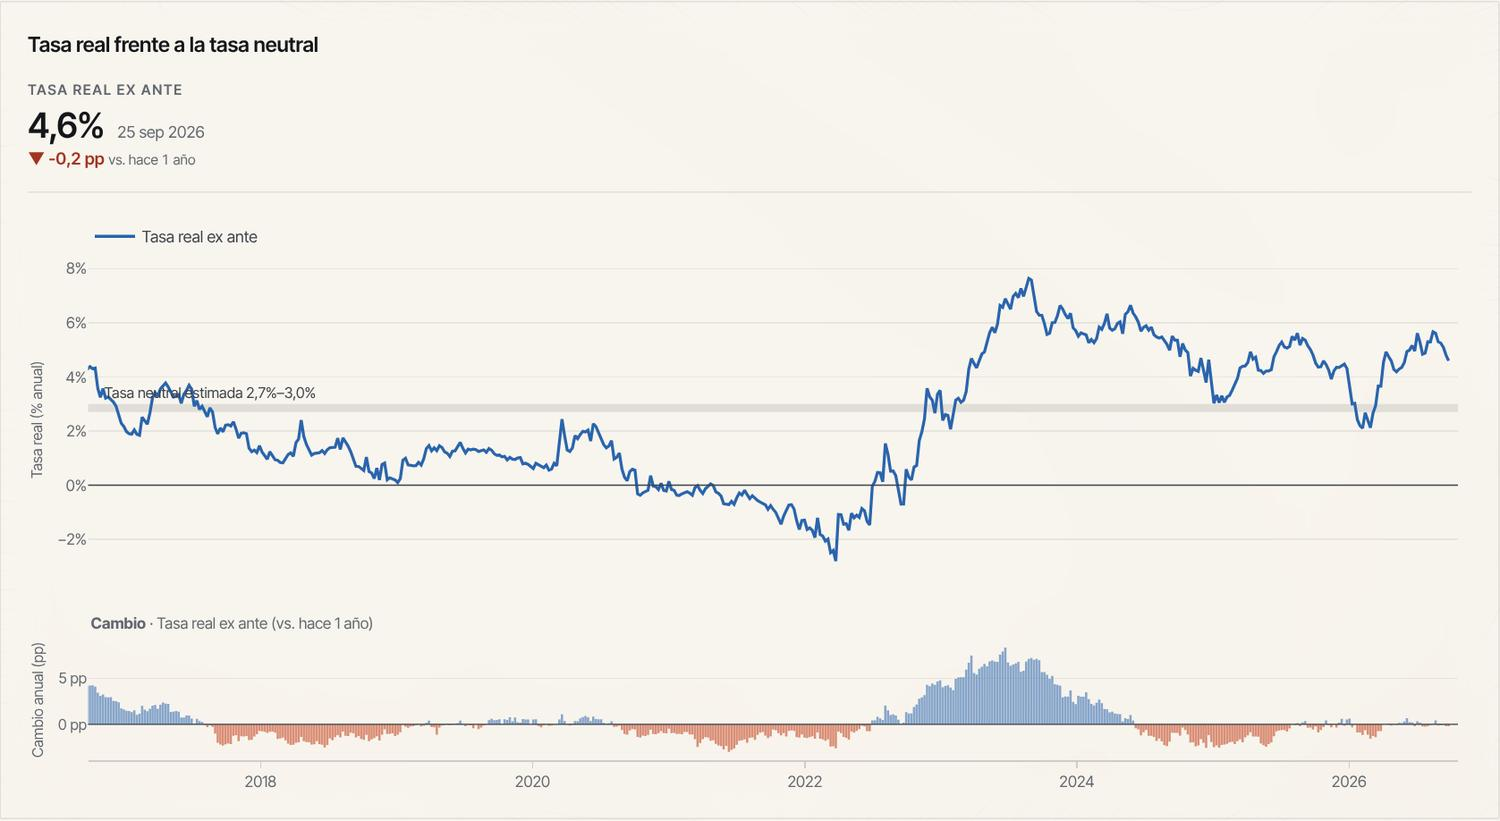
\includegraphics[width=\linewidth,height=0.42\textheight,keepaspectratio]{fig/g-real.jpg}\end{center}
\paragraph{Qué nos cuenta}
Muestra la tasa de interés real ex ante: la tasa del Banco de la República descontada la inflación que el mercado espera para los próximos 12 meses. Es lo que de verdad cuesta endeudarse en términos de poder de compra. Se compara con la tasa real neutral, el nivel que ni estimula ni frena la economía, para medir la postura de la política monetaria.

\begin{leer}[Cómo se lee]
Panel superior, en \% anual: la línea azul es la tasa real ex ante (dato semanal); la franja gris es el rango de tasa neutral estimado por el equipo técnico del Banco (2,7\%–3,0\%); la línea horizontal oscura marca el cero. La inflación esperada a un año es la inflación implícita (breakeven) en los TES (títulos de deuda pública): la diferencia entre el rendimiento a un año de los TES en pesos y el de los TES en UVR (unidad indexada a la inflación). Panel inferior: cambio frente a un año antes, en pp.
\end{leer}

\paragraph{Por qué importa}
La tasa nominal por sí sola no dice si la política es restrictiva: un 9\% con inflación esperada del 8\% es laxo, y con 3\% es muy restrictivo. La distancia frente a la neutral es la medida estándar de cuánto está frenando o estimulando el Banco la demanda. Para un inversionista determina el rendimiento real de los activos en pesos y ayuda a leer la fase del ciclo monetario.

\paragraph{Cómo interpretarlo}
\begin{itemize}
\item Por encima de la franja gris, la política frena la economía (restrictiva); dentro, es neutral; por debajo, la estimula (expansiva).
\item Una tasa real negativa (bajo la línea de cero) significa que endeudarse cuesta menos que la inflación esperada.
\item La tasa real puede subir sin que el Banco mueva su tasa, si cae la inflación esperada.
\item La inflación implícita incluye primas de riesgo y de liquidez, y la tasa neutral no es observable sino estimada con incertidumbre: lea la franja como una zona, no como un valor exacto.
\end{itemize}
\begin{formulas}[Fórmulas]
\formula{Tasa real ex ante (Fisher)}{r\textsubscript{t} = [(1 + i\textsubscript{t} $\div$ 100) $\div$ (1 + $\pi$\textsuperscript{e}\textsubscript{t} $\div$ 100) − 1] $\times$ 100}{i = tasa de política; $\pi$\textsuperscript{e} = inflación esperada a 1 año}
\formula{Inflación implícita a 1 año}{$\pi$\textsuperscript{e}\textsubscript{t} = [(1 + y\textsuperscript{pesos}\textsubscript{1a} $\div$ 100) $\div$ (1 + y\textsuperscript{UVR}\textsubscript{1a} $\div$ 100) − 1] $\times$ 100}{y = rendimiento de los TES a 1 año en pesos y en UVR}
\formula{Cambio anual (panel inferior)}{$\Delta$r\textsubscript{t} = r\textsubscript{t} − r\textsubscript{t−1 año}}{en puntos porcentuales}
\end{formulas}
\begin{metodo}[Metodología]
Tasa real ex ante = (1 + tasa del Banco) / (1 + inflación esperada a 1 año) − 1 (ecuación de Fisher). Neutral estimada por el equipo técnico del Banco: 2,7\%–3,0\%.
\par\smallskip{\small\textbf{Fuente:} Banco de la República: tasa de política y curvas TES; cálculo propio}
\end{metodo}

\section{Los ciclos de la tasa del Banco}

\subsection{Tasa del Banco y sus ciclos desde 2000}
\label{g:g-ts-ciclos}
\begin{center}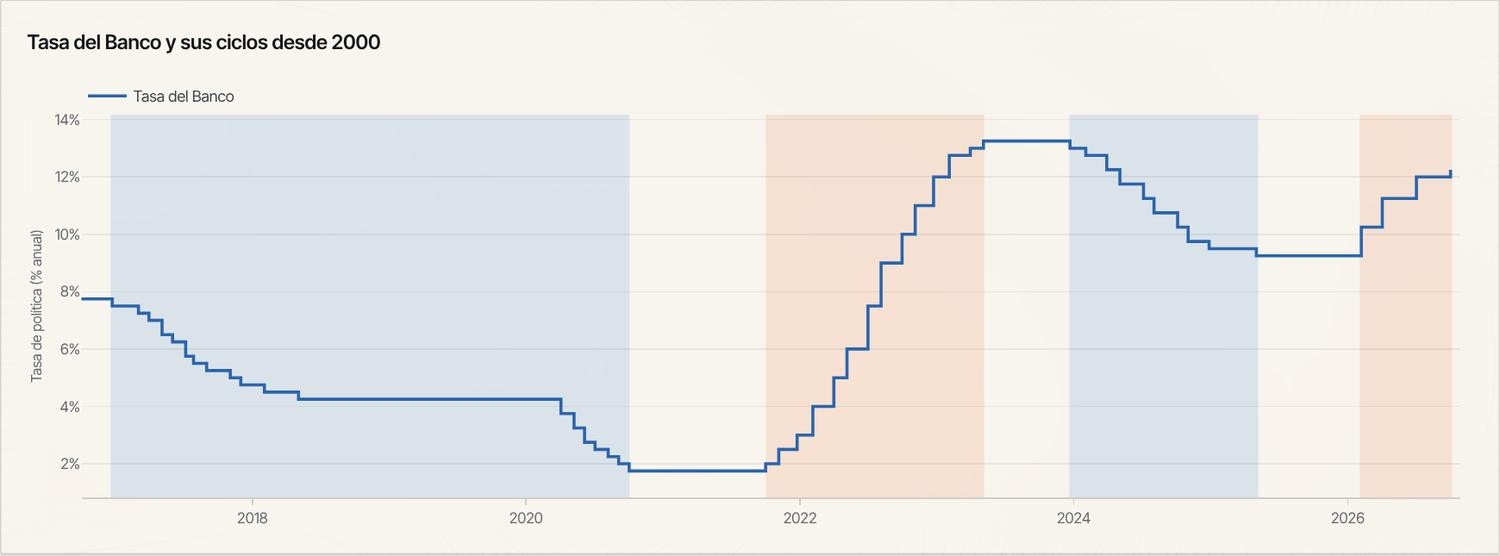
\includegraphics[width=\linewidth,height=0.42\textheight,keepaspectratio]{fig/g-ts-ciclos.jpg}\end{center}
\paragraph{Qué nos cuenta}
Muestra la trayectoria de la tasa de política monetaria (TPM) del Banco de la República desde 2000 y marca sus ciclos: periodos de subidas consecutivas para contener la inflación y periodos de bajadas consecutivas para apoyar la actividad. Permite comparar la duración y la intensidad de cada ciclo con los anteriores.

\begin{leer}[Cómo se lee]
Eje vertical en \% anual. La línea azul en escalones es la TPM (último dato de cada semana); cada escalón es una decisión de la Junta Directiva. Las franjas naranjas sombrean los ciclos de subidas y las azules los de bajadas, desde la primera hasta la última decisión en la misma dirección. Un ciclo termina cuando una decisión va en sentido contrario; las pausas (decisiones sin cambio) no lo cortan. La tabla inferior detalla cada ciclo: fechas, número de decisiones, tasa inicial y final, cambio acumulado y duración.
\end{leer}

\paragraph{Por qué importa}
Los ciclos monetarios marcan el ritmo de las tasas de interés, del crédito, de los TES y de la valoración de los activos en pesos. Conocer la amplitud y la duración de los ciclos pasados da contexto para dimensionar el actual sin asumir que se repetirá. Para un inversionista es la referencia histórica básica de la política monetaria colombiana.

\paragraph{Cómo interpretarlo}
\begin{itemize}
\item Franjas largas con escalones pequeños indican ajustes graduales; franjas cortas con escalones grandes, reacciones fuertes a choques (por ejemplo, la crisis financiera de 2008 o la pandemia de 2020).
\item Los espacios sin franja son periodos de tasa estable o con decisiones aisladas entre ciclos.
\item La amplitud de un ciclo depende del nivel de la inflación y de su distancia a la meta en cada época; los ciclos de comienzos de los 2000 ocurrieron con metas de inflación más altas.
\item El último ciclo aparece como «en curso» en la tabla hasta que una decisión vaya en sentido contrario.
\end{itemize}
\begin{formulas}[Fórmulas]
\formula{Decisión}{m\textsubscript{j} = TPM\textsubscript{d\textsubscript{j}} − TPM\textsubscript{d\textsubscript{j}−1} $\neq$ 0}{d\textsubscript{j} = fecha de la decisión j que cambia la tasa}
\formula{Cambio acumulado del ciclo}{C = $\Sigma$\textsubscript{j$\in$ciclo} m\textsubscript{j}}{suma de las decisiones consecutivas del mismo signo}
\end{formulas}
\begin{metodo}[Metodología]
Tasa de política monetaria diaria. Ciclo = decisiones consecutivas en la misma dirección; termina cuando la siguiente decisión va en sentido contrario (las pausas no cortan el ciclo).
\par\smallskip{\small\textbf{Fuente:} Banco de la República}
\end{metodo}

\section{¿Llega la tasa del Banco a los créditos y a los ahorros?}

\subsection{Tasa del Banco, interbancaria, ahorro y crédito}
\label{g:g-ts-transmision}
\begin{center}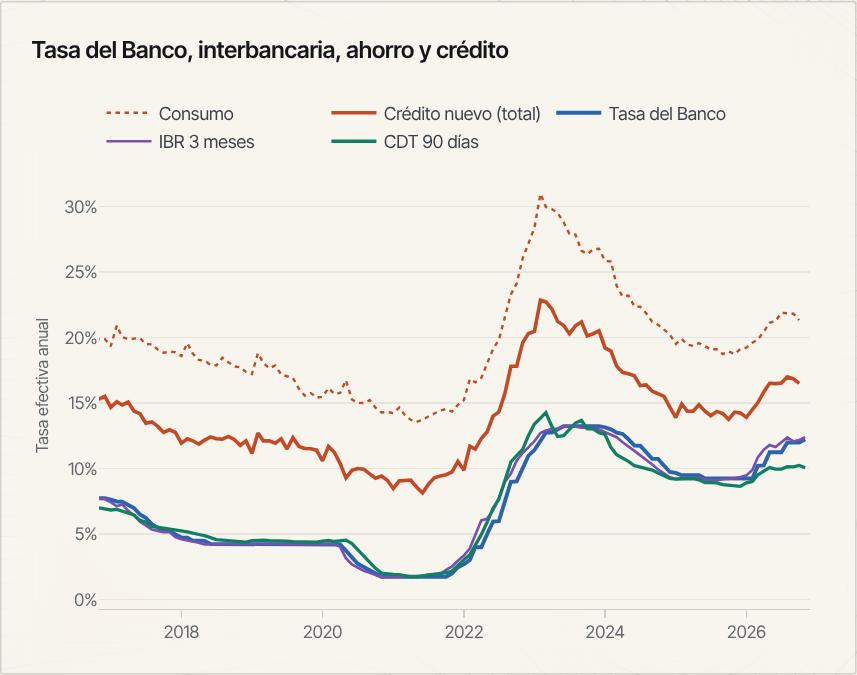
\includegraphics[width=\linewidth,height=0.42\textheight,keepaspectratio]{fig/g-ts-transmision.jpg}\end{center}
\paragraph{Qué nos cuenta}
Muestra cómo se transmite la tasa del Banco de la República a las demás tasas de la economía: el IBR a 3 meses (Indicador Bancario de Referencia, la tasa a la que los bancos se prestan pesos entre sí), los CDT a 90 días (certificados de depósito a término, lo que pagan los bancos por el ahorro) y las tasas del crédito nuevo. Permite ver si las tasas del mercado siguen a la de política, con qué rezago y con qué margen.

\begin{leer}[Cómo se lee]
Eje vertical en tasa efectiva anual, desde 2008, en promedios mensuales. Línea azul = tasa del Banco; morada = IBR a 3 meses; verde = CDT a 90 días; naranja continua = crédito nuevo total (tasa de colocación, promedio ponderado por monto desembolsado); naranja punteada = crédito de consumo. Las tasas diarias (tasa del Banco, IBR, CDT) y semanales (colocación) se promedian por mes.
\end{leer}

\paragraph{Por qué importa}
La política monetaria solo funciona si sus cambios llegan a las tasas que pagan y cobran hogares y empresas; ese es el canal de transmisión de las tasas de interés. Para un inversionista indica el costo de financiación efectivo de la economía, el rendimiento del ahorro en pesos y la rapidez con que una decisión del Banco cambia las condiciones del crédito.

\paragraph{Cómo interpretarlo}
\begin{itemize}
\item El IBR a 3 meses sigue a la tasa del Banco casi de inmediato y suele anticipar sus movimientos, porque incorpora las decisiones que el mercado descuenta para los próximos meses.
\item El CDT y el crédito reaccionan con rezago y de forma incompleta; la distancia entre crédito y CDT es el margen de los bancos (gráfico de margen).
\item El crédito de consumo está muy por encima del promedio por su mayor riesgo y costo; el crédito nuevo total incluye operaciones de tesorería de muy corto plazo y bajo riesgo, que lo acercan a las tasas de mercado.
\item Las tasas son nominales: compárelas con la inflación para ver su nivel real (gráfico de crédito por modalidad).
\end{itemize}
\begin{formulas}[Fórmulas]
\formula{Promedio mensual}{$\bar{\mathrm{R}}$\textsubscript{m} = (1 $\div$ n\textsubscript{m}) $\times$ $\Sigma$\textsubscript{d$\in$m} R\textsubscript{d}}{R = tasa diaria o semanal; n\textsubscript{m} = número de datos del mes m}
\end{formulas}
\begin{metodo}[Metodología]
Promedios mensuales de datos diarios (tasa del Banco, IBR, CDT) y semanales (colocación). Tasas efectivas anuales.
\par\smallskip{\small\textbf{Fuente:} Banco de la República con información de la Superintendencia Financiera (formato 088)}
\end{metodo}

\subsection{¿Cuánto de cada ciclo llegó a cada tasa?}
\label{g:g-ts-traspaso}
\begin{center}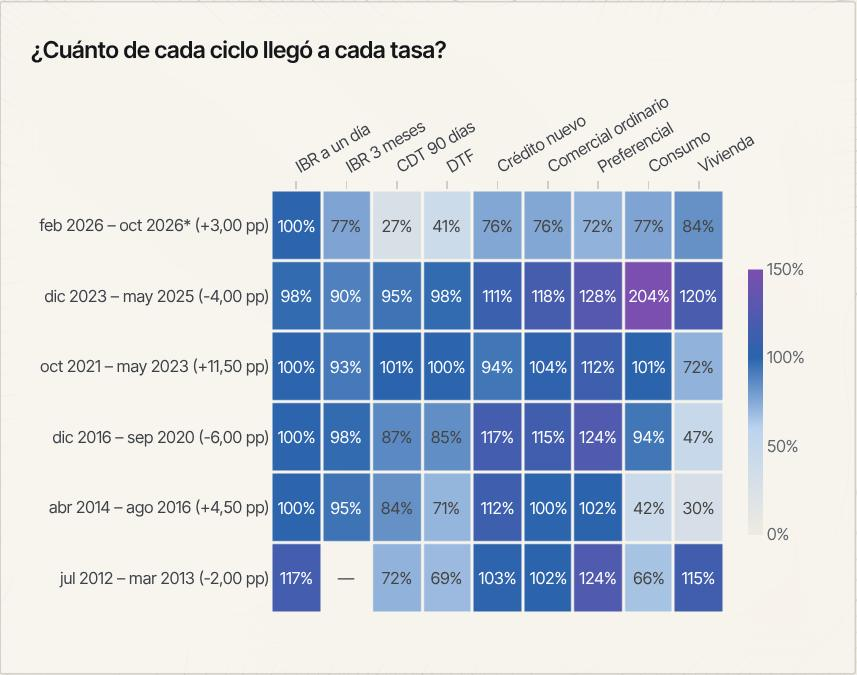
\includegraphics[width=\linewidth,height=0.42\textheight,keepaspectratio]{fig/g-ts-traspaso.jpg}\end{center}
\paragraph{Qué nos cuenta}
Mide el traspaso de cada ciclo de la tasa del Banco a nueve tasas del mercado: qué porcentaje del cambio acumulado de la tasa de política llegó a cada una. Compara los últimos ciclos desde 2008 y muestra que la transmisión es heterogénea: rápida y casi completa en el mercado interbancario, más lenta o parcial en el ahorro y en algunas modalidades de crédito.

\begin{leer}[Cómo se lee]
Mapa de calor: cada fila es un ciclo (fechas de la primera y la última decisión y, entre paréntesis, el cambio total de la tasa del Banco en pp); cada columna es una tasa: IBR a un día y a 3 meses, CDT a 90 días, DTF (promedio de captación a 90 días), crédito nuevo total, comercial ordinario, preferencial (corporativo), consumo y vivienda. El número de cada celda es el traspaso en \%; el color va de claro (0\% o menos) a azul (cerca de 100\%) y morado (150\% o más). «—» = la serie no existía al inicio del ciclo; * = ciclo en curso.
\end{leer}

\paragraph{Por qué importa}
El traspaso indica cuánto de una decisión del Banco termina en el costo del crédito y en el rendimiento del ahorro, y por tanto la potencia de la política monetaria. Para un inversionista ayuda a entender cuánto se mueven el costo de financiación, los márgenes bancarios y las tasas de los depósitos ante un ciclo de política.

\paragraph{Cómo interpretarlo}
\begin{itemize}
\item 100\% = la tasa se movió lo mismo que la del Banco; menos de 100\% = traspaso parcial; más de 100\% = se movió más (por ejemplo, por cambios en las primas de riesgo).
\item Un traspaso bajo en el CDT con uno alto en el crédito amplía el margen de los bancos, y al revés.
\item La ventana va desde el día antes de la primera decisión hasta tres meses después de la última; en el ciclo en curso se mide hasta el último dato, por lo que el traspaso puede estar incompleto.
\item El traspaso no aísla la política monetaria: en la misma ventana influyen el riesgo de crédito, la liquidez y otros choques. Valores negativos aparecen con el color más claro.
\end{itemize}
\begin{formulas}[Fórmulas]
\formula{Traspaso}{P\textsubscript{k} = (R\textsubscript{k,t1} − R\textsubscript{k,t0}) $\div$ (TPM\textsubscript{t1} − TPM\textsubscript{t0}) $\times$ 100}{R\textsubscript{k} = tasa k; t0 = día anterior a la primera decisión del ciclo; t1 = tres meses después de la última decisión (o último dato)}
\end{formulas}
\begin{metodo}[Metodología]
Traspaso = (tasa en t1 − tasa en t0) / (tasa del Banco en t1 − tasa del Banco en t0) $\times$ 100, con t0 = día anterior a la primera decisión del ciclo y t1 = tres meses después de la última (o el último dato). Ciclos desde 2008; «—» = la serie aún no existía.
\par\smallskip{\small\textbf{Fuente:} Banco de la República con información de la Superintendencia Financiera (formato 088)}
\end{metodo}

\section{¿Cuánto cuesta el crédito?}

\subsection{Tasa del crédito nuevo por modalidad}
\label{g:g-ts-modalidades}
\begin{center}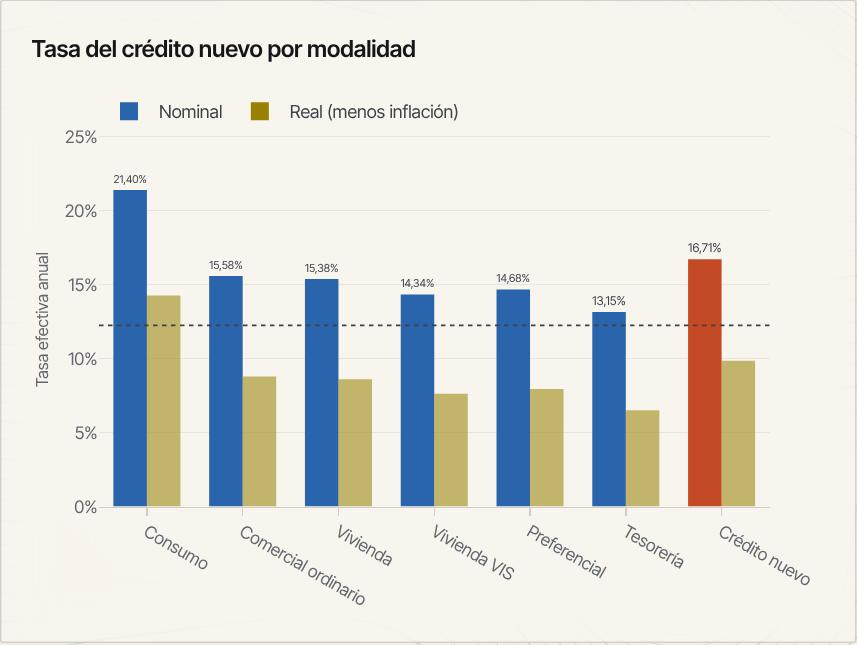
\includegraphics[width=\linewidth,height=0.42\textheight,keepaspectratio]{fig/g-ts-modalidades.jpg}\end{center}
\paragraph{Qué nos cuenta}
Compara cuánto cuesta hoy el crédito nuevo en pesos según su modalidad: consumo, comercial ordinario, vivienda (no VIS y VIS, la vivienda de interés social), preferencial o corporativo, tesorería y el promedio total. Muestra cada tasa en términos nominales y reales, y frente a la tasa del Banco de la República.

\begin{leer}[Cómo se lee]
Eje vertical en tasa efectiva anual. Para cada modalidad hay dos barras: la de color sólido es la tasa nominal del último dato semanal (azul; el promedio total en naranja) y la ámbar clara es la tasa real, descontada la inflación anual del IPC más reciente. La línea horizontal punteada es la tasa del Banco vigente. Las tasas son promedios ponderados por monto desembolsado, informados por los bancos a la Superintendencia Financiera (formato 088).
\end{leer}

\paragraph{Por qué importa}
El costo del crédito determina la inversión de las empresas, la compra de vivienda y el consumo financiado de los hogares. La diferencia entre modalidades refleja el riesgo, el plazo, las garantías y el costo de originar cada tipo de préstamo. Para un inversionista indica las condiciones financieras que enfrentan los distintos sectores y la rentabilidad potencial de cada segmento de la banca.

\paragraph{Cómo interpretarlo}
\begin{itemize}
\item La distancia entre cada barra nominal y la línea punteada es la prima que cobran los bancos sobre la tasa del Banco en esa modalidad.
\item Una tasa real alta indica condiciones financieras restrictivas para ese segmento; una cercana a cero o negativa, condiciones holgadas.
\item Tesorería y preferencial son préstamos a grandes empresas, de corto plazo y bajo riesgo, por eso quedan cerca de la tasa del Banco; consumo es el más caro.
\item La tasa real usa la inflación pasada (ex post), no la esperada, y los datos semanales son volátiles: un solo dato puede verse afectado por desembolsos puntuales.
\end{itemize}
\begin{formulas}[Fórmulas]
\formula{Tasa real de cada modalidad}{r\textsubscript{k} = [(1 + i\textsubscript{k} $\div$ 100) $\div$ (1 + $\pi$ $\div$ 100) − 1] $\times$ 100}{i\textsubscript{k} = tasa nominal efectiva anual de la modalidad k (último dato semanal); $\pi$ = inflación anual del IPC más reciente}
\end{formulas}
\begin{metodo}[Metodología]
Último dato semanal de cada modalidad. Tasa real = (1 + nominal)/(1 + inflación anual del IPC) − 1.
\par\smallskip{\small\textbf{Fuente:} Banco de la República con información de la Superintendencia Financiera (formato 088)}
\end{metodo}

\subsection{Margen de intermediación y prima del consumo}
\label{g:g-ts-margen}
\begin{center}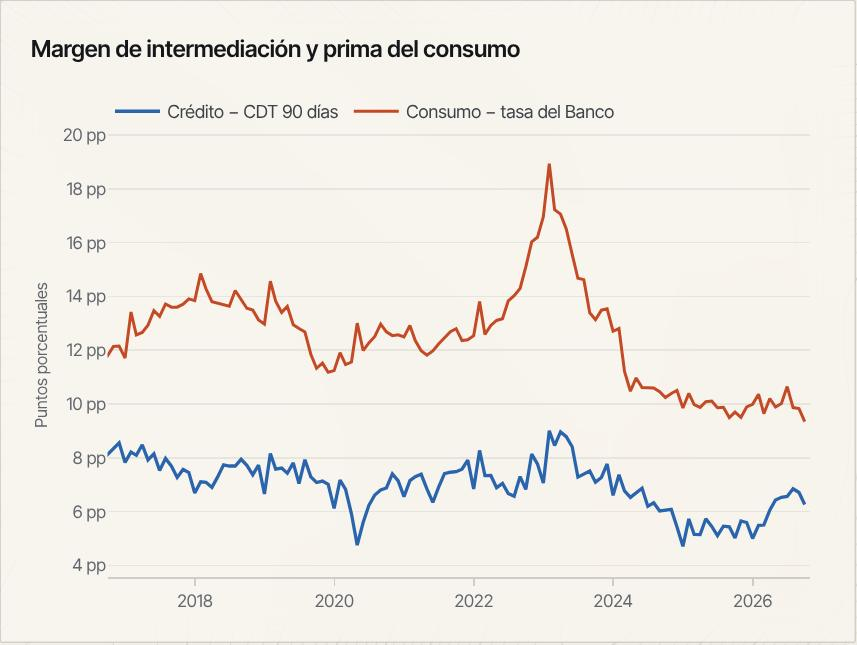
\includegraphics[width=\linewidth,height=0.42\textheight,keepaspectratio]{fig/g-ts-margen.jpg}\end{center}
\paragraph{Qué nos cuenta}
Muestra dos diferencias de tasas que resumen el negocio de los bancos y la prima de riesgo de los hogares: el margen de intermediación (tasa del crédito nuevo total menos la de los CDT a 90 días, es decir, lo que cobran los bancos por prestar frente a lo que pagan por captar) y la prima del consumo (tasa del crédito de consumo menos la tasa del Banco de la República).

\begin{leer}[Cómo se lee]
Eje vertical en puntos porcentuales (pp), desde 2008, con promedios mensuales. Línea azul = crédito nuevo total − CDT a 90 días. Línea naranja = crédito de consumo − tasa del Banco. Cada línea se calcula restando los promedios mensuales de las tasas diarias o semanales correspondientes.
\end{leer}

\paragraph{Por qué importa}
El margen de intermediación refleja el costo, el riesgo y el grado de competencia del sistema bancario, y determina cuánto del ahorro llega como crédito a un costo razonable. La prima del consumo mide cuánto más pagan los hogares que la tasa de referencia, en función del riesgo percibido. Para un inversionista son indicadores de la rentabilidad bancaria y de la percepción de riesgo de crédito.

\paragraph{Cómo interpretarlo}
\begin{itemize}
\item Un margen que se amplía puede reflejar mayor riesgo percibido, costos más altos o un traspaso más lento hacia el ahorro que hacia el crédito; uno que se estrecha, lo contrario.
\item La prima del consumo suele subir cuando aumenta la morosidad de los hogares y bajar cuando la competencia por clientes se intensifica.
\item Durante los ciclos de la tasa del Banco ambas líneas se mueven temporalmente porque las tasas no se ajustan al mismo ritmo (véase el gráfico de traspaso).
\item El crédito nuevo total mezcla modalidades; un cambio en la composición de los desembolsos puede mover el margen sin que cambie ninguna tasa.
\end{itemize}
\begin{formulas}[Fórmulas]
\formula{Margen de intermediación}{M\textsubscript{m} = $\bar{\mathrm{R}}$\textsuperscript{crédito}\textsubscript{m} − $\bar{\mathrm{R}}$\textsuperscript{CDT90}\textsubscript{m}}{$\bar{\mathrm{R}}$ = promedio mensual de la tasa; en pp}
\formula{Prima del consumo}{P\textsubscript{m} = $\bar{\mathrm{R}}$\textsuperscript{consumo}\textsubscript{m} − $\bar{\mathrm{R}}$\textsuperscript{TPM}\textsubscript{m}}{TPM = tasa de política monetaria; en pp}
\end{formulas}
\begin{metodo}[Metodología]
Diferencias de promedios mensuales: colocación total − CDT a 90 días; consumo − tasa de política.
\par\smallskip{\small\textbf{Fuente:} Banco de la República con información de la Superintendencia Financiera (formato 088)}
\end{metodo}

\section{El mercado de dinero de corto plazo}

\subsection{La curva del IBR: hoy, hace 3 meses y hace un año}
\label{g:g-ts-ibr}
\begin{center}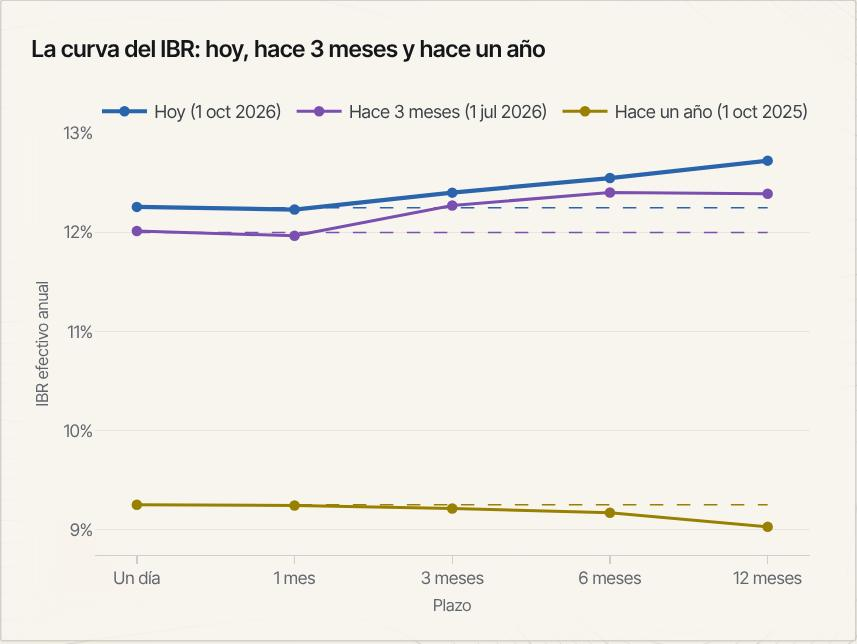
\includegraphics[width=\linewidth,height=0.42\textheight,keepaspectratio]{fig/g-ts-ibr.jpg}\end{center}
\paragraph{Qué nos cuenta}
Muestra la curva del IBR (Indicador Bancario de Referencia): las tasas a las que los bancos están dispuestos a prestarse pesos a un día, 1, 3, 6 y 12 meses. Compara la curva de hoy con la de hace 3 meses y la de hace un año, junto a la tasa del Banco de la República en cada fecha. Su forma resume cómo valora el mercado el costo del dinero en los próximos meses.

\begin{leer}[Cómo se lee]
Eje horizontal: plazo (un día, 1 mes, 3 meses, 6 meses, 12 meses). Eje vertical: IBR en tasa efectiva anual. Línea azul = hoy; morada = hace 3 meses; ámbar = hace un año (la fecha exacta aparece en la leyenda; se usa el último dato disponible en o antes de cada fecha). La raya horizontal discontinua del mismo color es la tasa del Banco vigente en esa fecha.
\end{leer}

\paragraph{Por qué importa}
El IBR es la referencia de muchos créditos a tasa variable, de los swaps de tasa de interés y de la valoración de deuda de corto plazo. La pendiente de la curva incorpora la trayectoria de la tasa del Banco que el mercado descuenta, por lo que es un termómetro diario de las condiciones del mercado monetario. Para un inversionista sirve para valorar instrumentos en pesos y medir el costo de cubrir riesgo de tasa.

\paragraph{Cómo interpretarlo}
\begin{itemize}
\item Si los plazos largos están por encima del de un día, el mercado cobra más por prestar a más tiempo, lo que es coherente con subidas de la tasa del Banco incorporadas en los precios; si están por debajo, con bajadas incorporadas.
\item El IBR a un día debe quedar pegado a la raya de la tasa del Banco; una distancia grande indicaría problemas de liquidez (véase el gráfico de tasas a un día).
\item Un desplazamiento de toda la curva entre fechas refleja decisiones ya tomadas; un cambio de pendiente, un cambio en lo que el mercado descuenta.
\item Las tasas a plazo también contienen primas por plazo y liquidez: no son una medida pura de expectativas.
\end{itemize}
\begin{formulas}[Fórmulas]
\formula{Diferencia frente a la tasa del Banco}{S\textsubscript{h} = IBR\textsubscript{h} − TPM}{h = plazo; distancia vertical entre cada punto y la raya del mismo color}
\end{formulas}
\begin{metodo}[Metodología]
IBR efectivo anual por plazo en la última fecha, hace 3 meses y hace un año (último dato disponible en o antes de cada fecha).
\par\smallskip{\small\textbf{Fuente:} Banco de la República}
\end{metodo}

\subsection{Tasas a un día frente a la tasa del Banco}
\label{g:g-ts-overnight}
\begin{center}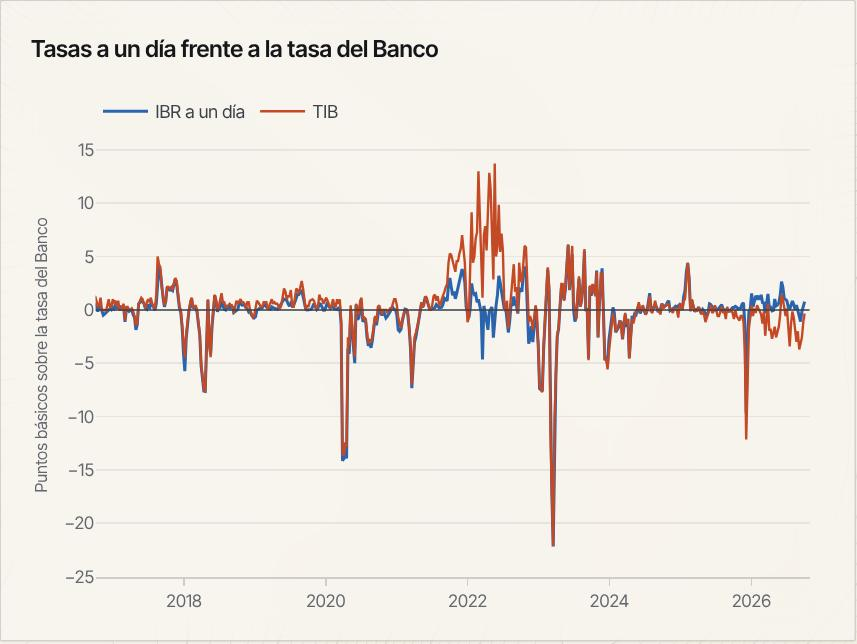
\includegraphics[width=\linewidth,height=0.42\textheight,keepaspectratio]{fig/g-ts-overnight.jpg}\end{center}
\paragraph{Qué nos cuenta}
Mide qué tan bien controla el Banco de la República el costo del dinero a un día. Compara dos tasas de muy corto plazo con la tasa de política: el IBR a un día y la TIB (tasa interbancaria, préstamos entre bancos sin garantía a un día). Si ambas se mantienen cerca de la tasa del Banco, la decisión de la Junta se cumple efectivamente en el mercado.

\begin{leer}[Cómo se lee]
Eje vertical en puntos básicos (pb; 100 pb = 1 pp) por encima o por debajo de la tasa del Banco, desde 2008. Línea azul = IBR a un día − tasa del Banco; línea naranja = TIB − tasa del Banco. Cada punto es el promedio semanal de las diferencias diarias. La línea horizontal oscura marca el cero (tasa igual a la del Banco).
\end{leer}

\paragraph{Por qué importa}
El primer eslabón de la transmisión monetaria es el mercado interbancario a un día: si allí la tasa se aparta de la de política, la señal del Banco se diluye antes de llegar al resto de tasas. Para un inversionista, desviaciones grandes o persistentes son señales de tensiones de liquidez en el sistema financiero.

\paragraph{Cómo interpretarlo}
\begin{itemize}
\item Valores cercanos a cero indican un control efectivo; desvíos de unos pocos puntos básicos son normales.
\item Picos positivos suelen coincidir con estrechez de liquidez (pagos de impuestos, cierres de mes o de año); valores negativos, con exceso de pesos en el sistema.
\item La TIB es más volátil que el IBR porque refleja operaciones efectivas entre pocos participantes, mientras el IBR se construye con cotizaciones de varios bancos.
\item Compárelo con el gráfico de liquidez: las subastas de expansión y la ventanilla de contracción son los instrumentos con que el Banco cierra estas brechas.
\end{itemize}
\begin{formulas}[Fórmulas]
\formula{Diferencia diaria}{s\textsubscript{d} = (R\textsubscript{d} − TPM\textsubscript{d}) $\times$ 100}{R = IBR a un día o TIB del día d (en \%); resultado en puntos básicos}
\formula{Promedio semanal}{S\textsubscript{w} = (1 $\div$ n\textsubscript{w}) $\times$ $\Sigma$\textsubscript{d$\in$w} s\textsubscript{d}}{n\textsubscript{w} = número de días con dato en la semana w}
\end{formulas}
\begin{metodo}[Metodología]
Promedio semanal de (IBR a un día − tasa de política) y (TIB − tasa de política), en puntos básicos.
\par\smallskip{\small\textbf{Fuente:} Banco de la República con información de la Superintendencia Financiera}
\end{metodo}

\section{¿Cuánto crédito hay y cuánto crece?}

\subsection{Crecimiento real del crédito por modalidad}
\label{g:g-ts-cartera}
\begin{center}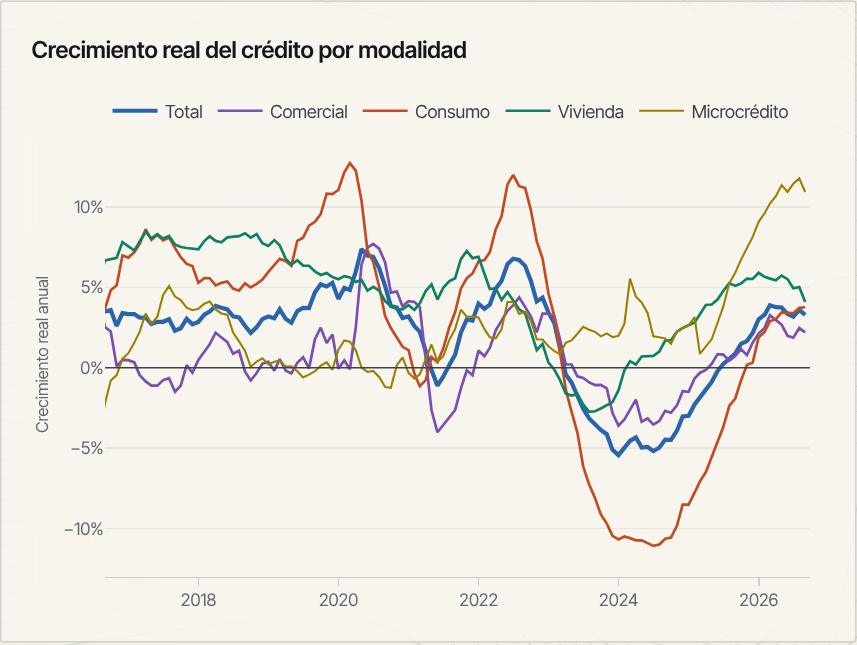
\includegraphics[width=\linewidth,height=0.42\textheight,keepaspectratio]{fig/g-ts-cartera.jpg}\end{center}
\paragraph{Qué nos cuenta}
Muestra a qué ritmo crece el saldo de crédito en pesos (la cartera de los establecimientos de crédito) una vez descontada la inflación, en total y por modalidad: comercial (empresas), consumo (hogares), vivienda y microcrédito. Indica si el sistema financiero está expandiendo o contrayendo en términos reales el financiamiento a la economía.

\begin{leer}[Cómo se lee]
Eje vertical: variación anual real, en \%, desde 2008; la línea horizontal oscura marca el cero. Línea azul gruesa = cartera total; morada = comercial; naranja = consumo; verde = vivienda; ámbar = microcrédito. Cada punto compara el saldo de fin de mes con el del mismo mes un año antes y descuenta la inflación anual del IPC de ese mes. La cartera total es la cartera bruta sin ajuste por titularización y la de vivienda es la hipotecaria ajustada por titularizaciones.
\end{leer}

\paragraph{Por qué importa}
El crédito financia la inversión de las empresas y el consumo de los hogares, por lo que su crecimiento real acompaña al ciclo económico y es un canal clave de la política monetaria. Para un inversionista indica la fase del ciclo crediticio, el dinamismo de la demanda interna y las perspectivas de ingreso de los bancos.

\paragraph{Cómo interpretarlo}
\begin{itemize}
\item Por encima de cero, el crédito crece más que los precios (expansión real); por debajo, se contrae en términos reales.
\item El crédito suele reaccionar con rezago a la tasa del Banco: tasas reales altas tienden a moderar su crecimiento después de varios trimestres.
\item El consumo suele ser la modalidad más cíclica; la vivienda, la más estable por sus plazos largos.
\item Desde 2015 la contabilidad bancaria usa NIIF, un cambio metodológico; además, las titularizaciones y castigos de cartera pueden alterar el saldo sin que cambien los desembolsos.
\end{itemize}
\begin{formulas}[Fórmulas]
\formula{Crecimiento nominal anual}{g\textsubscript{t} = C\textsubscript{t} $\div$ C\textsubscript{t−12} − 1}{C = saldo de cartera en pesos a fin del mes t}
\formula{Crecimiento real anual}{g\textsuperscript{r}\textsubscript{t} = [(1 + g\textsubscript{t}) $\div$ (1 + $\pi$\textsubscript{t} $\div$ 100) − 1] $\times$ 100}{$\pi$ = inflación anual del IPC del mes t (\%)}
\end{formulas}
\begin{metodo}[Metodología]
Crecimiento real = (1 + variación anual del saldo)/(1 + inflación anual) − 1. Cartera bruta sin ajuste por titularización; vivienda: cartera hipotecaria ajustada. Desde 2015, NIIF.
\par\smallskip{\small\textbf{Fuente:} Banco de la República (cartera en moneda legal); DANE (IPC)}
\end{metodo}

\subsection{¿Para qué se presta? Composición del crédito}
\label{g:g-ts-composicion}
\begin{center}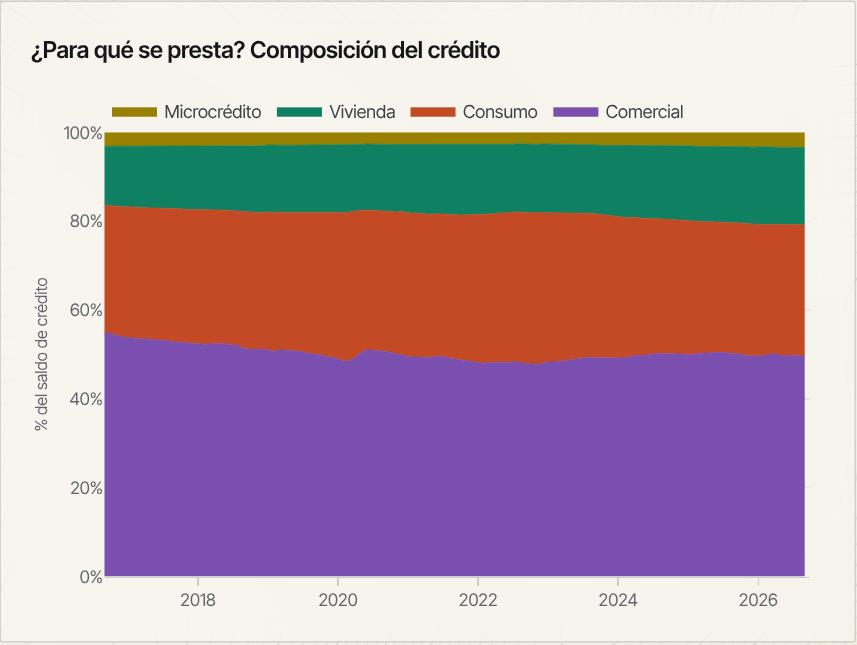
\includegraphics[width=\linewidth,height=0.42\textheight,keepaspectratio]{fig/g-ts-composicion.jpg}\end{center}
\paragraph{Qué nos cuenta}
Muestra cómo se reparte el saldo de crédito en pesos entre las cuatro modalidades: comercial (empresas), consumo (hogares, para gastos distintos de vivienda), vivienda y microcrédito (pequeños negocios). Revela hacia dónde se dirige el financiamiento bancario y cómo ha cambiado el peso relativo de empresas y hogares en el balance de los bancos.

\begin{leer}[Cómo se lee]
Áreas apiladas que suman 100\% (eje de 0\% a 100\%), desde 2008, con datos mensuales. De abajo hacia arriba: morado = comercial; naranja = consumo; verde = vivienda (cartera hipotecaria ajustada por titularizaciones); ámbar = microcrédito. El denominador es la suma de las cuatro modalidades en moneda legal, no la cartera bruta total.
\end{leer}

\paragraph{Por qué importa}
La composición del crédito influye en la sensibilidad del sistema financiero al ciclo y en el canal por el que actúa la política monetaria. Más peso del consumo hace la cartera más rentable pero también más expuesta al deterioro del empleo y del ingreso de los hogares; más peso comercial la liga a la inversión y al desempeño de las empresas. Para un inversionista es un indicador del perfil de riesgo de la banca.

\paragraph{Cómo interpretarlo}
\begin{itemize}
\item Una franja de consumo que se ensancha indica que el crédito a los hogares crece más rápido que el resto.
\item Los cambios de composición son lentos; movimientos de un punto en un año ya son relevantes.
\item Una participación puede caer porque esa cartera crece menos que las demás, no necesariamente porque se contraiga; compárelo con el crecimiento real por modalidad.
\item Titularizaciones, castigos y reclasificaciones entre modalidades pueden alterar la composición sin cambios en la actividad.
\end{itemize}
\begin{formulas}[Fórmulas]
\formula{Participación de cada modalidad}{S\textsubscript{k,t} = C\textsubscript{k,t} $\div$ (C\textsubscript{com,t} + C\textsubscript{cons,t} + C\textsubscript{viv,t} + C\textsubscript{mic,t}) $\times$ 100}{C = saldo en pesos de cada modalidad a fin del mes t}
\end{formulas}
\begin{metodo}[Metodología]
Participación de cada modalidad en la suma de comercial, consumo, vivienda (ajustada) y microcrédito en moneda legal.
\par\smallskip{\small\textbf{Fuente:} Banco de la República}
\end{metodo}

\section{La liquidez que da el Banco}

\subsection{Repos de expansión y depósitos de contracción}
\label{g:g-ts-liquidez}
\begin{center}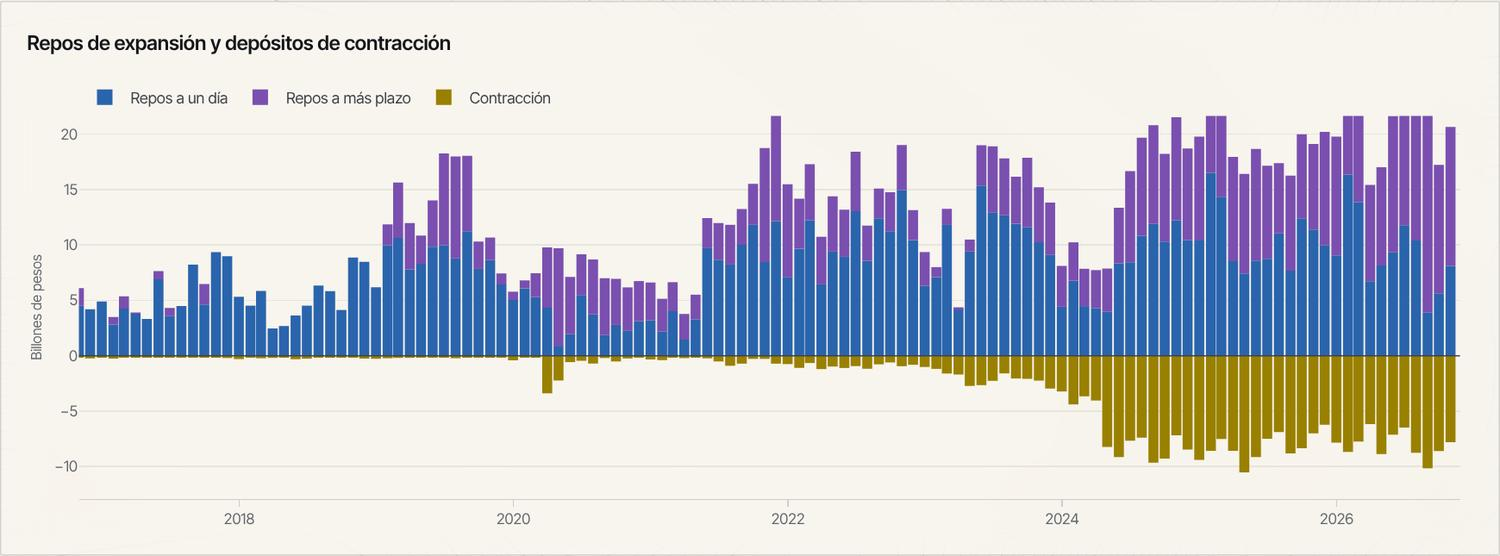
\includegraphics[width=\linewidth,height=0.42\textheight,keepaspectratio]{fig/g-ts-liquidez.jpg}\end{center}
\paragraph{Qué nos cuenta}
Muestra cómo el Banco de la República ajusta la cantidad de pesos en el sistema financiero para que la tasa a un día se mantenga cerca de la tasa de política. Arriba, los repos de expansión: préstamos de corto plazo del Banco a las entidades financieras con garantía de títulos. Abajo, la ventanilla de contracción: depósitos remunerados que las entidades hacen en el Banco con sus excedentes de liquidez.

\begin{leer}[Cómo se lee]
Barras mensuales en billones de pesos, desde 2012. Hacia arriba (valores positivos): azul = repos de expansión a un día; morado = repos a plazos mayores de un día. Hacia abajo (valores negativos): ámbar = saldo en la ventanilla de contracción. Cada barra es el promedio del mes de los saldos diarios (los días sin operación cuentan como cero). La línea horizontal marca el cero.
\end{leer}

\paragraph{Por qué importa}
Es la cara operativa de la política monetaria: la Junta fija la tasa y el Banco provee o retira liquidez para que se cumpla en el mercado. Un uso alto de los repos indica que los bancos necesitan pesos (por ejemplo, por pagos de impuestos, menor ahorro o crecimiento del crédito); depósitos de contracción altos, que les sobran. Para un inversionista es una señal de las condiciones de liquidez del mercado de dinero y de los TES de corto plazo.

\paragraph{Cómo interpretarlo}
\begin{itemize}
\item Barras azules y moradas crecientes indican una mayor necesidad de liquidez del sistema; barras ámbar más profundas, excedentes que el Banco absorbe.
\item Los saldos tienen estacionalidad: suben en fechas de pago de impuestos y en fin de año; compare con los mismos meses de años anteriores.
\item Las compras o ventas de TES y de divisas por parte del Banco también cambian la liquidez y no aparecen en este gráfico.
\item Léalo con el gráfico de tasas a un día: si la liquidez se ajusta bien, el IBR y la TIB permanecen cerca de la tasa del Banco.
\end{itemize}
\begin{formulas}[Fórmulas]
\formula{Promedio mensual de saldos}{$\bar{\mathrm{L}}$\textsubscript{k,m} = (1 $\div$ n\textsubscript{m}) $\times$ $\Sigma$\textsubscript{d$\in$m} L\textsubscript{k,d} $\div$ 1.000}{L = saldo diario del instrumento k (miles de millones de pesos; 0 si no hubo operación); n\textsubscript{m} = días del mes con registro; resultado en billones}
\formula{Posición neta (lectura)}{N\textsubscript{m} = $\bar{\mathrm{L}}$\textsubscript{repo 1 día,m} + $\bar{\mathrm{L}}$\textsubscript{repo plazo,m} − $\bar{\mathrm{L}}$\textsubscript{contracción,m}}{positivo = el Banco presta en neto al sistema}
\end{formulas}
\begin{metodo}[Metodología]
Saldos diarios de subastas de expansión a un día y a otros plazos, y de la ventanilla de contracción, promediados por mes (billones de pesos).
\par\smallskip{\small\textbf{Fuente:} Banco de la República}
\end{metodo}

\section*{Lecturas de la página}
\begin{itemize}\small
\item \textbf{Taylor, J. B. (1993). Discretion versus Policy Rules in Practice. Carnegie-Rochester Conference Series on Public Policy, 39, 195–214.} La regla que relaciona la tasa del banco central con la inflación y la brecha del producto.
\item \textbf{Clarida, R., Galí, J. y Gertler, M. (1999). The Science of Monetary Policy: A New Keynesian Perspective. Journal of Economic Literature, 37(4), 1661–1707.} Marco moderno de la política monetaria con metas de inflación.
\item \textbf{Bernanke, B. S. y Gertler, M. (1995). Inside the Black Box: The Credit Channel of Monetary Policy Transmission. Journal of Economic Perspectives, 9(4), 27–48.} El canal del crédito: cómo la política monetaria afecta la oferta de préstamos.
\item \textbf{Laubach, T. y Williams, J. C. (2003). Measuring the Natural Rate of Interest. Review of Economics and Statistics, 85(4), 1063–1070.} Qué es la tasa real neutral y cómo se estima.
\item \textbf{Betancourt, R., Vargas, H. y Rodríguez, N. (2008). Interest Rate Pass-Through in Colombia: A Micro-Banking Perspective. Cuadernos de Economía, 45(131), 29–58.} Traspaso de la tasa de política a las tasas de los bancos en Colombia.
\item \textbf{Chavarro, X., Cristiano, D., Gómez, J. E., González, E. y Huertas, C. (2015). Evaluación de la transmisión de la tasa de interés de referencia a las tasas de interés del sistema financiero. Borradores de Economía 874, Banco de la República.} La transmisión es heterogénea entre modalidades de crédito y simétrica entre subidas y bajadas.
\item \textbf{Banco de la República. Definiciones de la tasa de política monetaria, IBR, TIB, DTF, CDT y tasas de colocación (catálogo de series estadísticas).} Cómo se calcula cada tasa de esta página.
\end{itemize}

\chapter{Curva TES}
\label{atlas:curva-tes}

{\large\sffamily\bfseries Curva de rendimientos TES\par}\medskip

Lo que cobra el mercado por prestarle al Gobierno a 1, 5 y 10 años, cualquier día desde 2003.

{\small\color{cmmuted}Página del sitio: \url{https://stv-quant.github.io/ColombiaMacro-USBCali/curva-tes/}}

\section{¿Cuánto cobra el mercado por prestarle al Gobierno?}

\subsection{Curva cero cupón de los TES (BanRep)}
\label{g:g-curva-tes}
\begin{center}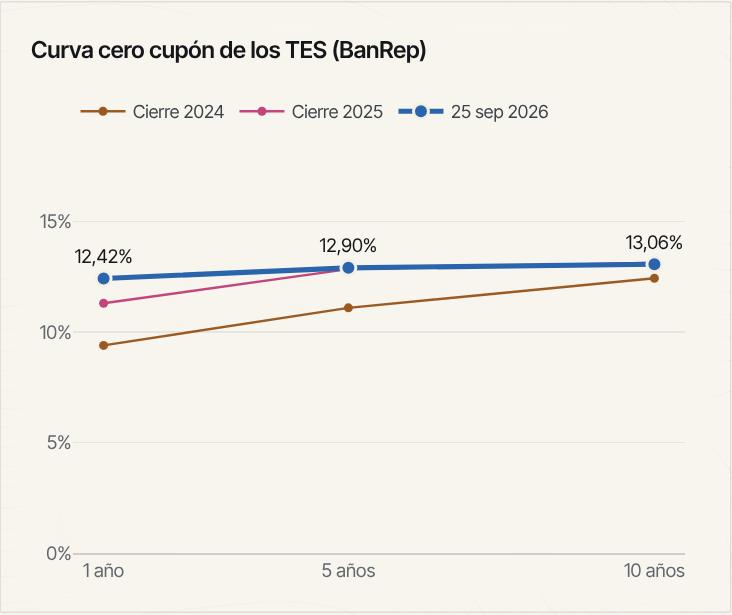
\includegraphics[width=\linewidth,height=0.42\textheight,keepaspectratio]{fig/g-curva-tes.jpg}\end{center}
\paragraph{Qué nos cuenta}
Muestra la curva de rendimientos de los TES (Títulos de Tesorería, los bonos con que el Gobierno nacional se financia en pesos): la tasa que el mercado exige para prestarle al Gobierno a 1, 5 y 10 años. Son tasas cero cupón, es decir, de un pago único al vencimiento, que el Banco de la República estima cada día con el modelo de Nelson y Siegel a partir de las operaciones del SEN y del MEC. La forma de la curva resume cómo el mercado valora el dinero en el tiempo.

\begin{leer}[Cómo se lee]
Eje horizontal: plazo (1, 5 y 10 años); eje vertical: tasa efectiva anual en \%. La línea azul gruesa, con su valor rotulado sobre cada punto, es la curva del día elegido (por defecto, el último dato). Las líneas finas de colores son la curva al cierre de los años marcados (último día hábil de cada año; por defecto, los dos últimos años completos), que se activan o quitan con los botones de años. El selector cambia entre TES en pesos (tasa nominal) y TES en UVR (tasa real); el deslizador y el gráfico de historia cambian la fecha. La escala vertical se fija con el mínimo y el máximo de toda la historia para que las fechas sean comparables.
\end{leer}

\paragraph{Por qué importa}
La curva TES es la referencia con la que se valoran los demás activos en pesos: crédito, bonos corporativos, valoración de empresas y cualquier flujo de caja que se descuente a una tasa. Su nivel refleja el costo de financiación del Gobierno y la postura monetaria; su pendiente, cómo el mercado reparte en el tiempo la remuneración por plazo, inflación y riesgo.

\paragraph{Cómo interpretarlo}
\begin{itemize}
\item Curva normal (creciente): los plazos largos pagan más que los cortos. El tablero la llama normal si la pendiente 10 − 1 años supera 0,3 pp, plana entre 0 y 0,3 pp e invertida si es negativa.
\item Si la curva del día queda por encima de la de un cierre anterior, el costo de endeudarse en pesos subió en todos los plazos; si cambia la inclinación, el movimiento fue distinto en el corto y en el largo plazo.
\item Una curva que baja de izquierda a derecha suele leerse como señal de tasas de política más bajas en el futuro, pero la pendiente también contiene la prima por plazo, que varía con el riesgo y la liquidez.
\item Al pasar el cursor, cada punto muestra su cambio frente al dato más cercano a 365 días antes (si existe uno a menos de 20 días).
\item Son tasas estimadas por un modelo, no precios de bonos individuales: en días de poca negociación pueden reflejar pocas operaciones.
\end{itemize}
\begin{formulas}[Fórmulas]
\formula{Precio de un bono cero cupón}{P = 100 $\div$ (1 + y\textsubscript{n})\textsuperscript{n}}{y\textsubscript{n} = tasa cero cupón efectiva anual al plazo n (en años); P = precio por cada 100 pagados al vencimiento}
\formula{Pendiente}{S\textsubscript{t} = y\textsubscript{10,t} − y\textsubscript{1,t}}{y\textsubscript{10}, y\textsubscript{1} = tasas a 10 y 1 año del día t, en pp}
\formula{Cambio frente a hace un año}{$\Delta$y\textsubscript{n} = y\textsubscript{n,t} − y\textsubscript{n,t−365d}}{t−365d = dato disponible más cercano a 365 días antes, en pp}
\end{formulas}
\begin{metodo}[Metodología]
Tasas cero cupón a 1, 5 y 10 años del día elegido; líneas finas: cierre de cada año marcado.
\par\smallskip{\small\textbf{Fuente:} Banco de la República, curvas cero cupón de los TES (series 15272–15277)}
\end{metodo}

\subsection{Historia de las tasas a 1, 5 y 10 años}
\label{g:g-curva-hist}
\begin{center}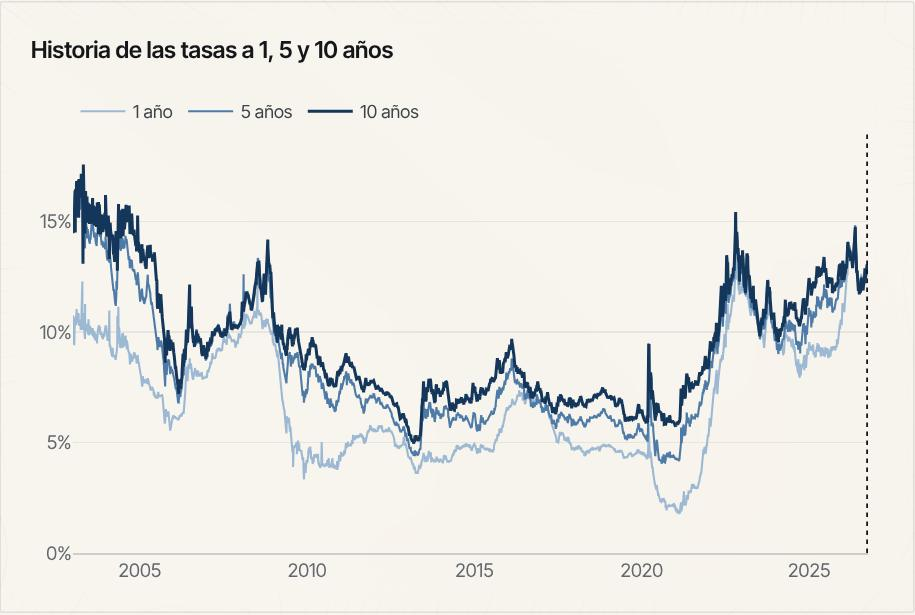
\includegraphics[width=\linewidth,height=0.42\textheight,keepaspectratio]{fig/g-curva-hist.jpg}\end{center}
\paragraph{Qué nos cuenta}
Recorre la historia diaria de las tasas cero cupón de los TES a 1, 5 y 10 años desde 2003. Permite ver los grandes ciclos de tasas en Colombia: periodos de alzas y recortes de la tasa del Banco de la República, episodios de tensión en los mercados y fases en que los plazos largos y cortos se acercan o se separan. Además sirve de control: cada fecha de esta historia alimenta la curva del gráfico vecino.

\begin{leer}[Cómo se lee]
Eje horizontal: fecha (datos diarios); eje vertical: tasa efectiva anual en \%. Tres líneas en tonos de azul: la más clara es el plazo de 1 año, la intermedia el de 5 años y la más oscura y gruesa el de 10 años. Al pasar el cursor se ven las tres tasas del día y la curva vecina se redibuja para esa fecha; un clic la fija (la línea vertical pasa de punteada negra a continua roja) y otro clic la suelta. El selector pesos/UVR cambia ambas gráficas.
\end{leer}

\paragraph{Por qué importa}
Ver los tres plazos juntos distingue los movimientos de la política monetaria, que dominan el corto plazo, de los cambios en la percepción de riesgo fiscal e inflación, que pesan más en el largo plazo. Para un inversionista es la forma más directa de ubicar el nivel actual de tasas frente a su propia historia y de identificar episodios comparables.

\paragraph{Cómo interpretarlo}
\begin{itemize}
\item Si la línea clara (1 año) se mueve mucho más que la oscura (10 años), el movimiento viene de la política monetaria; si las tres se desplazan juntas, cambió el nivel general de las tasas.
\item Cuando la línea clara cruza por encima de la oscura, la curva se invierte; los episodios se detallan en el gráfico «Pendiente y episodios de curva invertida».
\item En la vista UVR las tasas son reales (por encima de la inflación) y por eso son más bajas; la diferencia con la vista en pesos se analiza en la sección de compensación por inflación.
\item Los saltos aislados de un día que se revierten (más de 2 pp) se ocultan en los cálculos derivados; la serie diaria puede tener días sin dato por feriados o falta de operaciones.
\end{itemize}
\begin{formulas}[Fórmulas]
\formula{Tasa cero cupón}{y\textsubscript{n} = (100 $\div$ P\textsubscript{n})\textsuperscript{1/n} − 1}{P\textsubscript{n} = precio de un pago de 100 dentro de n años implícito en la curva estimada; n = 1, 5 o 10}
\end{formulas}
\begin{metodo}[Metodología]
Serie diaria de las tasas cero cupón a 1, 5 y 10 años.
\par\smallskip{\small\textbf{Fuente:} Banco de la República, curvas cero cupón de los TES (series 15272–15277)}
\end{metodo}

\section{Nivel, pendiente y curvatura}

\subsection{Nivel, pendiente y curvatura de la curva en pesos}
\label{g:g-cv-factores}
\begin{center}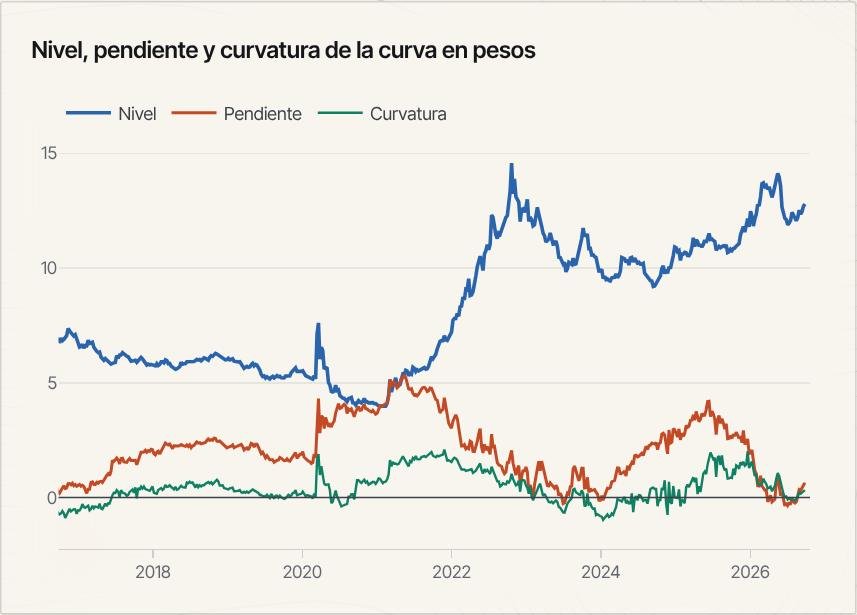
\includegraphics[width=\linewidth,height=0.42\textheight,keepaspectratio]{fig/g-cv-factores.jpg}\end{center}
\paragraph{Qué nos cuenta}
Resume toda la curva de TES en pesos en tres números: el nivel (qué tan altas están las tasas en general), la pendiente (cuánto más pagan los plazos largos que los cortos) y la curvatura (si la parte media de la curva está arqueada hacia arriba o hacia abajo). La literatura (Litterman y Scheinkman, 1991) muestra que estos tres factores explican casi todo el movimiento de una curva de rendimientos.

\begin{leer}[Cómo se lee]
Eje horizontal: fecha, desde 2003; eje vertical en \% para el nivel y en puntos porcentuales (pp) para la pendiente y la curvatura, todos en la misma escala. Línea azul gruesa: nivel; línea naranja: pendiente; línea verde: curvatura. La línea horizontal en cero sirve de referencia para la pendiente y la curvatura. Serie semanal: último dato disponible de cada viernes, calculado con las tasas cero cupón en pesos a 1, 5 y 10 años.
\end{leer}

\paragraph{Por qué importa}
Separar nivel, pendiente y curvatura permite entender qué tipo de movimiento tuvo la curva: un cambio general del costo del dinero, una reacción a la política monetaria que mueve sobre todo el corto plazo o un cambio en la prima que se exige por los plazos largos. Es el lenguaje con que los administradores de portafolios de renta fija miden y cubren su exposición.

\paragraph{Cómo interpretarlo}
\begin{itemize}
\item Nivel al alza: todas las tasas suben (los precios de los TES caen); a la baja, se abaratan las condiciones de financiación en pesos.
\item Pendiente positiva y amplia: curva empinada, con plazos largos que pagan mucho más que los cortos; cerca de cero o negativa: curva plana o invertida.
\item Curvatura positiva: el plazo de 5 años está alto frente al promedio de 1 y 10 años; negativa: la parte media está hundida.
\item Son medidas simples con tres plazos, no factores estimados estadísticamente; el tramo medio de la curva solo se representa con el plazo de 5 años.
\end{itemize}
\begin{formulas}[Fórmulas]
\formula{Nivel}{N\textsubscript{t} = (y\textsubscript{1} + y\textsubscript{5} + y\textsubscript{10}) $\div$ 3}{y\textsubscript{n} = tasa cero cupón en pesos a n años (\%)}
\formula{Pendiente}{S\textsubscript{t} = y\textsubscript{10} − y\textsubscript{1}}{en pp}
\formula{Curvatura}{C\textsubscript{t} = 2 $\times$ y\textsubscript{5} − y\textsubscript{1} − y\textsubscript{10}}{en pp; positiva si el plazo de 5 años está por encima del promedio de los extremos}
\end{formulas}
\begin{metodo}[Metodología]
Factores calculados con las tasas cero cupón en pesos a 1, 5 y 10 años: nivel = promedio; pendiente = 10a − 1a; curvatura = 2$\times$5a − 1a − 10a. Serie semanal (último dato de cada viernes).
\par\smallskip{\small\textbf{Fuente:} Banco de la República, curva cero cupón TES (SEN y MEC, Nelson-Siegel)}
\end{metodo}

\subsection{Pendiente y episodios de curva invertida}
\label{g:g-cv-invertida}
\begin{center}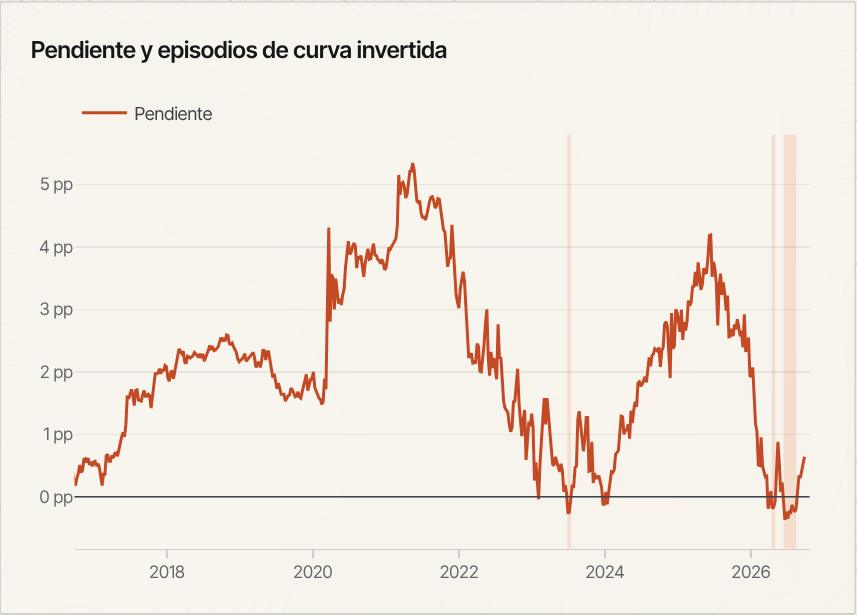
\includegraphics[width=\linewidth,height=0.42\textheight,keepaspectratio]{fig/g-cv-invertida.jpg}\end{center}
\paragraph{Qué nos cuenta}
Sigue la pendiente de la curva de TES en pesos, la diferencia entre la tasa a 10 años y la tasa a 1 año, y marca los periodos en que fue negativa, es decir, en que la curva estuvo invertida: prestarle al Gobierno a un año pagaba más que hacerlo a diez. Las inversiones suelen coincidir con fases de política monetaria restrictiva, cuando la tasa del Banco de la República está alta frente a lo que el mercado considera sostenible.

\begin{leer}[Cómo se lee]
Eje horizontal: fecha, desde 2003; eje vertical: pendiente en puntos porcentuales (pp). La línea naranja es la pendiente semanal (último dato de cada viernes) y la línea horizontal marca el cero. Las franjas naranjas sombreadas señalan los episodios de curva invertida, identificados con datos diarios: tramos de al menos 5 días hábiles seguidos con pendiente negativa. Debajo del gráfico, una tabla lista cada episodio con sus fechas, duración, pendiente mínima y la tasa del Banco al inicio.
\end{leer}

\paragraph{Por qué importa}
La pendiente es uno de los indicadores más seguidos de la estructura de tasas: la literatura (Estrella y Hardouvelis, 1991) documenta su contenido informativo sobre la actividad económica. Una curva invertida indica que el mercado exige más por el corto plazo que por el largo, algo que afecta el margen de los bancos (que se fondean a corto y prestan a largo) y las decisiones de financiación de empresas y Gobierno.

\paragraph{Cómo interpretarlo}
\begin{itemize}
\item Pendiente positiva y creciente: la curva se empina; cerca de cero: curva plana; bajo cero: curva invertida (franja sombreada).
\item Una inversión breve puede deberse a un movimiento puntual del plazo de 1 año; los episodios largos y profundos son los relevantes, por eso se exige un mínimo de 5 días hábiles.
\item Conviene leerla junto con la tasa del Banco (gráfico «TES frente a la tasa del Banco»): las inversiones suelen aparecer cuando la tasa de política está en niveles altos.
\item La relación entre curva invertida y desaceleración documentada en otros países no es mecánica; en Colombia también influyen la prima por plazo, el riesgo fiscal y los flujos de inversionistas extranjeros.
\end{itemize}
\begin{formulas}[Fórmulas]
\formula{Pendiente}{S\textsubscript{t} = y\textsubscript{10,t} − y\textsubscript{1,t}}{y\textsubscript{10}, y\textsubscript{1} = tasas cero cupón en pesos a 10 y 1 año, en pp}
\formula{Episodio invertido}{S\textsubscript{d} < 0 durante k $\ge$ 5 días hábiles consecutivos}{d = día hábil con dato; k = longitud del tramo}
\end{formulas}
\begin{metodo}[Metodología]
Episodios: tramos de al menos 5 días hábiles consecutivos con pendiente 10a − 1a negativa (datos diarios).
\par\smallskip{\small\textbf{Fuente:} Banco de la República, curva cero cupón TES (SEN y MEC, Nelson-Siegel)}
\end{metodo}

\section{¿Cómo se ha movido la curva?}

\subsection{Cambio de cada plazo (puntos básicos)}
\label{g:g-cv-cambios}
\begin{center}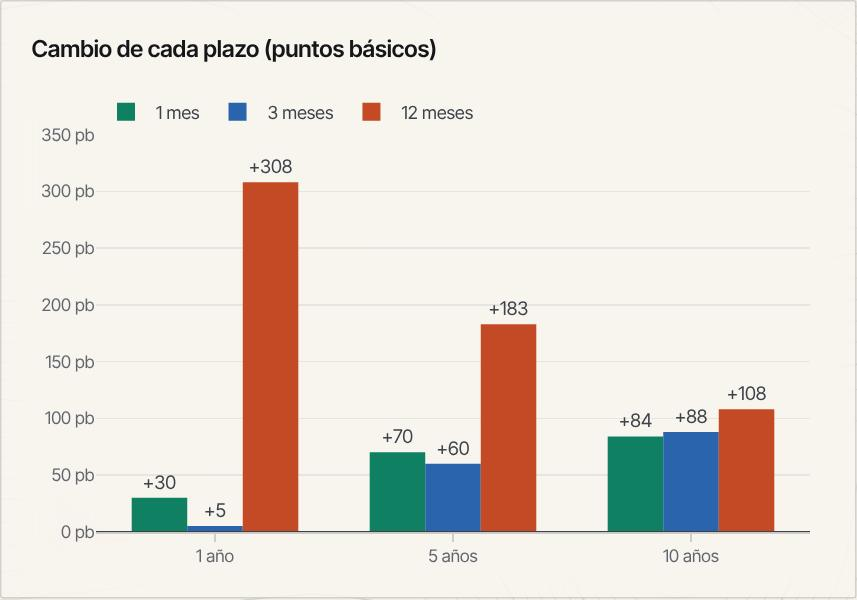
\includegraphics[width=\linewidth,height=0.42\textheight,keepaspectratio]{fig/g-cv-cambios.jpg}\end{center}
\paragraph{Qué nos cuenta}
Muestra cuánto se movió la tasa cero cupón de los TES en pesos en cada plazo (1, 5 y 10 años) durante el último mes, los últimos tres meses y el último año. Permite ver de un vistazo si las tasas subieron o bajaron y si el movimiento fue parejo a lo largo de la curva o se concentró en el corto o en el largo plazo.

\begin{leer}[Cómo se lee]
Eje horizontal: plazo (1, 5 y 10 años); eje vertical: cambio en puntos básicos (pb; 100 pb = 1 punto porcentual). Para cada plazo hay tres barras: verde para el cambio en 1 mes, azul para 3 meses y naranja para 12 meses, con su valor rotulado. La línea horizontal marca el cero: las barras hacia arriba indican alzas de tasa y hacia abajo, bajas. La comparación se hace contra el último día hábil disponible en o antes de la fecha de hace 1, 3 y 12 meses.
\end{leer}

\paragraph{Por qué importa}
Los cambios de tasas determinan la rentabilidad de quien tiene TES: cuando la tasa sube, el precio del bono cae, y la caída es mayor cuanto más largo es el plazo. Además, el patrón por plazos revela la causa probable del movimiento (política monetaria, inflación o riesgo), información útil para gestionar la duración de un portafolio y el costo de financiación de empresas y Gobierno.

\paragraph{Cómo interpretarlo}
\begin{itemize}
\item Alza con empinamiento: las tasas suben más en el largo plazo; alza con aplanamiento: suben más en el corto. Las bajas se leen igual en sentido contrario.
\item Si las barras de 1 mes y de 12 meses tienen signos distintos, el movimiento reciente va en contra de la tendencia del año.
\item Como referencia, la sensibilidad del precio de un bono cero cupón es aproximadamente su plazo: un alza de 100 pb a 10 años reduce su precio cerca de 10\%.
\item Son diferencias entre dos días puntuales: un dato atípico en cualquiera de las dos fechas altera el resultado.
\end{itemize}
\begin{formulas}[Fórmulas]
\formula{Cambio en pb}{$\Delta$\textsubscript{h}y\textsubscript{n} = (y\textsubscript{n,t} − y\textsubscript{n,t−h}) $\times$ 100}{y\textsubscript{n,t} = tasa en pesos a n años del último día (\%); t−h = último día hábil en o antes de hace h = 1, 3 o 12 meses}
\formula{Efecto aproximado en precio}{$\Delta$P $\div$ P $\approx$ −D $\times$ $\Delta$y}{D = duración modificada ($\approx$ n $\div$ (1 + y) en un cero cupón); $\Delta$y en tanto por uno}
\end{formulas}
\begin{metodo}[Metodología]
Diferencia entre la tasa cero cupón del último día y la del último día hábil disponible hace 1, 3 y 12 meses, en puntos básicos.
\par\smallskip{\small\textbf{Fuente:} Banco de la República, curva cero cupón TES (SEN y MEC, Nelson-Siegel)}
\end{metodo}

\subsection{¿Tasa real o inflación? Cambio en 12 meses}
\label{g:g-cv-descomposicion}
\begin{center}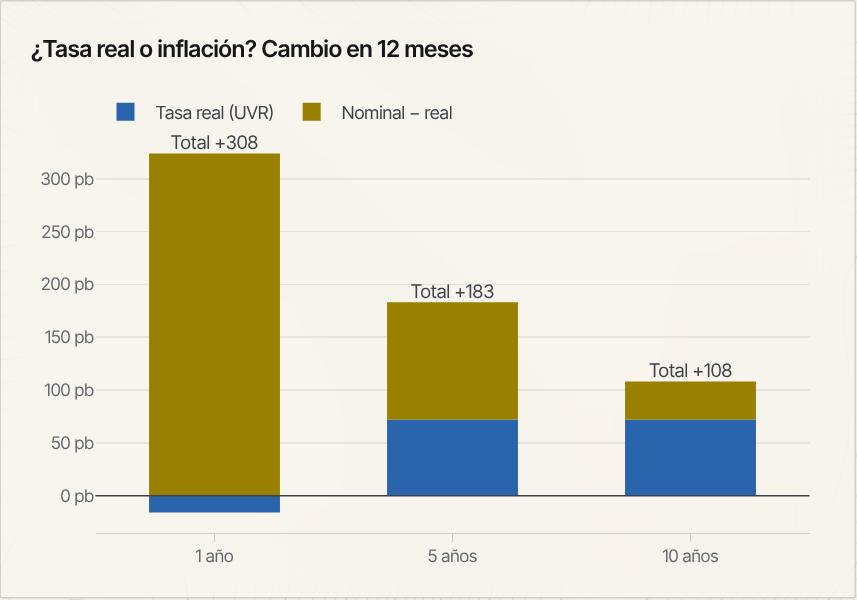
\includegraphics[width=\linewidth,height=0.42\textheight,keepaspectratio]{fig/g-cv-descomposicion.jpg}\end{center}
\paragraph{Qué nos cuenta}
Separa el cambio de las tasas de los TES en pesos durante el último año en dos partes: la que vino de la tasa real, medida con los TES en UVR (Unidad de Valor Real, una unidad de cuenta que se ajusta con la inflación), y la que vino de la diferencia entre la tasa nominal y la real, que aproxima la compensación por inflación. Responde si las tasas se movieron porque cambió el costo real del dinero o porque cambió la inflación que el mercado incorpora.

\begin{leer}[Cómo se lee]
Eje horizontal: plazo (1, 5 y 10 años); eje vertical: cambio en 12 meses en puntos básicos (pb). Las barras están apiladas: azul, cambio de la tasa real (TES UVR); amarillo, cambio de la diferencia nominal − real. Sobre cada plazo, el rótulo «Total» indica el cambio de la tasa en pesos, que es la suma de las dos barras. Las barras por debajo de cero restan; la línea horizontal marca el cero. La comparación es contra el último día hábil disponible hace 12 meses.
\end{leer}

\paragraph{Por qué importa}
Un alza de tasas nominales por mayor inflación esperada tiene implicaciones distintas que un alza de la tasa real: la primera afecta el poder adquisitivo y la credibilidad de la meta de inflación; la segunda endurece las condiciones financieras de verdad, encarece la inversión y suele asociarse a política monetaria o a primas de riesgo. Esta distinción es clave para leer la curva más allá de su nivel.

\paragraph{Cómo interpretarlo}
\begin{itemize}
\item Barra azul dominante: el movimiento vino de la tasa real (política monetaria, riesgo país, demanda de bonos); barra amarilla dominante: vino de la compensación por inflación.
\item Barras de signo opuesto indican que la tasa real y la compensación se compensaron parcialmente; el «Total» muestra el efecto neto.
\item La diferencia nominal − real es una aproximación lineal de la compensación de Fisher; para la cifra exacta ver el gráfico «Nominal = real + compensación por inflación».
\item La compensación incluye primas por riesgo inflacionario y por liquidez (los TES UVR se negocian menos), así que no equivale a la inflación esperada pura.
\end{itemize}
\begin{formulas}[Fórmulas]
\formula{Descomposición}{$\Delta$y\textsubscript{n}\textsuperscript{\$} = $\Delta$r\textsubscript{n} + $\Delta$(y\textsubscript{n}\textsuperscript{\$} − r\textsubscript{n})}{y\textsuperscript{\$} = tasa TES en pesos; r = tasa TES en UVR; $\Delta$ = cambio en 12 meses, en pb}
\formula{Brecha nominal − real}{B\textsubscript{n} = y\textsubscript{n}\textsuperscript{\$} − r\textsubscript{n}}{n = 1, 5 o 10 años; aproximación de la compensación por inflación}
\end{formulas}
\begin{metodo}[Metodología]
Cambio en 12 meses de la tasa en pesos = cambio de la tasa UVR (real) + cambio de la diferencia nominal − real.
\par\smallskip{\small\textbf{Fuente:} Banco de la República, curva cero cupón TES (SEN y MEC, Nelson-Siegel)}
\end{metodo}

\section{Tasa nominal, tasa real y compensación por inflación}

\subsection{Nominal = real + compensación por inflación (hoy)}
\label{g:g-cv-fisher}
\begin{center}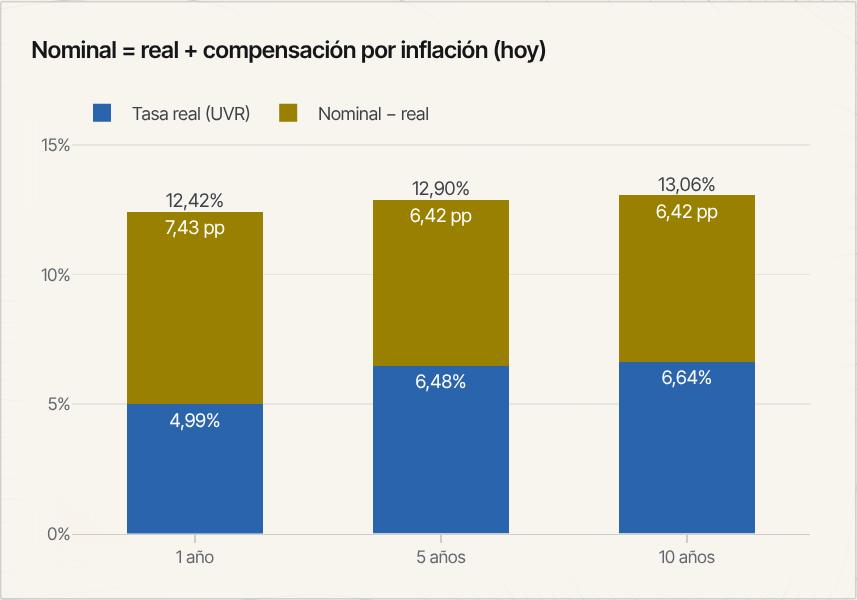
\includegraphics[width=\linewidth,height=0.42\textheight,keepaspectratio]{fig/g-cv-fisher.jpg}\end{center}
\paragraph{Qué nos cuenta}
Descompone la tasa de los TES en pesos del último día en sus dos componentes según la ecuación de Fisher: la tasa real, que pagan los TES en UVR por encima de la inflación, y lo que falta para llegar a la tasa nominal, que es la compensación que el mercado exige por la inflación (más primas por riesgo y liquidez). Se presenta para los plazos de 1, 5 y 10 años.

\begin{leer}[Cómo se lee]
Eje horizontal: plazo (1, 5 y 10 años); eje vertical: tasa en \%, empezando en cero. Cada barra apilada tiene una parte azul, la tasa real del TES UVR (rotulada en \%), y una parte amarilla, la diferencia hasta la tasa del TES en pesos (rotulada en pp). El número sobre cada barra es la tasa nominal en pesos. Al pasar el cursor por la parte amarilla aparece la compensación por inflación exacta de Fisher, que difiere levemente de la resta simple.
\end{leer}

\paragraph{Por qué importa}
Un inversionista que compra TES en pesos asume el riesgo de inflación; uno que compra TES UVR, no. Comparar ambas tasas muestra cuánta inflación tendría que ocurrir para que las dos inversiones rindan igual, una referencia para elegir entre instrumentos nominales e indexados y para evaluar la credibilidad de la meta de inflación del 3\% del Banco de la República.

\paragraph{Cómo interpretarlo}
\begin{itemize}
\item Parte amarilla grande frente a la meta de 3\%: el mercado incorpora inflación alta o exige una prima elevada por el riesgo inflacionario.
\item Si la parte amarilla crece con el plazo, la compensación por inflación es mayor a largo plazo; si se reduce, el mercado incorpora inflación decreciente.
\item La parte azul alta indica condiciones financieras reales restrictivas: el dinero es caro aun descontando la inflación.
\item El eje empieza en cero: en periodos en que alguna tasa real fue negativa, esa parte no se vería; la compensación incluye primas, por lo que no es la inflación esperada pura.
\end{itemize}
\begin{formulas}[Fórmulas]
\formula{Ecuación de Fisher}{(1 + y\textsubscript{n}\textsuperscript{\$}) = (1 + r\textsubscript{n}) $\times$ (1 + $\pi$\textsubscript{n}\textsuperscript{e})}{y\textsuperscript{\$} = tasa TES en pesos; r = tasa TES UVR; $\pi$\textsuperscript{e} = compensación por inflación (todo en tanto por uno)}
\formula{Compensación exacta}{$\pi$\textsubscript{n}\textsuperscript{e} = (1 + y\textsubscript{n}\textsuperscript{\$}) $\div$ (1 + r\textsubscript{n}) − 1}{se muestra en el recuadro flotante}
\formula{Diferencia apilada}{B\textsubscript{n} = y\textsubscript{n}\textsuperscript{\$} − r\textsubscript{n}}{altura de la parte amarilla, en pp; B $\approx$ $\pi$\textsuperscript{e} para tasas bajas}
\end{formulas}
\begin{metodo}[Metodología]
Tasa UVR más la diferencia hasta la tasa en pesos. La compensación por inflación exacta es (1 + nominal)/(1 + real) − 1 (Fisher) e incluye primas por riesgo y liquidez.
\par\smallskip{\small\textbf{Fuente:} Banco de la República, curva cero cupón TES (SEN y MEC, Nelson-Siegel)}
\end{metodo}

\subsection{Tasa real y compensación por inflación a 10 años}
\label{g:g-cv-real}
\begin{center}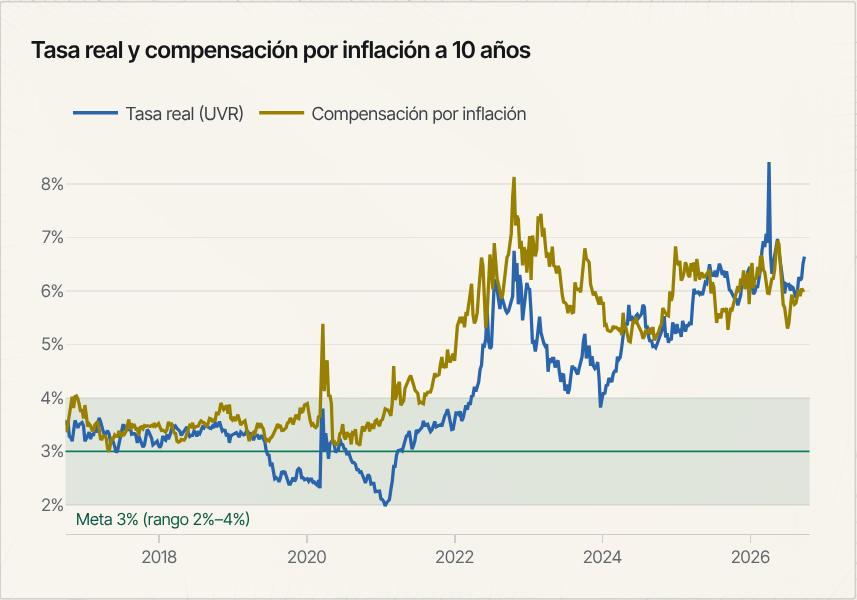
\includegraphics[width=\linewidth,height=0.42\textheight,keepaspectratio]{fig/g-cv-real.jpg}\end{center}
\paragraph{Qué nos cuenta}
Sigue en el tiempo los dos componentes de la tasa de los TES a 10 años: la tasa real que pagan los TES en UVR y la compensación por inflación implícita, que surge de comparar los TES en pesos con los TES UVR mediante la ecuación de Fisher. Muestra si el costo real del endeudamiento de largo plazo y la inflación que el mercado incorpora a diez años se han movido juntos o en direcciones distintas.

\begin{leer}[Cómo se lee]
Eje horizontal: fecha, desde 2003; eje vertical: \% anual. Línea azul: tasa cero cupón del TES UVR a 10 años (tasa real). Línea amarilla: compensación por inflación a 10 años. La franja verde marca el rango meta del Banco de la República (2\% a 4\%) y la línea verde, la meta puntual de 3\%: es la referencia para la línea amarilla. Serie semanal (último dato de cada viernes).
\end{leer}

\paragraph{Por qué importa}
La tasa real de largo plazo es el costo de financiación relevante para la inversión en infraestructura, vivienda y empresas, y una medida de la prima que se exige al riesgo soberano colombiano. La compensación por inflación a 10 años indica si el mercado confía en que la inflación converja a la meta en el largo plazo, un factor central de la credibilidad del Banco de la República.

\paragraph{Cómo interpretarlo}
\begin{itemize}
\item Línea amarilla dentro de la franja verde: la compensación de largo plazo es coherente con la meta; por encima de 4\%, el mercado incorpora inflación o primas de riesgo inflacionario elevadas.
\item Si la línea azul sube mientras la amarilla se mantiene, el encarecimiento del crédito a largo plazo es real (riesgo fiscal, tasas globales o política monetaria), no inflacionario.
\item La suma aproximada de ambas líneas da la tasa del TES en pesos a 10 años; la descomposición de los cambios recientes está en «¿Tasa real o inflación?».
\item La compensación contiene primas por riesgo inflacionario y por liquidez de los TES UVR; el gráfico de la página de inflación «Inflación esperada a largo plazo» aísla el tramo de 5 a 10 años.
\end{itemize}
\begin{formulas}[Fórmulas]
\formula{Compensación por inflación a 10 años}{$\pi$\textsubscript{10} = [(1 + y\textsubscript{10}\textsuperscript{\$}) $\div$ (1 + r\textsubscript{10}) − 1] $\times$ 100}{y\textsuperscript{\$}\textsubscript{10} = tasa cero cupón en pesos a 10 años; r\textsubscript{10} = tasa cero cupón UVR a 10 años (tanto por uno)}
\formula{Serie semanal}{x\textsubscript{s} = x\textsubscript{d*}}{d* = último día con dato de la semana que termina el viernes s}
\end{formulas}
\begin{metodo}[Metodología]
Tasa cero cupón UVR a 10 años y compensación por inflación implícita (Fisher) a 10 años. Serie semanal.
\par\smallskip{\small\textbf{Fuente:} Banco de la República, curva cero cupón TES (SEN y MEC, Nelson-Siegel)}
\end{metodo}

\section{Prima sobre la tasa del Banco y volatilidad}

\subsection{TES frente a la tasa del Banco}
\label{g:g-cv-prima}
\begin{center}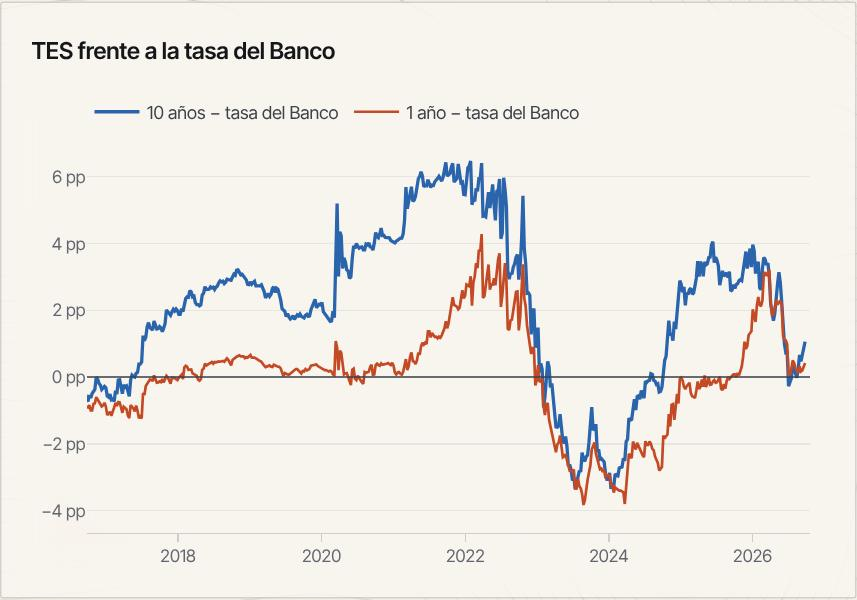
\includegraphics[width=\linewidth,height=0.42\textheight,keepaspectratio]{fig/g-cv-prima.jpg}\end{center}
\paragraph{Qué nos cuenta}
Compara las tasas de los TES en pesos a 1 y a 10 años con la tasa de política monetaria (TPM), la tasa con la que el Banco de la República presta liquidez a los bancos a un día. La diferencia indica cuánto más (o menos) que la tasa del Banco exige el mercado por prestarle al Gobierno a esos plazos, y refleja tanto lo que el mercado espera de la política monetaria como las primas por plazo y por riesgo.

\begin{leer}[Cómo se lee]
Eje horizontal: fecha, desde 2003; eje vertical: diferencia en puntos porcentuales (pp). Línea azul: TES a 10 años menos la TPM. Línea naranja: TES a 1 año menos la TPM. La línea horizontal marca el cero: por encima, el TES rinde más que la tasa del Banco; por debajo, menos. Se usa la TPM vigente cada día y la serie es semanal (último dato de cada viernes).
\end{leer}

\paragraph{Por qué importa}
La TPM es el ancla de corto plazo de todo el sistema de tasas; la distancia de los TES frente a ella mide cómo se transmite la política monetaria a los plazos largos, que son los que importan para el crédito hipotecario, la inversión y el costo de la deuda pública. Un diferencial amplio a 10 años encarece la financiación de largo plazo aun cuando el Banco recorta su tasa.

\paragraph{Cómo interpretarlo}
\begin{itemize}
\item Diferencial de 1 año negativo: el mercado incorpora recortes de la TPM en los próximos meses; positivo: incorpora alzas o exige prima.
\item Diferencial de 10 años alto y creciente: mayor prima por plazo o por riesgo fiscal, o expectativa de tasas más altas a largo plazo.
\item Las dos líneas suelen caer cuando el Banco sube la TPM (el denominador común se mueve primero) y subir cuando la recorta; conviene leerlas junto con el gráfico de la tasa de política en la página de tasas.
\item La TPM cambia en saltos discretos en las reuniones de la Junta Directiva, mientras los TES se mueven a diario; los cambios bruscos del diferencial suelen coincidir con esas decisiones.
\end{itemize}
\begin{formulas}[Fórmulas]
\formula{Diferencial frente a la TPM}{Sp\textsubscript{n,t} = y\textsubscript{n,t} − TPM\textsubscript{t}}{y\textsubscript{n} = tasa cero cupón en pesos a n = 1 o 10 años; TPM\textsubscript{t} = tasa de política vigente el día t; en pp}
\end{formulas}
\begin{metodo}[Metodología]
Tasa cero cupón en pesos menos la tasa de política monetaria vigente ese día, en puntos porcentuales. Serie semanal.
\par\smallskip{\small\textbf{Fuente:} Banco de la República (curva cero cupón TES y tasa de política monetaria)}
\end{metodo}

\subsection{Volatilidad del TES a 10 años}
\label{g:g-cv-volatilidad}
\begin{center}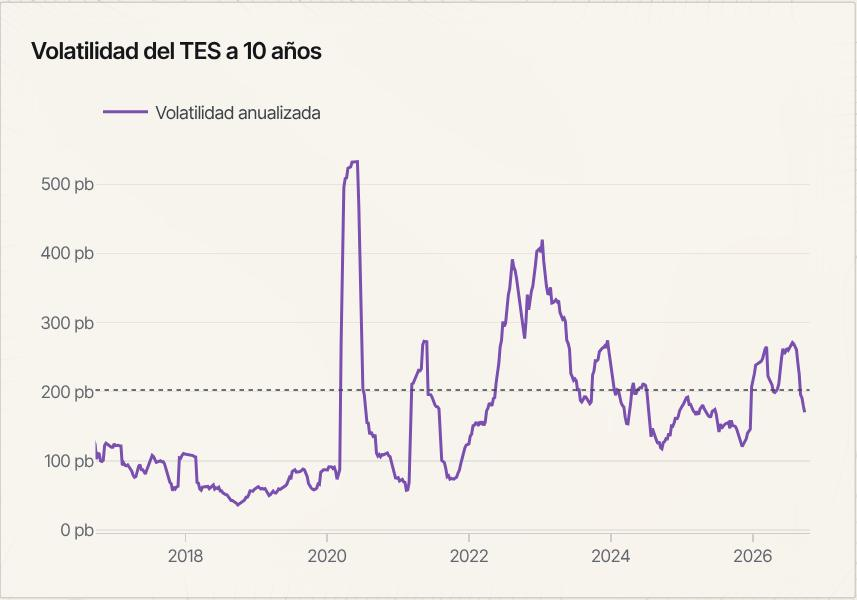
\includegraphics[width=\linewidth,height=0.42\textheight,keepaspectratio]{fig/g-cv-volatilidad.jpg}\end{center}
\paragraph{Qué nos cuenta}
Mide qué tan bruscos han sido los movimientos diarios de la tasa del TES a 10 años: es la desviación estándar de sus cambios diarios durante los últimos 60 días hábiles (unos tres meses), expresada en términos anuales. Sirve como termómetro del riesgo de mercado de la deuda pública colombiana y de la incertidumbre de los inversionistas.

\begin{leer}[Cómo se lee]
Eje horizontal: fecha, desde 2003; eje vertical: volatilidad anualizada en puntos básicos (pb). La línea morada es la volatilidad móvil de 60 días hábiles, mostrada semanalmente (último dato de cada viernes). La línea punteada gris horizontal es el promedio de toda la serie desde 2003, la referencia para saber si el mercado está más o menos agitado que lo habitual. Se exige un mínimo de 48 cambios diarios en la ventana para calcular cada punto.
\end{leer}

\paragraph{Por qué importa}
La volatilidad determina el riesgo de mantener TES: con mayor volatilidad, las pérdidas o ganancias de valoración en un periodo dado pueden ser mayores, lo que lleva a fondos y bancos a reducir posiciones o exigir más prima. Los picos suelen coincidir con choques globales, episodios de riesgo fiscal o salidas de inversionistas extranjeros, y afectan el costo de financiación del Gobierno.

\paragraph{Cómo interpretarlo}
\begin{itemize}
\item Por encima de la línea punteada: el mercado de TES está más agitado que su promedio histórico; por debajo, más calmado.
\item Un pico aislado indica un choque puntual; una volatilidad alta persistente refleja incertidumbre prolongada sobre inflación, política monetaria o finanzas públicas.
\item Como orden de magnitud, una volatilidad anualizada de 100 pb equivale a una desviación diaria de unos 6 pb (100 $\div$ $\surd$252).
\item Es una medida histórica (mira hacia atrás) y reacciona con rezago; los saltos aislados de un día que se revierten se depuran antes del cálculo.
\end{itemize}
\begin{formulas}[Fórmulas]
\formula{Cambio diario}{$\Delta$y\textsubscript{d} = (y\textsubscript{10,d} − y\textsubscript{10,d−1}) $\times$ 100}{y\textsubscript{10} = tasa cero cupón en pesos a 10 años (\%); en pb}
\formula{Volatilidad anualizada}{$\sigma$\textsubscript{t} = $\surd$252 $\times$ $\surd$[$\Sigma$ ($\Delta$y\textsubscript{d} − $\Delta\bar{y}$)\textsuperscript{2} $\div$ (k − 1)]}{suma sobre los k $\le$ 60 últimos días hábiles (mínimo 48); $\Delta\bar{y}$ = promedio de esos cambios; 252 = días hábiles por año}
\end{formulas}
\begin{metodo}[Metodología]
Desviación estándar móvil de 60 días hábiles de los cambios diarios de la tasa a 10 años, $\times$ $\surd$252, en puntos básicos. La línea punteada es el promedio desde 2003.
\par\smallskip{\small\textbf{Fuente:} Banco de la República, curva cero cupón TES (SEN y MEC, Nelson-Siegel)}
\end{metodo}

\section*{Lecturas de la página}
\begin{itemize}\small
\item \textbf{Fisher, I. (1930). The Theory of Interest. Macmillan.} Tasa nominal = tasa real + compensación por inflación.
\item \textbf{Nelson, C. R. y Siegel, A. F. (1987). Parsimonious Modeling of Yield Curves. Journal of Business, 60(4), 473–489.} Modelo con el que el Banco de la República estima la curva cero cupón de los TES.
\item \textbf{Litterman, R. y Scheinkman, J. (1991). Common Factors Affecting Bond Returns. Journal of Fixed Income, 1(1), 54–61.} Nivel, pendiente y curvatura explican casi todo el movimiento de la curva.
\item \textbf{Estrella, A. y Hardouvelis, G. A. (1991). The Term Structure as a Predictor of Real Economic Activity. Journal of Finance, 46(2), 555–576.} El contenido informativo de la pendiente de la curva.
\item \textbf{Gürkaynak, R. S., Sack, B. y Wright, J. H. (2010). The TIPS Yield Curve and Inflation Compensation. American Economic Journal: Macroeconomics, 2(1), 70–92.} Por qué la compensación por inflación incluye primas además de la inflación esperada.
\item \textbf{Arango, L. E., Melo, L. F. y Vásquez, D. M. (2002). Estimación de la estructura a plazo de las tasas de interés en Colombia. Borradores de Economía 196, Banco de la República.} Estimación de la curva cero cupón colombiana.
\item \textbf{Espinosa, J. A., Melo, L. F. y Moreno, J. F. (2014). Estimación de la prima por vencimiento de los TES en pesos del gobierno colombiano. Borradores de Economía 854, Banco de la República.} La prima por plazo de los TES crece y se vuelve más volátil con el vencimiento.
\end{itemize}

\chapter{Tasa de cambio}
\label{atlas:mercados}

{\large\sffamily\bfseries El peso colombiano\par}\medskip

El peso frente al dólar y a otras monedas, la tasa de cambio real y lo que mueve al peso: el dólar global, el petróleo y los flujos de divisas.

{\small\color{cmmuted}Página del sitio: \url{https://stv-quant.github.io/ColombiaMacro-USBCali/mercados/}}

\section{¿Cómo está el peso frente al dólar?}

\subsection{Pesos por dólar (TRM)}
\label{g:g-dolar}
\begin{center}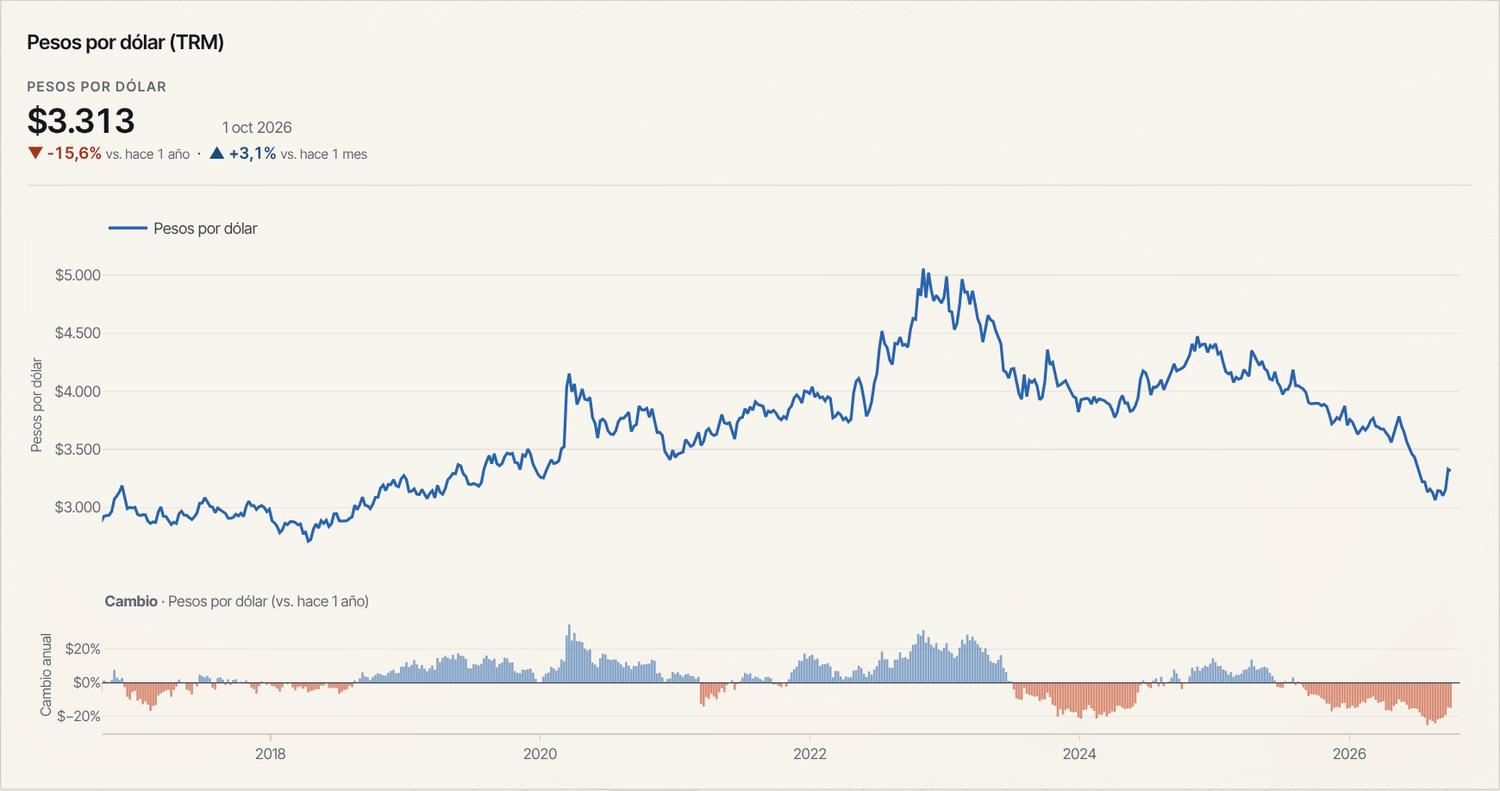
\includegraphics[width=\linewidth,height=0.42\textheight,keepaspectratio]{fig/g-dolar.jpg}\end{center}
\paragraph{Qué nos cuenta}
Muestra cuántos pesos cuesta un dólar según la Tasa Representativa del Mercado (TRM), el precio de referencia del dólar en Colombia que calcula y certifica la Superintendencia Financiera con las operaciones del mercado cambiario. Colombia tiene un régimen de tasa de cambio flexible: el precio lo determinan la oferta y la demanda de dólares, no una autoridad.

\begin{leer}[Cómo se lee]
Panel superior: pesos por dólar, con el último dato de cada semana; si la línea sube, el peso se debilita (se necesitan más pesos por dólar) y si baja, se fortalece. Panel inferior: barras con la variación porcentual frente a la misma semana un año antes, azules cuando la TRM sube (peso más débil) y naranjas cuando baja (peso más fuerte). Vista inicial de diez años, ajustable con el selector de horizonte.
\end{leer}

\paragraph{Por qué importa}
La tasa de cambio afecta los precios de los bienes importados y, por tanto, la inflación; el valor en pesos de la deuda externa de empresas y gobierno; los ingresos de exportadores y receptores de remesas; y el rendimiento en dólares de cualquier inversión en activos colombianos. Es uno de los precios más vigilados por inversionistas extranjeros y por el Banco de la República.

\paragraph{Cómo interpretarlo}
\begin{itemize}
\item Una variación anual de +10\% significa que el dólar cuesta 10\% más en pesos que hace un año: el peso se depreció.
\item Para saber si el movimiento es propio de Colombia o global, compare con el dólar global y con las monedas vecinas en los gráficos de esta página.
\item El precio del petróleo, el apetito global por riesgo y el diferencial de tasas de interés con Estados Unidos son factores que suelen acompañar los grandes movimientos de la TRM.
\item Una depreciación encarece los bienes importados con rezago; la transmisión a la inflación suele ser parcial.
\item La TRM calculada con las operaciones de un día rige al día hábil siguiente; cada punto del gráfico es el último valor vigente de la semana.
\end{itemize}
\begin{formulas}[Fórmulas]
\formula{Variación anual}{g\textsubscript{t} = (TRM\textsubscript{t} $\div$ TRM\textsubscript{t−52} − 1) $\times$ 100}{TRM\textsubscript{t} = último valor de la semana t; t−52 = misma semana un año antes}
\formula{TRM (cálculo de la Superfinanciera)}{TRM = $\Sigma$\textsubscript{k} (p\textsubscript{k} $\times$ m\textsubscript{k}) $\div$ $\Sigma$\textsubscript{k} m\textsubscript{k}}{p\textsubscript{k} = tasa de la operación de contado k entre pesos y dólares; m\textsubscript{k} = su monto en dólares}
\end{formulas}
\begin{metodo}[Metodología]
Pesos por dólar, último dato de cada semana. Panel inferior: variación porcentual frente a un año antes.
\par\smallskip{\small\textbf{Fuente:} Banco de la República, Tasa Representativa del Mercado (TRM), certificada por la Superfinanciera}
\end{metodo}

\subsection{Tasa de cambio real (2010 = 100)}
\label{g:g-itcr}
\begin{center}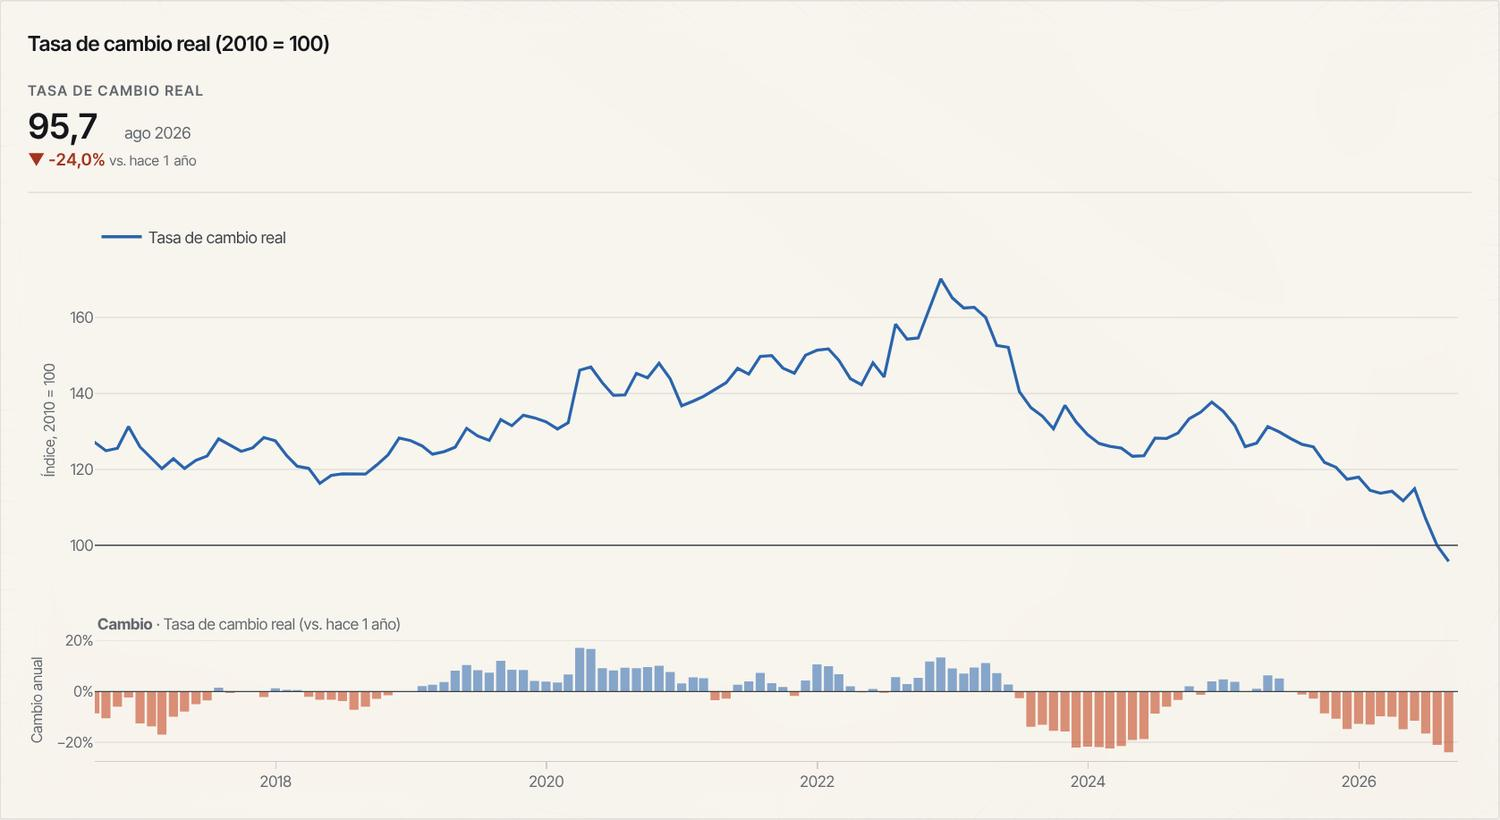
\includegraphics[width=\linewidth,height=0.42\textheight,keepaspectratio]{fig/g-itcr.jpg}\end{center}
\paragraph{Qué nos cuenta}
Muestra el Índice de la Tasa de Cambio Real (ITCR) que calcula el Banco de la República: la tasa de cambio del peso frente a las monedas de sus principales socios comerciales, ajustada por la diferencia de inflación (medida con el IPC). Indica si los bienes colombianos son caros o baratos frente a los de otros países, algo que la TRM sola no muestra.

\begin{leer}[Cómo se lee]
Panel superior: el índice mensual con base 2010 = 100; la línea horizontal marca 100. Por encima de 100, el peso está más barato en términos reales que en 2010; por debajo, más caro. Panel inferior: barras con la variación porcentual frente al mismo mes del año anterior, azules cuando el índice sube (el peso se abarata en términos reales) y naranjas cuando baja. Vista inicial de diez años.
\end{leer}

\paragraph{Por qué importa}
Un peso real barato mejora la competitividad de exportadores y de quienes compiten con importaciones, y encarece lo importado; uno caro abarata importaciones y viajes, pero resta competitividad. La tasa de cambio real es una variable central para entender el ajuste de la balanza de pagos y la rentabilidad relativa de producir en Colombia.

\paragraph{Cómo interpretarlo}
\begin{itemize}
\item Sube = depreciación real (el peso se abarata frente a sus socios después de corregir por inflación); baja = apreciación real.
\item El año base 2010 es solo una fecha de comparación, no un nivel de equilibrio: estar por encima o por debajo de 100 no indica por sí solo desalineación.
\item Si la TRM sube pero la inflación colombiana es mayor que la de los socios, el ITCR puede subir menos que la TRM o incluso bajar.
\item Para la comparación con el promedio histórico y con la competitividad en Estados Unidos, vea los gráficos de tasa de cambio real de esta página.
\item Los datos se revisan cuando se actualizan los índices de precios y las ponderaciones de los socios.
\end{itemize}
\begin{formulas}[Fórmulas]
\formula{Tasa de cambio real (esquema)}{ITCR\textsubscript{t} = $\Pi$\textsubscript{j} (E\textsubscript{j,t} $\times$ P\textsuperscript{*}\textsubscript{j,t} $\div$ P\textsubscript{t})\textsuperscript{w\textsubscript{j}}, base 2010 = 100}{E\textsubscript{j} = pesos por unidad de la moneda del socio j; P\textsuperscript{*}\textsubscript{j} = IPC del socio j; P = IPC de Colombia; w\textsubscript{j} = peso del socio en el comercio}
\formula{Variación anual}{g\textsubscript{t} = (ITCR\textsubscript{t} $\div$ ITCR\textsubscript{t−12} − 1) $\times$ 100}{t = mes}
\end{formulas}
\begin{metodo}[Metodología]
Tasa de cambio ajustada por la inflación de Colombia frente a la de sus socios comerciales. Por encima de 100 el peso está más barato (en términos reales) que en el año base.
\par\smallskip{\small\textbf{Fuente:} Banco de la República, Índice de la Tasa de Cambio Real (ITCR-IPC)}
\end{metodo}

\section{¿Es el peso o es el dólar?}

\subsection{Cambio frente al dólar en 12 meses}
\label{g:g-tc-pares}
\begin{center}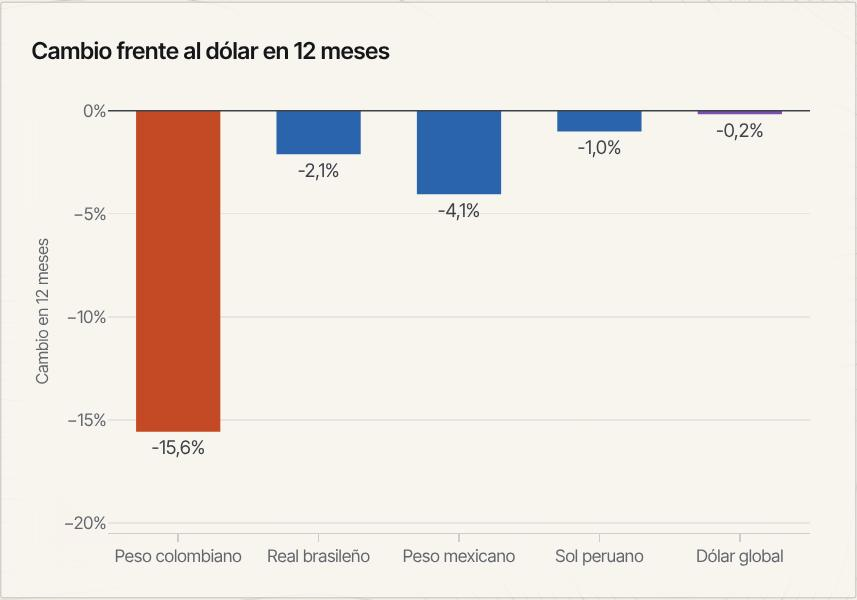
\includegraphics[width=\linewidth,height=0.42\textheight,keepaspectratio]{fig/g-tc-pares.jpg}\end{center}
\paragraph{Qué nos cuenta}
Compara cuánto cambió en los últimos 12 meses el valor del dólar en pesos colombianos con lo que cambió frente al real brasileño, el peso mexicano y el sol peruano, y con el índice amplio del dólar de la Reserva Federal. Sirve para separar lo que es propio de Colombia de lo que es un movimiento general del dólar o de las monedas de la región.

\begin{leer}[Cómo se lee]
Una barra por moneda con la variación porcentual de las unidades de esa moneda por dólar entre el último dato y el último disponible 12 meses antes. Positivo = la moneda se debilita frente al dólar; negativo = se fortalece. Naranja: peso colombiano; azul: monedas vecinas; morado: «dólar global», el índice amplio nominal de la Reserva Federal frente a 26 monedas, que se lee al revés (positivo = el dólar se fortalece en el mundo).
\end{leer}

\paragraph{Por qué importa}
Si el peso se mueve como sus vecinos y como el dólar global, el origen del movimiento es externo (tasas de interés en Estados Unidos, apetito global por riesgo, precios de materias primas). Si se separa, pesan más factores locales: política fiscal y monetaria, flujos de inversión o percepción de riesgo del país. Esta distinción es clave para interpretar el riesgo cambiario de una inversión en Colombia.

\paragraph{Cómo interpretarlo}
\begin{itemize}
\item Barra naranja mayor que las azules: el peso se debilitó más (o se fortaleció menos) que sus vecinos.
\item Dólar global positivo y peso negativo: el peso se fortaleció pese a un dólar fuerte, señal de factores propios favorables.
\item Son variaciones nominales: no corrigen por inflación, que difiere entre países.
\item Las series del Banco de la República y de la Reserva Federal tienen fechas de corte distintas (la segunda llega con unos días de rezago), así que los 12 meses no terminan exactamente el mismo día.
\end{itemize}
\begin{formulas}[Fórmulas]
\formula{Variación en 12 meses}{v = (X\textsubscript{t} $\div$ X\textsubscript{t−12m} − 1) $\times$ 100}{X\textsubscript{t} = último dato de unidades de la moneda por dólar (o del índice amplio); X\textsubscript{t−12m} = último dato disponible 12 meses antes}
\formula{Diferencia frente a los vecinos}{d = v\textsubscript{COP} − (v\textsubscript{BRL} + v\textsubscript{MXN} + v\textsubscript{PEN}) $\div$ 3}{en puntos porcentuales; positivo = el peso se debilitó más que el promedio de sus vecinos}
\end{formulas}
\begin{metodo}[Metodología]
Variación porcentual entre el último dato y el último disponible hace 12 meses de las unidades de cada moneda por dólar. Índice amplio del dólar: 26 economías ponderadas por comercio con EE. UU.
\par\smallskip{\small\textbf{Fuente:} Banco de la República (TRM, real y sol); Reserva Federal, H.10, vía FRED (peso mexicano e índice amplio del dólar)}
\end{metodo}

\subsection{TRM y dólar global: cambio anual}
\label{g:g-tc-dolar-global}
\begin{center}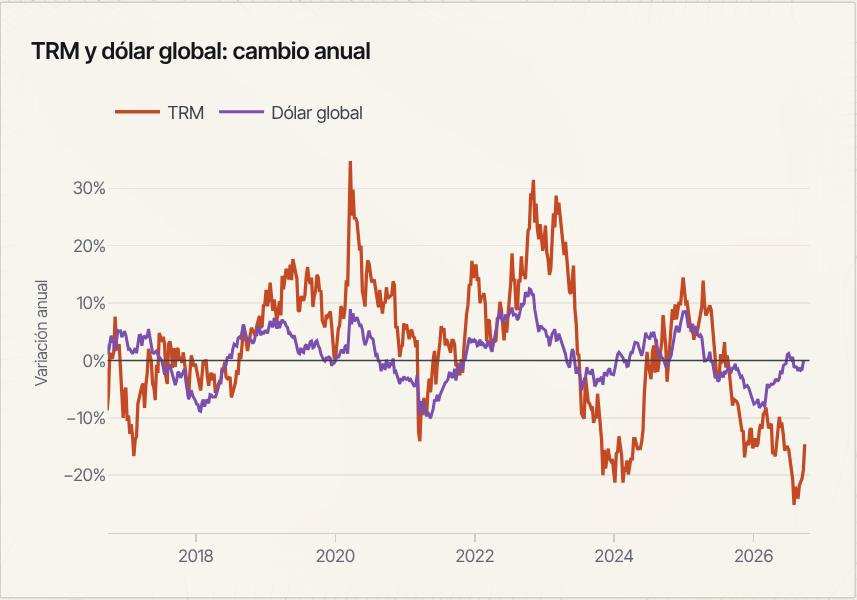
\includegraphics[width=\linewidth,height=0.42\textheight,keepaspectratio]{fig/g-tc-dolar-global.jpg}\end{center}
\paragraph{Qué nos cuenta}
Compara a lo largo del tiempo la variación anual de la TRM con la del índice amplio del dólar de la Reserva Federal, que mide el valor del dólar frente a las monedas de 26 socios comerciales de Estados Unidos. Muestra cuándo el peso ha seguido el ciclo global del dólar y cuándo se ha separado de él por razones propias.

\begin{leer}[Cómo se lee]
Dos líneas con la variación en 52 semanas, en porcentaje, usando el último dato de cada semana: naranja para la TRM (pesos por dólar) y morada para el dólar global. En ambas, positivo significa un dólar más fuerte: frente al peso en el primer caso y frente al mundo en el segundo. La línea horizontal marca el cero. El selector de horizonte cambia la ventana.
\end{leer}

\paragraph{Por qué importa}
Una buena parte de los movimientos del peso responde al ciclo financiero global, que se resume en la fortaleza del dólar. Cuando la TRM se mueve más que el dólar global, el peso amplifica los choques externos o reacciona a factores locales; separar ambos componentes ayuda a evaluar el riesgo cambiario específico de Colombia.

\paragraph{Cómo interpretarlo}
\begin{itemize}
\item Líneas juntas: el peso sigue al dólar mundial. Naranja muy por encima de la morada: el peso se debilita más de lo que explica el dólar global.
\item La TRM suele moverse con más amplitud que el índice amplio, porque este promedia monedas de economías avanzadas, menos volátiles.
\item Episodios de aversión global al riesgo tienden a llevar ambas líneas hacia arriba al mismo tiempo.
\item La correlación entre ambas cambia en el tiempo; el gráfico de correlación móvil de esta página la mide semana a semana.
\end{itemize}
\begin{formulas}[Fórmulas]
\formula{Variación de 52 semanas}{g\textsubscript{t} = (X\textsubscript{t} $\div$ X\textsubscript{t−52} − 1) $\times$ 100}{X\textsubscript{t} = TRM o índice amplio del dólar, último dato de la semana t (viernes)}
\formula{Brecha}{b\textsubscript{t} = g\textsuperscript{TRM}\textsubscript{t} − g\textsuperscript{dólar global}\textsubscript{t}}{en puntos porcentuales; positiva = el peso se debilita más que lo que se fortalece el dólar en el mundo}
\end{formulas}
\begin{metodo}[Metodología]
Variación de 52 semanas de la TRM y del índice amplio nominal del dólar (último dato de cada viernes).
\par\smallskip{\small\textbf{Fuente:} Banco de la República (TRM); Reserva Federal, H.10, vía FRED}
\end{metodo}

\section{El peso frente a otras monedas}

\subsection{Pesos por cada moneda (índice)}
\label{g:g-tc-monedas}
\begin{center}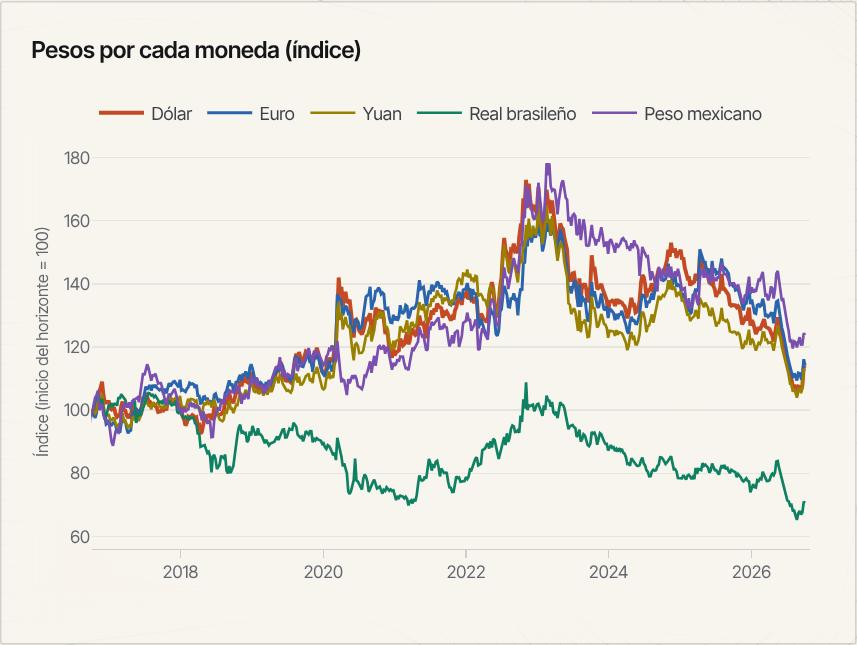
\includegraphics[width=\linewidth,height=0.42\textheight,keepaspectratio]{fig/g-tc-monedas.jpg}\end{center}
\paragraph{Qué nos cuenta}
Muestra cuántos pesos cuesta cada una de cinco monedas relevantes para Colombia (dólar, euro, yuan, real brasileño y peso mexicano), expresado como índice. Permite ver que el peso puede fortalecerse frente a una moneda y debilitarse frente a otra al mismo tiempo, según el comercio y los socios de que se trate.

\begin{leer}[Cómo se lee]
Una línea por moneda, con datos semanales (último dato de cada semana) desde 2009, re-basadas a 100 en el primer dato visible del horizonte elegido (3, 5, 10 años o todo). Naranja: dólar (TRM); azul: euro; amarilla: yuan; verde: real brasileño; morada: peso mexicano. Si una línea sube, se necesitan más pesos para comprar esa moneda: el peso se debilita frente a ella. Una línea en 120 indica 20\% más pesos por unidad que al inicio de la ventana.
\end{leer}

\paragraph{Por qué importa}
Colombia comercia con Estados Unidos, la zona euro, China y la región; el costo de las importaciones y la competitividad de las exportaciones dependen de la tasa de cambio frente a cada socio, no solo frente al dólar. Para un inversionista que mide resultados en euros u otra moneda, estas líneas muestran el efecto cambiario relevante.

\paragraph{Cómo interpretarlo}
\begin{itemize}
\item Líneas que suben juntas: el peso se debilita frente a todas, señal de un factor propio de Colombia.
\item Si la del dólar sube y las del real y el peso mexicano no, el movimiento refleja sobre todo fortaleza del dólar frente a todas las monedas de la región.
\item Los índices dependen del punto de partida: cambiar el horizonte cambia el nivel de las líneas, no su forma.
\item Real y peso mexicano se obtienen como tasas cruzadas con la TRM, por lo que heredan diferencias de fechas de corte entre fuentes.
\end{itemize}
\begin{formulas}[Fórmulas]
\formula{Tasa cruzada}{COP/X = TRM $\div$ (X por USD)}{X = real o peso mexicano; X por USD = unidades de esa moneda por dólar}
\formula{Índice re-basado}{I\textsubscript{t} = 100 $\times$ S\textsubscript{t} $\div$ S\textsubscript{0}}{S\textsubscript{t} = pesos por unidad de la moneda en la semana t; S\textsubscript{0} = valor al inicio del horizonte elegido}
\end{formulas}
\begin{metodo}[Metodología]
Pesos por unidad de cada moneda. Real y peso mexicano: tasa cruzada = TRM $\div$ (unidades de la moneda por dólar). Serie semanal; base 100 al inicio del horizonte.
\par\smallskip{\small\textbf{Fuente:} Banco de la República (tasas medias COP por EUR y CNY; TRM; real por dólar); Reserva Federal vía FRED (peso mexicano)}
\end{metodo}

\subsection{El peso frente a cada moneda: cambio en 12 meses}
\label{g:g-tc-cruces}
\begin{center}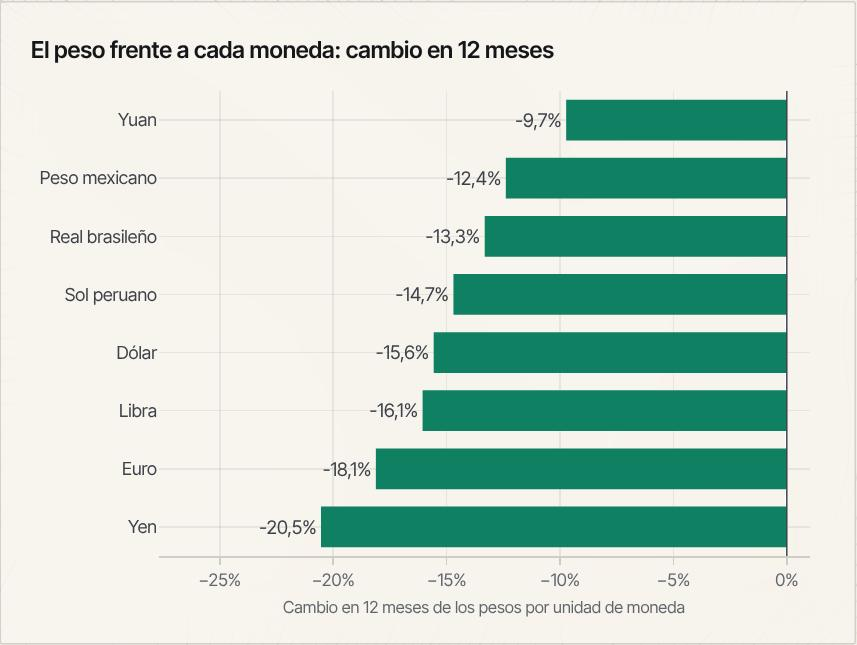
\includegraphics[width=\linewidth,height=0.42\textheight,keepaspectratio]{fig/g-tc-cruces.jpg}\end{center}
\paragraph{Qué nos cuenta}
Resume en una sola vista cuánto cambió en los últimos 12 meses el precio en pesos de ocho monedas: dólar, euro, libra esterlina, yen, yuan, real brasileño, peso mexicano y sol peruano. Muestra frente a cuáles el peso colombiano ganó o perdió valor.

\begin{leer}[Cómo se lee]
Una barra horizontal por moneda, ordenadas de la mayor caída a la mayor subida, con la variación porcentual de los pesos necesarios para comprar una unidad de esa moneda. Negativo (verde) = se necesitan menos pesos: el peso se fortaleció frente a esa moneda. Positivo (naranja) = el peso se debilitó. La línea vertical marca el cero.
\end{leer}

\paragraph{Por qué importa}
El efecto de la tasa de cambio sobre precios, exportaciones y balances depende de la moneda en que se hace cada transacción. Un peso que se fortalece frente al dólar pero se debilita frente al euro tiene efectos distintos sobre importadores de Europa y de Estados Unidos. Para inversionistas de distintas regiones, la barra de su moneda indica el efecto cambiario de los últimos 12 meses.

\paragraph{Cómo interpretarlo}
\begin{itemize}
\item Mayoría de barras verdes: el peso se fortaleció de forma generalizada; mayoría naranja, se debilitó de forma generalizada.
\item Si el peso se fortalece frente al dólar pero no frente al euro o la libra, buena parte del movimiento es debilidad global del dólar.
\item Euro, libra, yen y yuan son tasas medias que publica el Banco de la República; real, peso mexicano y sol son cruces con la TRM.
\item Son cambios nominales y de punta a punta: no recogen la volatilidad intermedia ni las diferencias de inflación.
\end{itemize}
\begin{formulas}[Fórmulas]
\formula{Variación en 12 meses}{v\textsubscript{X} = (S\textsubscript{X,t} $\div$ S\textsubscript{X,t−12m} − 1) $\times$ 100}{S\textsubscript{X} = pesos por unidad de la moneda X; t−12m = último dato disponible 12 meses antes}
\formula{Cruce con la TRM}{S\textsubscript{X} = TRM $\div$ (X por USD)}{para real, peso mexicano y sol}
\end{formulas}
\begin{metodo}[Metodología]
Variación en 12 meses de los pesos por unidad de cada moneda (tasas medias del Banco de la República; cruces con la TRM para real, peso mexicano y sol).
\par\smallskip{\small\textbf{Fuente:} Banco de la República; Reserva Federal vía FRED}
\end{metodo}

\section{Tasa de cambio real: ¿el peso está caro o barato?}

\subsection{Tasa de cambio real multilateral}
\label{g:g-tc-itcr}
\begin{center}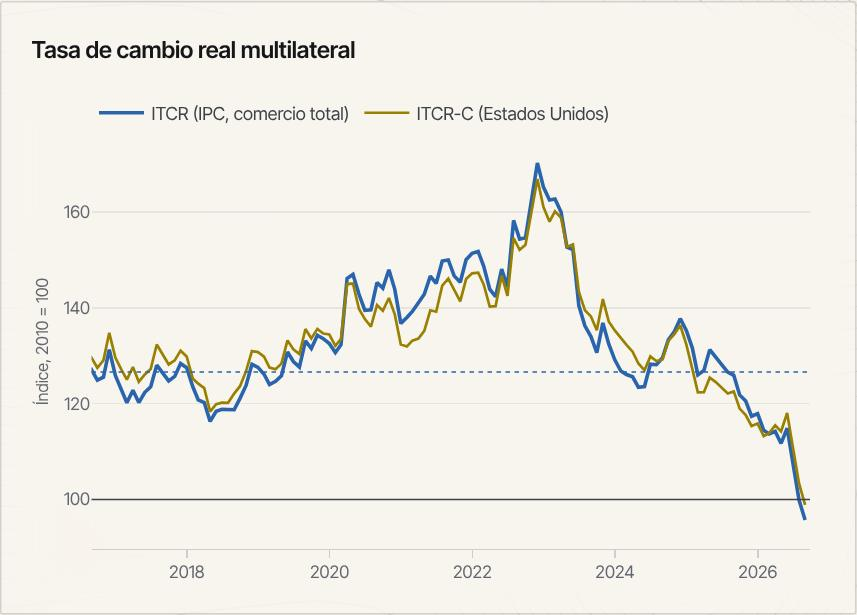
\includegraphics[width=\linewidth,height=0.42\textheight,keepaspectratio]{fig/g-tc-itcr.jpg}\end{center}
\paragraph{Qué nos cuenta}
Muestra dos medidas de la tasa de cambio real multilateral que publica el Banco de la República: el ITCR deflactado con IPC y ponderado por el comercio total con los 22 principales socios, y el ITCR-C, que mide la competitividad de Colombia frente a otros países que venden en el mercado de Estados Unidos. Ambas indican si el peso está caro o barato en términos reales.

\begin{leer}[Cómo se lee]
Líneas mensuales desde 2000, en índice con base 2010 = 100: azul para el ITCR (IPC, comercio total) y amarilla para el ITCR-C. La línea horizontal continua marca 100 y la punteada azul, el promedio del ITCR desde 2000. Cuando las líneas suben, el peso se abarata en términos reales; cuando bajan, se encarece. El selector de horizonte cambia la ventana.
\end{leer}

\paragraph{Por qué importa}
Un peso real persistentemente caro resta competitividad a exportadores e industrias que compiten con importaciones; uno barato la favorece, pero encarece insumos y bienes importados. Comparar el nivel actual con su promedio de largo plazo es una forma sencilla de ubicar la tasa de cambio real en su historia, y el ITCR-C añade la perspectiva de los exportadores que compiten en Estados Unidos.

\paragraph{Cómo interpretarlo}
\begin{itemize}
\item ITCR por encima de la línea punteada: el peso está más barato en términos reales que su promedio desde 2000; por debajo, más caro.
\item Si el ITCR-C sube más que el ITCR, Colombia gana competitividad frente a otros proveedores de Estados Unidos más de lo que gana frente al conjunto de socios.
\item El promedio histórico no es un nivel de equilibrio: cambios estructurales (por ejemplo, en los términos de intercambio) pueden desplazar el nivel de referencia.
\item Las ponderaciones son móviles de 12 meses y los índices se revisan con nuevos datos de precios y comercio.
\end{itemize}
\begin{formulas}[Fórmulas]
\formula{ITCR (esquema)}{ITCR\textsubscript{t} = $\Pi$\textsubscript{j} (E\textsubscript{j,t} $\times$ P\textsuperscript{*}\textsubscript{j,t} $\div$ P\textsubscript{t})\textsuperscript{w\textsubscript{j}}, base 2010 = 100}{E\textsubscript{j} = pesos por moneda del socio j; P\textsuperscript{*}\textsubscript{j} = IPC del socio; P = IPC de Colombia; w\textsubscript{j} = peso en el comercio total}
\formula{Promedio de referencia}{Ī = (1/T) $\times$ $\Sigma$\textsubscript{t} ITCR\textsubscript{t}}{promedio de los meses desde enero de 2000 hasta el último dato}
\formula{Distancia al promedio}{d\textsubscript{t} = (ITCR\textsubscript{t} $\div$ Ī − 1) $\times$ 100}{positiva = peso más barato que su promedio}
\end{formulas}
\begin{metodo}[Metodología]
ITCR según IPC con ponderaciones totales (22 socios) e ITCR-C (competitividad en el mercado de EE. UU.), base 2010 = 100. Línea punteada: promedio del ITCR desde 2000.
\par\smallskip{\small\textbf{Fuente:} Banco de la República}
\end{metodo}

\subsection{Tasa de cambio real bilateral frente a su promedio}
\label{g:g-tc-bilateral}
\begin{center}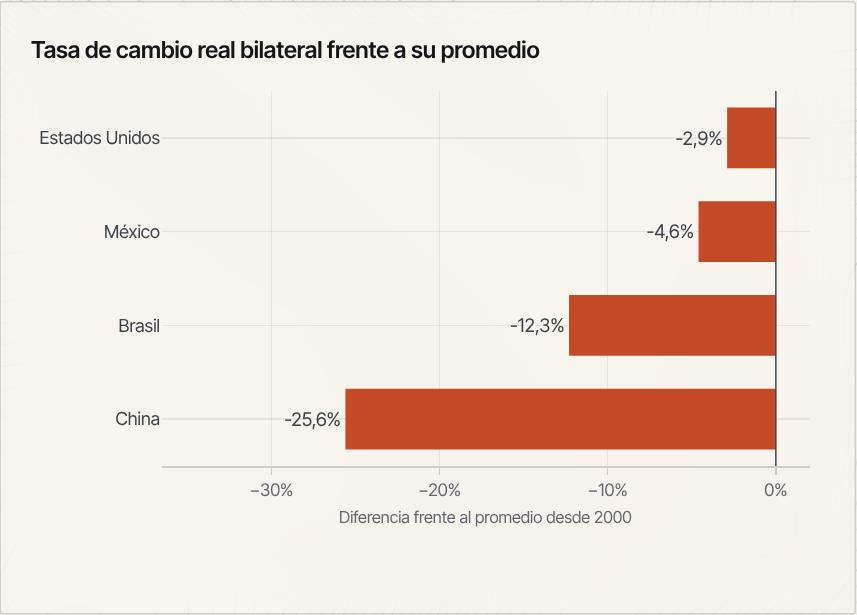
\includegraphics[width=\linewidth,height=0.42\textheight,keepaspectratio]{fig/g-tc-bilateral.jpg}\end{center}
\paragraph{Qué nos cuenta}
Muestra, para cuatro socios clave (Estados Unidos, China, Brasil y México), qué tan lejos está hoy la tasa de cambio real bilateral del peso de su promedio desde 2000. Complementa el índice multilateral al mostrar que el peso puede estar caro frente a un país y barato frente a otro.

\begin{leer}[Cómo se lee]
Una barra horizontal por país con la diferencia porcentual entre el último dato mensual del ITCR bilateral y su promedio desde 2000. Negativo (naranja) = el peso está más caro, en términos reales, que su promedio frente a ese país; positivo (azul) = más barato. La línea vertical marca el cero. Es una fotografía del último mes disponible.
\end{leer}

\paragraph{Por qué importa}
La competitividad de las exportaciones y la presión de las importaciones dependen del país: frente a Estados Unidos importa para el petróleo, el café y las flores; frente a China, para la competencia de las importaciones manufactureras; frente a Brasil y México, para el comercio regional. Un peso caro frente a un socio favorece las compras a ese país y dificulta venderle.

\paragraph{Cómo interpretarlo}
\begin{itemize}
\item Una barra de −15\% significa que el peso está 15\% más caro en términos reales que su promedio frente a ese país.
\item Diferencias grandes entre países suelen reflejar movimientos de la moneda del socio (por ejemplo, una depreciación fuerte del real) más que del peso.
\item El promedio desde 2000 es una referencia estadística, no un nivel de equilibrio.
\item Según la nota metodológica del gráfico, estos índices bilaterales se deflactan con índices de precios al productor (IPP), que reflejan mejor los precios de bienes transables.
\end{itemize}
\begin{formulas}[Fórmulas]
\formula{Distancia al promedio}{d\textsubscript{j} = (ITCR\textsubscript{j,t} $\div$ Ī\textsubscript{j} − 1) $\times$ 100}{ITCR\textsubscript{j,t} = índice bilateral con el país j en el último mes; Ī\textsubscript{j} = su promedio mensual desde enero de 2000}
\formula{ITCR bilateral (esquema)}{ITCR\textsubscript{j,t} = E\textsubscript{j,t} $\times$ P\textsuperscript{*}\textsubscript{j,t} $\div$ P\textsubscript{t}}{E\textsubscript{j} = pesos por unidad de la moneda de j; P\textsuperscript{*}\textsubscript{j}, P = índices de precios de j y de Colombia}
\end{formulas}
\begin{metodo}[Metodología]
ITCR bilateral según IPP, último mes frente a su promedio desde 2000, en porcentaje.
\par\smallskip{\small\textbf{Fuente:} Banco de la República}
\end{metodo}

\section{Petróleo y términos de intercambio}

\subsection{Petróleo y peso: cambios anuales (cada punto es un mes)}
\label{g:g-tc-brent}
\begin{center}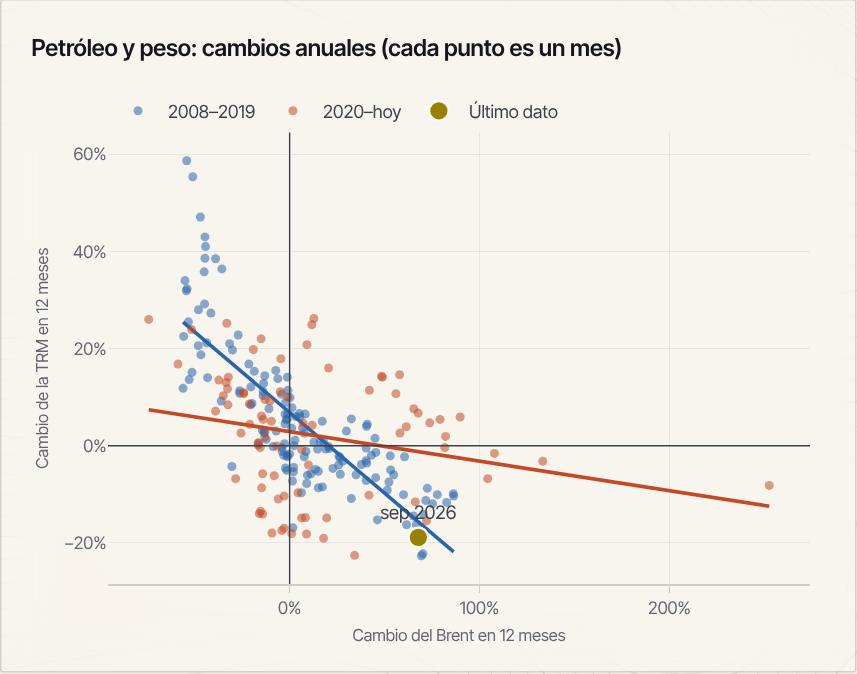
\includegraphics[width=\linewidth,height=0.42\textheight,keepaspectratio]{fig/g-tc-brent.jpg}\end{center}
\paragraph{Qué nos cuenta}
Relaciona, mes a mes, el cambio anual del precio del petróleo Brent con el cambio anual de la TRM. Como el petróleo ha sido la principal exportación de Colombia, un alza del crudo suele traer más dólares y fortalecer el peso; el gráfico muestra qué tan fuerte ha sido ese vínculo y si ha cambiado con el tiempo.

\begin{leer}[Cómo se lee]
Cada punto es un mes desde 2008. Eje horizontal: variación del Brent frente al mismo mes del año anterior; eje vertical: variación de la TRM en el mismo lapso, ambos con promedios mensuales. Azul: 2008–2019; naranja: 2020 en adelante. Cada línea es el ajuste por mínimos cuadrados de su periodo, y el punto amarillo grande, con su fecha, es el dato más reciente. Puntos abajo a la derecha = el petróleo subió y el peso se fortaleció.
\end{leer}

\paragraph{Por qué importa}
El vínculo entre petróleo y peso determina cuánto se transmiten los choques del mercado petrolero a la tasa de cambio, a la inflación y a las finanzas públicas. Un vínculo más débil indica que otros factores (flujos financieros, riesgo local, política) han ganado peso en la formación de la tasa de cambio.

\paragraph{Cómo interpretarlo}
\begin{itemize}
\item Línea con pendiente negativa: en promedio, un alza del Brent coincidió con una baja de la TRM (peso más fuerte); a mayor inclinación, más fuerte la asociación.
\item Una pendiente de −0,3 significa que un alza de 10\% del Brent en un año coincidió en promedio con una TRM 3\% más baja.
\item Puntos muy dispersos alrededor de la línea indican que el petróleo explica solo una parte de los movimientos del peso.
\item Las líneas describen la asociación observada en cada periodo; no son una relación causal ni una regla que se cumpla mes a mes.
\item Los cambios anuales de meses consecutivos se superponen en 11 meses, de modo que los puntos no son observaciones independientes.
\end{itemize}
\begin{formulas}[Fórmulas]
\formula{Cambios anuales}{x\textsubscript{m} = (B\textsubscript{m} $\div$ B\textsubscript{m−12} − 1) $\times$ 100;  y\textsubscript{m} = (T\textsubscript{m} $\div$ T\textsubscript{m−12} − 1) $\times$ 100}{B = promedio mensual del Brent; T = promedio mensual de la TRM}
\formula{Recta de mínimos cuadrados}{$\hat{y}$ = a + b $\times$ x,  b = $\Sigma$(x − $\bar{x}$)(y − $\bar{y}$) $\div$ $\Sigma$(x − $\bar{x}$)\textsuperscript{2}}{estimada por separado para 2008–2019 y para 2020 en adelante}
\formula{Correlación}{r = $\Sigma$(x − $\bar{x}$)(y − $\bar{y}$) $\div$ $\surd$[$\Sigma$(x − $\bar{x}$)\textsuperscript{2} $\times$ $\Sigma$(y − $\bar{y}$)\textsuperscript{2}]}{va de −1 a 1; mide qué tan cerca de la recta están los puntos}
\end{formulas}
\begin{metodo}[Metodología]
Promedios mensuales; variación anual de cada uno. Líneas: ajuste por mínimos cuadrados (TRM = a + b $\times$ Brent) en cada periodo; describen la asociación observada, no un pronóstico.
\par\smallskip{\small\textbf{Fuente:} EIA vía FRED (Brent); Banco de la República (TRM)}
\end{metodo}

\subsection{Correlación TRM–Brent y TRM–dólar global (52 semanas)}
\label{g:g-tc-correlacion}
\begin{center}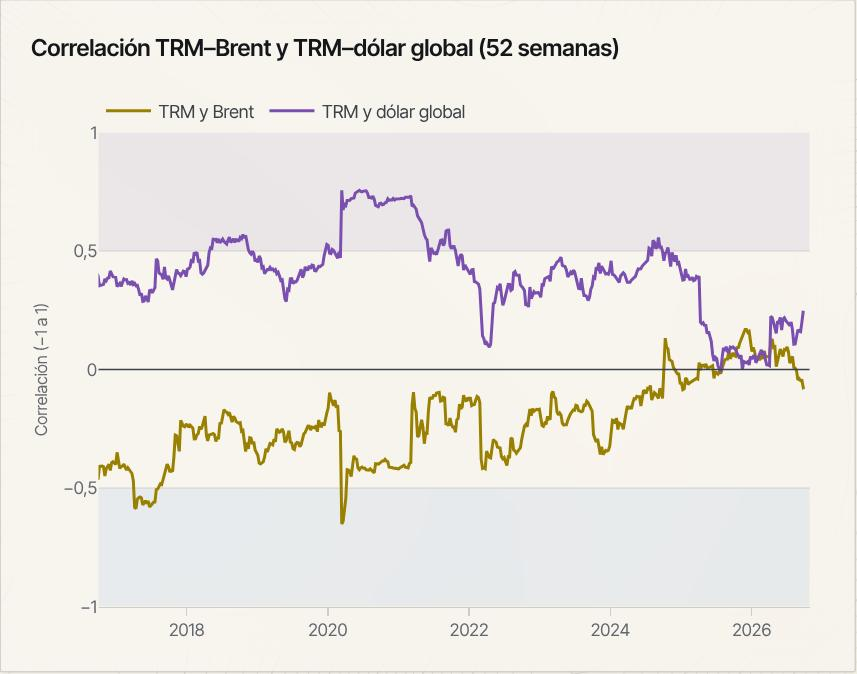
\includegraphics[width=\linewidth,height=0.42\textheight,keepaspectratio]{fig/g-tc-correlacion.jpg}\end{center}
\paragraph{Qué nos cuenta}
Muestra cómo ha cambiado en el tiempo la relación de corto plazo entre el peso y dos de sus determinantes externos: el precio del petróleo Brent y el dólar global. Para cada semana calcula la correlación de los últimos 12 meses entre los cambios semanales de la TRM y los de cada una de esas variables.

\begin{leer}[Cómo se lee]
Dos líneas semanales en una escala de −1 a 1: amarilla para la correlación TRM–Brent y morada para TRM–dólar global; la línea horizontal marca el cero. La franja azul clara (de −1 a −0,5) y la morada clara (de 0,5 a 1) señalan relaciones fuertes. Una correlación TRM–Brent cercana a −1 indica que, semana a semana, cuando el petróleo sube el peso casi siempre se fortalece; una TRM–dólar global positiva, que el peso se debilita cuando el dólar se fortalece en el mundo.
\end{leer}

\paragraph{Por qué importa}
Saber qué factor externo domina en cada momento ayuda a entender la fuente del riesgo cambiario: en unos periodos el peso responde sobre todo al petróleo, en otros al ciclo global del dólar y del apetito por riesgo. La estabilidad o inestabilidad de estas relaciones es relevante para coberturas y para evaluar la exposición de una cartera a choques externos.

\paragraph{Cómo interpretarlo}
\begin{itemize}
\item La correlación TRM–Brent suele ser negativa (petróleo arriba, peso más fuerte); cuando se acerca a cero, el petróleo pierde peso como explicación de corto plazo.
\item Una correlación TRM–dólar global dentro de la franja morada indica que el peso se mueve sobre todo con el dólar mundial.
\item Correlación no es causalidad ni magnitud: una correlación alta puede darse con movimientos pequeños; el gráfico de dispersión muestra la magnitud.
\item Con ventanas de 52 semanas, un episodio extremo puede dominar la correlación durante un año completo; se exige al menos 80\% de las semanas con dato.
\end{itemize}
\begin{formulas}[Fórmulas]
\formula{Cambio semanal}{x\textsubscript{t} = X\textsubscript{t} $\div$ X\textsubscript{t−1} − 1}{X = TRM, Brent o índice amplio del dólar, último dato de cada semana}
\formula{Correlación móvil de Pearson}{r\textsubscript{t} = $\Sigma$(x − $\bar{x}$)(y − $\bar{y}$) $\div$ $\surd$[$\Sigma$(x − $\bar{x}$)\textsuperscript{2} $\times$ $\Sigma$(y − $\bar{y}$)\textsuperscript{2}]}{sumas sobre las 52 semanas que terminan en t; x = cambio de la TRM; y = cambio del Brent o del dólar global}
\end{formulas}
\begin{metodo}[Metodología]
Correlación de Pearson móvil de 52 semanas entre variaciones semanales porcentuales.
\par\smallskip{\small\textbf{Fuente:} EIA y Reserva Federal vía FRED; Banco de la República}
\end{metodo}

\subsection{¿Cuánto pesa el petróleo en las exportaciones?}
\label{g:g-tc-petroleo-exportaciones}
\begin{center}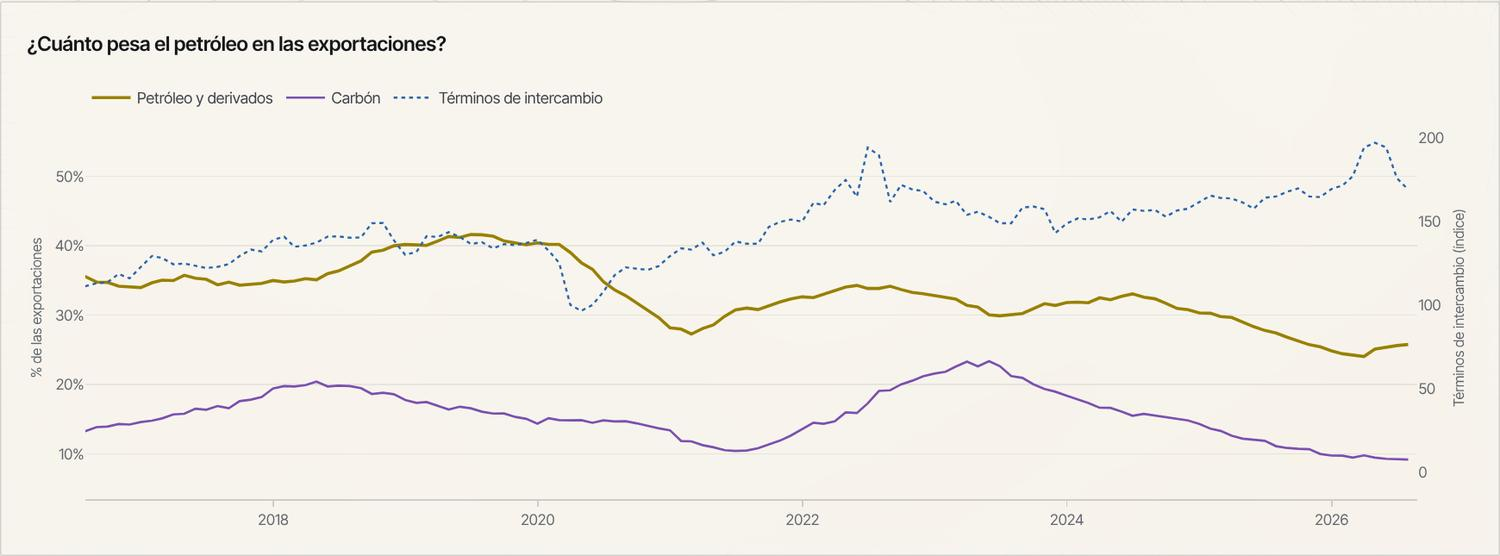
\includegraphics[width=\linewidth,height=0.42\textheight,keepaspectratio]{fig/g-tc-petroleo-exportaciones.jpg}\end{center}
\paragraph{Qué nos cuenta}
Muestra qué parte del valor de las exportaciones de bienes de Colombia corresponde al petróleo y sus derivados y al carbón, junto con los términos de intercambio, que comparan los precios de lo que el país vende con los de lo que compra. Explica por qué los precios de la energía pesan tanto en la oferta de dólares y en la tasa de cambio.

\begin{leer}[Cómo se lee]
Eje izquierdo: participación en el total exportado, en porcentaje, calculada con valores FOB en dólares sumados en 12 meses (línea amarilla, petróleo y derivados; morada, carbón). Eje derecho, línea azul punteada: índice mensual de términos de intercambio del Banco de la República. Datos desde 2000. FOB (free on board) significa valor de la mercancía puesta en el puerto de embarque, sin fletes ni seguros internacionales.
\end{leer}

\paragraph{Por qué importa}
Entre más depende el país de unas pocas materias primas, más expuestos quedan la tasa de cambio, el ingreso nacional y las finanzas públicas a sus precios internacionales. Unos términos de intercambio favorables significan que con las mismas exportaciones se pueden comprar más importaciones, lo que eleva el ingreso real del país.

\paragraph{Cómo interpretarlo}
\begin{itemize}
\item Una participación que cae puede reflejar menores precios del crudo, menor producción o un crecimiento mayor de otras exportaciones; compárela con el Brent para distinguir el efecto precio.
\item Términos de intercambio en alza indican que los precios de exportación suben más que los de importación; suelen acompañar periodos de peso más fuerte.
\item La suma de 12 meses elimina la estacionalidad y suaviza los cambios, que aparecen de forma gradual.
\item Las cifras de comercio del DANE-DIAN son provisionales en los meses más recientes y se revisan.
\end{itemize}
\begin{formulas}[Fórmulas]
\formula{Participación en las exportaciones}{s\textsubscript{t} = $\Sigma$\textsubscript{k=0}\textsuperscript{11} X\textsuperscript{p}\textsubscript{t−k} $\div$ $\Sigma$\textsubscript{k=0}\textsuperscript{11} X\textsubscript{t−k} $\times$ 100}{X\textsuperscript{p} = exportaciones FOB del producto (petróleo y derivados, o carbón) en el mes; X = exportaciones totales FOB}
\formula{Términos de intercambio}{TI\textsubscript{t} = IPX\textsubscript{t} $\div$ IPM\textsubscript{t} $\times$ 100}{IPX = índice de precios de exportación; IPM = índice de precios de importación}
\end{formulas}
\begin{metodo}[Metodología]
Exportaciones de petróleo y derivados y de carbón sobre el total, valores FOB en dólares sumados en 12 meses. Términos de intercambio: índice de precios de exportación sobre índice de precios de importación (BanRep).
\par\smallskip{\small\textbf{Fuente:} DANE-DIAN (exportaciones); Banco de la República (términos de intercambio)}
\end{metodo}

\section{¿Entran o salen dólares?}

\subsection{Balanza cambiaria: suma de 12 meses}
\label{g:g-tc-balanza}
\begin{center}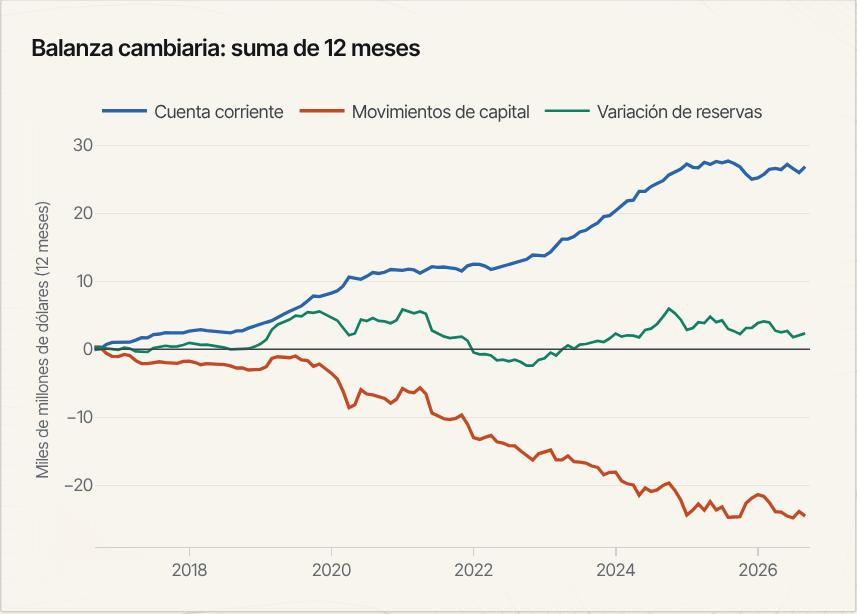
\includegraphics[width=\linewidth,height=0.42\textheight,keepaspectratio]{fig/g-tc-balanza.jpg}\end{center}
\paragraph{Qué nos cuenta}
Muestra cuántos dólares entraron o salieron de Colombia a través del mercado cambiario en los últimos 12 meses, según la balanza cambiaria del Banco de la República. Separa los flujos de comercio y transferencias (cuenta corriente) de los de inversión y financiamiento (movimientos de capital), y muestra cómo cambiaron las reservas brutas.

\begin{leer}[Cómo se lee]
Tres líneas mensuales, cada una con la suma móvil de 12 meses en miles de millones de dólares: azul para la cuenta corriente (exportaciones, importaciones, servicios y transferencias como las remesas canalizadas), naranja para los movimientos netos de capital (inversión extranjera, deuda y otros) y verde para la variación de las reservas internacionales brutas. Positivo = entran dólares; negativo = salen. La línea horizontal marca el cero.
\end{leer}

\paragraph{Por qué importa}
La oferta y la demanda de dólares del mercado cambiario son las que determinan la TRM. Un saldo de capital positivo grande puede compensar un déficit corriente; si ese financiamiento se reduce, la presión recae sobre la tasa de cambio o las reservas. Es una medida de alta frecuencia de la dependencia del país del financiamiento externo.

\paragraph{Cómo interpretarlo}
\begin{itemize}
\item Cuenta corriente negativa y capital positivo es el patrón habitual: el país compra más de lo que vende y lo financia con inversión y deuda del exterior.
\item La variación de reservas resume el balance de los flujos canalizados: positiva cuando el Banco de la República compra o acumula dólares.
\item Solo incluye operaciones canalizadas por el mercado cambiario: no es la balanza de pagos completa, que también registra operaciones que no pasan por él (por ejemplo, cuentas de compensación y reinversión de utilidades).
\item Compare con el gráfico de cuenta corriente de la página externa, que usa la balanza de pagos en porcentaje del PIB.
\end{itemize}
\begin{formulas}[Fórmulas]
\formula{Suma móvil de 12 meses}{S\textsubscript{t} = $\Sigma$\textsubscript{k=0}\textsuperscript{11} f\textsubscript{t−k} $\div$ 1.000}{f = flujo mensual en millones de dólares (cuenta corriente, capital o variación de reservas)}
\formula{Identidad aproximada}{$\Delta$Reservas $\approx$ Cuenta corriente + Capital}{en la balanza cambiaria; las diferencias provienen de otros rubros y ajustes}
\end{formulas}
\begin{metodo}[Metodología]
Balanza cambiaria mensual (operaciones canalizadas por el mercado cambiario), suma móvil de 12 meses en miles de millones de dólares.
\par\smallskip{\small\textbf{Fuente:} Banco de la República}
\end{metodo}

\subsection{Reservas internacionales netas y compras de reservas}
\label{g:g-tc-reservas}
\begin{center}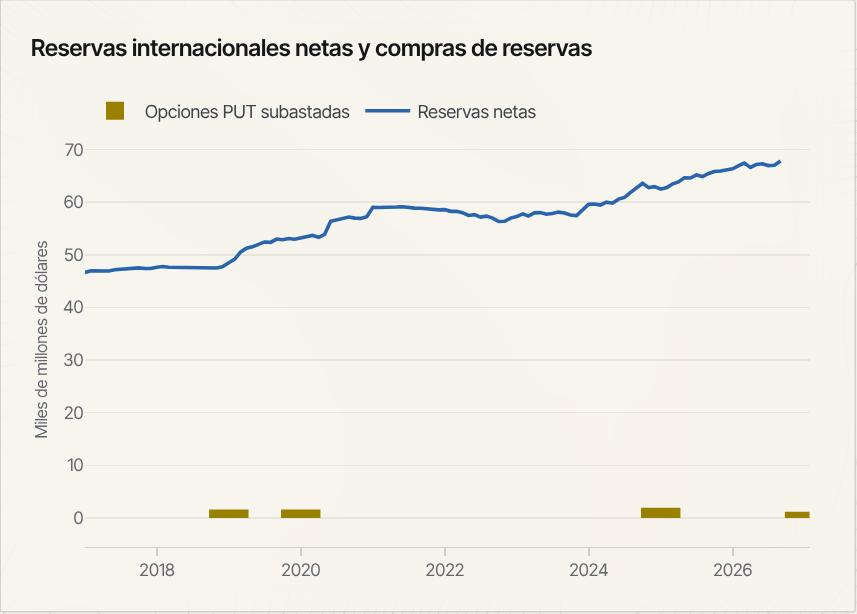
\includegraphics[width=\linewidth,height=0.42\textheight,keepaspectratio]{fig/g-tc-reservas.jpg}\end{center}
\paragraph{Qué nos cuenta}
Muestra el saldo de reservas internacionales netas del Banco de la República y los montos de opciones PUT subastadas cada año para acumularlas. Las reservas son los activos externos líquidos del banco central; las opciones PUT de acumulación son el mecanismo con el que el Banco compra dólares en el mercado de forma gradual y preanunciada.

\begin{leer}[Cómo se lee]
Línea azul: reservas internacionales netas a fin de mes, en miles de millones de dólares, desde 2000. Barras amarillas: monto aprobado en las subastas de opciones PUT para acumulación de reservas, sumado por año calendario y ubicado al final de cada año, en miles de millones de dólares. Los años sin barra son años sin subastas de acumulación.
\end{leer}

\paragraph{Por qué importa}
Las reservas son el colchón del país frente a choques externos: respaldan la capacidad de pagar importaciones y deuda en moneda extranjera y son seguidas de cerca por agencias calificadoras e inversionistas. Las compras de reservas también aumentan la demanda de dólares en el mercado, por lo que tienden a acompañar periodos en que el Banco busca fortalecer ese colchón sin fijar la tasa de cambio.

\paragraph{Cómo interpretarlo}
\begin{itemize}
\item Las reservas cambian por compras y ventas del Banco, pero también por rendimientos y por la valoración de sus inversiones y de otras monedas frente al dólar.
\item Una opción PUT da a los agentes el derecho a vender dólares al Banco; solo se ejerce si se cumplen sus condiciones, así que el monto aprobado es un tope, no la compra efectiva.
\item Para dimensionar el nivel, se suele comparar con las importaciones, la deuda externa de corto plazo o las métricas de suficiencia del FMI.
\item Compare con la línea verde del gráfico de balanza cambiaria, que muestra la variación de las reservas brutas por flujos del mercado cambiario.
\end{itemize}
\begin{formulas}[Fórmulas]
\formula{Compras anuales por opciones PUT}{P\textsubscript{a} = $\Sigma$\textsubscript{s $\in$ a} monto aprobado\textsubscript{s} $\div$ 10\textsuperscript{9}}{s = subasta de acumulación realizada en el año a; resultado en miles de millones de dólares}
\formula{Reservas netas}{RIN = reservas brutas − pasivos externos de corto plazo del Banco}{saldo a fin de mes, en miles de millones de dólares}
\end{formulas}
\begin{metodo}[Metodología]
Reservas internacionales netas (fin de mes) y monto aprobado en las subastas de opciones PUT para acumulación de reservas, sumado por año.
\par\smallskip{\small\textbf{Fuente:} Banco de la República}
\end{metodo}

\section{¿Qué tan volátil es el peso?}

\subsection{Volatilidad del peso y de sus vecinos}
\label{g:g-tc-volatilidad}
\begin{center}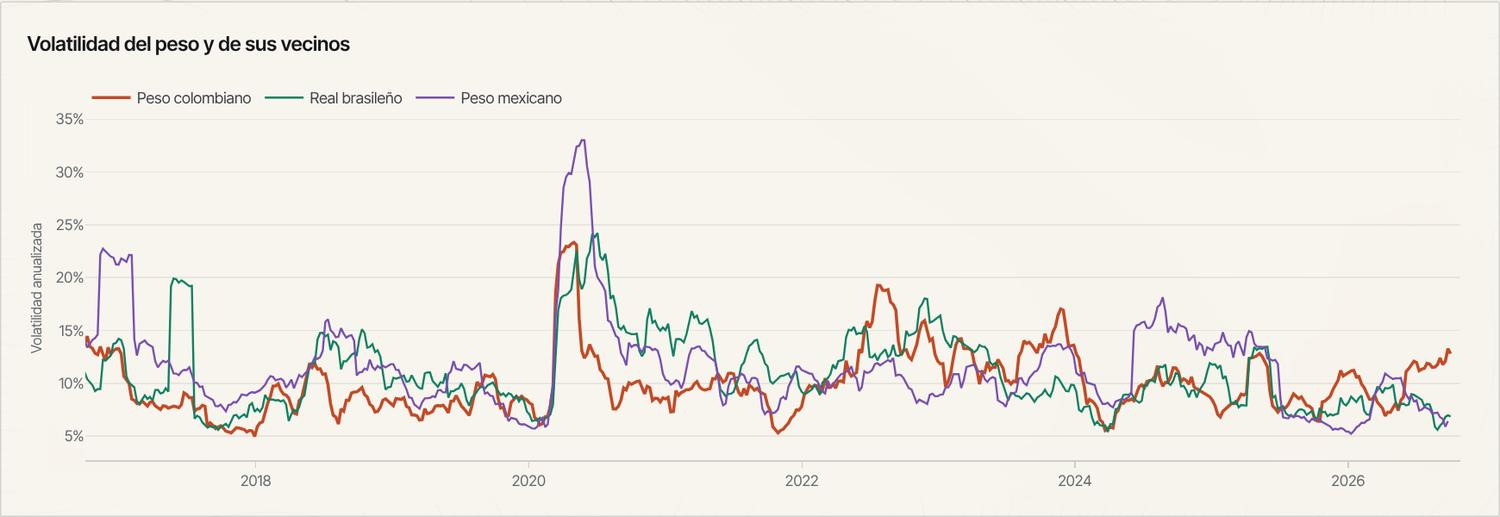
\includegraphics[width=\linewidth,height=0.42\textheight,keepaspectratio]{fig/g-tc-volatilidad.jpg}\end{center}
\paragraph{Qué nos cuenta}
Mide qué tan bruscos son los movimientos diarios del peso colombiano y los compara con los del real brasileño y el peso mexicano. La volatilidad es la desviación estándar de los cambios diarios, expresada en términos anuales; es la medida estándar del riesgo cambiario de corto plazo.

\begin{leer}[Cómo se lee]
Tres líneas desde 2008, en porcentaje anualizado, con el último dato de cada semana: naranja para el peso colombiano, verde para el real y morada para el peso mexicano. Cada punto es la desviación estándar de los cambios logarítmicos diarios en una ventana móvil de 60 observaciones, multiplicada por $\surd$252. Una volatilidad de 15\% indica que, con movimientos de esa magnitud, en un año típico la tasa varía alrededor de $\pm$15\% en una desviación estándar.
\end{leer}

\paragraph{Por qué importa}
La volatilidad cambiaria encarece las coberturas, complica la planeación de importadores, exportadores y deudores en dólares, y forma parte del riesgo que exigen los inversionistas extranjeros para entrar en activos en pesos. Compararla con la de monedas similares indica si la incertidumbre es regional o propia de Colombia.

\paragraph{Cómo interpretarlo}
\begin{itemize}
\item Picos simultáneos en las tres monedas (como en la crisis financiera global o en la pandemia de 2020) indican choques globales; un pico solo en el peso colombiano, factores locales.
\item La volatilidad mide la magnitud de los movimientos, no su dirección: puede subir tanto en depreciaciones como en apreciaciones rápidas.
\item La TRM y la tasa del real se publican todos los días del calendario, repitiendo el valor en fines de semana y festivos, mientras que el peso mexicano de la Reserva Federal solo tiene días hábiles; por eso la ventana de 60 datos abarca periodos distintos y los niveles no son estrictamente comparables entre monedas.
\item Una ventana de 60 datos reacciona rápido a los episodios de estrés pero también es ruidosa.
\end{itemize}
\begin{formulas}[Fórmulas]
\formula{Cambio logarítmico diario}{r\textsubscript{d} = ln(S\textsubscript{d} $\div$ S\textsubscript{d−1})}{S = unidades de moneda local por dólar en la observación d}
\formula{Volatilidad anualizada}{$\sigma$\textsubscript{t} = $\surd$[(1/(n−1)) $\times$ $\Sigma$\textsubscript{d} (r\textsubscript{d} − $\bar{r}$)\textsuperscript{2}] $\times$ $\surd$252 $\times$ 100}{suma sobre las últimas n = 60 observaciones (se exige al menos 48)}
\end{formulas}
\begin{metodo}[Metodología]
Desviación estándar móvil de 60 días hábiles de los cambios logarítmicos diarios, $\times$ $\surd$252.
\par\smallskip{\small\textbf{Fuente:} Banco de la República (TRM, real); Reserva Federal vía FRED (peso mexicano)}
\end{metodo}

\section*{Lecturas de la página}
\begin{itemize}\small
\item \textbf{Dornbusch, R. (1976). Expectations and Exchange Rate Dynamics. Journal of Political Economy, 84(6), 1161–1176.} Por qué la tasa de cambio reacciona más que otros precios ante choques monetarios.
\item \textbf{Meese, R. A. y Rogoff, K. (1983). Empirical Exchange Rate Models of the Seventies: Do They Fit Out of Sample? Journal of International Economics, 14(1–2), 3–24.} La tasa de cambio es difícil de anticipar: por eso este tablero solo muestra datos observados.
\item \textbf{Rogoff, K. (1996). The Purchasing Power Parity Puzzle. Journal of Economic Literature, 34(2), 647–668.} La tasa de cambio real y la paridad del poder adquisitivo.
\item \textbf{Chen, Y.-C. y Rogoff, K. (2003). Commodity Currencies. Journal of International Economics, 60(1), 133–160.} Monedas de países exportadores de materias primas y su vínculo con esos precios.
\item \textbf{Rey, H. (2013). Dilemma not Trilemma: The Global Financial Cycle and Monetary Policy Independence. Jackson Hole Economic Symposium, Federal Reserve Bank of Kansas City.} El dólar y el ciclo financiero global mueven a las monedas emergentes.
\item \textbf{Banco de la República. Metodología de cálculo del Índice de Tasa de Cambio Real (ITCR) de Colombia.} Definición del ITCR, deflactores, ponderaciones y socios comerciales.
\item \textbf{Superintendencia Financiera de Colombia. Tasa de cambio representativa del mercado: antecedentes normativos y metodología.} Cómo se calcula y certifica la TRM.
\end{itemize}

\chapter{Sector empresarial}
\label{atlas:empresas}

{\large\sffamily\bfseries Las empresas de Colombia\par}\medskip

Tamaño, rentabilidad, endeudamiento y concentración de las 10.000 empresas más grandes, sus sectores y regiones, la bolsa, el crédito a empresas y cuántas empresas nacen y cierran.

{\small\color{cmmuted}Página del sitio: \url{https://stv-quant.github.io/ColombiaMacro-USBCali/empresas/}}

\section{¿Qué empresas mueven la bolsa?}

\subsection{Bolsa de Colombia (COLCAP)}
\label{g:g-bolsa}
\begin{center}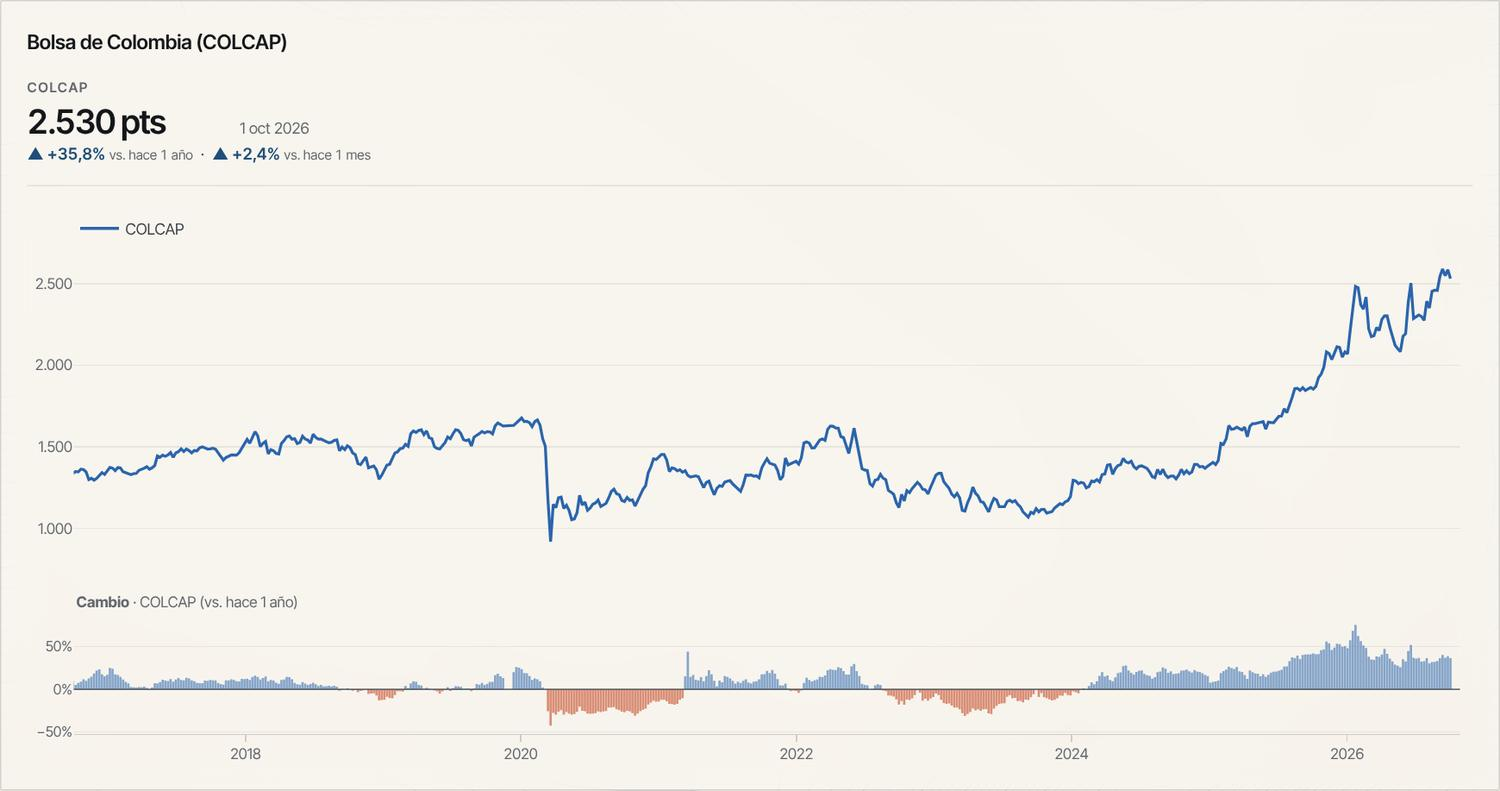
\includegraphics[width=\linewidth,height=0.42\textheight,keepaspectratio]{fig/g-bolsa.jpg}\end{center}
\paragraph{Qué nos cuenta}
Muestra la evolución del COLCAP, el índice de referencia de la Bolsa de Valores de Colombia (BVC), que resume el precio de las acciones más negociadas del país ponderadas por su valor de mercado. Es un termómetro del apetito de los inversionistas por las empresas colombianas listadas y de cómo el mercado valora sus utilidades presentes y futuras. Al no incluir dividendos, mide solo la ganancia o pérdida de precio.

\begin{leer}[Cómo se lee]
Panel superior: el nivel del COLCAP en puntos, con el último cierre de cada semana; el índice arrancó en enero de 2008 alrededor de 1.000 puntos. Panel inferior: barras con la variación porcentual frente a la misma semana un año antes, azules cuando el índice sube y naranjas cuando baja. La vista inicial abarca diez años y el selector de horizonte (3, 5, 10 años o todo) cambia la ventana; el recuadro flotante muestra el último dato y sus cambios.
\end{leer}

\paragraph{Por qué importa}
La bolsa refleja en tiempo casi real la confianza en las grandes empresas del país, buena parte de ellas bancos, petroleras y empresas de energía. Su desempeño influye en el costo del capital, en la riqueza de fondos de pensiones e inversionistas y en la percepción externa del riesgo Colombia. Para un inversionista extranjero, el rendimiento en dólares depende además de la tasa de cambio.

\paragraph{Cómo interpretarlo}
\begin{itemize}
\item Una variación anual positiva indica que el índice vale más que hace un año en pesos; comparar con la inflación muestra si hubo ganancia real.
\item El COLCAP no incluye dividendos: el rendimiento total para el accionista es mayor que el que muestra la línea, sobre todo en empresas que reparten mucho.
\item Como pondera por capitalización, unas pocas empresas grandes dominan su movimiento; el gráfico equiponderado y el de pesos de esta página muestran cuánto.
\item Para un inversionista en dólares, combine este gráfico con el de la TRM: si el peso se debilita, el rendimiento en dólares es menor que el que se ve en pesos.
\item Caídas generales del mercado, como el desplome de 2020 por la pandemia, se ven como barras naranjas profundas y simultáneas en muchas bolsas emergentes.
\end{itemize}
\begin{formulas}[Fórmulas]
\formula{Variación anual}{g\textsubscript{t} = (P\textsubscript{t} $\div$ P\textsubscript{t−52} − 1) $\times$ 100}{P\textsubscript{t} = último cierre del COLCAP en la semana t; t−52 = misma semana un año antes}
\formula{Índice de capitalización (esquema)}{I\textsubscript{t} = $\Sigma$\textsubscript{i} p\textsubscript{i,t} $\times$ q\textsubscript{i} $\div$ D\textsubscript{t}}{p = precio de la acción i; q = acciones en circulación ajustadas; D = divisor que mantiene la continuidad del índice}
\end{formulas}
\begin{metodo}[Metodología]
Índice de capitalización de las acciones más líquidas, sin dividendos; cierre semanal.
\par\smallskip{\small\textbf{Fuente:} Bolsa de Valores de Colombia (BVC), índice COLCAP, publicado por el Banco de la República}
\end{metodo}

\subsection{COLCAP, equiponderado y 7 Magníficas (base 100)}
\label{g:g-indices}
\begin{center}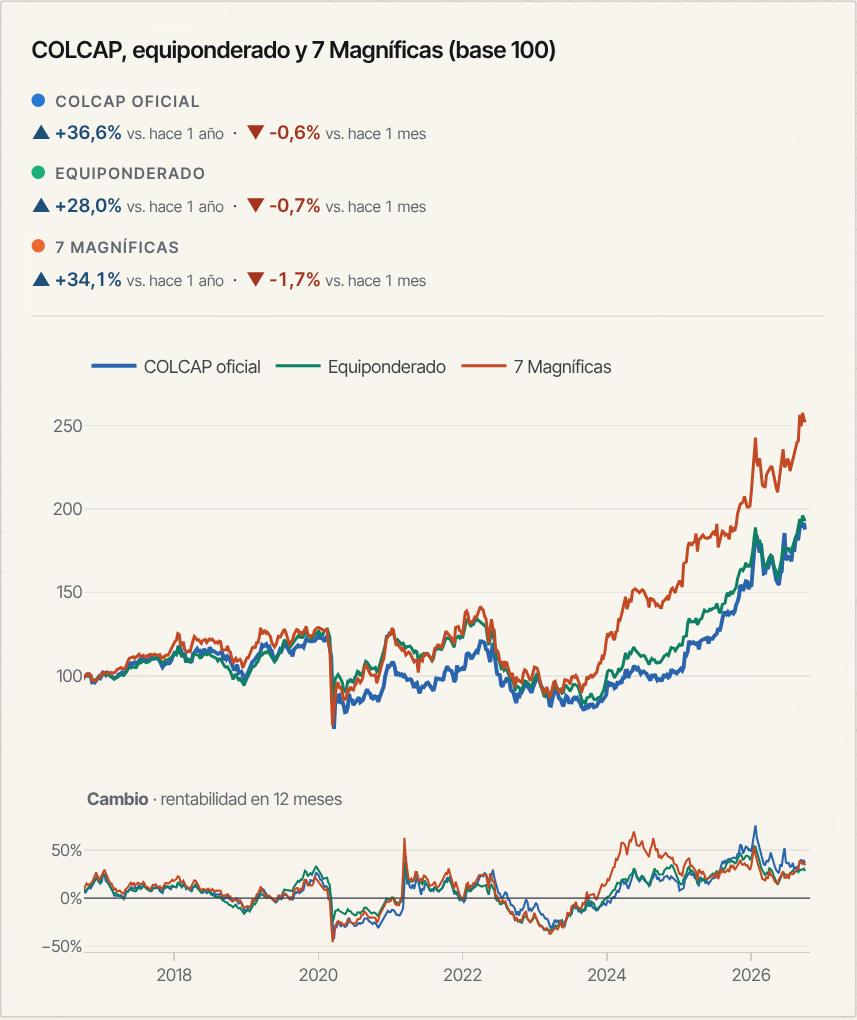
\includegraphics[width=\linewidth,height=0.42\textheight,keepaspectratio]{fig/g-indices.jpg}\end{center}
\paragraph{Qué nos cuenta}
Compara tres maneras de medir la bolsa colombiana: el COLCAP oficial, donde las empresas grandes pesan más; un índice equiponderado, donde todas las acciones de la canasta pesan lo mismo; y un índice de las 7 Magníficas, las siete empresas de mayor peso en el COLCAP, también con igual peso. La distancia entre las líneas revela si el mercado lo mueven unas pocas compañías o la mayoría de ellas.

\begin{leer}[Cómo se lee]
Panel superior: las tres series en base 100, re-basadas al primer dato visible del horizonte elegido (3, 5, 10 años o todo); azul es el COLCAP oficial, verde el equiponderado y naranja las 7 Magníficas. Una línea en 130 significa que ese índice subió 30\% desde el inicio de la ventana. Panel inferior: líneas con la rentabilidad de 12 meses de cada índice, con los mismos colores, y una línea de referencia en cero. Datos semanales.
\end{leer}

\paragraph{Por qué importa}
Un índice dominado por pocas empresas expone al inversionista a sus riesgos particulares (petróleo, banca, energía) más que a la economía en general. Si el COLCAP sube más que el equiponderado, el avance se concentra en las grandes; si ocurre lo contrario, la mejora es más amplia. Esto ayuda a entender la amplitud del mercado y la diversificación real que ofrece la bolsa local.

\paragraph{Cómo interpretarlo}
\begin{itemize}
\item COLCAP por encima del equiponderado: las acciones de mayor peso rindieron más que la acción típica; por debajo, rindieron menos.
\item Las 7 Magníficas se recalculan con cada canasta vigente; su línea muestra cómo habrían rendido las líderes de hoy, no las de cada momento.
\item El equiponderado se rebalancea cada semana (cada acción vuelve a pesar lo mismo), lo que no equivale a una cartera que se pueda replicar sin costos.
\item Sesgo de supervivencia: se usa la canasta actual hacia atrás, de modo que se omiten empresas que salieron del índice, a menudo por mal desempeño.
\item Ninguna de las tres series incluye dividendos; se descartan retornos semanales de más de $\pm$60\% por ser errores de precio de la fuente.
\end{itemize}
\begin{formulas}[Fórmulas]
\formula{Retorno semanal de cada acción}{r\textsubscript{i,t} = P\textsubscript{i,t} $\div$ P\textsubscript{i,t−1} − 1}{P\textsubscript{i,t} = cierre de la acción i en la semana t; se descarta si |r| > 0,60}
\formula{Índice equiponderado}{E\textsubscript{t} = E\textsubscript{t−1} $\times$ (1 + (1/N\textsubscript{t}) $\times$ $\Sigma$\textsubscript{i} r\textsubscript{i,t})}{N\textsubscript{t} = número de acciones con retorno válido en la semana t; para las 7 Magníficas solo se usan sus siete acciones}
\formula{Re-base al horizonte}{B\textsubscript{t} = 100 $\times$ X\textsubscript{t} $\div$ X\textsubscript{0}}{X\textsubscript{0} = valor del índice en el primer dato visible del horizonte elegido}
\formula{Rentabilidad de 12 meses}{R\textsubscript{t} = (X\textsubscript{t} $\div$ X\textsubscript{t−52} − 1) $\times$ 100}{X = nivel del índice; t−52 = misma semana un año antes}
\end{formulas}
\begin{metodo}[Metodología]
Equiponderado y 7 Magníficas: promedio simple de retornos semanales de sus acciones (rebalanceo semanal), sin dividendos; se descartan retornos semanales mayores a $\pm$60\%. Base 100 al inicio del periodo elegido. Usa la canasta actual hacia atrás (sesgo de supervivencia).
\par\smallskip{\small\textbf{Fuente:} BVC/Banco de la República (COLCAP); Yahoo Finance (precios); iShares MSCI COLCAP (canasta)}
\end{metodo}

\subsection{Cuánto pesa cada acción en el COLCAP (29 sep 2026)}
\label{g:g-pesos}
\begin{center}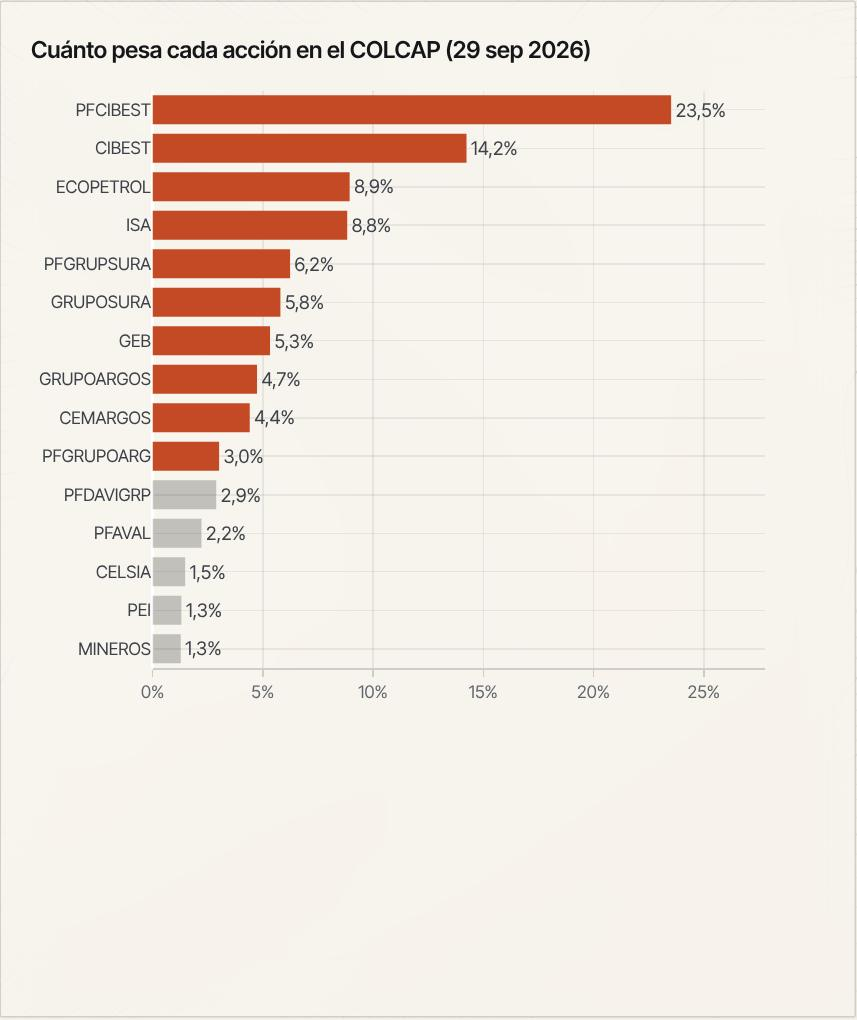
\includegraphics[width=\linewidth,height=0.42\textheight,keepaspectratio]{fig/g-pesos.jpg}\end{center}
\paragraph{Qué nos cuenta}
Muestra cuánto pesa cada una de las 15 acciones más grandes dentro del COLCAP, según la composición diaria del fondo iShares MSCI COLCAP, que replica el índice. Permite ver de un vistazo qué tan concentrada está la bolsa colombiana y qué compañías determinan la mayor parte de su movimiento.

\begin{leer}[Cómo se lee]
Barras horizontales ordenadas de mayor a menor, una por acción (identificada por su código bursátil o ticker), con su peso en porcentaje del fondo. Las barras naranjas son las acciones de las 7 Magníficas, las siete empresas de mayor peso (si una empresa tiene acción ordinaria y preferencial, ambas barras aparecen en naranja y sus pesos se suman para elegir a las siete); las grises son las demás. Al pasar el cursor se ven el nombre de la empresa y su sector. La fecha del título es la de la canasta.
\end{leer}

\paragraph{Por qué importa}
El peso de una acción indica cuánto mueve al índice: si una acción pesa 20\%, una caída de 10\% en su precio resta cerca de 2\% al COLCAP por sí sola. Para quien invierte a través de fondos que replican el índice, estos pesos son su exposición real a cada empresa y sector. Una canasta concentrada reduce la diversificación.

\paragraph{Cómo interpretarlo}
\begin{itemize}
\item La suma de las barras naranjas muestra qué parte del índice depende de siete empresas; una cifra alta indica un mercado estrecho.
\item Los pesos cambian todos los días con los precios: una acción que sube gana peso aunque no cambie la metodología.
\item Son los pesos del fondo (solo acciones, sin el efectivo), que aproximan pero no son idénticos a los oficiales de la BVC; por eso pueden no sumar exactamente 100\%.
\item Compare con el gráfico de sectores del COLCAP: la concentración por empresa suele traducirse en concentración en servicios financieros y energía.
\end{itemize}
\begin{formulas}[Fórmulas]
\formula{Peso de una acción}{w\textsubscript{i} = V\textsubscript{i} $\div$ $\Sigma$\textsubscript{j} V\textsubscript{j} $\times$ 100}{V\textsubscript{i} = valor de mercado de la posición del fondo en la acción i; $\Sigma$ sobre todo el fondo}
\formula{Peso de una empresa (para elegir las 7)}{W\textsubscript{e} = $\Sigma$\textsubscript{i $\in$ e} w\textsubscript{i}}{suma de los pesos de las clases de acción (ordinaria y preferencial) de la empresa e}
\formula{Aporte aproximado al índice}{$\Delta$I $\approx$ w\textsubscript{i} $\times$ r\textsubscript{i}}{r\textsubscript{i} = variación del precio de la acción i; $\Delta$I = efecto sobre el índice}
\end{formulas}
\begin{metodo}[Metodología]
Peso de cada acción en el fondo que replica el COLCAP (sin efectivo). Aproxima los pesos oficiales de la BVC.
\par\smallskip{\small\textbf{Fuente:} iShares MSCI COLCAP (BlackRock), composición diaria del fondo}
\end{metodo}

\section{La bolsa por dentro: acciones y sectores}

\subsection{Cambio de cada acción del COLCAP en 12 meses}
\label{g:g-em-acciones}
\begin{center}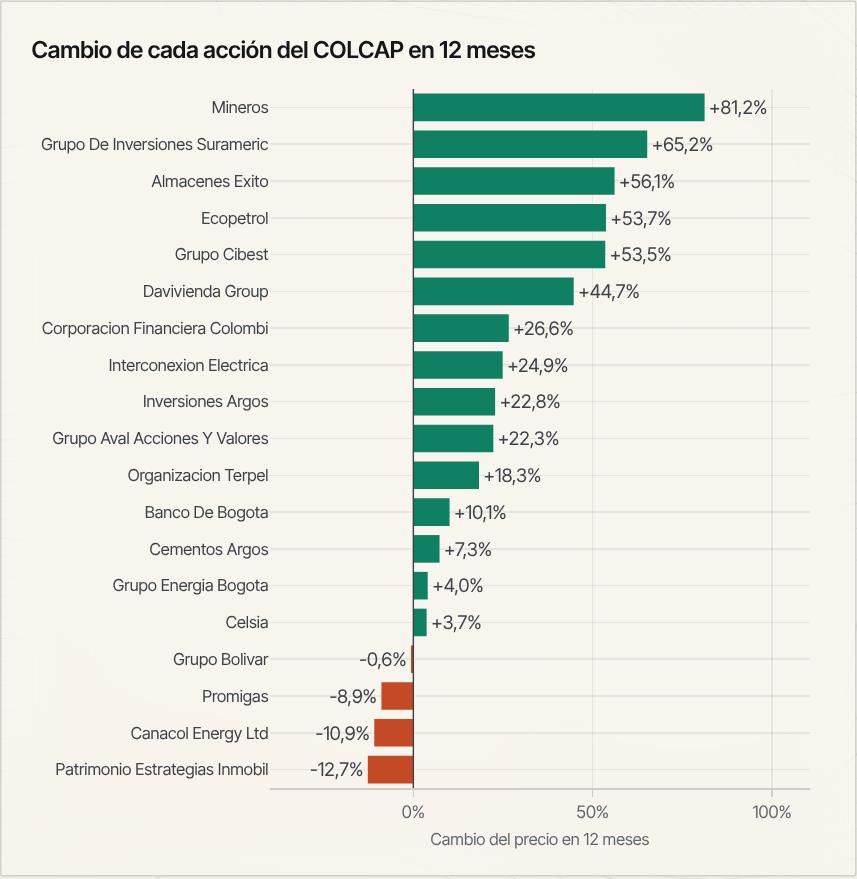
\includegraphics[width=\linewidth,height=0.42\textheight,keepaspectratio]{fig/g-em-acciones.jpg}\end{center}
\paragraph{Qué nos cuenta}
Muestra cuánto cambió en el último año el precio de cada empresa que forma parte del COLCAP. Mientras el índice resume el promedio ponderado, este gráfico revela la dispersión que hay debajo: cuántas empresas subieron, cuántas bajaron y cuáles explican el resultado del mercado.

\begin{leer}[Cómo se lee]
Una barra horizontal por empresa, ordenadas de la que más cayó a la que más subió, con la variación porcentual de su precio de cierre frente al de 52 semanas antes. Verde: el precio subió; naranja: bajó. La línea vertical marca el cero. Para empresas con varias clases de acción se usa la de mayor peso en el índice. Al pasar el cursor se ve el sector de la empresa.
\end{leer}

\paragraph{Por qué importa}
Un mercado donde suben casi todas las acciones refleja una mejora amplia de expectativas; uno donde el índice sube gracias a pocas empresas es más frágil y depende de factores específicos. Para el inversionista, la dispersión muestra el riesgo y la oportunidad de elegir acciones individuales frente a comprar el índice completo.

\paragraph{Cómo interpretarlo}
\begin{itemize}
\item Cuente las barras verdes frente a las naranjas: es una medida simple de la amplitud del mercado.
\item Una empresa con gran variación pero poco peso mueve poco el COLCAP; cruce este gráfico con el de pesos para saber cuáles importan para el índice.
\item Son variaciones de precio sin dividendos: en empresas con dividendos altos, el rendimiento total para el accionista es mayor.
\item La canasta es la vigente; una empresa recién incluida puede mostrar una variación de un periodo en que aún no estaba en el índice.
\end{itemize}
\begin{formulas}[Fórmulas]
\formula{Variación en 12 meses}{v\textsubscript{i} = (P\textsubscript{i,t} $\div$ P\textsubscript{i,t−52} − 1) $\times$ 100}{P\textsubscript{i,t} = último cierre semanal de la acción principal de la empresa i; P\textsubscript{i,t−52} = último cierre disponible 364 días o más antes}
\end{formulas}
\begin{metodo}[Metodología]
Variación del cierre semanal frente al de 52 semanas antes, sin dividendos; para empresas con varias clases de acción se usa la de mayor peso.
\par\smallskip{\small\textbf{Fuente:} Precios de cierre de las acciones de la canasta del COLCAP}
\end{metodo}

\subsection{Peso de cada sector en el COLCAP}
\label{g:g-em-colcap-sectores}
\begin{center}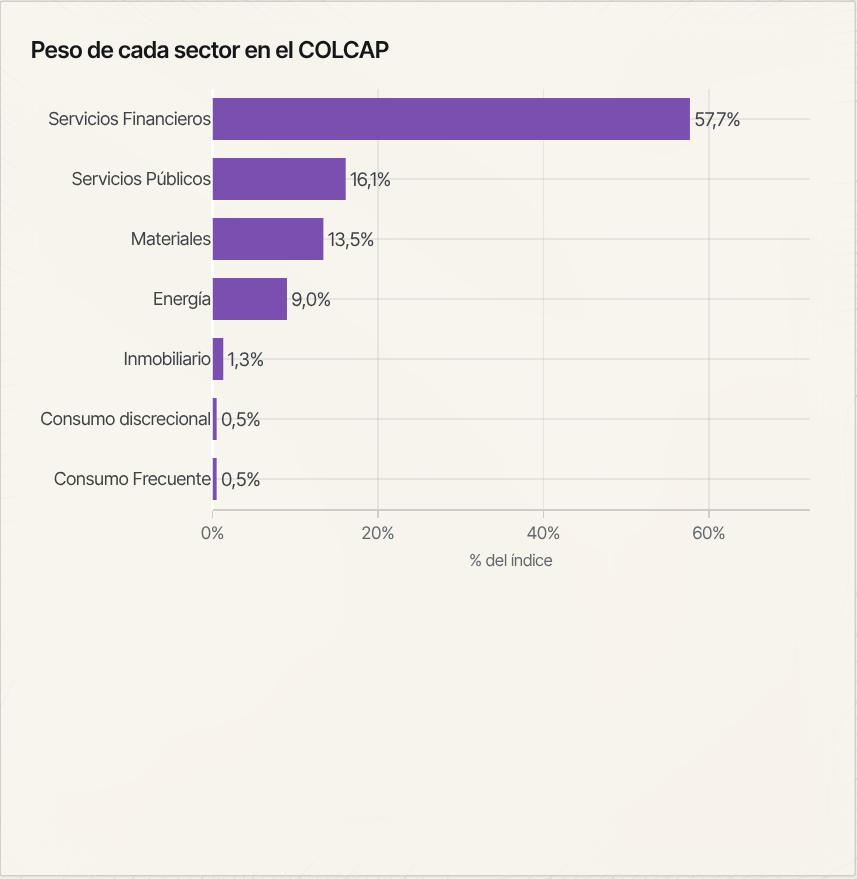
\includegraphics[width=\linewidth,height=0.42\textheight,keepaspectratio]{fig/g-em-colcap-sectores.jpg}\end{center}
\paragraph{Qué nos cuenta}
Muestra cómo se reparte el COLCAP entre sectores económicos, sumando los pesos de las acciones de cada sector en la canasta vigente. Deja ver que la bolsa colombiana no es una muestra representativa de la economía: está concentrada en pocos sectores, con un peso grande de servicios financieros y energía.

\begin{leer}[Cómo se lee]
Barras horizontales moradas, una por sector, ordenadas de menor a mayor, con el porcentaje del índice que representan sus acciones. Los sectores siguen la clasificación del proveedor del fondo iShares MSCI COLCAP (servicios financieros, energía, servicios públicos, materiales, inmobiliario y consumo, entre otros). Es una fotografía de la canasta actual, no una serie de tiempo.
\end{leer}

\paragraph{Por qué importa}
La composición sectorial determina a qué riesgos responde el índice: con mucho peso financiero y energético, el COLCAP es sensible a las tasas de interés, al crédito, al precio del petróleo y a la regulación. Para un inversionista, comprar el índice no equivale a comprar la economía colombiana, donde comercio, servicios e industria tienen un peso mucho mayor.

\paragraph{Cómo interpretarlo}
\begin{itemize}
\item Un sector con más de un tercio del índice hace que su ciclo domine el desempeño del COLCAP.
\item Compare con el gráfico de ingresos por sector de las 10.000 empresas: la bolsa sobrerrepresenta algunos sectores y casi no tiene comercio ni manufactura.
\item Los pesos se mueven con los precios: si las acciones de un sector suben más que el resto, su participación aumenta sin que cambie la canasta.
\item La clasificación sectorial es la del proveedor del fondo y puede diferir de la de la BVC o de la de Supersociedades.
\end{itemize}
\begin{formulas}[Fórmulas]
\formula{Peso de un sector}{S\textsubscript{k} = $\Sigma$\textsubscript{i $\in$ k} w\textsubscript{i}}{w\textsubscript{i} = peso (\%) de la acción i en el fondo; k = sector}
\end{formulas}
\begin{metodo}[Metodología]
Suma de pesos por sector.
\par\smallskip{\small\textbf{Fuente:} Canasta vigente del COLCAP (pesos del fondo iShares MSCI COLCAP)}
\end{metodo}

\section{Las 10.000 empresas más grandes}

\subsection{Ingresos y utilidades de las 10.000 más grandes}
\label{g:g-em-tamano}
\begin{center}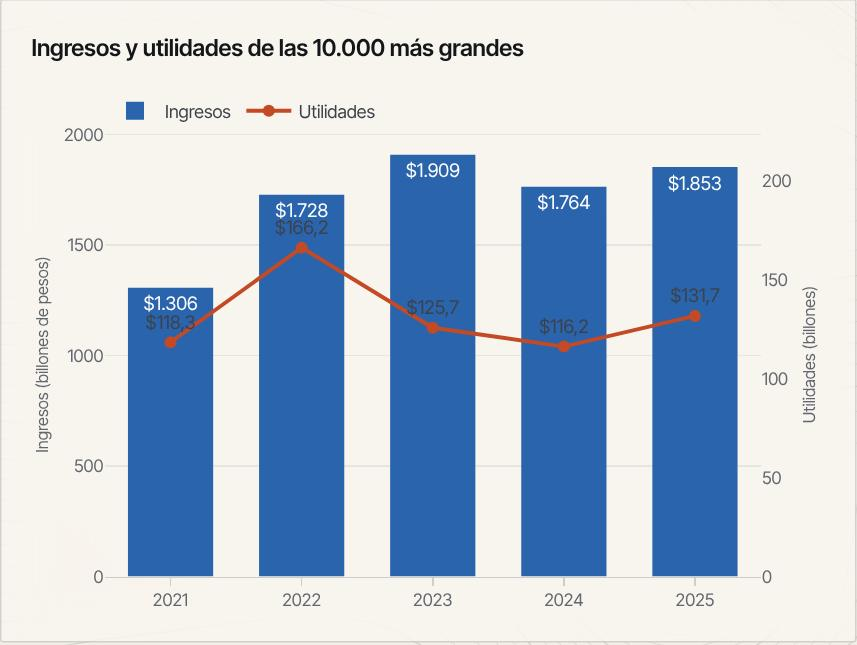
\includegraphics[width=\linewidth,height=0.42\textheight,keepaspectratio]{fig/g-em-tamano.jpg}\end{center}
\paragraph{Qué nos cuenta}
Muestra el tamaño agregado de las 10.000 empresas con más ingresos del país según la Superintendencia de Sociedades: cuánto venden (ingresos operacionales) y cuánto ganan (utilidad neta) cada año. Es la mejor aproximación disponible al pulso financiero del sector empresarial formal grande de Colombia.

\begin{leer}[Cómo se lee]
Eje horizontal: años de corte de los estados financieros (31 de diciembre). Barras azules: ingresos operacionales, en billones de pesos corrientes, eje izquierdo. Línea naranja con puntos: ganancia o pérdida neta agregada, en billones de pesos, eje derecho (que parte de cero y tiene otra escala). Las etiquetas muestran el valor de cada año.
\end{leer}

\paragraph{Por qué importa}
Los ingresos de estas empresas equivalen a una parte muy grande del PIB, de modo que su evolución refleja la demanda, los precios y la actividad del país. Las utilidades determinan la capacidad de invertir, pagar impuestos y dividendos y atender deudas. Para un inversionista, separar el crecimiento de las ventas del de las ganancias muestra si los márgenes se amplían o se estrechan.

\paragraph{Cómo interpretarlo}
\begin{itemize}
\item Son pesos corrientes: parte del crecimiento de los ingresos es inflación; restando la inflación del año se obtiene el crecimiento real.
\item La lista cambia cada año (entran y salen empresas), así que la comparación es entre las 10.000 más grandes de cada año, no entre las mismas empresas.
\item Si las utilidades crecen menos que los ingresos, el margen neto cae; el gráfico de rentabilidad lo muestra directamente.
\item Los precios del petróleo y de otras materias primas influyen mucho en el agregado por el peso de las grandes empresas mineras y energéticas.
\item Excluye bancos y aseguradoras y a las empresas que no reportan a una superintendencia.
\end{itemize}
\begin{formulas}[Fórmulas]
\formula{Ingresos agregados}{I\textsubscript{a} = $\Sigma$\textsubscript{j=1}\textsuperscript{10.000} ingresos operacionales\textsubscript{j,a}}{j = empresa de la lista del año a}
\formula{Utilidades agregadas}{G\textsubscript{a} = $\Sigma$\textsubscript{j} ganancia (pérdida)\textsubscript{j,a}}{incluye las pérdidas de las empresas con resultado negativo}
\formula{Crecimiento real de los ingresos}{c\textsuperscript{real} = (1 + c) $\div$ (1 + $\pi$) − 1}{c = variación nominal anual de I; $\pi$ = inflación promedio del año}
\end{formulas}
\begin{metodo}[Metodología]
Suma de ingresos operacionales y de ganancia (pérdida) de las 10.000 empresas de cada año, en billones de pesos corrientes.
\par\smallskip{\small\textbf{Fuente:} Superintendencia de Sociedades, 10.000 empresas más grandes (datos.gov.co)}
\end{metodo}

\subsection{Rentabilidad y endeudamiento}
\label{g:g-em-razones}
\begin{center}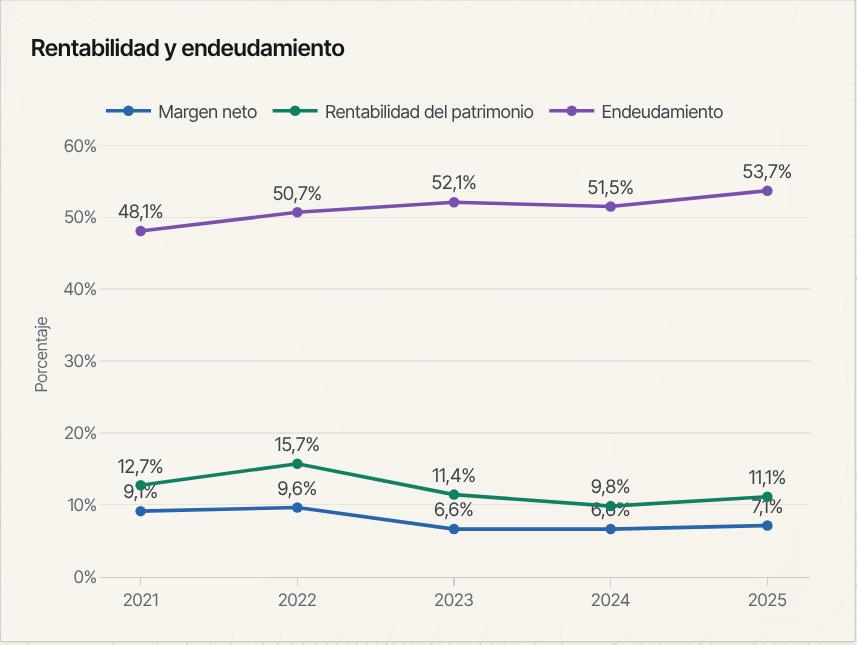
\includegraphics[width=\linewidth,height=0.42\textheight,keepaspectratio]{fig/g-em-razones.jpg}\end{center}
\paragraph{Qué nos cuenta}
Resume la salud financiera de las 10.000 empresas más grandes con tres razones calculadas sobre el agregado: el margen neto (cuánto queda de utilidad por cada peso vendido), la rentabilidad del patrimonio (lo que gana cada peso aportado por los dueños) y el endeudamiento (qué parte de los activos está financiada con deudas).

\begin{leer}[Cómo se lee]
Eje horizontal: años de corte. Eje vertical: porcentaje. Línea azul: margen neto; verde: rentabilidad del patrimonio (ROE, por su sigla en inglés); morada: endeudamiento. Cada punto lleva su valor. Las tres razones se calculan con las sumas del conjunto de empresas de cada año, no como promedio de las razones de cada empresa.
\end{leer}

\paragraph{Por qué importa}
Márgenes y rentabilidad altos indican capacidad para invertir y resistir choques; un endeudamiento creciente con rentabilidad decreciente es una combinación que eleva la fragilidad financiera, tema central en el seguimiento del Banco de la República. Para el inversionista, estas razones permiten comparar la rentabilidad empresarial con el costo del crédito y con el rendimiento de otros activos.

\paragraph{Cómo interpretarlo}
\begin{itemize}
\item Un margen neto de 7\% significa que de cada \$100 vendidos quedan \$7 de utilidad después de costos, intereses e impuestos.
\item Si la rentabilidad del patrimonio está por debajo de las tasas de interés de los bonos públicos (TES), los accionistas obtienen menos que con un activo de bajo riesgo.
\item Un endeudamiento de 60\% indica que 60 de cada 100 pesos de activos se financian con pasivos; cambios de pocos puntos son relevantes porque la razón es muy estable.
\item Al ser razones del agregado, las empresas más grandes pesan mucho; un sector con resultados extraordinarios puede mover todo el indicador.
\item La lista cambia cada año, por lo que parte de la variación se debe a qué empresas entran y salen.
\end{itemize}
\begin{formulas}[Fórmulas]
\formula{Margen neto}{M = $\Sigma$ ganancia $\div$ $\Sigma$ ingresos $\times$ 100}{sumas de las 10.000 empresas del año}
\formula{Rentabilidad del patrimonio}{ROE = $\Sigma$ ganancia $\div$ $\Sigma$ patrimonio $\times$ 100}{patrimonio = activos − pasivos, al cierre del año}
\formula{Endeudamiento}{E = $\Sigma$ pasivos $\div$ $\Sigma$ activos $\times$ 100}{proporción de los activos financiada con deudas}
\end{formulas}
\begin{metodo}[Metodología]
Razones calculadas con las sumas del agregado: ganancia/ingresos, ganancia/patrimonio y pasivos/activos.
\par\smallskip{\small\textbf{Fuente:} Superintendencia de Sociedades, 10.000 empresas más grandes (datos.gov.co)}
\end{metodo}

\section{¿En qué sectores están y cuáles ganan más?}

\subsection{Ingresos por sector (2025)}
\label{g:g-em-sectores}
\begin{center}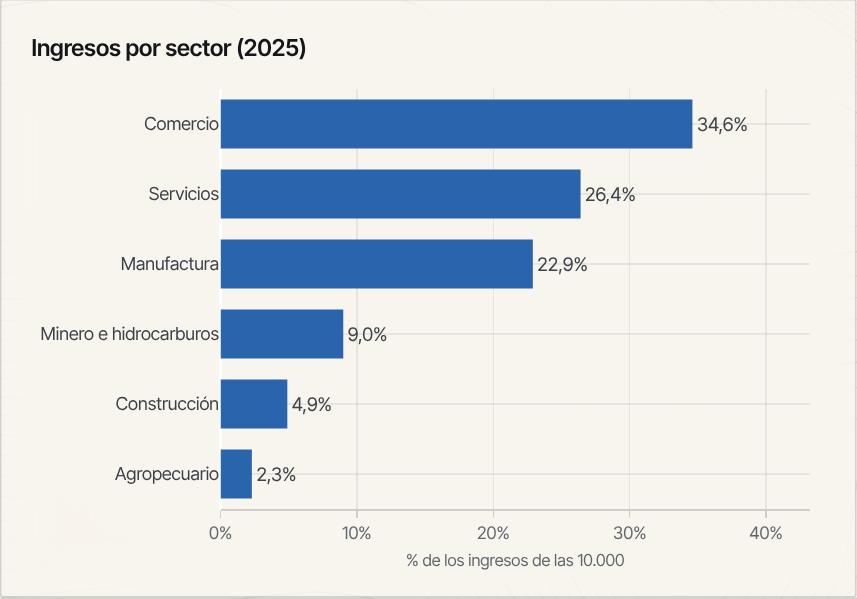
\includegraphics[width=\linewidth,height=0.42\textheight,keepaspectratio]{fig/g-em-sectores.jpg}\end{center}
\paragraph{Qué nos cuenta}
Muestra cómo se reparten los ingresos de las 10.000 empresas más grandes entre los seis macrosectores que define la Superintendencia de Sociedades: comercio, servicios, manufactura, minero e hidrocarburos, construcción y agropecuario. Indica qué actividades concentran el grueso de las ventas del sector empresarial formal grande en el último año disponible.

\begin{leer}[Cómo se lee]
Barras horizontales azules, una por macrosector, ordenadas de menor a mayor, con su participación en el total de ingresos operacionales del año (el año aparece en el título). Las participaciones suman 100\%. Al pasar el cursor se ven los ingresos del sector en billones de pesos y su variación nominal frente al año anterior.
\end{leer}

\paragraph{Por qué importa}
La estructura sectorial de los ingresos muestra de qué depende el desempeño agregado de las empresas: un peso alto del sector minero e hidrocarburos liga los resultados a los precios internacionales, mientras que comercio y servicios dependen más de la demanda interna. Para un inversionista, permite dimensionar sectores y contrastar la economía real con la composición de la bolsa.

\paragraph{Cómo interpretarlo}
\begin{itemize}
\item La participación es de ingresos, no de valor agregado: un sector con márgenes bajos y mucho volumen, como el comercio, pesa más aquí que en el PIB.
\item La variación anual del cursor es nominal e incluye el efecto de qué empresas entran y salen de la lista.
\item Compárelo con el gráfico de rentabilidad por sector: vender mucho no implica ganar mucho.
\item La clasificación es la de Supersociedades (macrosector) y no coincide exactamente con las ramas del PIB del DANE.
\end{itemize}
\begin{formulas}[Fórmulas]
\formula{Participación en los ingresos}{p\textsubscript{k} = I\textsubscript{k} $\div$ $\Sigma$\textsubscript{k} I\textsubscript{k} $\times$ 100}{I\textsubscript{k} = ingresos operacionales de las empresas del macrosector k en el año}
\formula{Variación anual (cursor)}{c\textsubscript{k} = (I\textsubscript{k,a} $\div$ I\textsubscript{k,a−1} − 1) $\times$ 100}{a = último año; a−1 = año anterior}
\end{formulas}
\begin{metodo}[Metodología]
Participación de cada macrosector de Supersociedades en los ingresos operacionales del año.
\par\smallskip{\small\textbf{Fuente:} Superintendencia de Sociedades, 10.000 empresas más grandes (datos.gov.co)}
\end{metodo}

\subsection{Rentabilidad por sector (2025)}
\label{g:g-em-sectores-rentabilidad}
\begin{center}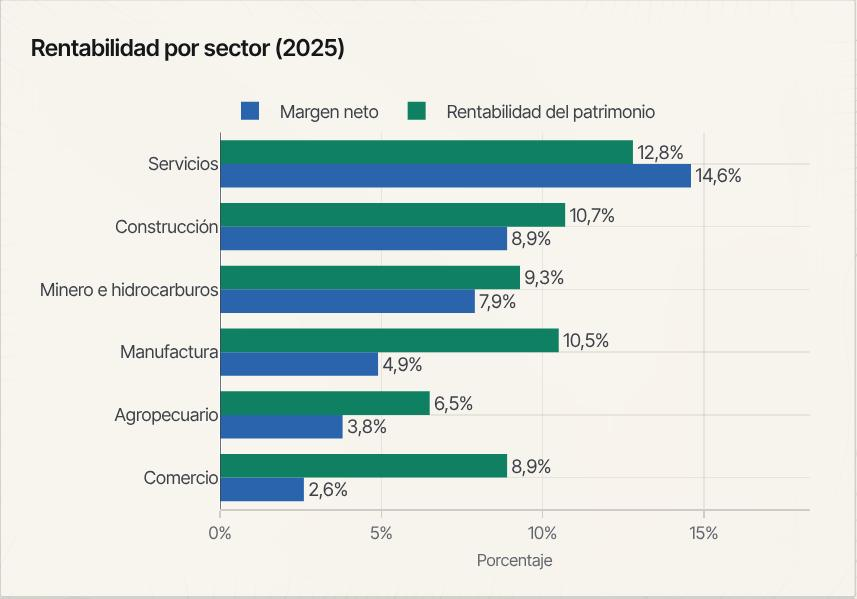
\includegraphics[width=\linewidth,height=0.42\textheight,keepaspectratio]{fig/g-em-sectores-rentabilidad.jpg}\end{center}
\paragraph{Qué nos cuenta}
Compara la rentabilidad de los seis macrosectores de Supersociedades en el último año disponible con dos medidas: el margen neto (utilidad sobre ingresos) y la rentabilidad del patrimonio (utilidad sobre patrimonio). Muestra qué actividades convierten mejor sus ventas y su capital en ganancias.

\begin{leer}[Cómo se lee]
Para cada macrosector hay dos barras horizontales: azul para el margen neto y verde para la rentabilidad del patrimonio, en porcentaje. Los sectores están ordenados por margen neto, de menor a mayor. La línea vertical marca el cero; una barra a la izquierda indica pérdidas agregadas en ese sector. El año aparece en el título.
\end{leer}

\paragraph{Por qué importa}
Las diferencias de rentabilidad entre sectores orientan la asignación de capital: los sectores más rentables atraen inversión y crédito, y los menos rentables enfrentan presión para ajustarse. Sectores como el minero suelen tener márgenes altos y volátiles, ligados a los precios internacionales, mientras que el comercio opera con márgenes estrechos y alta rotación.

\paragraph{Cómo interpretarlo}
\begin{itemize}
\item Margen bajo con rentabilidad del patrimonio alta es típico de negocios de mucho volumen y poco capital (comercio); margen alto con rentabilidad moderada, de negocios intensivos en capital.
\item Una rentabilidad del patrimonio por encima del margen indica que las ventas superan al patrimonio (alta rotación o mayor apalancamiento).
\item Son razones del agregado de cada sector: una o dos empresas muy grandes pueden determinar el resultado del sector minero o de construcción.
\item Es un solo año; la rentabilidad de sectores ligados a materias primas cambia mucho de un año a otro.
\end{itemize}
\begin{formulas}[Fórmulas]
\formula{Margen neto del sector}{M\textsubscript{k} = $\Sigma$\textsubscript{j $\in$ k} ganancia\textsubscript{j} $\div$ $\Sigma$\textsubscript{j $\in$ k} ingresos\textsubscript{j} $\times$ 100}{k = macrosector; j = empresa}
\formula{Rentabilidad del patrimonio del sector}{ROE\textsubscript{k} = $\Sigma$\textsubscript{j $\in$ k} ganancia\textsubscript{j} $\div$ $\Sigma$\textsubscript{j $\in$ k} patrimonio\textsubscript{j} $\times$ 100}{patrimonio al cierre del año}
\formula{Relación entre ambas}{ROE = M $\times$ (ingresos $\div$ patrimonio)}{la rotación del patrimonio explica la diferencia entre las dos barras}
\end{formulas}
\begin{metodo}[Metodología]
Margen neto y rentabilidad del patrimonio con las sumas de cada macrosector.
\par\smallskip{\small\textbf{Fuente:} Superintendencia de Sociedades, 10.000 empresas más grandes (datos.gov.co)}
\end{metodo}

\section{¿Dónde están las empresas?}

\subsection{Ingresos y número de empresas por región (2025)}
\label{g:g-em-regiones}
\begin{center}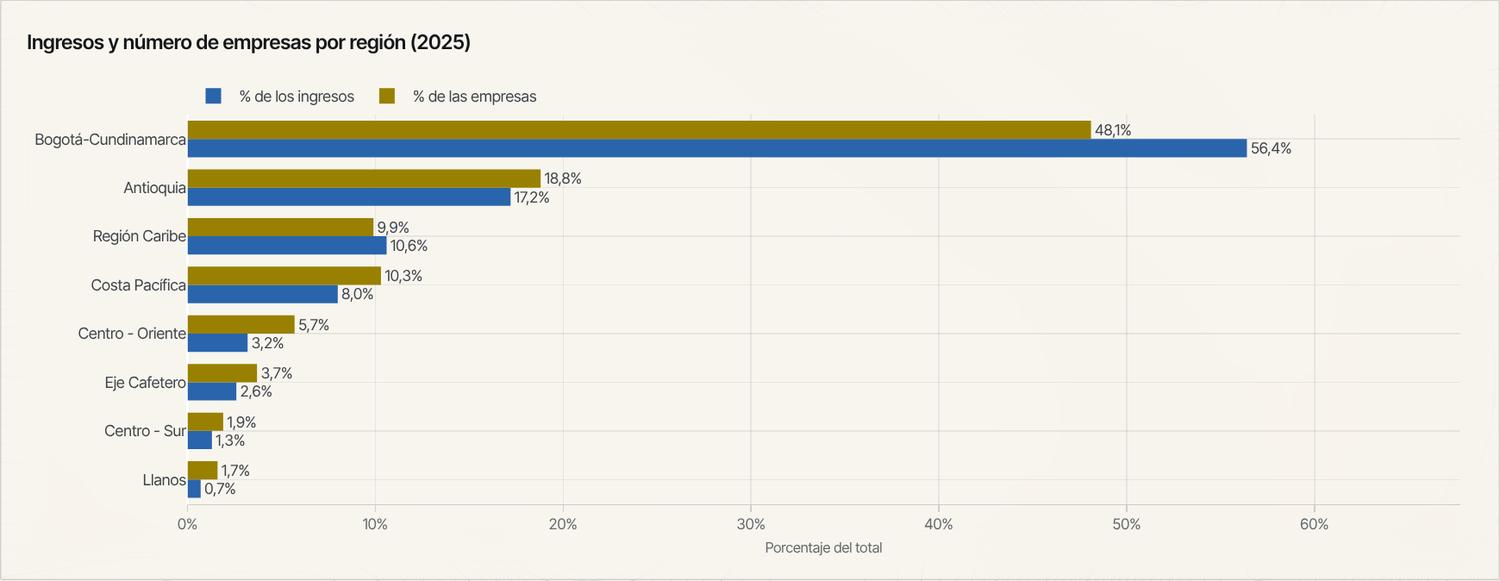
\includegraphics[width=\linewidth,height=0.42\textheight,keepaspectratio]{fig/g-em-regiones.jpg}\end{center}
\paragraph{Qué nos cuenta}
Muestra cómo se distribuyen las 10.000 empresas más grandes entre las regiones del país, tanto por sus ingresos como por el número de empresas, según el domicilio que registran ante Supersociedades. Hace visible la fuerte concentración geográfica de la actividad empresarial grande en Bogotá y Cundinamarca y en Antioquia.

\begin{leer}[Cómo se lee]
Para cada región hay dos barras horizontales: azul con su participación en los ingresos totales y amarilla con su participación en el número de empresas, ambas en porcentaje del total. Las regiones (Bogotá-Cundinamarca, Antioquia, Costa Atlántica, Región Caribe, Costa Pacífica, Eje Cafetero, Centro-Oriente, Centro-Sur, Llanos y otras) son las que define Supersociedades y están ordenadas por ingresos. El año aparece en el título.
\end{leer}

\paragraph{Por qué importa}
La concentración regional determina dónde se generan empleo formal, recaudo e inversión empresarial, y explica parte de las brechas de desarrollo entre regiones. Que una región tenga más participación en ingresos que en número de empresas indica que allí se ubican las compañías de mayor tamaño.

\paragraph{Cómo interpretarlo}
\begin{itemize}
\item Barra azul más larga que la amarilla: las empresas de esa región son, en promedio, más grandes que las del resto.
\item Las cifras se asignan al domicilio de la empresa, no a donde produce: una petrolera con sede en Bogotá suma sus ingresos a Bogotá aunque extraiga en los Llanos.
\item Por ese sesgo de sede, la concentración en la capital es mayor que la que mostraría el PIB departamental del DANE.
\item Es una sola fotografía anual; la clasificación regional es la de Supersociedades.
\end{itemize}
\begin{formulas}[Fórmulas]
\formula{Participación en ingresos}{p\textsuperscript{I}\textsubscript{r} = I\textsubscript{r} $\div$ $\Sigma$\textsubscript{r} I\textsubscript{r} $\times$ 100}{I\textsubscript{r} = ingresos de las empresas domiciliadas en la región r}
\formula{Participación en número de empresas}{p\textsuperscript{N}\textsubscript{r} = N\textsubscript{r} $\div$ 10.000 $\times$ 100}{N\textsubscript{r} = número de empresas de la región r en la lista}
\formula{Tamaño relativo}{T\textsubscript{r} = p\textsuperscript{I}\textsubscript{r} $\div$ p\textsuperscript{N}\textsubscript{r}}{mayor que 1 = empresas más grandes que el promedio}
\end{formulas}
\begin{metodo}[Metodología]
Región según el domicilio de la empresa, como la clasifica Supersociedades.
\par\smallskip{\small\textbf{Fuente:} Superintendencia de Sociedades, 10.000 empresas más grandes (datos.gov.co)}
\end{metodo}

\section{¿Qué tan concentrada está la actividad?}

\subsection{Curva de concentración de los ingresos}
\label{g:g-em-concentracion}
\begin{center}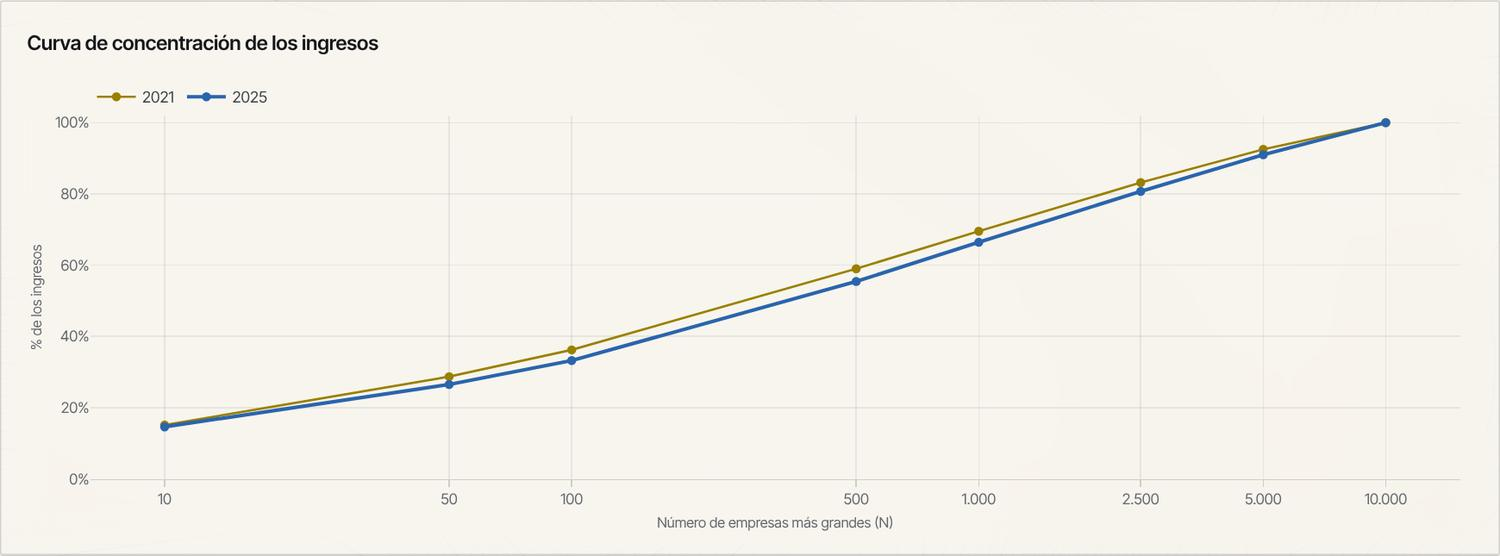
\includegraphics[width=\linewidth,height=0.42\textheight,keepaspectratio]{fig/g-em-concentracion.jpg}\end{center}
\paragraph{Qué nos cuenta}
Es una curva de concentración: muestra qué porcentaje de los ingresos de las 10.000 empresas más grandes generan las N mayores, desde las 10 primeras hasta las 10.000. Compara el primer y el último año disponibles para ver si la actividad empresarial se ha concentrado más o menos en pocas compañías.

\begin{leer}[Cómo se lee]
Eje horizontal: número de empresas más grandes (N = 10, 50, 100, 500, 1.000, 2.500, 5.000 y 10.000), en escala logarítmica para que se vean bien tanto las primeras como las últimas. Eje vertical: porcentaje acumulado de los ingresos, de 0 a 100\%. Línea azul gruesa: último año; línea amarilla delgada: primer año de la serie. Por construcción, ambas terminan en 100\% con N = 10.000.
\end{leer}

\paragraph{Por qué importa}
Una economía donde pocas empresas generan buena parte de las ventas es más sensible a los choques de esas compañías: lo que les pase se transmite al empleo, al recaudo y al crecimiento agregado (los llamados orígenes granulares de las fluctuaciones). La concentración también se relaciona con el poder de mercado y la competencia.

\paragraph{Cómo interpretarlo}
\begin{itemize}
\item Una curva más alta indica más concentración: las N mayores se quedan con una parte más grande de los ingresos.
\item Si la línea azul está por encima de la amarilla, la concentración aumentó entre el primer y el último año; si está por debajo, disminuyó.
\item Los precios del petróleo afectan esta medida: cuando suben, la mayor empresa del país gana participación y la curva sube en su tramo inicial.
\item Mide concentración dentro de las 10.000, no en toda la economía, ni por mercado o producto.
\end{itemize}
\begin{formulas}[Fórmulas]
\formula{Participación acumulada}{C\textsubscript{N} = $\Sigma$\textsubscript{j=1}\textsuperscript{N} I\textsubscript{(j)} $\div$ $\Sigma$\textsubscript{j=1}\textsuperscript{10.000} I\textsubscript{(j)} $\times$ 100}{I\textsubscript{(j)} = ingresos de la empresa que ocupa el puesto j, ordenadas de mayor a menor}
\end{formulas}
\begin{metodo}[Metodología]
Ingresos de las N empresas más grandes sobre los ingresos de las 10.000, para el primer y el último año disponibles.
\par\smallskip{\small\textbf{Fuente:} Superintendencia de Sociedades, 10.000 empresas más grandes (datos.gov.co)}
\end{metodo}

\section{¿Cómo se financian las empresas?}

\subsection{Crédito a empresas y su costo}
\label{g:g-em-credito}
\begin{center}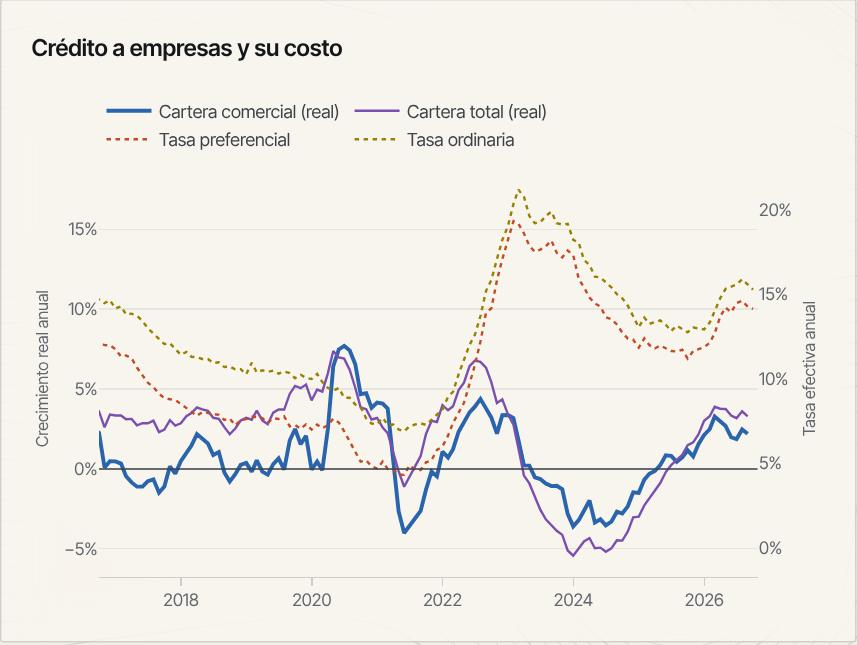
\includegraphics[width=\linewidth,height=0.42\textheight,keepaspectratio]{fig/g-em-credito.jpg}\end{center}
\paragraph{Qué nos cuenta}
Muestra cuánto crece el crédito bancario a las empresas descontada la inflación y cuánto cuesta. Compara la cartera comercial (préstamos en pesos a empresas) con la cartera total del sistema y las tasas de interés de los créditos preferencial (a grandes empresas de bajo riesgo) y ordinario. Es un indicador de cómo se transmite la política monetaria a la financiación empresarial.

\begin{leer}[Cómo se lee]
Eje izquierdo, líneas sólidas: crecimiento real anual del saldo de la cartera comercial (azul, gruesa) y de la cartera total (morada), en porcentaje; la línea horizontal marca el cero. Eje derecho, líneas punteadas: tasa del crédito preferencial o corporativo (naranja) y del ordinario (amarilla), en porcentaje efectivo anual, promedio mensual de los datos semanales. Datos mensuales desde 2008.
\end{leer}

\paragraph{Por qué importa}
El crédito financia capital de trabajo e inversión: cuando su crecimiento real cae por debajo de cero, las empresas en conjunto están reduciendo su deuda bancaria real, lo que suele acompañar fases de menor inversión. Las tasas muestran el costo de esa financiación y responden, con rezago, a la tasa de política monetaria (TPM) del Banco de la República.

\paragraph{Cómo interpretarlo}
\begin{itemize}
\item Crecimiento real negativo significa que el saldo de crédito crece menos que la inflación, aunque en pesos corrientes siga aumentando.
\item Tasas en alza con crédito desacelerándose son típicas de una política monetaria restrictiva; la combinación inversa, de una política expansiva.
\item La tasa preferencial es menor que la ordinaria porque se otorga a clientes de menor riesgo; la brecha entre ambas refleja la percepción de riesgo.
\item Compare con el gráfico de la TPM en la página de tasas: las tasas de colocación siguen a la de política con meses de rezago.
\item La cartera es en moneda legal (pesos): no incluye préstamos en dólares, bonos corporativos ni crédito de proveedores.
\end{itemize}
\begin{formulas}[Fórmulas]
\formula{Crecimiento real anual del saldo}{g\textsuperscript{real}\textsubscript{t} = [(1 + g\textsubscript{t}) $\div$ (1 + $\pi$\textsubscript{t}) − 1] $\times$ 100}{g\textsubscript{t} = S\textsubscript{t} $\div$ S\textsubscript{t−12} − 1, con S = saldo de cartera del mes t; $\pi$\textsubscript{t} = inflación anual del IPC del mes t}
\formula{Tasa mensual}{i\textsubscript{m} = (1/n) $\times$ $\Sigma$\textsubscript{s} i\textsubscript{s}}{i\textsubscript{s} = tasa efectiva anual de la semana s del mes; n = semanas con dato}
\end{formulas}
\begin{metodo}[Metodología]
Crecimiento real = (1 + variación anual del saldo)/(1 + inflación anual) − 1. Tasas: promedio mensual de datos semanales, efectiva anual.
\par\smallskip{\small\textbf{Fuente:} Banco de la República (cartera y tasas de colocación); DANE (IPC)}
\end{metodo}

\subsection{Posición financiera neta por sector (\% del PIB)}
\label{g:g-em-posicion}
\begin{center}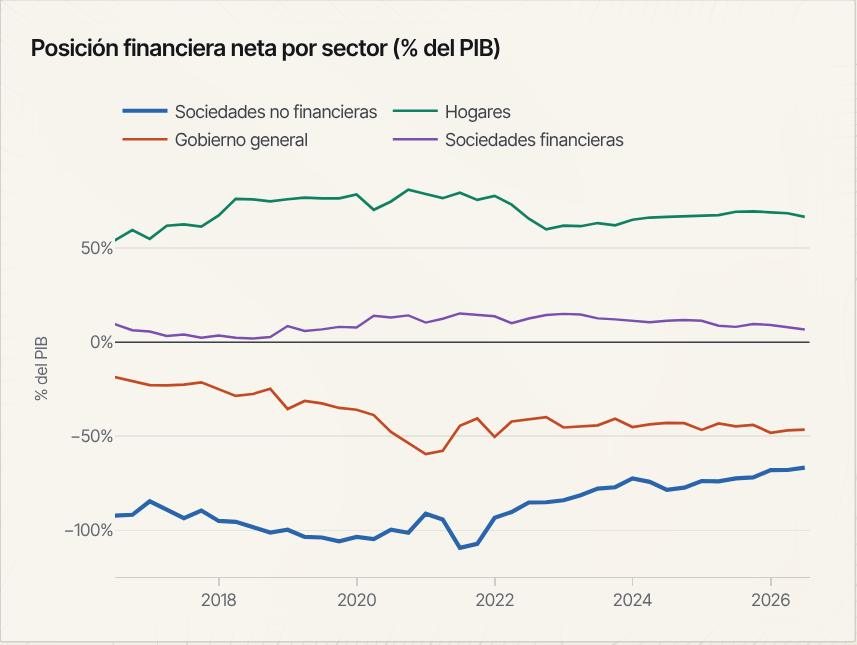
\includegraphics[width=\linewidth,height=0.42\textheight,keepaspectratio]{fig/g-em-posicion.jpg}\end{center}
\paragraph{Qué nos cuenta}
Muestra la posición financiera neta de cada sector institucional de la economía según las cuentas financieras del Banco de la República: lo que cada sector tiene en activos financieros (depósitos, bonos, acciones, préstamos otorgados) menos lo que debe. Indica qué sectores financian a los demás y cuáles se financian con el ahorro ajeno.

\begin{leer}[Cómo se lee]
Líneas trimestrales en porcentaje del PIB, desde 2015: sociedades no financieras (azul, gruesa), hogares (verde), gobierno general (naranja) y sociedades financieras (morada). La línea horizontal marca el cero: por encima, el sector es acreedor neto; por debajo, deudor neto. Los saldos de los sectores internos no suman cero, porque la diferencia corresponde a la posición frente al resto del mundo.
\end{leer}

\paragraph{Por qué importa}
Las empresas no financieras suelen ser deudoras netas porque invierten más de lo que ahorran y emiten acciones y deuda; los hogares suelen ser acreedores netos. Una posición deudora creciente de empresas o gobierno indica mayor dependencia del financiamiento de otros sectores o del exterior, lo que eleva la sensibilidad a las tasas de interés y a la tasa de cambio.

\paragraph{Cómo interpretarlo}
\begin{itemize}
\item Negativo = el sector se financia con los demás; positivo = financia a otros sectores.
\item Los pasivos de las sociedades incluyen las acciones y participaciones de capital: una posición negativa no es solo deuda.
\item Los saldos se valoran a precios de mercado, así que cambian con la tasa de cambio y con los precios de las acciones y los bonos, no solo con nuevos flujos.
\item La suma de los cuatro sectores aproxima la posición de inversión internacional (PII) del país, con signo contrario a la del resto del mundo.
\item Las cuentas financieras se publican con rezago y se revisan.
\end{itemize}
\begin{formulas}[Fórmulas]
\formula{Posición financiera neta}{PFN\textsubscript{s,t} = (A\textsubscript{s,t} − P\textsubscript{s,t}) $\div$ PIB\textsubscript{t} $\times$ 100}{A = activos financieros; P = pasivos (incluidas acciones emitidas) del sector s al final del trimestre t; PIB = PIB nominal de referencia que usa el Banco de la República}
\formula{Identidad agregada}{$\Sigma$\textsubscript{s} PFN\textsubscript{s} = − PFN\textsubscript{resto del mundo}}{los sectores internos en conjunto son acreedores o deudores del exterior}
\end{formulas}
\begin{metodo}[Metodología]
Posición neta = activos financieros − pasivos de cada sector institucional, en porcentaje del PIB, trimestral.
\par\smallskip{\small\textbf{Fuente:} Banco de la República, cuentas financieras (saldos)}
\end{metodo}

\section{¿Nacen o cierran empresas?}

\subsection{Empresas que nacen y que cierran (suma de 12 meses)}
\label{g:g-em-registro}
\begin{center}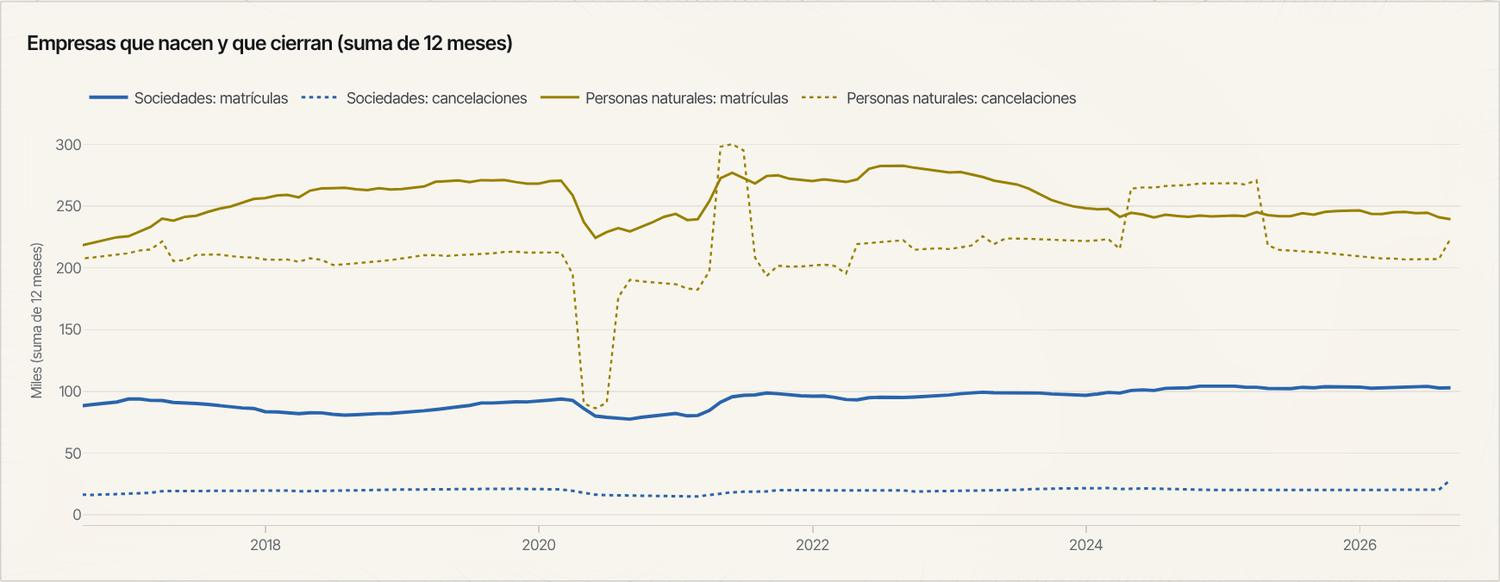
\includegraphics[width=\linewidth,height=0.42\textheight,keepaspectratio]{fig/g-em-registro.jpg}\end{center}
\paragraph{Qué nos cuenta}
Muestra cuántas empresas se crean y cuántas cierran en Colombia, a partir de las matrículas y cancelaciones en el registro mercantil que llevan las cámaras de comercio (RUES, Registro Único Empresarial y Social, administrado por Confecámaras). Distingue las sociedades de las personas naturales con negocio propio, y es una señal temprana del dinamismo empresarial.

\begin{leer}[Cómo se lee]
Cuatro líneas mensuales, cada una con la suma de los últimos 12 meses en miles, desde 2012. Azul: sociedades (personas jurídicas principales y entidades sin ánimo de lucro); amarillo: personas naturales. Línea sólida: matrículas (nacimientos); punteada: cancelaciones (cierres). Se descarta el último mes si aún está incompleto. El selector de horizonte cambia la ventana.
\end{leer}

\paragraph{Por qué importa}
La creación de empresas refleja la confianza para emprender y la demanda esperada; las cancelaciones, el cierre de negocios. La diferencia entre ambas aproxima la creación neta de unidades productivas formales, ligada al empleo formal. Para un inversionista, es una medida del dinamismo del tejido empresarial, especialmente de las pequeñas empresas que no aparecen en la bolsa ni en las 10.000 más grandes.

\paragraph{Cómo interpretarlo}
\begin{itemize}
\item Matrículas por encima de cancelaciones: el número de unidades registradas aumenta; la brecha entre la línea sólida y la punteada de un mismo color es la creación neta.
\item La suma de 12 meses suaviza la estacionalidad del calendario de registro pero hace que los cambios aparezcan de forma gradual.
\item Las cancelaciones incluyen depuraciones masivas del registro ordenadas por norma, que generan saltos que no son cierres económicos de ese momento.
\item Una matrícula no equivale a una empresa en operación ni a empleo creado; es un conteo administrativo.
\item Compare con el gráfico de crédito: periodos de crédito real débil suelen coincidir con menor creación de sociedades.
\end{itemize}
\begin{formulas}[Fórmulas]
\formula{Suma móvil de 12 meses}{S\textsubscript{t} = $\Sigma$\textsubscript{k=0}\textsuperscript{11} x\textsubscript{t−k} $\div$ 1.000}{x = matrículas o cancelaciones del mes, por fecha de matrícula o de cancelación}
\formula{Creación neta}{N\textsubscript{t} = S\textsuperscript{matrículas}\textsubscript{t} − S\textsuperscript{cancelaciones}\textsubscript{t}}{para sociedades o para personas naturales}
\formula{Mes incompleto}{se descarta el mes t si x\textsubscript{t} < 0,5 $\times$ mediana(x\textsubscript{t−12}, …, x\textsubscript{t−1})}{x = matrículas totales del mes}
\end{formulas}
\begin{metodo}[Metodología]
Conteo de matrículas por fecha de matrícula y de cancelaciones por fecha de cancelación; suma móvil de 12 meses. Se descarta el último mes si aún está incompleto.
\par\smallskip{\small\textbf{Fuente:} Confecámaras, Registro Único Empresarial y Social (datos.gov.co)}
\end{metodo}

\section*{Lecturas de la página}
\begin{itemize}\small
\item \textbf{Modigliani, F. y Miller, M. H. (1958). The Cost of Capital, Corporation Finance and the Theory of Investment. American Economic Review, 48(3), 261–297.} Cómo se relacionan endeudamiento, patrimonio y valor de la empresa.
\item \textbf{Rajan, R. G. y Zingales, L. (1998). Financial Dependence and Growth. American Economic Review, 88(3), 559–586.} Los sectores que dependen del crédito crecen más donde el sistema financiero es más profundo.
\item \textbf{Bernanke, B. S., Gertler, M. y Gilchrist, S. (1999). The Financial Accelerator in a Quantitative Business Cycle Framework. Handbook of Macroeconomics, 1C, 1341–1393.} La salud financiera de las empresas amplifica el ciclo económico.
\item \textbf{Gabaix, X. (2011). The Granular Origins of Aggregate Fluctuations. Econometrica, 79(3), 733–772.} Cuando unas pocas empresas son muy grandes, sus choques mueven a toda la economía.
\item \textbf{Hsieh, C.-T. y Klenow, P. J. (2009). Misallocation and Manufacturing TFP in China and India. Quarterly Journal of Economics, 124(4), 1403–1448.} La asignación de recursos entre empresas y la productividad agregada.
\item \textbf{Superintendencia de Sociedades. Informe de las 10.000 empresas más grandes del país (2026, cifras a diciembre de 2025).} Fuente de las cifras de tamaño, rentabilidad y endeudamiento.
\item \textbf{Banco de la República. Reporte de Estabilidad Financiera (semestral).} Seguimiento oficial de la situación financiera de las empresas y su deuda.
\end{itemize}

\chapter{Externo y fiscal}
\label{atlas:externo}

{\large\sffamily\bfseries Cuentas externas y fiscales\par}\medskip

La balanza de pagos por componentes, cómo se financia, la inversión extranjera y las remesas, la deuda externa, y los ingresos, gastos, intereses, financiamiento y deuda del Gobierno.

{\small\color{cmmuted}Página del sitio: \url{https://stv-quant.github.io/ColombiaMacro-USBCali/externo/}}

\section{¿Cómo están las cuentas con el exterior y del Gobierno?}

\subsection{Cuenta corriente (\% del PIB)}
\label{g:g-cc}
\begin{center}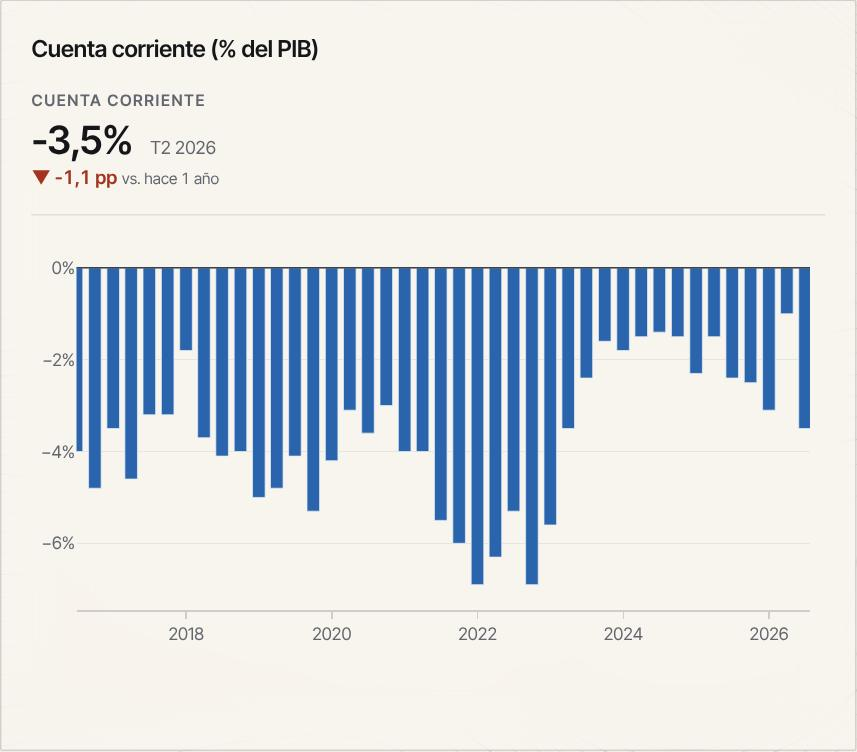
\includegraphics[width=\linewidth,height=0.42\textheight,keepaspectratio]{fig/g-cc.jpg}\end{center}
\paragraph{Qué nos cuenta}
Muestra el saldo de la cuenta corriente de la balanza de pagos como porcentaje del PIB, trimestre a trimestre. La cuenta corriente registra todo lo que el país recibe y paga al exterior por bienes, servicios, rentas (utilidades e intereses) y transferencias (como remesas). Colombia ha tenido déficit casi de forma permanente: gasta e invierte más de lo que ahorra y cubre la diferencia con recursos del resto del mundo.

\begin{leer}[Cómo se lee]
Barras azules trimestrales en porcentaje del PIB, con una línea horizontal en cero. Una barra negativa es un déficit: el país usó más recursos externos de los que generó. La vista inicial cubre los últimos diez años y se puede ampliar hacia atrás. Al pasar el cursor se ve el trimestre y el cambio frente al mismo trimestre del año anterior, en puntos porcentuales (pp). Es el dato de un solo trimestre, por lo que es más volátil que la suma de cuatro trimestres del gráfico por componentes.
\end{leer}

\paragraph{Por qué importa}
La cuenta corriente es la medida central de la posición externa de una economía. Un déficit grande y persistente significa dependencia del financiamiento externo, lo que expone al país a cambios en el apetito global por riesgo, a salidas de capital y a presiones sobre la tasa de cambio. Las calificadoras y los inversionistas en deuda colombiana lo siguen de cerca; un déficit que se cierra reduce esas vulnerabilidades.

\paragraph{Cómo interpretarlo}
\begin{itemize}
\item Barras menos negativas indican que el déficit se reduce; suele ocurrir cuando la demanda interna se enfría o cuando suben los precios de exportación.
\item Un déficit financiado con inversión extranjera directa es más estable que uno financiado con flujos de cartera o deuda de corto plazo: vea el gráfico de entradas netas de capital.
\item El dato trimestral tiene estacionalidad (por ejemplo, el giro de utilidades y dividendos se concentra en ciertos trimestres); compare siempre con el mismo trimestre del año anterior.
\item El Banco de la República revisa las cifras de balanza de pagos, en especial las de los trimestres recientes.
\end{itemize}
\begin{formulas}[Fórmulas]
\formula{Cuenta corriente (\% del PIB)}{CC\%\textsubscript{q} = CC\textsubscript{q} $\div$ PIB\textsubscript{q} $\times$ 100}{CC = bienes + servicios + ingreso primario + ingreso secundario del trimestre q; PIB del mismo trimestre (dato del Banco de la República)}
\formula{Cambio anual (al pasar el cursor)}{$\Delta$CC\%\textsubscript{q} = CC\%\textsubscript{q} − CC\%\textsubscript{q−4}}{en puntos porcentuales}
\end{formulas}
\begin{metodo}[Metodología]
Saldo de la cuenta corriente como porcentaje del PIB, trimestral. Negativo = déficit que se financia con recursos del exterior.
\par\smallskip{\small\textbf{Fuente:} Banco de la República, balanza de pagos}
\end{metodo}

\subsection{Deuda bruta del Gobierno (\% del PIB)}
\label{g:g-deuda}
\begin{center}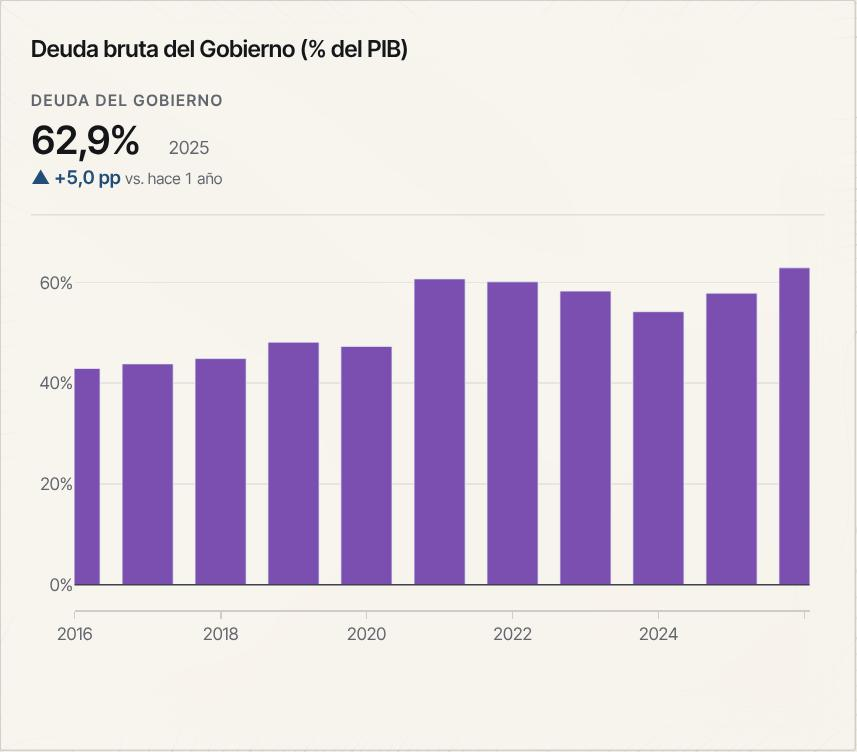
\includegraphics[width=\linewidth,height=0.42\textheight,keepaspectratio]{fig/g-deuda.jpg}\end{center}
\paragraph{Qué nos cuenta}
Muestra la deuda bruta del Gobierno Nacional Central (GNC) como porcentaje del PIB al cierre de cada año. El GNC es el Gobierno central (ministerios y entidades que dependen del presupuesto nacional), sin gobiernos regionales ni empresas públicas. La serie permite ver los grandes episodios fiscales: la crisis de finales de los noventa, la reducción de la deuda durante la bonanza de materias primas y el salto de 2020 por la pandemia.

\begin{leer}[Cómo se lee]
Barras moradas anuales, en porcentaje del PIB, con una línea horizontal en cero. Cada barra es el saldo de la deuda bruta al 31 de diciembre de ese año, incluyendo deuda interna (principalmente TES, los bonos del Tesoro en pesos) y externa. Se muestra la historia completa desde mediados de los años noventa. Al pasar el cursor se ve el cambio frente al año anterior, en puntos porcentuales (pp).
\end{leer}

\paragraph{Por qué importa}
La deuda pública es el principal indicador de sostenibilidad fiscal. Un nivel alto o creciente aumenta el pago de intereses, reduce el margen del Gobierno para responder a crisis, puede elevar las tasas de interés de toda la economía y presiona la calificación crediticia del país. Para los inversionistas en TES y en bonos externos es la referencia básica del riesgo soberano.

\paragraph{Cómo interpretarlo}
\begin{itemize}
\item La razón sube si la deuda crece más rápido que el PIB nominal: por déficit fiscales, por devaluación (que encarece en pesos la deuda en dólares) o por un crecimiento económico débil.
\item Es deuda bruta: no descuenta los activos financieros ni los depósitos del Gobierno.
\item La regla fiscal colombiana (Ley 2155 de 2021) toma como referencia la deuda neta del GNC, una medida distinta de la bruta que aquí se muestra.
\item El mismo dato, con los años por encima de 60\% del PIB resaltados, aparece en la sección de cuentas del Gobierno.
\end{itemize}
\begin{formulas}[Fórmulas]
\formula{Deuda bruta como \% del PIB}{D\%\textsubscript{a} = D\textsubscript{a} $\div$ PIB\textsubscript{a} $\times$ 100}{D = saldo de la deuda bruta del GNC al cierre del año a (interna + externa, en pesos); PIB = PIB nominal del año}
\formula{Cambio anual (al pasar el cursor)}{$\Delta$D\%\textsubscript{a} = D\%\textsubscript{a} − D\%\textsubscript{a−1}}{en puntos porcentuales}
\end{formulas}
\begin{metodo}[Metodología]
Deuda bruta del Gobierno Nacional Central como porcentaje del PIB, cierre de cada año.
\par\smallskip{\small\textbf{Fuente:} Ministerio de Hacienda, vía Banco de la República}
\end{metodo}

\section{¿De dónde viene el déficit externo?}

\subsection{Cuenta corriente por componentes (4 trimestres)}
\label{g:g-ext-cc}
\begin{center}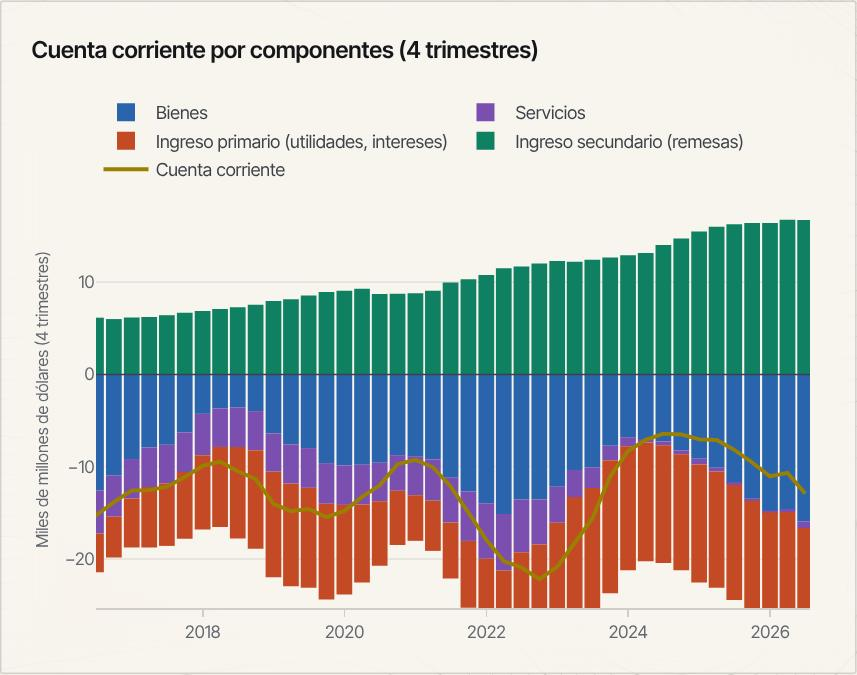
\includegraphics[width=\linewidth,height=0.42\textheight,keepaspectratio]{fig/g-ext-cc.jpg}\end{center}
\paragraph{Qué nos cuenta}
Descompone la cuenta corriente de la balanza de pagos en sus cuatro partes para mostrar de dónde viene el déficit externo de Colombia. Suele revelar que el mayor drenaje no está solo en el comercio de bienes, sino en el ingreso primario: las utilidades que las empresas extranjeras ganan en Colombia y los intereses de la deuda externa. Las remesas de los colombianos en el exterior, en cambio, compensan parte del déficit.

\begin{leer}[Cómo se lee]
Eje en miles de millones de dólares; cada punto suma los últimos cuatro trimestres, desde 2005. Barras apiladas: bienes (azul), servicios (morado), ingreso primario, es decir utilidades e intereses (naranja), e ingreso secundario, principalmente remesas (verde). Las barras por encima de cero aportan dólares y las de abajo los restan. La línea amarilla es la cuenta corriente total, igual a la suma de las cuatro barras. La línea horizontal marca el cero.
\end{leer}

\paragraph{Por qué importa}
Saber qué componente explica el déficit permite juzgar su naturaleza: un déficit de ingreso primario refleja el pago a la inversión extranjera acumulada, que tiende a moverse con la rentabilidad de las empresas (en especial petroleras y mineras); uno de bienes refleja la brecha entre gasto interno y producción. Para un inversionista ayuda a entender la demanda estructural de dólares y la sensibilidad del saldo externo al petróleo.

\paragraph{Cómo interpretarlo}
\begin{itemize}
\item Si la barra naranja (ingreso primario) se agranda cuando suben los precios de las materias primas, es porque las empresas extranjeras del sector ganan y giran más utilidades.
\item Un aumento de la barra verde (remesas) suaviza el déficit sin necesidad de financiación; vea el gráfico de remesas.
\item La línea amarilla por debajo de cero es el déficit que debe financiarse con la cuenta financiera: compárela con el gráfico de entradas netas de capital.
\item La balanza de pagos valora los bienes FOB en ambos lados, por lo que el saldo de bienes difiere del de la página de comercio (FOB − CIF).
\end{itemize}
\begin{formulas}[Fórmulas]
\formula{Suma de 4 trimestres}{Z4\textsubscript{q} = $\Sigma$\textsubscript{j=0..3} Z\textsubscript{q−j}}{Z = cada componente (millones de dólares por trimestre); se grafica en miles de millones}
\formula{Identidad de la cuenta corriente}{CC4 = B4 + S4 + IP4 + IS4}{B = bienes; S = servicios; IP = ingreso primario; IS = ingreso secundario}
\end{formulas}
\begin{metodo}[Metodología]
Suma móvil de 4 trimestres de bienes, servicios, ingreso primario e ingreso secundario; su suma es la cuenta corriente.
\par\smallskip{\small\textbf{Fuente:} Banco de la República, balanza de pagos (MBP6)}
\end{metodo}

\subsection{Exportaciones e importaciones de bienes (4 trimestres)}
\label{g:g-ext-xm}
\begin{center}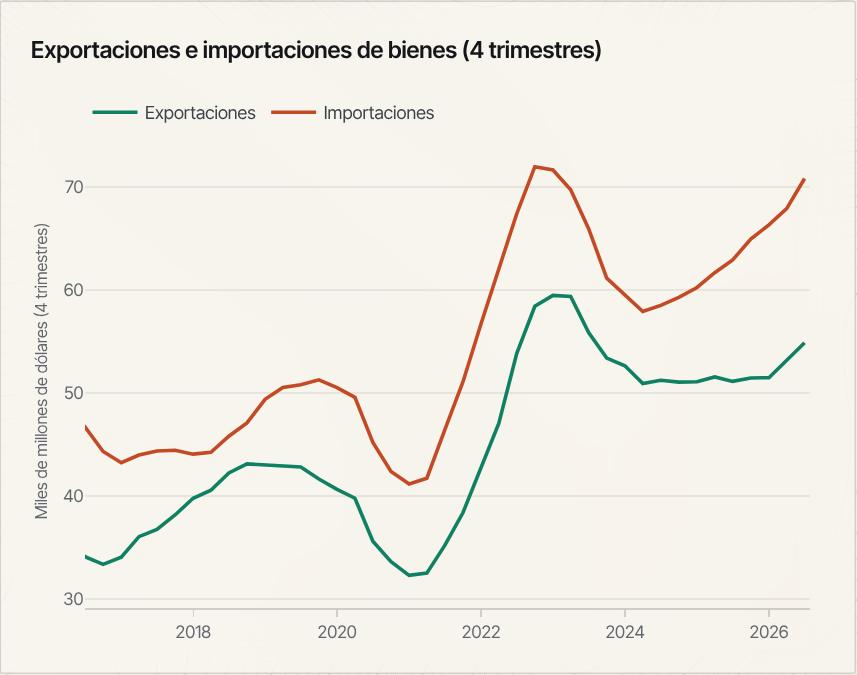
\includegraphics[width=\linewidth,height=0.42\textheight,keepaspectratio]{fig/g-ext-xm.jpg}\end{center}
\paragraph{Qué nos cuenta}
Muestra las exportaciones y las importaciones de bienes de Colombia según la balanza de pagos del Banco de la República, sumando cuatro trimestres. Es la misma historia del comercio que cuenta la página de comercio, pero con la metodología de la balanza de pagos, que valora ambos flujos en FOB y es la que se usa para la cuenta corriente. La distancia entre las dos líneas es el saldo de bienes.

\begin{leer}[Cómo se lee]
Eje en miles de millones de dólares, desde 2005. Línea verde: exportaciones de bienes (crédito de la balanza de pagos); línea naranja: importaciones de bienes (débito). Cada punto es la suma de los cuatro trimestres que terminan en ese trimestre. Cuando la naranja está por encima de la verde, el país tiene déficit en bienes; la distancia vertical entre ambas es el tamaño de ese déficit, que corresponde a la barra azul del gráfico de componentes.
\end{leer}

\paragraph{Por qué importa}
El saldo de bienes es uno de los motores principales de la cuenta corriente y, por tanto, de la necesidad de financiamiento externo. Las exportaciones dependen sobre todo de los precios del petróleo y del carbón; las importaciones, del ciclo de la demanda interna y de la inversión. Para un inversionista, esta comparación explica buena parte de los movimientos del déficit externo y de la tasa de cambio.

\paragraph{Cómo interpretarlo}
\begin{itemize}
\item Si las líneas se separan con la naranja arriba, el déficit en bienes se amplía; si se juntan, se reduce.
\item Estas cifras difieren de las del DANE porque la balanza de pagos valora las importaciones FOB (sin fletes ni seguros) y ajusta por cobertura y cambio de propiedad de las mercancías.
\item Las caídas simultáneas de ambas líneas, como en 2020, reflejan contracciones de la economía y del comercio mundial.
\item Los datos trimestrales recientes son provisionales y se revisan.
\end{itemize}
\begin{formulas}[Fórmulas]
\formula{Suma de 4 trimestres}{X4\textsubscript{q} = $\Sigma$\textsubscript{j=0..3} X\textsubscript{q−j}; M4\textsubscript{q} = $\Sigma$\textsubscript{j=0..3} M\textsubscript{q−j}}{X = exportaciones de bienes; M = importaciones de bienes (balanza de pagos, FOB)}
\formula{Saldo de bienes}{B4\textsubscript{q} = X4\textsubscript{q} − M4\textsubscript{q}}{distancia vertical entre las líneas}
\end{formulas}
\begin{metodo}[Metodología]
Exportaciones (crédito) e importaciones (débito) de bienes, suma de 4 trimestres.
\par\smallskip{\small\textbf{Fuente:} Banco de la República, balanza de pagos (MBP6)}
\end{metodo}

\section{¿Cómo se financia?}

\subsection{Entradas netas de capital por tipo (4 trimestres)}
\label{g:g-ext-financiacion}
\begin{center}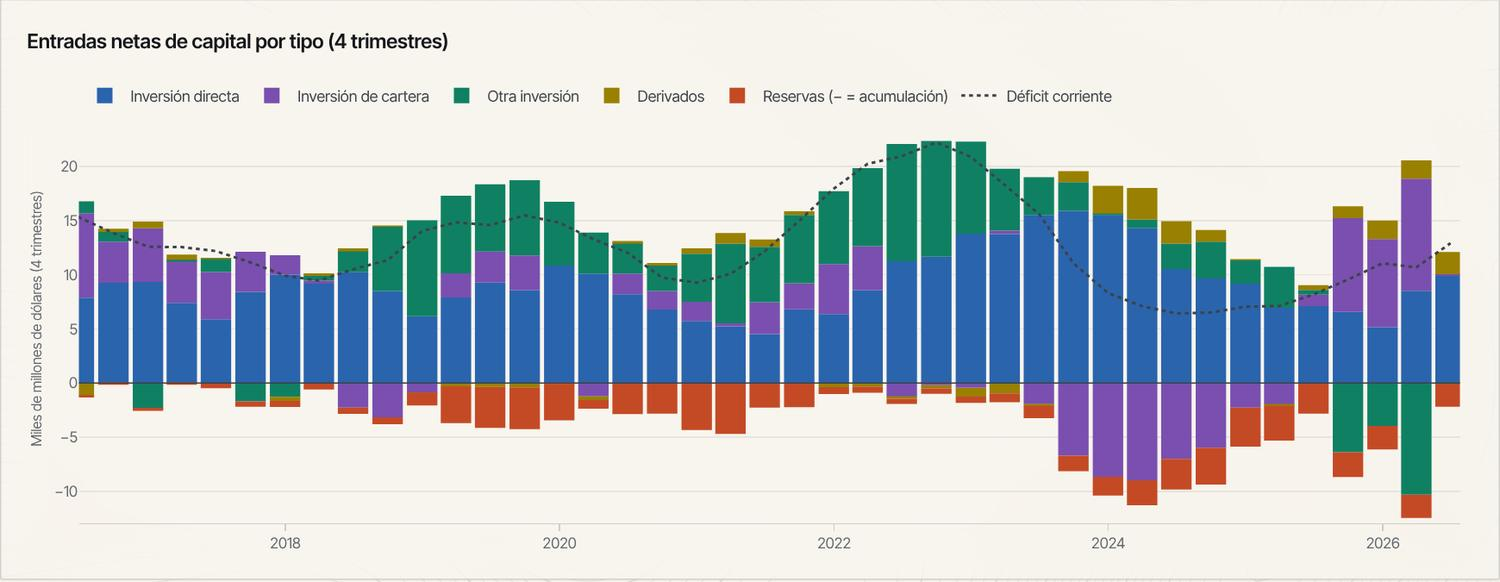
\includegraphics[width=\linewidth,height=0.42\textheight,keepaspectratio]{fig/g-ext-financiacion.jpg}\end{center}
\paragraph{Qué nos cuenta}
Muestra cómo se financia el déficit externo de Colombia: qué tipo de capital entra al país para cubrir lo que la cuenta corriente no alcanza a pagar. La historia habitual es que la inversión extranjera directa, la más estable, es la principal fuente, complementada por inversión de cartera (compras de TES y acciones por extranjeros) y préstamos, mientras el Banco de la República acumula o usa reservas internacionales.

\begin{leer}[Cómo se lee]
Barras apiladas en miles de millones de dólares, suma de cuatro trimestres, desde 2005. Cada barra es un tipo de flujo de la cuenta financiera con el signo invertido, de modo que positivo = entrada neta de financiación: inversión directa (azul), inversión de cartera (morado), otra inversión, sobre todo préstamos y depósitos (verde), derivados (amarillo) y reservas (naranja), donde un valor negativo indica acumulación de reservas. La línea gris punteada es el déficit corriente que hay que financiar.
\end{leer}

\paragraph{Por qué importa}
La calidad del financiamiento importa tanto como su monto: la inversión directa es de largo plazo y difícil de retirar, mientras que la de cartera y los préstamos de corto plazo pueden revertirse con rapidez ante cambios en el apetito por riesgo. Para un inversionista, una dependencia creciente de flujos volátiles aumenta la vulnerabilidad del peso y de los activos colombianos a choques globales.

\paragraph{Cómo interpretarlo}
\begin{itemize}
\item Si la suma de barras positivas supera la línea punteada, entra más capital del necesario y la diferencia suele terminar en acumulación de reservas (barra naranja negativa).
\item Una barra azul grande y estable es una señal de financiamiento de mejor calidad que una dependencia de cartera u otra inversión.
\item Las barras no cuadran exactamente con la línea: faltan la cuenta de capital (pequeña) y los errores y omisiones de la balanza de pagos.
\item Una inversión de cartera negativa indica que los extranjeros redujeron sus tenencias netas de bonos y acciones colombianos o que los residentes invirtieron más afuera.
\end{itemize}
\begin{formulas}[Fórmulas]
\formula{Entrada neta por tipo}{F\textsubscript{i,q} = −CF\textsubscript{i,q}}{CF\textsubscript{i} = cuenta financiera del tipo i con signo MBP6 (activos netos − pasivos netos); con signo invertido, positivo = entrada neta}
\formula{Suma de 4 trimestres}{F4\textsubscript{i,q} = $\Sigma$\textsubscript{j=0..3} F\textsubscript{i,q−j}}{i $\in$ \{directa, cartera, otra, derivados, reservas\}}
\formula{Déficit a financiar (línea punteada)}{DEF4\textsubscript{q} = −CC4\textsubscript{q}}{CC4 = cuenta corriente de 4 trimestres}
\end{formulas}
\begin{metodo}[Metodología]
Cuenta financiera por tipo de flujo con signo invertido (positivo = entrada neta), suma de 4 trimestres. Reservas: positivo = disminución.
\par\smallskip{\small\textbf{Fuente:} Banco de la República, balanza de pagos (MBP6)}
\end{metodo}

\section{Los dólares que llegan: inversión extranjera y remesas}

\subsection{Inversión extranjera directa por sector (4 trimestres)}
\label{g:g-ext-ied-sectores}
\begin{center}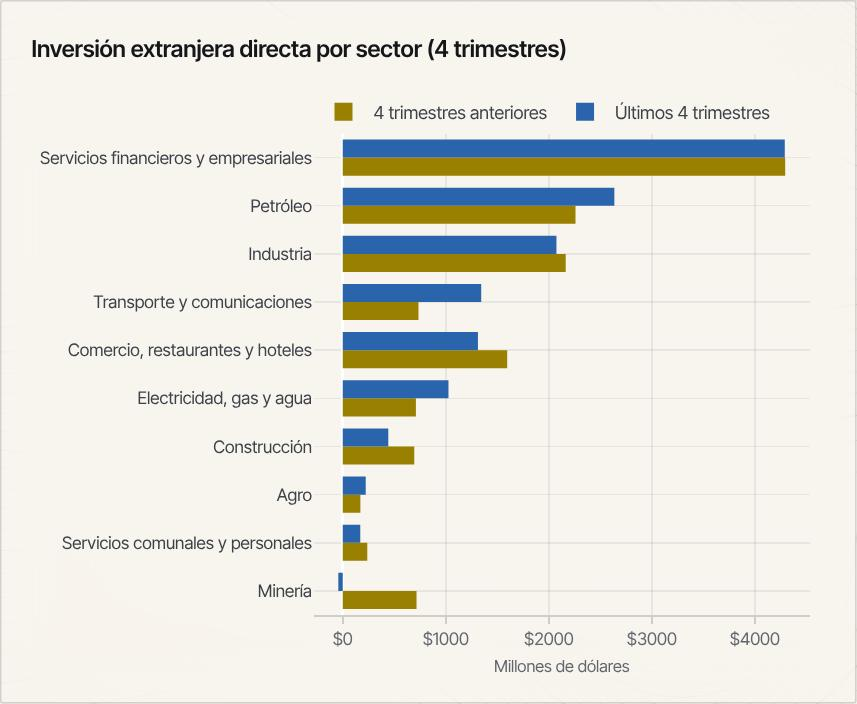
\includegraphics[width=\linewidth,height=0.42\textheight,keepaspectratio]{fig/g-ext-ied-sectores.jpg}\end{center}
\paragraph{Qué nos cuenta}
Muestra en qué sectores de la economía colombiana invierten las empresas extranjeras: la inversión extranjera directa (IED, capital que entra para crear, comprar o ampliar empresas con control o influencia duradera) de los últimos cuatro trimestres frente a los cuatro anteriores. Suele resaltar el peso del petróleo, la minería y los servicios financieros y empresariales, y permite ver qué sectores ganan o pierden atractivo.

\begin{leer}[Cómo se lee]
Barras horizontales agrupadas, una pareja por sector, en millones de dólares. Barra azul: IED de los últimos cuatro trimestres; barra amarilla: IED de los cuatro trimestres anteriores. Los sectores se ordenan según el valor de los últimos cuatro trimestres, con el mayor arriba. Son flujos netos: una barra negativa indica que las desinversiones o los pagos de préstamos entre empresas relacionadas superaron a las nuevas entradas en ese sector.
\end{leer}

\paragraph{Por qué importa}
La IED es la fuente más estable de financiamiento externo y además trae tecnología, empleo y capacidad productiva. Su composición sectorial indica si el capital extranjero se concentra en actividades extractivas, sensibles a los precios de las materias primas, o se diversifica hacia servicios, industria y energía. Para un inversionista revela en qué sectores ven oportunidades las empresas multinacionales.

\paragraph{Cómo interpretarlo}
\begin{itemize}
\item Si la barra azul supera a la amarilla, la IED en ese sector aumentó frente al año anterior; si es menor, se redujo.
\item La IED en petróleo y minería suele moverse con los precios internacionales y con la reinversión de utilidades de las empresas del sector.
\item Incluye la reinversión de utilidades: parte de la IED no es dinero nuevo que entra, sino ganancias que las filiales no giran al exterior.
\item El total de la IED y su papel en la financiación del déficit se ven en el gráfico de entradas netas de capital.
\end{itemize}
\begin{formulas}[Fórmulas]
\formula{IED de los últimos 4 trimestres}{IED4\textsubscript{s,q} = $\Sigma$\textsubscript{j=0..3} IED\textsubscript{s,q−j}}{s = sector; q = último trimestre publicado; millones de dólares}
\formula{IED de los 4 trimestres anteriores}{IED4\textsubscript{s,q−4} = $\Sigma$\textsubscript{j=4..7} IED\textsubscript{s,q−j}}{mismo cálculo, desplazado un año}
\end{formulas}
\begin{metodo}[Metodología]
Suma de los últimos 4 trimestres y de los 4 anteriores.
\par\smallskip{\small\textbf{Fuente:} Banco de la República, flujos de inversión extranjera directa por actividad}
\end{metodo}

\subsection{Remesas de los trabajadores}
\label{g:g-ext-remesas}
\begin{center}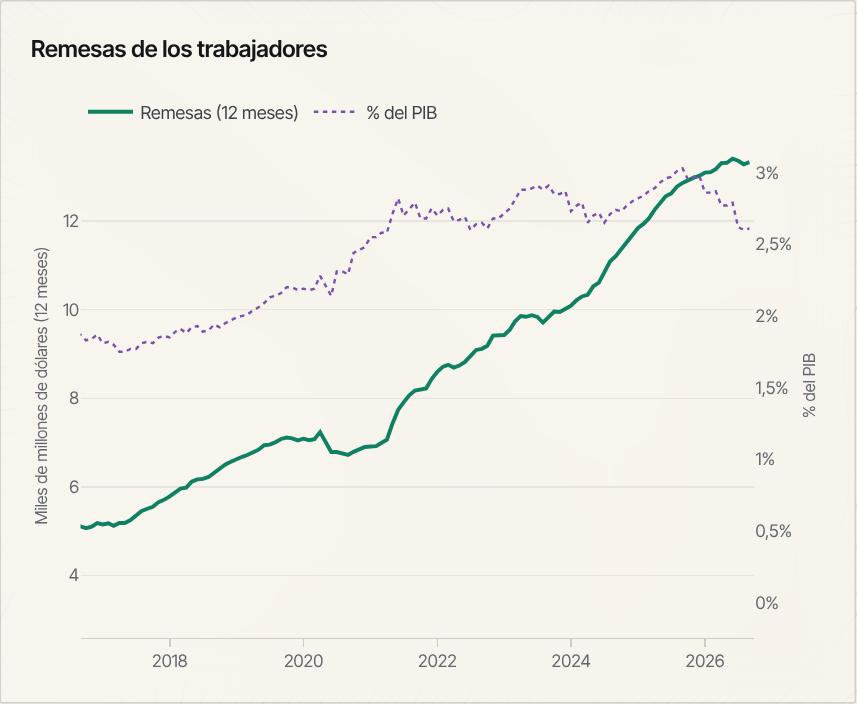
\includegraphics[width=\linewidth,height=0.42\textheight,keepaspectratio]{fig/g-ext-remesas.jpg}\end{center}
\paragraph{Qué nos cuenta}
Muestra cuántos dólares envían a Colombia los colombianos que trabajan en el exterior (remesas de trabajadores) y qué tan importantes son frente al tamaño de la economía. Las remesas se han convertido en una de las principales fuentes de divisas del país, comparable con algunas de las mayores exportaciones, y sostienen el ingreso de muchos hogares, en especial en ciertas regiones.

\begin{leer}[Cómo se lee]
Línea verde (eje izquierdo): suma de los ingresos de remesas de los últimos 12 meses, en miles de millones de dólares. Línea morada punteada (eje derecho): esa misma suma como porcentaje del PIB en dólares, calculado con el PIB nominal de los últimos cuatro trimestres disponibles convertido con la TRM (tasa de cambio oficial) promedio de cada trimestre; mientras no se publica un trimestre nuevo de PIB, se usa el último disponible. La serie empieza en 2005.
\end{leer}

\paragraph{Por qué importa}
Las remesas son un flujo de dólares estable que no genera deuda ni obligaciones futuras, por lo que ayudan a cerrar el déficit de cuenta corriente y a sostener el consumo de los hogares receptores. Dependen sobre todo del mercado laboral de Estados Unidos y España, donde vive la mayoría de los emigrantes. Para un inversionista son un soporte del peso y del consumo interno.

\paragraph{Cómo interpretarlo}
\begin{itemize}
\item Si la línea morada sube, las remesas pesan más en la economía; puede deberse a más envíos o a un PIB en dólares menor (por ejemplo, tras una devaluación).
\item Un crecimiento sostenido suele reflejar más emigración o mejores condiciones laborales en los países de destino.
\item Las remesas forman la mayor parte del ingreso secundario (barra verde) del gráfico de cuenta corriente por componentes.
\item Los datos mensuales recientes son provisionales y el Banco de la República los revisa.
\end{itemize}
\begin{formulas}[Fórmulas]
\formula{Remesas de 12 meses}{R12\textsubscript{t} = $\Sigma$\textsubscript{j=0..11} R\textsubscript{t−j}}{R = ingresos mensuales de remesas de trabajadores, en dólares}
\formula{Remesas como \% del PIB}{R\%\textsubscript{t} = R12\textsubscript{t} $\div$ Y\$4 $\times$ 100}{Y\$4 = PIB nominal de los últimos 4 trimestres disponibles, en dólares ($\Sigma$ PIB\textsubscript{q} $\div$ TRM\textsubscript{q})}
\end{formulas}
\begin{metodo}[Metodología]
Ingresos de remesas de trabajadores, suma de 12 meses; \% del PIB en dólares de los últimos 4 trimestres disponibles.
\par\smallskip{\small\textbf{Fuente:} Banco de la República (remesas); DANE (PIB nominal)}
\end{metodo}

\section{¿Cuánto le debe Colombia al exterior?}

\subsection{Deuda externa pública y privada}
\label{g:g-ext-deuda}
\begin{center}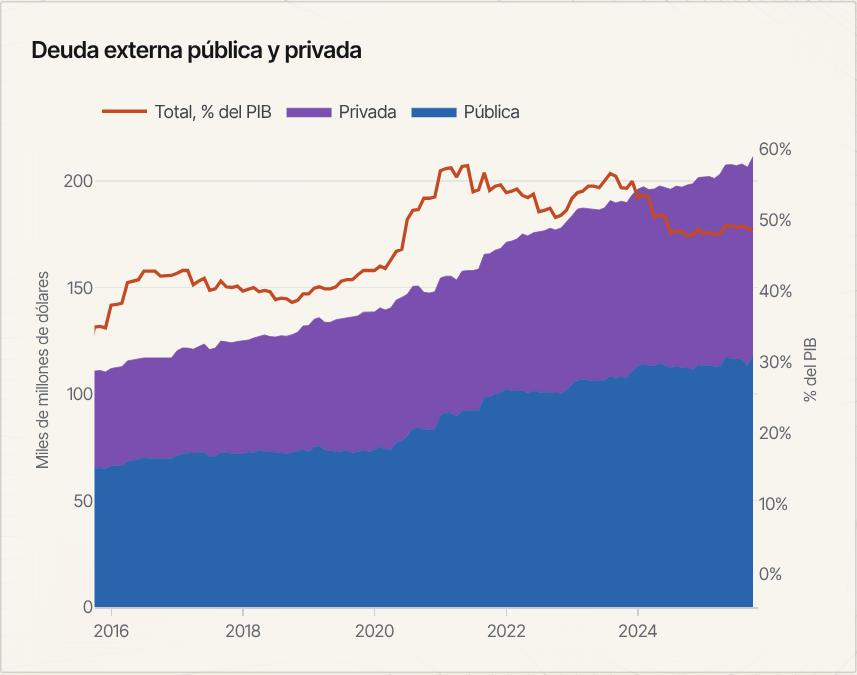
\includegraphics[width=\linewidth,height=0.42\textheight,keepaspectratio]{fig/g-ext-deuda.jpg}\end{center}
\paragraph{Qué nos cuenta}
Muestra cuánto debe Colombia al resto del mundo (deuda externa) y quién la debe: el sector público (Gobierno, entidades territoriales y empresas públicas) o el sector privado (empresas y bancos). También muestra el total en relación con el tamaño de la economía. Permite ver el aumento de la deuda externa en la última década y los cambios en su composición entre público y privado.

\begin{leer}[Cómo se lee]
Áreas apiladas (eje izquierdo) en miles de millones de dólares: azul, deuda externa pública; morado, deuda externa privada; la altura total es la deuda externa del país. Línea naranja (eje derecho, desde cero): deuda externa total como porcentaje del PIB, tal como la publica el Banco de la República. Son saldos mensuales desde 2005. Incluye préstamos y bonos emitidos en el exterior, de corto y largo plazo.
\end{leer}

\paragraph{Por qué importa}
La deuda externa debe pagarse en divisas, por lo que expone a los deudores a la tasa de cambio: una devaluación encarece su servicio en pesos. Un nivel alto como porcentaje del PIB aumenta la vulnerabilidad del país ante cierres de los mercados internacionales. Para un inversionista, la evolución de la deuda pública y privada indica el riesgo de refinanciación y la exposición cambiaria de la economía.

\paragraph{Cómo interpretarlo}
\begin{itemize}
\item La línea naranja puede subir sin que aumente la deuda en dólares: basta con que el PIB medido en dólares caiga por una devaluación del peso.
\item Si el área morada crece más rápido, el endeudamiento externo lo están impulsando las empresas y los bancos; si crece la azul, el sector público.
\item Es deuda bruta: no descuenta los activos externos del país (como las reservas internacionales); el balance completo está en la posición de inversión internacional.
\item Los saldos recientes son provisionales y pueden revisarse.
\end{itemize}
\begin{formulas}[Fórmulas]
\formula{Deuda externa total}{D\textsubscript{t} = D\textsuperscript{pública}\textsubscript{t} + D\textsuperscript{privada}\textsubscript{t}}{saldos al cierre del mes t, en dólares}
\formula{Deuda externa como \% del PIB}{D\%\textsubscript{t} = D\textsubscript{t} $\div$ PIB\$\textsubscript{t} $\times$ 100}{PIB\$ = PIB en dólares; razón calculada y publicada por el Banco de la República}
\end{formulas}
\begin{metodo}[Metodología]
Saldos mensuales de deuda externa pública y privada; total como \% del PIB según el Banco de la República.
\par\smallskip{\small\textbf{Fuente:} Banco de la República, deuda externa}
\end{metodo}

\subsection{Posición de inversión internacional}
\label{g:g-ext-pii}
\begin{center}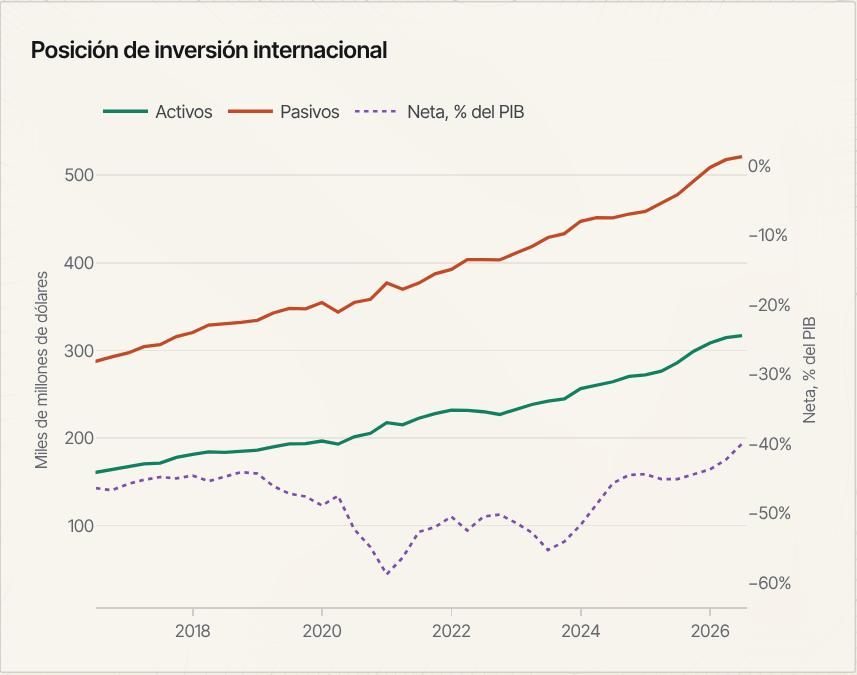
\includegraphics[width=\linewidth,height=0.42\textheight,keepaspectratio]{fig/g-ext-pii.jpg}\end{center}
\paragraph{Qué nos cuenta}
Muestra el balance financiero de Colombia con el resto del mundo: la posición de inversión internacional (PII), que compara lo que los residentes colombianos poseen en el exterior (activos) con lo que los extranjeros poseen en Colombia o les presta (pasivos). Colombia es deudora neta: sus pasivos superan a sus activos, fruto de décadas de déficit en cuenta corriente financiados con inversión extranjera y deuda.

\begin{leer}[Cómo se lee]
Eje izquierdo en miles de millones de dólares: línea verde, activos externos (incluye reservas internacionales, inversiones de residentes y depósitos en el exterior); línea naranja, pasivos externos (inversión extranjera directa y de cartera en Colombia, préstamos y deuda). Eje derecho: línea morada punteada con la posición neta (activos menos pasivos) como porcentaje del PIB en dólares de los últimos cuatro trimestres. Saldos al cierre de cada trimestre desde 2005.
\end{leer}

\paragraph{Por qué importa}
La PII neta resume la deuda acumulada del país con el exterior en todas sus formas. Un saldo muy negativo implica pagos recurrentes de utilidades e intereses (el ingreso primario de la cuenta corriente) y mayor exposición a la confianza de los inversionistas extranjeros. Para un inversionista ayuda a evaluar la vulnerabilidad externa más allá de la deuda: buena parte de los pasivos colombianos es inversión directa, que no es deuda.

\paragraph{Cómo interpretarlo}
\begin{itemize}
\item Si la distancia entre la línea naranja y la verde se amplía, el país se vuelve más deudor neto; la línea morada se hace más negativa.
\item La posición cambia no solo por los flujos, sino por cambios de valoración: variaciones de la tasa de cambio y de los precios de acciones y bonos alteran activos y pasivos sin que haya transacciones.
\item Una devaluación del peso reduce el valor en dólares de los pasivos en pesos (TES y acciones en manos de extranjeros), lo que puede mejorar la posición neta.
\item Las reservas internacionales en meses de importaciones aparecen en la tarjeta de medidas de la página.
\end{itemize}
\begin{formulas}[Fórmulas]
\formula{Posición neta}{PII\textsubscript{q} = A\textsubscript{q} − P\textsubscript{q}}{A = activos financieros externos; P = pasivos financieros externos, al cierre del trimestre q}
\formula{Posición neta como \% del PIB}{PII\%\textsubscript{q} = PII\textsubscript{q} $\div$ Y\$4\textsubscript{q} $\times$ 100}{Y\$4 = PIB nominal de 4 trimestres en dólares ($\Sigma$ PIB $\div$ TRM promedio de cada trimestre)}
\end{formulas}
\begin{metodo}[Metodología]
Activos y pasivos financieros externos al cierre de cada trimestre; posición neta sobre el PIB en dólares de 4 trimestres.
\par\smallskip{\small\textbf{Fuente:} Banco de la República, posición de inversión internacional; DANE (PIB)}
\end{metodo}

\section{Las cuentas del Gobierno}

\subsection{Ingresos, gastos e intereses del Gobierno (\% del PIB)}
\label{g:g-fi-gobierno}
\begin{center}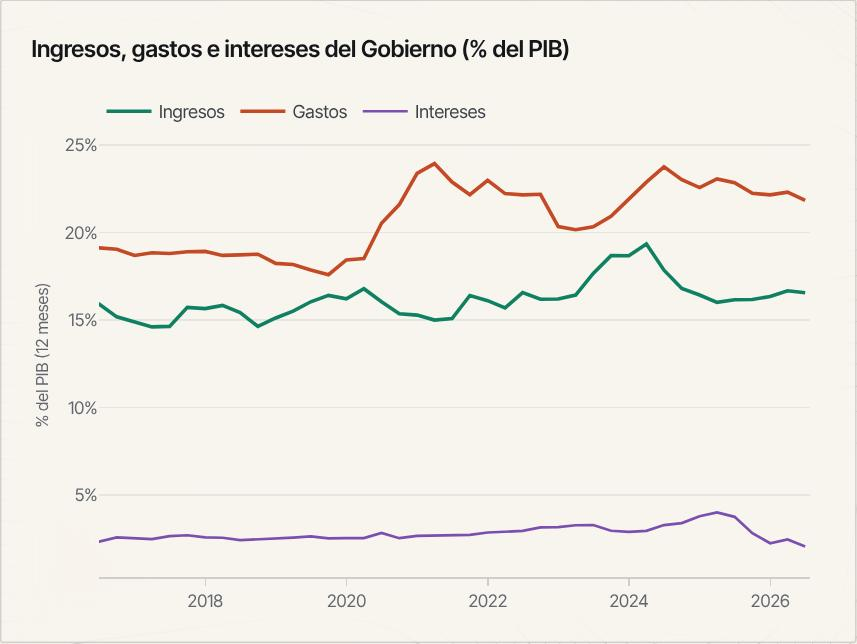
\includegraphics[width=\linewidth,height=0.42\textheight,keepaspectratio]{fig/g-fi-gobierno.jpg}\end{center}
\paragraph{Qué nos cuenta}
Muestra cuánto recauda, cuánto gasta y cuánto paga en intereses el Gobierno Nacional Central (GNC), en relación con el tamaño de la economía. La distancia entre gastos e ingresos es el déficit fiscal. Permite ver los grandes episodios fiscales: el aumento del gasto durante la pandemia de 2020, los efectos de las reformas tributarias sobre los ingresos y el peso creciente o decreciente de los intereses de la deuda.

\begin{leer}[Cómo se lee]
Tres líneas en porcentaje del PIB, desde 2005: ingresos (verde), gastos totales (naranja) e intereses de la deuda (morado), estos últimos incluidos dentro de los gastos. Las cifras son de caja (cuando el dinero efectivamente entra o sale). Para cada trimestre completo se suman los últimos cuatro trimestres de cada concepto y se dividen por el PIB nominal de esos mismos cuatro trimestres. Así se obtiene una cifra comparable a la anual en cada trimestre.
\end{leer}

\paragraph{Por qué importa}
La relación entre ingresos y gastos determina el déficit y, con él, la evolución de la deuda pública. Un gasto persistentemente superior a los ingresos obliga a endeudarse; un peso creciente de los intereses resta espacio a la inversión y al gasto social. Para un inversionista en TES y en bonos soberanos, estas cifras son la base para evaluar la sostenibilidad fiscal y el cumplimiento de la regla fiscal.

\paragraph{Cómo interpretarlo}
\begin{itemize}
\item Si la brecha entre la línea naranja y la verde se amplía, el déficit fiscal crece; si se cierra, el Gobierno necesita menos financiamiento.
\item Una línea morada en ascenso indica que la deuda o las tasas de interés pesan más en el presupuesto.
\item Las cifras de caja pueden diferir de las de causación que publica el Ministerio de Hacienda por diferencias en el momento de registro de pagos e ingresos.
\item Los ingresos tienen componentes extraordinarios (dividendos de Ecopetrol, ingresos petroleros, medidas temporales) que pueden moverlos sin cambios estructurales.
\end{itemize}
\begin{formulas}[Fórmulas]
\formula{Suma de 4 trimestres completos}{Z4\textsubscript{q} = $\Sigma$\textsubscript{j=0..3} Z\textsubscript{q−j}}{Z\textsubscript{q} = suma de los tres meses del trimestre q (solo trimestres completos); Z = ingresos, gastos o intereses}
\formula{Razón al PIB}{Z\%\textsubscript{q} = Z4\textsubscript{q} $\div$ PIB4\textsubscript{q} $\times$ 100}{PIB4 = PIB nominal de los mismos 4 trimestres, en pesos}
\end{formulas}
\begin{metodo}[Metodología]
Ingresos, gastos e intereses del Gobierno nacional central: suma de 4 trimestres completos sobre el PIB nominal de esos trimestres.
\par\smallskip{\small\textbf{Fuente:} Banco de la República (balance fiscal de caja, empalme DNP–MinHacienda); DANE (PIB nominal)}
\end{metodo}

\subsection{Balance total y primario del Gobierno (\% del PIB)}
\label{g:g-fi-balance}
\begin{center}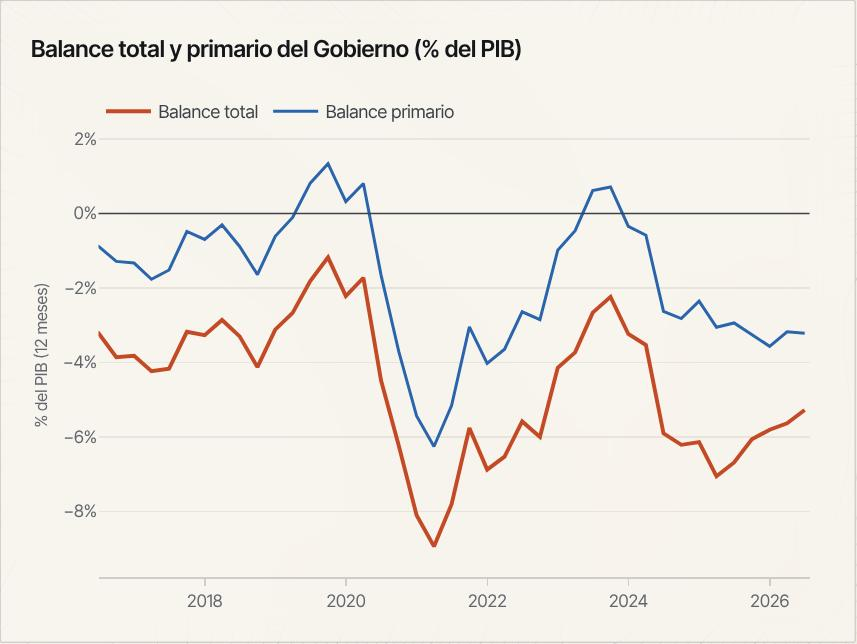
\includegraphics[width=\linewidth,height=0.42\textheight,keepaspectratio]{fig/g-fi-balance.jpg}\end{center}
\paragraph{Qué nos cuenta}
Muestra el resultado fiscal del Gobierno Nacional Central: el balance total (ingresos menos gastos) y el balance primario (el mismo resultado sin contar los intereses de la deuda). El balance primario indica si el Gobierno cubre con sus ingresos el gasto corriente y de inversión antes de pagar la deuda; el total incluye el costo de la deuda acumulada. Permite ver episodios como el gran déficit de 2020 y los esfuerzos posteriores de ajuste.

\begin{leer}[Cómo se lee]
Dos líneas en porcentaje del PIB, desde 2005, con una línea horizontal en cero. Línea naranja: balance total. Línea azul: balance primario, igual al balance total más los intereses. Valores negativos son déficit y positivos superávit. Cifras de caja, sumando los últimos cuatro trimestres completos y dividiendo por el PIB nominal de esos mismos trimestres. La distancia entre las dos líneas es el pago de intereses.
\end{leer}

\paragraph{Por qué importa}
El balance primario es la variable clave de la sostenibilidad de la deuda: si es positivo y suficiente frente a la diferencia entre la tasa de interés y el crecimiento de la economía, la deuda como porcentaje del PIB tiende a estabilizarse o bajar. La regla fiscal colombiana (Ley 2155 de 2021) fija su meta sobre el balance primario neto estructural, una medida relacionada pero ajustada por el ciclo y los ingresos petroleros. Para un inversionista en deuda soberana es la medida más directa del esfuerzo fiscal del Gobierno.

\paragraph{Cómo interpretarlo}
\begin{itemize}
\item Un balance primario positivo significa que el Gobierno genera recursos para pagar parte de los intereses; uno negativo, que se endeuda incluso para gastos distintos de la deuda.
\item Si la distancia entre las líneas crece, los intereses pesan más en el déficit total.
\item La deuda como porcentaje del PIB se estabiliza aproximadamente cuando el balance primario iguala (r − g) $\times$ deuda $\div$ (1 + g), donde r es la tasa de interés implícita y g el crecimiento nominal.
\item En cifras de caja, los intereses pueden mostrar meses con valores atípicos o negativos (por ejemplo, primas en colocaciones de bonos), lo que también afecta al balance primario.
\end{itemize}
\begin{formulas}[Fórmulas]
\formula{Balance total}{BT\textsubscript{q} = (I4\textsubscript{q} − G4\textsubscript{q}) $\div$ PIB4\textsubscript{q} $\times$ 100}{I = ingresos; G = gastos totales (incluyen intereses); sumas de 4 trimestres}
\formula{Balance primario}{BP\textsubscript{q} = BT\textsubscript{q} + INT4\textsubscript{q} $\div$ PIB4\textsubscript{q} $\times$ 100}{INT = intereses de la deuda en 4 trimestres}
\end{formulas}
\begin{metodo}[Metodología]
Balance total = déficit/superávit de caja; primario = balance total + intereses.
\par\smallskip{\small\textbf{Fuente:} Banco de la República (balance fiscal de caja, empalme DNP–MinHacienda); DANE (PIB nominal)}
\end{metodo}

\subsection{Deuda bruta del Gobierno nacional central (\% del PIB)}
\label{g:g-fi-deuda}
\begin{center}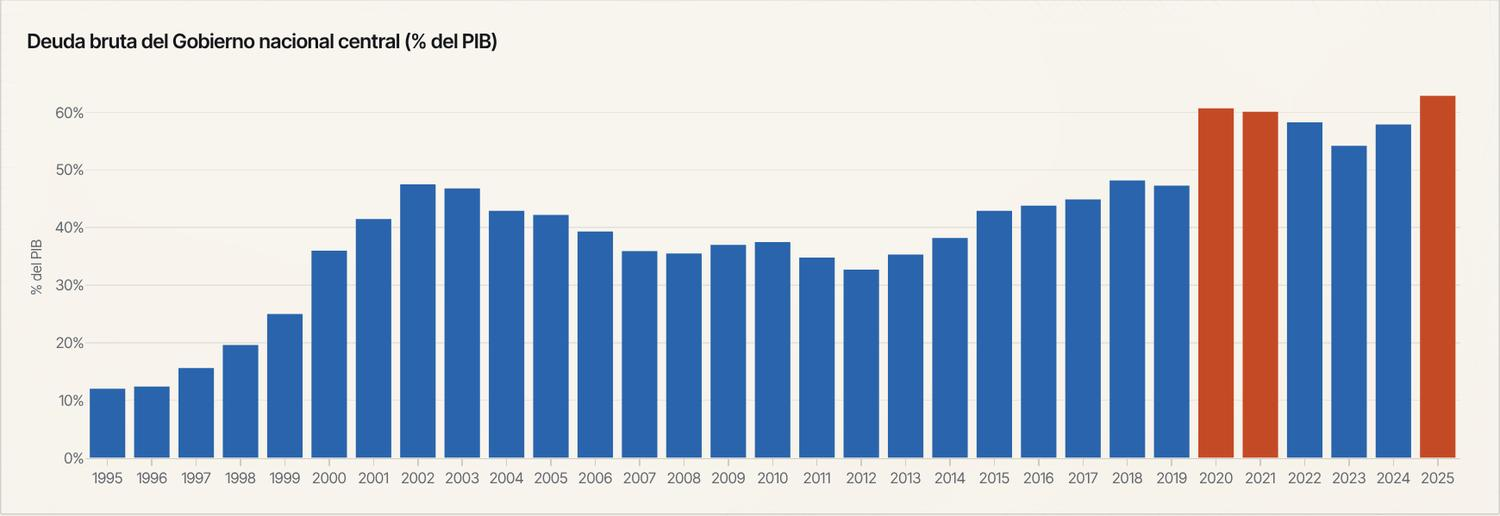
\includegraphics[width=\linewidth,height=0.42\textheight,keepaspectratio]{fig/g-fi-deuda.jpg}\end{center}
\paragraph{Qué nos cuenta}
Muestra la deuda bruta del Gobierno Nacional Central (GNC) como porcentaje del PIB al cierre de cada año, resaltando los años en que superó el 60\% del PIB. Resume la historia fiscal de tres décadas: el aumento de la deuda tras la crisis de finales de los noventa, su reducción en los años de bonanza, el nuevo ascenso tras la caída del petróleo y el salto de 2020 por la pandemia.

\begin{leer}[Cómo se lee]
Barras anuales en porcentaje del PIB, desde mediados de los años noventa. Barras azules: años con deuda igual o inferior al 60\% del PIB; barras naranjas: años por encima de ese nivel. Cada barra es el saldo al 31 de diciembre de la deuda interna (principalmente TES, los bonos del Tesoro en pesos) y externa del GNC. Al pasar el cursor se ve el valor exacto de cada año.
\end{leer}

\paragraph{Por qué importa}
El nivel de deuda condiciona el costo de financiamiento del Gobierno, la calificación crediticia del país y el margen para responder a choques. El umbral de 60\% del PIB es una referencia internacional habitual de deuda elevada para economías emergentes, usada aquí solo como guía visual. Para un inversionista en TES y bonos externos, la trayectoria de la deuda es el punto de partida del análisis de riesgo soberano.

\paragraph{Cómo interpretarlo}
\begin{itemize}
\item Barras naranjas indican niveles de deuda que tradicionalmente se asocian a mayor riesgo para economías emergentes; el umbral es una referencia, no un límite legal.
\item La deuda puede subir por déficit fiscales, por devaluación del peso (la deuda externa vale más en pesos) o por un crecimiento nominal débil.
\item La regla fiscal colombiana fija su ancla sobre la deuda neta, no sobre la bruta; las dos medidas difieren por los activos financieros del Gobierno.
\item El balance fiscal que explica los cambios de la deuda se ve en los gráficos de ingresos, gastos y balance.
\end{itemize}
\begin{formulas}[Fórmulas]
\formula{Deuda bruta como \% del PIB}{D\%\textsubscript{a} = D\textsubscript{a} $\div$ PIB\textsubscript{a} $\times$ 100}{D = saldo de la deuda bruta del GNC al cierre del año a; PIB = PIB nominal del año}
\formula{Color de la barra}{naranja si D\%\textsubscript{a} > 60; azul en otro caso}{umbral de referencia de 60\% del PIB}
\end{formulas}
\begin{metodo}[Metodología]
Saldo anual; en naranja los años por encima de 60\% del PIB.
\par\smallskip{\small\textbf{Fuente:} Banco de la República (deuda bruta del GNC, \% del PIB)}
\end{metodo}

\section{¿Cómo se financia el Gobierno y cuánto le cuesta?}

\subsection{Financiamiento del Gobierno e intereses}
\label{g:g-fi-financiamiento}
\begin{center}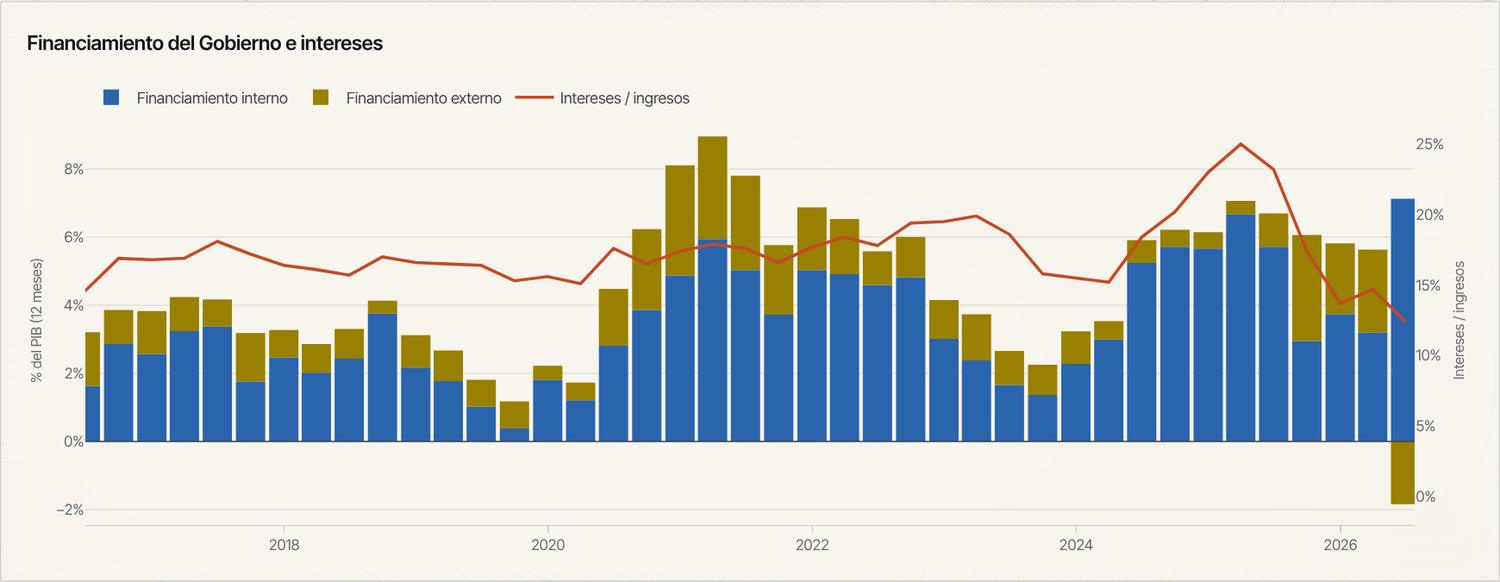
\includegraphics[width=\linewidth,height=0.42\textheight,keepaspectratio]{fig/g-fi-financiamiento.jpg}\end{center}
\paragraph{Qué nos cuenta}
Muestra cómo cubre el Gobierno Nacional Central su déficit (con recursos internos o externos) y cuánto de sus ingresos se le va en pagar intereses de la deuda. El financiamiento interno proviene sobre todo de la colocación de TES (bonos del Tesoro en pesos) en el mercado local; el externo, de bonos en el exterior y créditos de organismos multilaterales. La línea de intereses mide la carga de la deuda sobre el presupuesto.

\begin{leer}[Cómo se lee]
Barras apiladas (eje izquierdo) en porcentaje del PIB, suma de cuatro trimestres completos sobre el PIB nominal de esos trimestres, desde 2005: financiamiento interno (azul) y externo (amarillo). Un valor negativo indica que en neto se pagó más deuda de esa fuente de la que se tomó. Por construcción, la suma de las dos barras equivale al déficit de caja. Línea naranja (eje derecho, desde cero): intereses pagados por cada \$100 de ingresos del Gobierno en esos mismos cuatro trimestres.
\end{leer}

\paragraph{Por qué importa}
La mezcla entre financiamiento interno y externo determina la exposición del Gobierno a la tasa de cambio y su dependencia del mercado local de TES, donde también participan bancos, fondos de pensiones e inversionistas extranjeros. La carga de intereses sobre ingresos es un indicador directo de cuánta capacidad fiscal absorbe la deuda: cuanto mayor, menos espacio queda para otros gastos. Es una referencia básica para inversionistas en deuda pública.

\paragraph{Cómo interpretarlo}
\begin{itemize}
\item Una línea naranja en ascenso indica que una parte creciente del recaudo se destina a intereses, por mayor deuda, tasas más altas o ingresos más débiles.
\item Más financiamiento interno implica más oferta de TES en el mercado local, lo que puede presionar sus tasas; más financiamiento externo eleva la exposición a la tasa de cambio.
\item Una barra externa negativa puede reflejar amortizaciones de deuda externa o su sustitución por deuda interna.
\item Los intereses de caja tienen meses atípicos o negativos (por ejemplo, primas en colocaciones), por lo que este indicador puede quedar por debajo del costo de la deuda en causación que reporta el Ministerio de Hacienda.
\end{itemize}
\begin{formulas}[Fórmulas]
\formula{Financiamiento como \% del PIB}{F\%\textsubscript{q} = F4\textsubscript{q} $\div$ PIB4\textsubscript{q} $\times$ 100}{F4 = financiamiento interno o externo de 4 trimestres completos; PIB4 = PIB nominal de los mismos trimestres}
\formula{Identidad de financiamiento}{F\textsuperscript{int} + F\textsuperscript{ext} = −BT}{BT = balance total de caja (negativo si hay déficit)}
\formula{Intereses por cada \$100 de ingresos}{II\textsubscript{q} = INT4\textsubscript{q} $\div$ I4\textsubscript{q} $\times$ 100}{INT4 = intereses; I4 = ingresos; ambos sumas de 4 trimestres}
\end{formulas}
\begin{metodo}[Metodología]
Financiamiento interno y externo, suma de 4 trimestres sobre el PIB; intereses sobre ingresos de los mismos 4 trimestres.
\par\smallskip{\small\textbf{Fuente:} Banco de la República (balance fiscal de caja, empalme DNP–MinHacienda); DANE (PIB nominal)}
\end{metodo}

\section*{Lecturas de la página}
\begin{itemize}\small
\item \textbf{Obstfeld, M. y Rogoff, K. (1995). The Intertemporal Approach to the Current Account. En Handbook of International Economics, vol. 3, 1731–1799.} Por qué un país ahorra o se endeuda con el exterior.
\item \textbf{Calvo, G. A., Leiderman, L. y Reinhart, C. M. (1993). Capital Inflows and Real Exchange Rate Appreciation in Latin America. IMF Staff Papers, 40(1), 108–151.} El papel de los flujos de capital y los factores externos en América Latina.
\item \textbf{Lane, P. R. y Milesi-Ferretti, G. M. (2007). The External Wealth of Nations Mark II. Journal of International Economics, 73(2), 223–250.} Cómo se mide y qué revela la posición de inversión internacional.
\item \textbf{Reinhart, C. M. y Rogoff, K. S. (2009). This Time Is Different: Eight Centuries of Financial Folly. Princeton University Press.} Deuda pública y externa en perspectiva histórica.
\item \textbf{Blanchard, O. (2019). Public Debt and Low Interest Rates. American Economic Review, 109(4), 1197–1229.} Cuándo la deuda pública es sostenible: tasa de interés frente a crecimiento.
\item \textbf{FMI (2009). Manual de Balanza de Pagos y Posición de Inversión Internacional, sexta edición (MBP6).} Metodología con la que el Banco de la República elabora la balanza de pagos.
\item \textbf{Ley 1473 de 2011 y Ley 2155 de 2021: regla fiscal de Colombia y Comité Autónomo de la Regla Fiscal.} Marco legal que limita el déficit y la deuda del Gobierno nacional central.
\end{itemize}

\chapter{Comercio exterior}
\label{atlas:comercio}

{\large\sffamily\bfseries Comercio exterior: qué vende y qué compra Colombia\par}\medskip

Exportaciones e importaciones de bienes con las cifras oficiales del DANE y la DIAN: cuánto, qué, para qué y con quién.

{\small\color{cmmuted}Página del sitio: \url{https://stv-quant.github.io/ColombiaMacro-USBCali/comercio/}}

\section{¿Cuánto vende y cuánto compra Colombia?}

\subsection{Exportaciones e importaciones, suma de 12 meses}
\label{g:g-comercio-flujos}
\begin{center}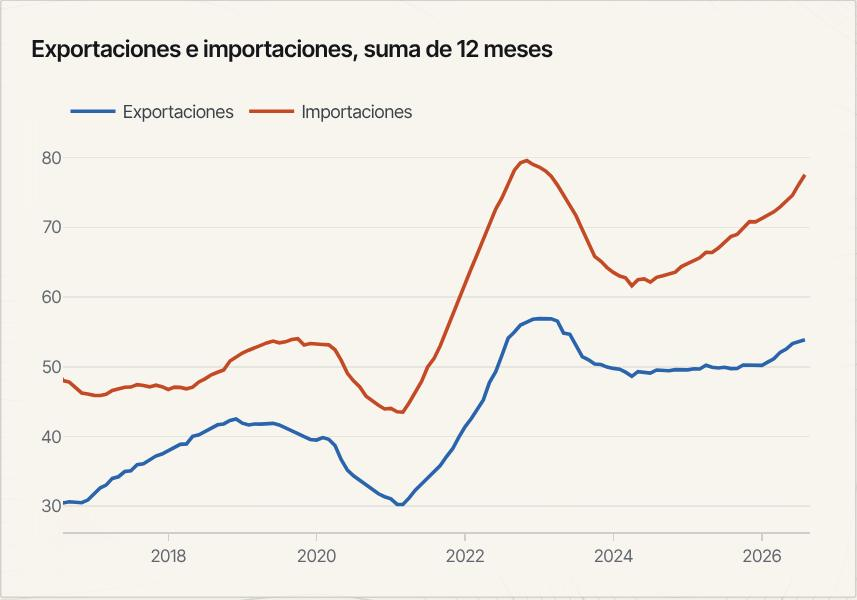
\includegraphics[width=\linewidth,height=0.42\textheight,keepaspectratio]{fig/g-comercio-flujos.jpg}\end{center}
\paragraph{Qué nos cuenta}
Muestra cuánto vende Colombia al resto del mundo (exportaciones de bienes) y cuánto le compra (importaciones), sumando siempre los últimos 12 meses. La distancia entre las dos líneas es la balanza comercial de bienes. La historia que cuenta es la del ciclo de las materias primas: las exportaciones suben y bajan con el precio del petróleo y del carbón, mientras las importaciones siguen más de cerca a la demanda interna y a la inversión. Se ven, por ejemplo, el desplome de ambas en 2020 y el rebote posterior.

\begin{leer}[Cómo se lee]
Eje vertical en miles de millones de dólares corrientes, desde cero. Línea azul: exportaciones FOB (valor de la mercancía en el puerto colombiano, sin fletes ni seguros); línea naranja: importaciones CIF (incluyen costo, seguro y flete hasta Colombia). Cada punto es la suma de los 12 meses que terminan en ese mes. Las exportaciones arrancan en los años noventa; las importaciones, cuando empieza la serie mensual del DANE disponible en el sitio. Cuando la naranja va por encima de la azul hay déficit comercial.
\end{leer}

\paragraph{Por qué importa}
El comercio de bienes es la principal fuente de dólares de la economía y el componente más grande de la cuenta corriente. Un déficit comercial amplio debe cubrirse con inversión extranjera, endeudamiento externo o remesas, y su tamaño influye en la tasa de cambio. Para un inversionista, las exportaciones indican el ingreso externo del país y de los sectores minero-energéticos; las importaciones reflejan el pulso del consumo de bienes durables y de la compra de maquinaria.

\paragraph{Cómo interpretarlo}
\begin{itemize}
\item Si la brecha entre la línea naranja y la azul se amplía, el déficit comercial crece y el país necesita más financiación externa; si se cierra, depende menos de ella.
\item Las exportaciones pueden caer solo por menores precios internacionales, sin que se venda menos cantidad: compárelo con el gráfico de valor, precio y volumen.
\item La suma de 12 meses elimina la estacionalidad sin modelos, pero reacciona con rezago: un cambio fuerte de un mes tarda en verse completo.
\item Las cifras son en dólares corrientes, sin ajuste por inflación externa; los últimos meses son provisionales y el DANE los revisa.
\item Esta balanza (FOB menos CIF) es algo más negativa que la de bienes de la balanza de pagos de la página Externo, que valora ambas en FOB.
\end{itemize}
\begin{formulas}[Fórmulas]
\formula{Suma de 12 meses}{X12\textsubscript{t} = $\Sigma$\textsubscript{j=0..11} X\textsubscript{t−j}}{X = exportaciones (o importaciones) del mes; t = mes; resultado en miles de millones de dólares}
\formula{Balanza comercial de 12 meses}{B12\textsubscript{t} = X12\textsubscript{t} − M12\textsubscript{t}}{X12 = exportaciones FOB; M12 = importaciones CIF, ambas sumas de 12 meses}
\end{formulas}
\begin{metodo}[Metodología]
Exportaciones FOB (valor en el puerto colombiano) e importaciones CIF (incluyen seguro y flete), en dólares corrientes. Cada punto es la suma móvil de 12 meses, que elimina la estacionalidad sin modelos. Las cifras del último año son provisionales.
\par\smallskip{\small\textbf{Fuente:} DANE con registros de la DIAN: exportaciones e importaciones}
\end{metodo}

\subsection{Balanza comercial por año}
\label{g:g-balanza}
\begin{center}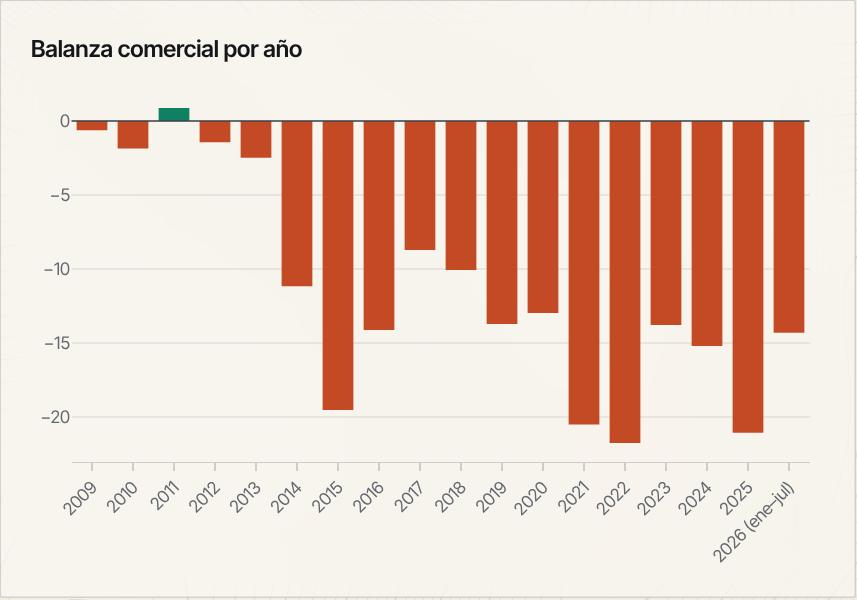
\includegraphics[width=\linewidth,height=0.42\textheight,keepaspectratio]{fig/g-balanza.jpg}\end{center}
\paragraph{Qué nos cuenta}
Resume, año por año, si Colombia vendió al exterior más bienes de los que compró (superávit) o menos (déficit). Permite ver de un vistazo los periodos en que la bonanza de precios de las materias primas dejó saldos cercanos a cero o positivos y el cambio de régimen tras la caída del precio del petróleo de mediados de la década pasada, desde la cual el saldo ha sido persistentemente negativo.

\begin{leer}[Cómo se lee]
Cada barra es un año calendario, en miles de millones de dólares: exportaciones FOB menos importaciones CIF, sumando los meses del año. Barras verdes: superávit; barras naranjas: déficit. La línea horizontal marca el cero. La serie empieza con el primer año en que hay datos mensuales de importaciones en el sitio. El último año aparece con la etiqueta «ene–mes» cuando está incompleto: suma solo de enero al último mes publicado y no es comparable con un año completo.
\end{leer}

\paragraph{Por qué importa}
El saldo comercial anual es la referencia más usada para describir la posición externa del país en bienes. Un déficit persistente implica una necesidad estructural de dólares que se cubre con capitales externos, y hace a la economía más sensible a los cambios en el apetito internacional por riesgo. Para un inversionista ayuda a dimensionar la presión sobre el peso y la dependencia del financiamiento externo.

\paragraph{Cómo interpretarlo}
\begin{itemize}
\item Una barra naranja más larga que la del año anterior indica que el déficit se amplió; puede deberse a menores exportaciones, a mayores importaciones o a ambas: revise el gráfico de flujos de 12 meses.
\item La barra parcial del año en curso debe compararse con el acumulado del mismo periodo del año anterior, no con el total anual.
\item Como las importaciones incluyen flete y seguro (CIF), este saldo es algo más negativo que el de bienes de la balanza de pagos del Banco de la República, que usa FOB en ambos lados.
\item Las cifras de los meses recientes son provisionales y pueden revisarse.
\end{itemize}
\begin{formulas}[Fórmulas]
\formula{Balanza anual}{B\textsubscript{a} = $\Sigma$\textsubscript{m$\in$a} X\textsubscript{m} − $\Sigma$\textsubscript{m$\in$a} M\textsubscript{m}}{X = exportaciones FOB; M = importaciones CIF; m = meses del año a (en el año en curso, solo los publicados)}
\end{formulas}
\begin{metodo}[Metodología]
Balanza = exportaciones FOB − importaciones CIF de cada año calendario (sumas mensuales del DANE). Como las importaciones incluyen flete y seguro, este saldo es algo más negativo que el de la balanza de pagos del Banco de la República (que usa FOB en ambos lados).
\par\smallskip{\small\textbf{Fuente:} DANE con registros de la DIAN: exportaciones e importaciones}
\end{metodo}

\section{¿Qué vende Colombia?}

\subsection{¿Qué vende? Exportaciones de los últimos 12 meses}
\label{g:g-expo-productos}
\begin{center}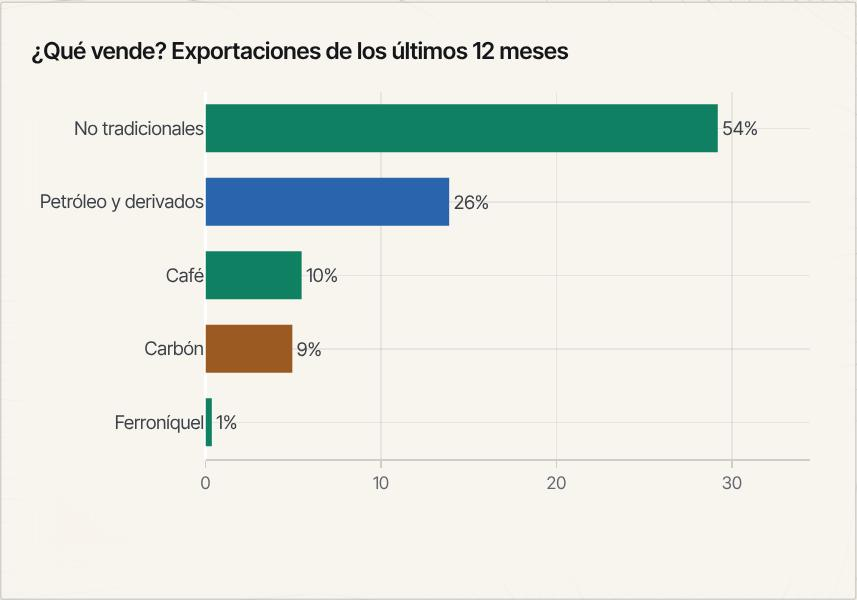
\includegraphics[width=\linewidth,height=0.42\textheight,keepaspectratio]{fig/g-expo-productos.jpg}\end{center}
\paragraph{Qué nos cuenta}
Muestra qué vende Colombia al exterior en los últimos 12 meses, según los cinco grupos con que el DANE clasifica las exportaciones: los cuatro productos tradicionales (petróleo y derivados, carbón, café y ferroníquel) y los no tradicionales, que agrupan todo lo demás (manufacturas, agroindustria, flores, banano, químicos, entre otros). Revela el grado de concentración de la canasta exportadora en unos pocos bienes básicos.

\begin{leer}[Cómo se lee]
Barras horizontales ordenadas de mayor a menor. El largo de cada barra es el valor exportado en 12 meses, en miles de millones de dólares FOB; el número al final es su participación en el total. Colores: azul para petróleo y derivados, café oscuro para carbón y verde para los demás grupos. Al pasar el cursor aparece la variación frente a los 12 meses anteriores, en dólares.
\end{leer}

\paragraph{Por qué importa}
La composición de las exportaciones determina qué tan expuestos están los ingresos externos, el recaudo y la tasa de cambio a los precios internacionales de unos pocos bienes. Una canasta dominada por petróleo y carbón transmite con fuerza los choques de precios a la economía; un peso mayor de los no tradicionales suele asociarse a ingresos externos más estables y a más empresas y regiones vinculadas al comercio.

\paragraph{Cómo interpretarlo}
\begin{itemize}
\item Una variación anual fuerte en petróleo o carbón suele reflejar sobre todo precios internacionales; en café influyen además el clima y la cosecha.
\item Si la participación de los no tradicionales sube, la canasta se diversifica; el gráfico de peso del petróleo y el carbón muestra esa evolución en el tiempo.
\item Los no tradicionales son un grupo muy heterogéneo: su total no permite saber qué producto concreto creció.
\item Las variaciones están en dólares corrientes, así que mezclan cambios de precio y de cantidad; las cifras recientes son provisionales.
\end{itemize}
\begin{formulas}[Fórmulas]
\formula{Valor de 12 meses del grupo k}{X12\textsubscript{k,t} = $\Sigma$\textsubscript{j=0..11} X\textsubscript{k,t−j}}{X\textsubscript{k} = exportaciones FOB del grupo k en el mes}
\formula{Participación}{s\textsubscript{k} = X12\textsubscript{k,t} $\div$ X12\textsubscript{t} $\times$ 100}{X12\textsubscript{t} = exportaciones totales de 12 meses}
\formula{Variación anual (al pasar el cursor)}{g\textsubscript{k} = (X12\textsubscript{k,t} $\div$ X12\textsubscript{k,t−12} − 1) $\times$ 100}{compara con los 12 meses que terminan un año antes}
\end{formulas}
\begin{metodo}[Metodología]
Suma de los últimos 12 meses por grupo del DANE: café, carbón, petróleo y derivados, ferroníquel (tradicionales) y no tradicionales. Variación: frente a los 12 meses anteriores, en dólares.
\par\smallskip{\small\textbf{Fuente:} DANE con registros de la DIAN: exportaciones (anexos estadísticos)}
\end{metodo}

\subsection{Peso del petróleo y el carbón en las exportaciones}
\label{g:g-expo-minero}
\begin{center}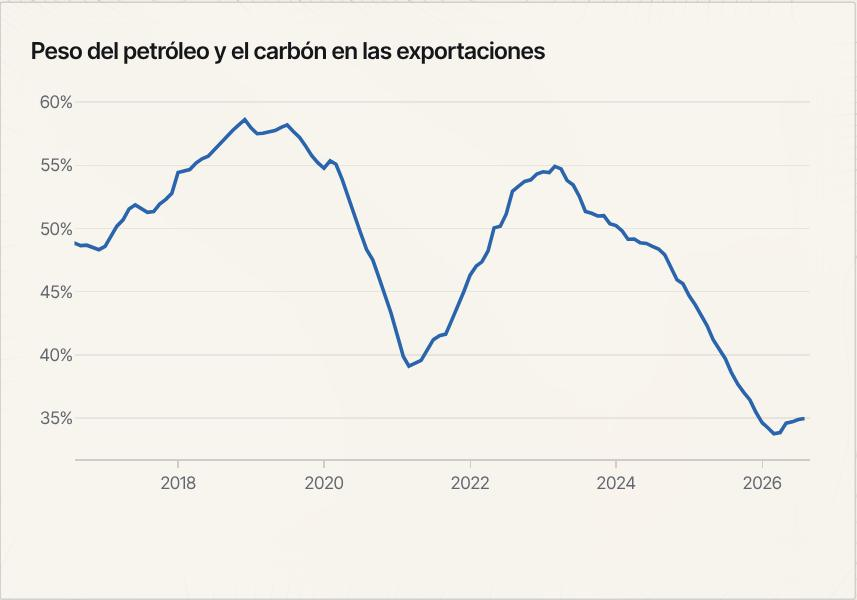
\includegraphics[width=\linewidth,height=0.42\textheight,keepaspectratio]{fig/g-expo-minero.jpg}\end{center}
\paragraph{Qué nos cuenta}
Muestra qué parte de todo lo que Colombia exporta corresponde a petróleo y sus derivados más carbón, los dos productos minero-energéticos que han dominado la canasta. Es una medida directa de la dependencia del país de estos bienes: se dispara en los auges de precios de las materias primas, como la bonanza de inicios de la década de 2010, y cae cuando esos precios se desploman o cuando crecen otras ventas.

\begin{leer}[Cómo se lee]
Una sola línea azul, en porcentaje de las exportaciones totales, con eje fijo de 0\% a 80\%. Cada punto divide la suma de 12 meses de las exportaciones de petróleo y derivados más carbón entre la suma de 12 meses de las exportaciones totales, ambas en dólares FOB. La serie empieza a mediados de los años noventa. Una línea descendente indica menor peso minero-energético.
\end{leer}

\paragraph{Por qué importa}
Cuanto mayor es esta participación, más dependen de los precios internacionales de la energía la entrada de dólares, la tasa de cambio, las regalías y los ingresos del Gobierno. Para un inversionista indica la sensibilidad de la economía colombiana al ciclo petrolero y la vulnerabilidad de las cuentas externas y fiscales ante una caída de precios.

\paragraph{Cómo interpretarlo}
\begin{itemize}
\item Una caída puede deberse a que la minería se vende más barata (efecto precio) o a que crecen más los demás productos; no siempre implica una diversificación genuina.
\item Saltos bruscos coinciden con choques de precios del petróleo; compárelo con el gráfico de valor, precio y volumen de las exportaciones.
\item No incluye otros minerales como oro o ferroníquel, que el DANE clasifica de forma distinta.
\item Como usa sumas de 12 meses, el indicador se mueve gradualmente y no capta la estacionalidad de un mes aislado.
\end{itemize}
\begin{formulas}[Fórmulas]
\formula{Peso minero-energético}{S\textsubscript{t} = (P12\textsubscript{t} + C12\textsubscript{t}) $\div$ X12\textsubscript{t} $\times$ 100}{P12 = petróleo y derivados; C12 = carbón; X12 = exportaciones totales; todas sumas de 12 meses en dólares FOB}
\end{formulas}
\begin{metodo}[Metodología]
(Petróleo y derivados + carbón) / exportaciones totales, con sumas móviles de 12 meses. Depende de precios internacionales y volúmenes.
\par\smallskip{\small\textbf{Fuente:} DANE con registros de la DIAN: exportaciones (anexos estadísticos)}
\end{metodo}

\section{¿Qué compra y para qué?}

\subsection{¿Para qué importa? Variación enero–julio 2026 frente a 2025}
\label{g:g-impo-uso}
\begin{center}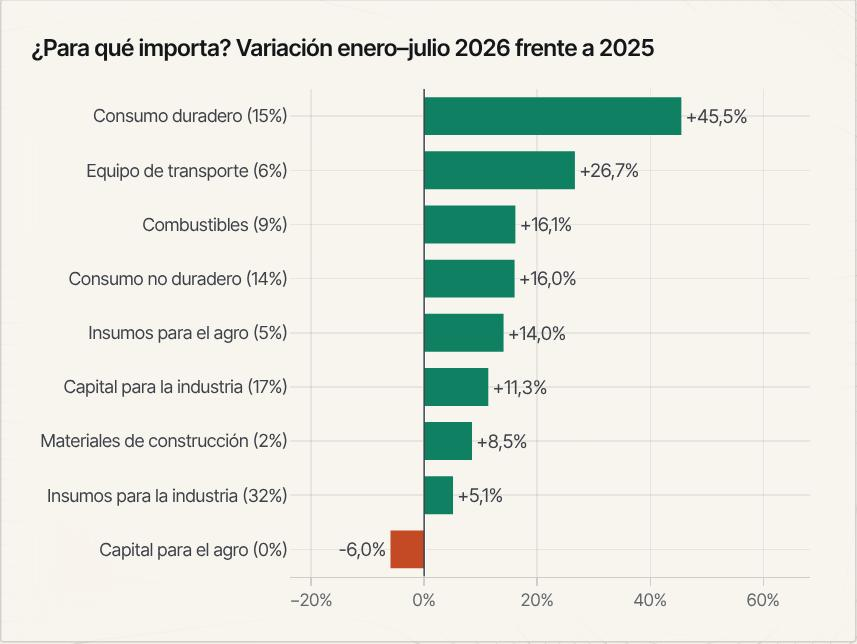
\includegraphics[width=\linewidth,height=0.42\textheight,keepaspectratio]{fig/g-impo-uso.jpg}\end{center}
\paragraph{Qué nos cuenta}
Muestra para qué compra bienes Colombia en el exterior y cuáles de esas compras crecen o caen en lo corrido del año frente al mismo periodo del año anterior. Usa la clasificación CUODE (Clasificación según Uso o Destino Económico), que separa las importaciones en bienes de consumo, materias primas e insumos, combustibles y bienes de capital. Así distingue si el movimiento de las importaciones viene del consumo de los hogares, de la producción o de la inversión.

\begin{leer}[Cómo se lee]
Barras horizontales, una por cada uno de los nueve subgrupos CUODE, ordenadas por su variación. El eje horizontal es la variación porcentual del valor CIF en dólares del periodo enero–último mes publicado frente al mismo periodo del año anterior; la línea vertical marca el cero. Verde: el grupo crece; naranja: cae. El número entre paréntesis junto al nombre es la participación del grupo en las importaciones totales del periodo, para ponderar su importancia.
\end{leer}

\paragraph{Por qué importa}
Las importaciones por uso son un termómetro adelantado de la demanda interna. Las compras de bienes de capital anticipan inversión en maquinaria y equipo; las materias primas para la industria acompañan la producción manufacturera; los bienes de consumo duradero (vehículos, electrodomésticos) reflejan la confianza y el crédito de los hogares. Para un inversionista permiten leer qué componente de la demanda empuja la economía.

\paragraph{Cómo interpretarlo}
\begin{itemize}
\item Una variación alta en un grupo con participación pequeña pesa poco en el total: combine siempre el signo y el tamaño de la barra con el número entre paréntesis.
\item El crecimiento de bienes de capital y equipo de transporte suele acompañar ciclos de inversión; el de consumo duradero, ciclos de crédito y confianza de los hogares.
\item Las variaciones están en dólares corrientes: una devaluación o una subida de precios internacionales cambia el valor sin que cambie la cantidad comprada.
\item Al ser año corrido, al comienzo del año pocos meses determinan el resultado; compare con la composición anual del gráfico vecino.
\end{itemize}
\begin{formulas}[Fórmulas]
\formula{Variación año corrido}{g\textsubscript{k} = (M\textsubscript{k,a} $\div$ M\textsubscript{k,a−1} − 1) $\times$ 100}{M\textsubscript{k,a} = importaciones CIF del grupo k de enero al último mes del año a; a−1 = mismo periodo del año anterior}
\formula{Participación (entre paréntesis)}{s\textsubscript{k} = M\textsubscript{k,a} $\div$ M\textsubscript{a} $\times$ 100}{M\textsubscript{a} = importaciones totales del periodo}
\end{formulas}
\begin{metodo}[Metodología]
Cuadro A13 del anexo de importaciones: clasificación CUODE (uso o destino económico), valor CIF del periodo enero–último mes frente al mismo periodo del año anterior. Entre paréntesis: participación en el total del periodo.
\par\smallskip{\small\textbf{Fuente:} DANE con registros de la DIAN: importaciones (anexos estadísticos)}
\end{metodo}

\subsection{Composición de las importaciones por uso}
\label{g:g-impo-estructura}
\begin{center}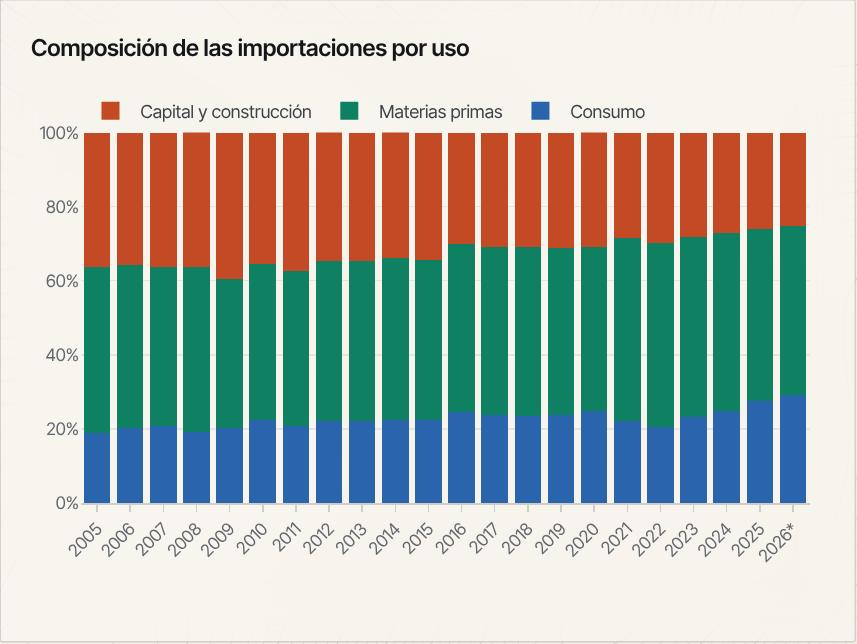
\includegraphics[width=\linewidth,height=0.42\textheight,keepaspectratio]{fig/g-impo-estructura.jpg}\end{center}
\paragraph{Qué nos cuenta}
Muestra cómo se reparten, año por año, las importaciones de Colombia entre los tres grandes grupos de la clasificación CUODE (uso o destino económico): bienes de consumo, materias primas e insumos, y bienes de capital y materiales de construcción. Permite ver si el país importa cada vez más para consumir, para producir o para invertir, y cómo cambia esa mezcla en recesiones y auges.

\begin{leer}[Cómo se lee]
Cada barra es un año y suma 100\%. Azul (abajo): bienes de consumo; verde: materias primas y productos intermedios, que incluyen combustibles; naranja (arriba): bienes de capital y materiales de construcción. Se excluyen las partidas «no clasificadas», de modo que las participaciones se calculan sobre la suma de los tres grupos. La serie empieza en 2005. El último año, marcado con asterisco (*), es el acumulado a la fecha y no un año completo.
\end{leer}

\paragraph{Por qué importa}
La estructura de las importaciones informa sobre el modelo de crecimiento: una mayor parte de bienes de capital se asocia a fases de inversión y ampliación de la capacidad productiva; una mayor parte de bienes de consumo, a fases impulsadas por el gasto de los hogares. Para un inversionista ayuda a evaluar la calidad del déficit comercial: no es lo mismo financiar maquinaria que bienes de consumo.

\paragraph{Cómo interpretarlo}
\begin{itemize}
\item Si la franja naranja se ensancha, el país dedica una mayor parte de sus compras externas a maquinaria, equipo y construcción.
\item Las participaciones dependen también de los precios: un encarecimiento del petróleo y de los insumos agranda la franja verde sin que cambie la cantidad importada.
\item El año parcial puede verse afectado por estacionalidad (compras concentradas en ciertos meses).
\item Para el detalle por subgrupo y su variación reciente, use el gráfico «¿Para qué importa?».
\end{itemize}
\begin{formulas}[Fórmulas]
\formula{Participación del grupo g en el año a}{s\textsubscript{g,a} = M\textsubscript{g,a} $\div$ (M\textsubscript{C,a} + M\textsubscript{MP,a} + M\textsubscript{K,a}) $\times$ 100}{M = importaciones CIF anuales; C = consumo; MP = materias primas; K = capital y construcción (sin «no clasificados»)}
\end{formulas}
\begin{metodo}[Metodología]
Participación de los tres grandes grupos CUODE en el valor CIF anual (sin «no clasificados»). El año en curso (*) es acumulado a la fecha.
\par\smallskip{\small\textbf{Fuente:} DANE con registros de la DIAN: importaciones (anexos estadísticos)}
\end{metodo}

\section{¿Con quién comercia?}

\subsection{¿A quién le vende? Parte de las exportaciones, 12 meses}
\label{g:g-destinos}
\begin{center}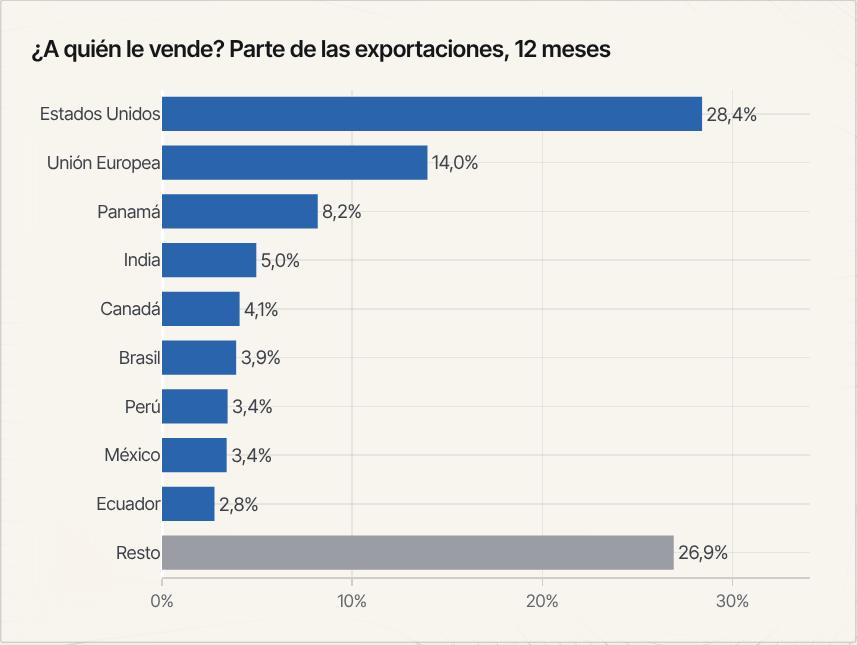
\includegraphics[width=\linewidth,height=0.42\textheight,keepaspectratio]{fig/g-destinos.jpg}\end{center}
\paragraph{Qué nos cuenta}
Muestra a quién le vende Colombia: qué parte de las exportaciones de los últimos 12 meses va a cada destino principal. Destaca el peso de Estados Unidos como primer comprador y el papel de la Unión Europea, Panamá, China y los vecinos latinoamericanos. Retrata la exposición del ingreso exportador a la demanda de cada socio y a sus políticas comerciales.

\begin{leer}[Cómo se lee]
Barras horizontales azules con los nueve destinos de mayor participación, ordenados de mayor a menor, y una barra gris al final, «Resto», que agrupa a todos los demás países (incluidos los destinos del anexo del DANE que no entran entre los nueve primeros). El eje horizontal y el número al final de cada barra son el porcentaje de las exportaciones FOB de los últimos 12 meses. La Unión Europea aparece como un solo destino, tal como la publica el DANE.
\end{leer}

\paragraph{Por qué importa}
La concentración de las ventas en pocos mercados expone al país a los ciclos económicos, las monedas y las decisiones arancelarias de esos socios. Un comprador dominante amplifica cualquier choque en su economía. Para un inversionista permite identificar qué economías extranjeras influyen más sobre los ingresos de los exportadores colombianos.

\paragraph{Cómo interpretarlo}
\begin{itemize}
\item Si sube la participación de un destino, ese mercado gana peso en la demanda externa del país; puede deberse a más ventas allí o a menos ventas en los demás.
\item La composición depende de los productos: los destinos del petróleo y el carbón cambian con los precios de esos bienes, lo que mueve las participaciones sin cambios de fondo en las relaciones comerciales.
\item Panamá incluye en parte mercancías en tránsito o reexportadas desde allí, por lo que no es necesariamente el destino final.
\item Para la evolución de la concentración en el tiempo, vea el gráfico de diversificación de destinos y productos.
\end{itemize}
\begin{formulas}[Fórmulas]
\formula{Participación del destino d}{s\textsubscript{d} = X12\textsubscript{d,t} $\div$ X12\textsubscript{t} $\times$ 100}{X12\textsubscript{d} = exportaciones FOB al destino d en 12 meses; X12 = exportaciones totales en 12 meses}
\formula{Resto}{s\textsubscript{Resto} = 100 − $\Sigma$\textsubscript{d$\in$top 9} s\textsubscript{d}}{agrupa todos los destinos fuera de los nueve principales}
\end{formulas}
\begin{metodo}[Metodología]
Anexo de exportaciones por principales destinos (valor FOB). Participación de la suma de 12 meses; «Resto» incluye los demás países.
\par\smallskip{\small\textbf{Fuente:} DANE con registros de la DIAN: exportaciones (anexos estadísticos)}
\end{metodo}

\subsection{¿A quién le compra? Parte de las importaciones, 12 meses}
\label{g:g-origenes}
\begin{center}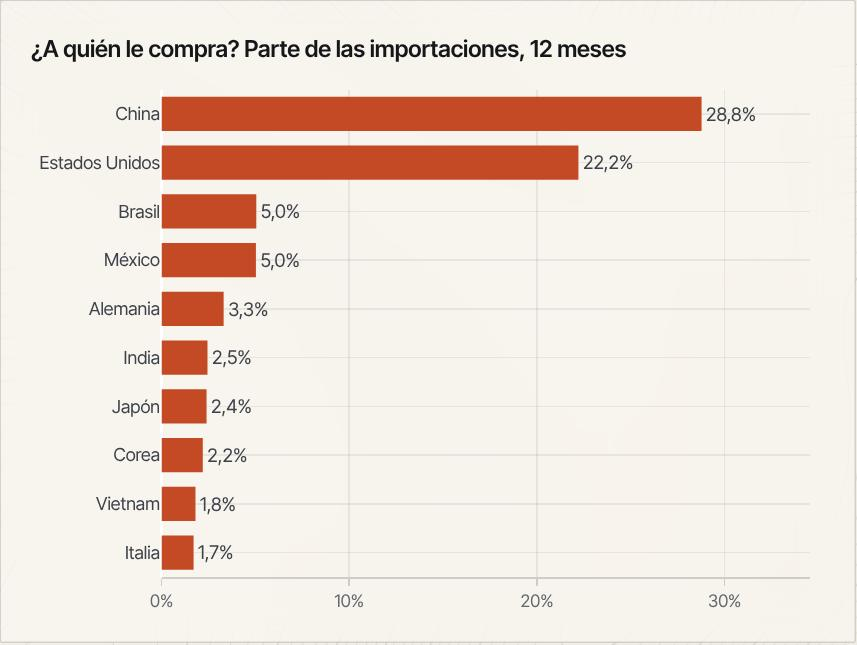
\includegraphics[width=\linewidth,height=0.42\textheight,keepaspectratio]{fig/g-origenes.jpg}\end{center}
\paragraph{Qué nos cuenta}
Muestra a quién le compra Colombia: qué parte de las importaciones de los últimos 12 meses proviene de cada uno de los diez países con mayor participación. Pone en evidencia que dos proveedores, Estados Unidos y China, concentran una parte muy grande de las compras externas, seguidos de socios regionales y europeos.

\begin{leer}[Cómo se lee]
Barras horizontales naranjas, ordenadas de mayor a menor, con los diez principales países de origen. El eje horizontal y el número al final de cada barra son el porcentaje de las importaciones CIF de los últimos 12 meses. El denominador son las importaciones totales publicadas por el DANE en esos 12 meses (sin las operaciones de zonas francas), de modo que los diez países no suman 100\%: la diferencia corresponde a los demás orígenes.
\end{leer}

\paragraph{Por qué importa}
El origen de las importaciones indica de qué economías depende el abastecimiento de bienes de consumo, insumos y maquinaria. Una alta dependencia de un proveedor expone los costos de las empresas y los precios al consumidor a su tasa de cambio, a sus cadenas de suministro y a cambios de política comercial. Para un inversionista ayuda a evaluar riesgos de abastecimiento y de costos importados.

\paragraph{Cómo interpretarlo}
\begin{itemize}
\item Un aumento de la participación de un país puede reflejar mayor competitividad de sus productos o cambios en lo que Colombia compra (por ejemplo, más combustibles o más electrónicos).
\item La evolución en el tiempo de las dos principales fuentes se ve en el gráfico de China, Estados Unidos y el resto.
\item El país de origen es donde se produjo la mercancía, no necesariamente desde donde se despachó.
\item Las cifras son en dólares CIF corrientes y las de los meses recientes son provisionales.
\end{itemize}
\begin{formulas}[Fórmulas]
\formula{Participación del país p}{s\textsubscript{p} = M12\textsubscript{p,t} $\div$ M12\textsuperscript{pub}\textsubscript{t} $\times$ 100}{M12\textsubscript{p} = importaciones CIF desde p en 12 meses; M12\textsuperscript{pub} = importaciones totales publicadas por el DANE en los mismos 12 meses}
\end{formulas}
\begin{metodo}[Metodología]
Anexo de importaciones por principales países de origen (valor CIF). Participación de la suma de 12 meses sobre las importaciones totales publicadas.
\par\smallskip{\small\textbf{Fuente:} DANE con registros de la DIAN: importaciones (anexos estadísticos)}
\end{metodo}

\section{¿Se vende más o se vende más caro?}

\subsection{Exportaciones: valor, precio y volumen (12 meses)}
\label{g:g-com-pq-expo}
\begin{center}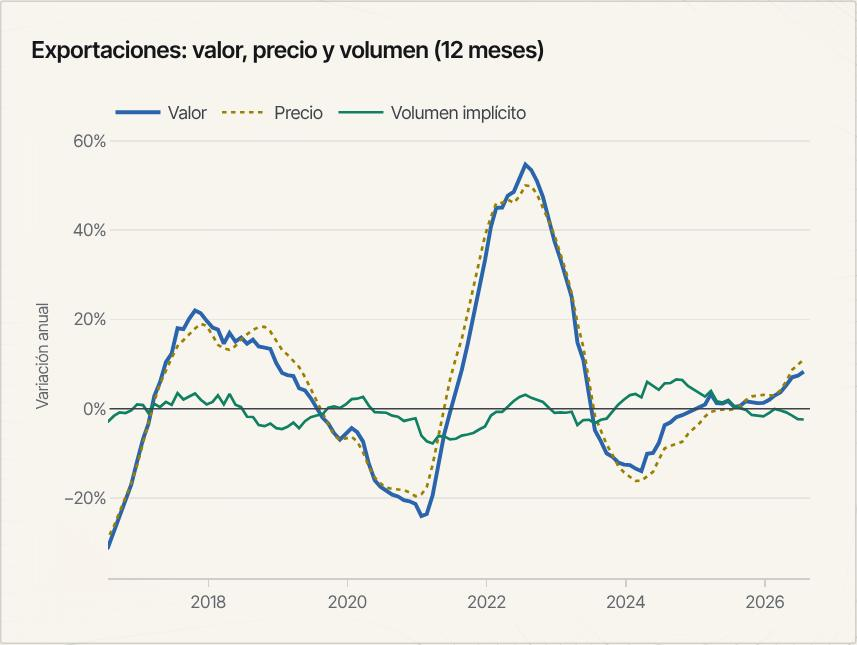
\includegraphics[width=\linewidth,height=0.42\textheight,keepaspectratio]{fig/g-com-pq-expo.jpg}\end{center}
\paragraph{Qué nos cuenta}
Descompone el crecimiento del valor de las exportaciones en dos partes: cuánto se debe a que los bienes se vendieron más caros o más baratos en dólares (precio) y cuánto a que se vendió más o menos cantidad (volumen). Responde a la pregunta de si Colombia exporta más o solo cobra más: en los auges y caídas del petróleo, casi todo el movimiento del valor suele venir del precio.

\begin{leer}[Cómo se lee]
Eje vertical en variación anual (\%), con una línea horizontal en cero. Línea azul gruesa: valor, variación anual de la suma de 12 meses de las exportaciones FOB del DANE. Línea amarilla punteada: precio, variación anual del promedio de 12 meses del índice de precios de exportación en dólares del Banco de la República. Línea verde: volumen implícito, lo que queda del valor después de descontar el precio. La serie empieza en 2005.
\end{leer}

\paragraph{Por qué importa}
Distinguir precio de volumen es clave para leer el comercio: una subida del valor por precios mejora el ingreso nacional y las cuentas fiscales, pero no indica que el aparato exportador produzca más; un aumento del volumen sí refleja más producción, empleo y capacidad. Para un inversionista ayuda a separar el efecto del ciclo de las materias primas del desempeño real de los sectores exportadores.

\paragraph{Cómo interpretarlo}
\begin{itemize}
\item Si la línea azul sube y la amarilla también mientras la verde está cerca de cero, el valor exportado crece por precios y no por cantidades.
\item Una línea verde positiva con precios en caída indica que se vende más cantidad aunque cada unidad valga menos.
\item El volumen implícito es un residuo: acumula cualquier diferencia de cobertura o de ponderación entre las cifras del DANE y el índice de precios, por lo que no es una medida directa de cantidades.
\item La relación entre este índice de precios y el de importaciones son los términos de intercambio, que aparecen en la tarjeta de medidas de la página.
\end{itemize}
\begin{formulas}[Fórmulas]
\formula{Valor}{v\textsubscript{t} = (X12\textsubscript{t} $\div$ X12\textsubscript{t−12} − 1) $\times$ 100}{X12 = suma de 12 meses de las exportaciones FOB}
\formula{Precio}{p\textsubscript{t} = ($\bar{\mathrm{P}}$12\textsubscript{t} $\div$ $\bar{\mathrm{P}}$12\textsubscript{t−12} − 1) $\times$ 100}{$\bar{\mathrm{P}}$12 = promedio de 12 meses del índice de precios de exportación en dólares}
\formula{Volumen implícito}{q\textsubscript{t} = [(1 + v\textsubscript{t}/100) $\div$ (1 + p\textsubscript{t}/100) − 1] $\times$ 100}{v y p en porcentaje; se cumple (1 + v) = (1 + p)(1 + q)}
\end{formulas}
\begin{metodo}[Metodología]
Valor: variación anual de la suma de 12 meses de las exportaciones FOB. Precio: variación anual del promedio de 12 meses del índice de precios de exportación en dólares. Volumen implícito = (1 + valor) / (1 + precio) − 1; es un residuo, no una medida directa de cantidades.
\par\smallskip{\small\textbf{Fuente:} DANE (exportaciones FOB) y Banco de la República (índice de precios de exportación en dólares)}
\end{metodo}

\subsection{Importaciones: valor, precio y volumen (12 meses)}
\label{g:g-com-pq-impo}
\begin{center}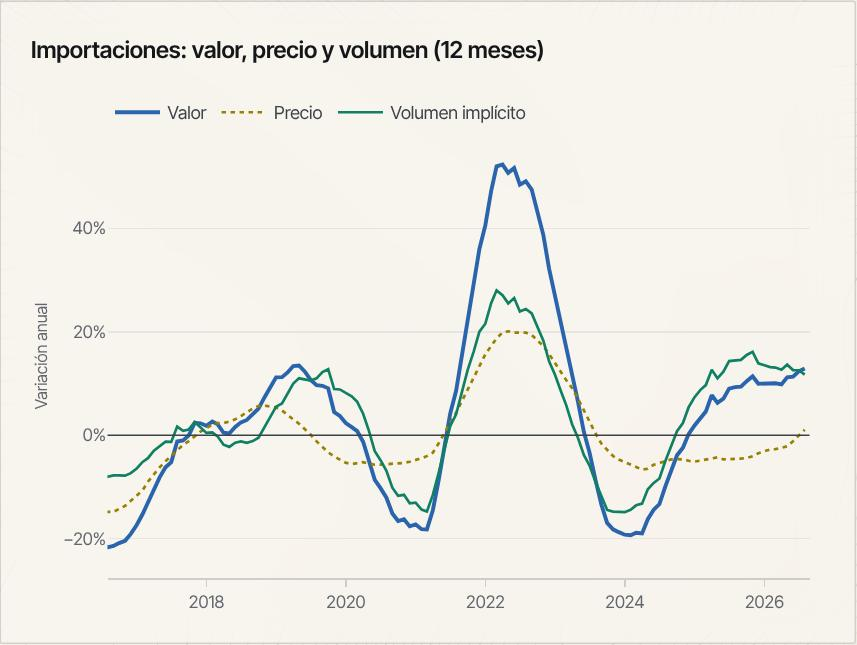
\includegraphics[width=\linewidth,height=0.42\textheight,keepaspectratio]{fig/g-com-pq-impo.jpg}\end{center}
\paragraph{Qué nos cuenta}
Aplica a las importaciones la misma descomposición que el gráfico de exportaciones: separa el crecimiento del valor importado en la parte que viene de precios en dólares y la que viene de la cantidad comprada. Permite saber si Colombia compra más bienes al exterior porque la demanda interna se expande o porque los bienes importados, como combustibles, insumos y maquinaria, se encarecieron.

\begin{leer}[Cómo se lee]
Eje vertical en variación anual (\%), con una línea horizontal en cero. Línea azul gruesa: valor, variación anual de la suma de 12 meses de las importaciones CIF totales del DANE. Línea amarilla punteada: precio, variación anual del promedio de 12 meses del índice de precios de importación en dólares del Banco de la República. Línea verde: volumen implícito, el residuo después de descontar el precio. La serie empieza en 2005.
\end{leer}

\paragraph{Por qué importa}
El volumen importado es un indicador cercano del gasto interno en bienes: crece con el consumo y la inversión y cae en las recesiones, a menudo con más fuerza que el PIB. El precio de las importaciones, por su parte, es un canal de la inflación externa hacia los costos de las empresas. Para un inversionista ayuda a leer el ciclo de la demanda interna y las presiones de costos importados.

\paragraph{Cómo interpretarlo}
\begin{itemize}
\item Una línea verde positiva y creciente indica que se están comprando más bienes al exterior, señal de demanda interna en expansión; una caída fuerte suele acompañar a las recesiones, como en 2020.
\item Si el valor sube sobre todo por la línea amarilla, el encarecimiento de lo importado explica el mayor gasto en dólares, no un mayor volumen.
\item Las importaciones están en dólares: el efecto de la tasa de cambio sobre la demanda se ve en el volumen con rezago, no en el precio en dólares.
\item Como en exportaciones, el volumen implícito es un residuo y no una medida directa de cantidades.
\end{itemize}
\begin{formulas}[Fórmulas]
\formula{Valor}{v\textsubscript{t} = (M12\textsubscript{t} $\div$ M12\textsubscript{t−12} − 1) $\times$ 100}{M12 = suma de 12 meses de las importaciones CIF totales}
\formula{Precio}{p\textsubscript{t} = ($\bar{\mathrm{P}}$12\textsubscript{t} $\div$ $\bar{\mathrm{P}}$12\textsubscript{t−12} − 1) $\times$ 100}{$\bar{\mathrm{P}}$12 = promedio de 12 meses del índice de precios de importación en dólares}
\formula{Volumen implícito}{q\textsubscript{t} = [(1 + v\textsubscript{t}/100) $\div$ (1 + p\textsubscript{t}/100) − 1] $\times$ 100}{v y p en porcentaje}
\end{formulas}
\begin{metodo}[Metodología]
Igual que el gráfico de exportaciones, con importaciones CIF totales y el índice de precios de importación. Volumen implícito = (1 + valor) / (1 + precio) − 1.
\par\smallskip{\small\textbf{Fuente:} DANE (importaciones CIF) y Banco de la República (índice de precios de importación en dólares)}
\end{metodo}

\section{Cómo ha cambiado lo que vende Colombia}

\subsection{Exportaciones por grupo de productos (12 meses)}
\label{g:g-com-canasta}
\begin{center}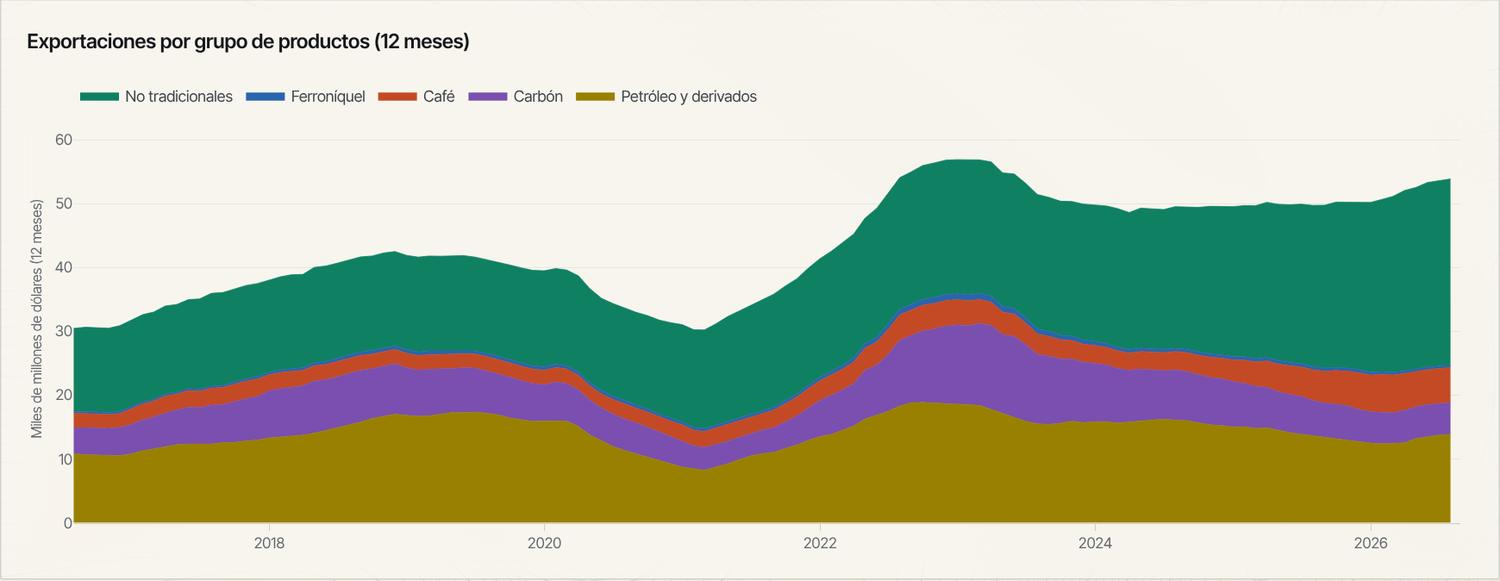
\includegraphics[width=\linewidth,height=0.42\textheight,keepaspectratio]{fig/g-com-canasta.jpg}\end{center}
\paragraph{Qué nos cuenta}
Muestra cómo ha cambiado en el tiempo lo que vende Colombia al exterior, separando las exportaciones en los cinco grupos del DANE. Cuenta la historia de la canasta exportadora: el auge del petróleo y el carbón durante la bonanza de las materias primas, su caída posterior y el crecimiento gradual de los productos no tradicionales, que con el tiempo se volvieron el grupo más grande.

\begin{leer}[Cómo se lee]
Áreas apiladas en miles de millones de dólares FOB; cada punto es la suma de los 12 meses que terminan en ese mes, desde mediados de los años noventa. De abajo hacia arriba: petróleo y derivados (amarillo), carbón (morado), café (naranja), ferroníquel (azul) y no tradicionales (verde). El grosor de cada franja es lo exportado por ese grupo y la altura total es el total exportado. Al pasar el cursor se ve el valor de cada grupo.
\end{leer}

\paragraph{Por qué importa}
La evolución de la canasta muestra si el país reduce su dependencia de los bienes minero-energéticos y si las exportaciones con mayor valor agregado ganan espacio. Esto incide en la estabilidad de los ingresos externos, en la sensibilidad de la tasa de cambio al petróleo y en el potencial de crecimiento de largo plazo. Para un inversionista ofrece una perspectiva histórica de la exposición a materias primas.

\paragraph{Cómo interpretarlo}
\begin{itemize}
\item Si la franja verde crece mientras las de petróleo y carbón se estrechan, la canasta se diversifica en valor.
\item Las franjas de petróleo y carbón cambian mucho con los precios internacionales: su encogimiento no siempre indica menor producción.
\item Compare con el gráfico de peso del petróleo y el carbón, que expresa la misma información como porcentaje del total.
\item Las cifras son en dólares corrientes: parte del crecimiento de largo plazo refleja inflación en dólares, no solo mayor volumen.
\end{itemize}
\begin{formulas}[Fórmulas]
\formula{Suma de 12 meses del grupo k}{X12\textsubscript{k,t} = $\Sigma$\textsubscript{j=0..11} X\textsubscript{k,t−j}}{k $\in$ \{petróleo, carbón, café, ferroníquel, no tradicionales\}; dólares FOB}
\formula{Altura total}{X12\textsubscript{t} = $\Sigma$\textsubscript{k} X12\textsubscript{k,t}}{exportaciones totales de 12 meses}
\end{formulas}
\begin{metodo}[Metodología]
Sumas móviles de 12 meses de las exportaciones FOB por grupo del DANE (café, carbón, petróleo y derivados, ferroníquel y no tradicionales), apiladas. La altura total es el total exportado en miles de millones de dólares.
\par\smallskip{\small\textbf{Fuente:} DANE con registros de la DIAN: exportaciones (anexos estadísticos)}
\end{metodo}

\section{La balanza con cada socio}

\subsection{Exportaciones menos importaciones con cada socio (12 meses)}
\label{g:g-com-bilateral}
\begin{center}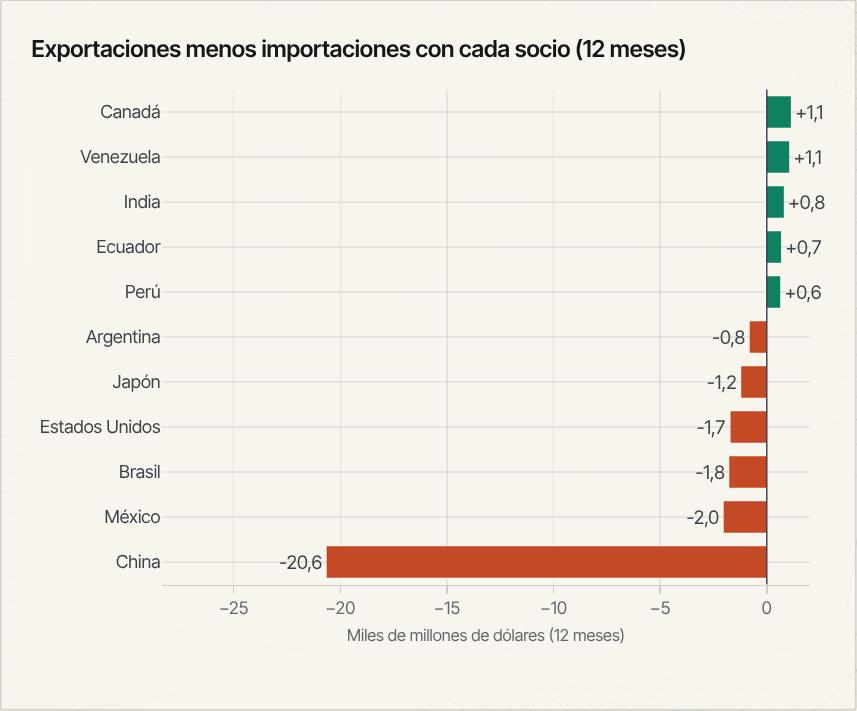
\includegraphics[width=\linewidth,height=0.42\textheight,keepaspectratio]{fig/g-com-bilateral.jpg}\end{center}
\paragraph{Qué nos cuenta}
Muestra con qué socios comerciales Colombia tiene superávit (les vende más de lo que les compra) y con cuáles tiene déficit, en los últimos 12 meses. Suele revelar un déficit grande con China, donde Colombia compra mucho y vende poco, y saldos más equilibrados o positivos con algunos vecinos latinoamericanos. Ayuda a entender de dónde viene el déficit comercial total.

\begin{leer}[Cómo se lee]
Barras horizontales en miles de millones de dólares, ordenadas del mayor déficit al mayor superávit. Cada barra es exportaciones FOB al país en 12 meses menos importaciones CIF desde ese país en los mismos 12 meses. Verde: superávit; naranja: déficit; la línea vertical marca el cero. El número junto a cada barra es el saldo con signo. Solo incluye socios individuales que aparecen a la vez en el anexo de destinos y en el de orígenes del DANE; la Unión Europea no está porque se publica como bloque.
\end{leer}

\paragraph{Por qué importa}
El saldo bilateral indica qué relaciones comerciales aportan dólares y cuáles los demandan, y qué tan expuesto está el país a la política comercial de cada socio. Para un inversionista ayuda a dimensionar el efecto de cambios arancelarios, de acuerdos comerciales o de choques en economías específicas sobre las cuentas externas de Colombia.

\paragraph{Cómo interpretarlo}
\begin{itemize}
\item Un déficit con un país no es por sí mismo un problema: puede reflejar que de allí vienen insumos y maquinaria que Colombia no produce.
\item Como las importaciones se valoran CIF (con flete y seguro) y las exportaciones FOB, todos los saldos aparecen algo más negativos que en la balanza de pagos.
\item El destino registrado de las exportaciones puede no ser el final (por ejemplo, ventas a través de Panamá), lo que afecta los saldos con algunos países.
\item La evolución de la participación de China y Estados Unidos en las compras se ve en el gráfico vecino.
\end{itemize}
\begin{formulas}[Fórmulas]
\formula{Saldo con el socio p}{B\textsubscript{p} = $\Sigma$\textsubscript{j=0..11} X\textsubscript{p,t−j} − $\Sigma$\textsubscript{j=0..11} M\textsubscript{p,t−j}}{X\textsubscript{p} = exportaciones FOB al país p; M\textsubscript{p} = importaciones CIF desde p; en miles de millones de dólares}
\end{formulas}
\begin{metodo}[Metodología]
Exportaciones FOB al país menos importaciones CIF desde el país, últimos 12 meses. Como las importaciones incluyen flete y seguro, el saldo es algo más negativo que en la balanza de pagos. Socios con información en los anexos de destinos y orígenes del DANE.
\par\smallskip{\small\textbf{Fuente:} DANE con registros de la DIAN: exportaciones e importaciones}
\end{metodo}

\subsection{¿De dónde vienen las importaciones? China, Estados Unidos y el resto}
\label{g:g-com-china}
\begin{center}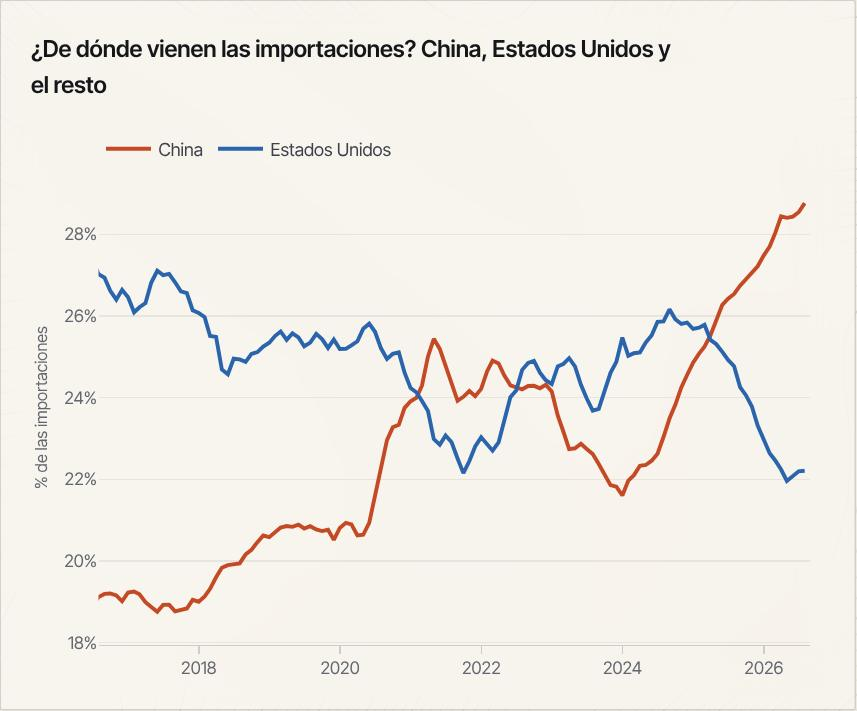
\includegraphics[width=\linewidth,height=0.42\textheight,keepaspectratio]{fig/g-com-china.jpg}\end{center}
\paragraph{Qué nos cuenta}
Muestra cómo ha cambiado el peso de los dos principales proveedores de Colombia: China y Estados Unidos. Cuenta una de las transformaciones más grandes del comercio colombiano en lo que va del siglo: el ascenso de China como fuente de importaciones de manufacturas, electrónicos, maquinaria y textiles, hasta disputarle el primer lugar a Estados Unidos, que históricamente fue el proveedor dominante.

\begin{leer}[Cómo se lee]
Dos líneas en porcentaje de las importaciones: naranja para China y azul para Estados Unidos. Cada punto divide las importaciones CIF desde ese país en los últimos 12 meses entre las importaciones totales publicadas por el DANE en los mismos 12 meses (sin zonas francas). La serie empieza cuando hay doce meses completos del anexo de países de origen del DANE. La diferencia hasta 100\% corresponde a todos los demás proveedores.
\end{leer}

\paragraph{Por qué importa}
La dependencia de pocos proveedores determina la exposición de los costos de las empresas y de los precios al consumidor a la tasa de cambio, la política industrial y las cadenas de suministro de esos países. El cruce entre China y Estados Unidos también tiene implicaciones para la política comercial y para los sectores colombianos que compiten con importaciones. Para un inversionista ayuda a evaluar riesgos geopolíticos y de abastecimiento.

\paragraph{Cómo interpretarlo}
\begin{itemize}
\item Si la línea naranja sube y la azul baja, China gana terreno como proveedor a costa de Estados Unidos; si ambas suben, las compras se concentran en esos dos países.
\item Las importaciones desde Estados Unidos incluyen muchos combustibles, cuyo peso cambia con el precio del petróleo, lo que mueve la línea azul sin cambios en las relaciones comerciales.
\item La participación es en valor: un abaratamiento de los bienes chinos puede reducir su línea aunque la cantidad comprada crezca.
\item Para el saldo comercial con cada uno de estos países, vea el gráfico de balanza con cada socio.
\end{itemize}
\begin{formulas}[Fórmulas]
\formula{Participación del país p}{s\textsubscript{p,t} = M12\textsubscript{p,t} $\div$ M12\textsuperscript{pub}\textsubscript{t} $\times$ 100}{M12\textsubscript{p} = importaciones CIF desde p (China o Estados Unidos) en 12 meses; M12\textsuperscript{pub} = importaciones totales publicadas en los mismos 12 meses}
\end{formulas}
\begin{metodo}[Metodología]
Importaciones CIF desde cada país (suma de 12 meses) sobre las importaciones totales publicadas por el DANE en el mismo periodo.
\par\smallskip{\small\textbf{Fuente:} DANE con registros de la DIAN: importaciones (anexos estadísticos)}
\end{metodo}

\section{Apertura y concentración}

\subsection{Apertura comercial de bienes (\% del PIB)}
\label{g:g-com-apertura}
\begin{center}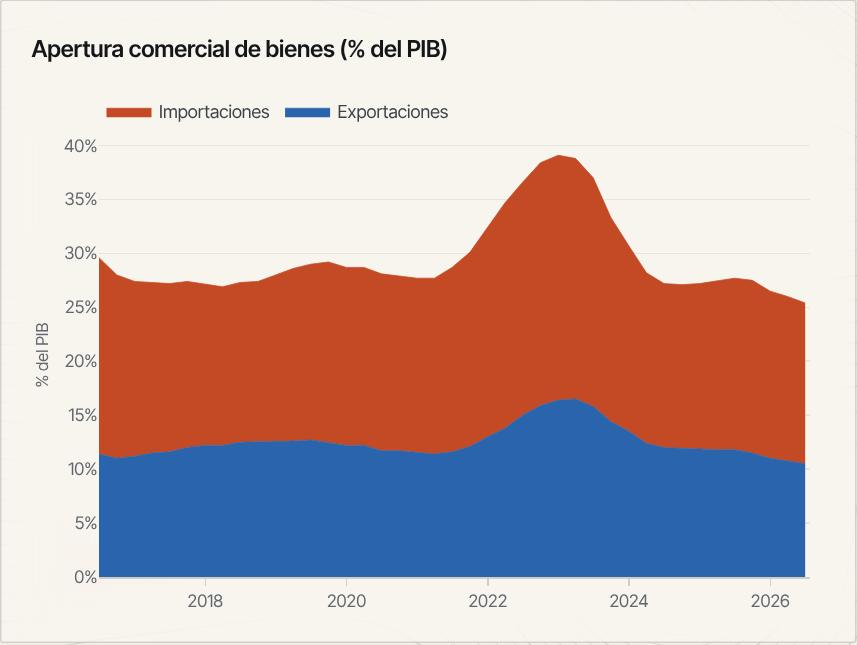
\includegraphics[width=\linewidth,height=0.42\textheight,keepaspectratio]{fig/g-com-apertura.jpg}\end{center}
\paragraph{Qué nos cuenta}
Mide qué tan abierta está la economía colombiana al comercio de bienes: cuánto suman las exportaciones y las importaciones en relación con el tamaño de la economía (el PIB). Colombia es una economía relativamente cerrada frente a otros países de tamaño similar; el indicador muestra si esa apertura aumenta o disminuye con el tiempo y cómo responde a los ciclos de precios de las materias primas y a la tasa de cambio.

\begin{leer}[Cómo se lee]
Áreas apiladas en porcentaje del PIB, trimestrales, desde 2005. Azul (abajo): exportaciones FOB de bienes; naranja (arriba): importaciones CIF. Ambas suman los últimos cuatro trimestres completos y se dividen por el PIB nominal de esos mismos cuatro trimestres, convertido a dólares con la TRM (tasa representativa del mercado, el tipo de cambio oficial peso-dólar) promedio de cada trimestre. La altura total es la apertura comercial de bienes.
\end{leer}

\paragraph{Por qué importa}
La apertura indica cuánto dependen la producción y el consumo del comercio exterior y, por tanto, qué tan expuesta está la economía a choques externos y a la tasa de cambio. Una mayor integración suele asociarse a más competencia, transferencia de tecnología y acceso a insumos. Para un inversionista ayuda a dimensionar el peso de los sectores transables y la sensibilidad de la economía al comercio mundial.

\paragraph{Cómo interpretarlo}
\begin{itemize}
\item Una subida puede venir de más comercio en dólares o de un PIB en dólares más pequeño: una fuerte devaluación del peso reduce el PIB en dólares y eleva la razón aunque el comercio no crezca.
\item Los auges de precios de las materias primas inflan las exportaciones en valor y, con ellas, la apertura.
\item Solo incluye bienes: no cuenta el comercio de servicios (turismo, transporte, servicios empresariales).
\item Las importaciones incluyen fletes y seguros (CIF), lo que eleva un poco la franja naranja frente a una medición FOB.
\end{itemize}
\begin{formulas}[Fórmulas]
\formula{PIB en dólares de 4 trimestres}{Y\$\textsubscript{t} = $\Sigma$\textsubscript{j=0..3} (PIB\textsubscript{t−j} $\div$ TRM\textsubscript{t−j})}{PIB = PIB nominal trimestral en pesos; TRM = promedio trimestral del tipo de cambio}
\formula{Apertura}{A\textsubscript{t} = (X4\textsubscript{t} + M4\textsubscript{t}) $\div$ Y\$\textsubscript{t} $\times$ 100}{X4 y M4 = exportaciones FOB e importaciones CIF de los últimos 4 trimestres completos, en dólares}
\end{formulas}
\begin{metodo}[Metodología]
Exportaciones FOB e importaciones CIF de los últimos 4 trimestres completos sobre el PIB nominal de los mismos 4 trimestres, convertido a dólares con la TRM promedio de cada trimestre. Áreas apiladas: la altura total es la apertura (X + M) / PIB.
\par\smallskip{\small\textbf{Fuente:} DANE: exportaciones, importaciones y PIB nominal; Banco de la República: TRM}
\end{metodo}

\subsection{Diversificación de destinos y productos}
\label{g:g-com-diversificacion}
\begin{center}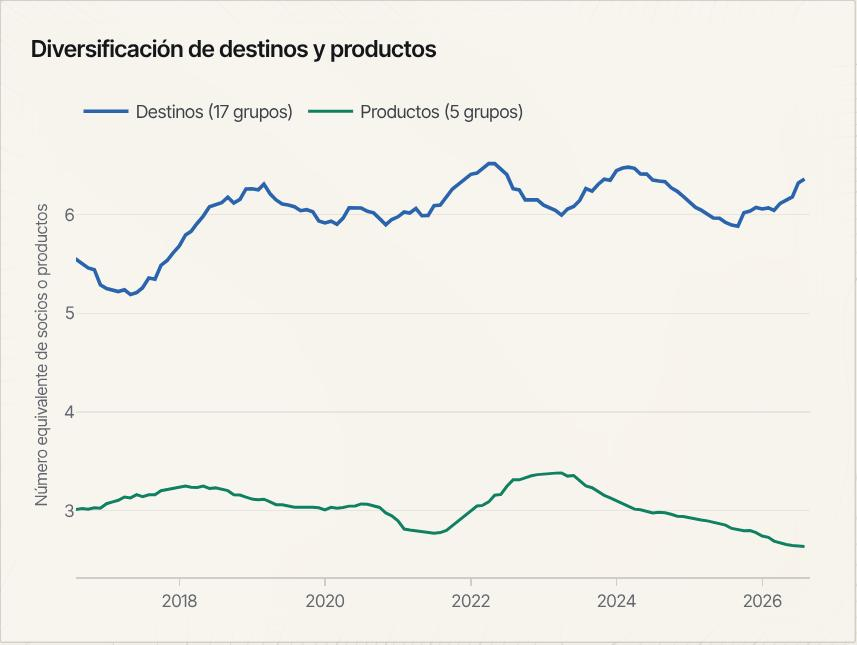
\includegraphics[width=\linewidth,height=0.42\textheight,keepaspectratio]{fig/g-com-diversificacion.jpg}\end{center}
\paragraph{Qué nos cuenta}
Mide qué tan repartidas están las exportaciones colombianas entre destinos y entre productos, con una medida muy usada en economía: el «número equivalente», que traduce la concentración a un número intuitivo de socios o productos de igual tamaño. Si Colombia vendiera lo mismo a cuatro destinos, el número sería 4; si vendiera todo a uno solo, sería 1. Muestra si la canasta y los mercados se diversifican o se concentran con el tiempo.

\begin{leer}[Cómo se lee]
Dos líneas desde 2005, con el eje en número equivalente. Línea azul: destinos, calculada sobre los 17 grupos del anexo de destinos del DANE (países individuales, la Unión Europea como bloque y «Resto»). Línea verde: productos, calculada sobre los cinco grupos del DANE (petróleo, carbón, café, ferroníquel y no tradicionales), por lo que su máximo posible es 5. Ambas usan participaciones de las sumas de 12 meses en dólares FOB.
\end{leer}

\paragraph{Por qué importa}
Una canasta y unos mercados diversificados hacen que los ingresos externos sean menos vulnerables a la caída de precios de un producto o a una recesión en un socio. La literatura sobre comercio y desarrollo asocia la diversificación con mayor estabilidad y con capacidades productivas más amplias. Para un inversionista, una mayor diversificación reduce la exposición de la economía a choques concentrados.

\paragraph{Cómo interpretarlo}
\begin{itemize}
\item Una línea que sube indica exportaciones más repartidas; una que baja, más concentración en pocos destinos o productos.
\item Durante auges del petróleo y el carbón, la línea de productos tiende a caer porque esos dos grupos dominan la canasta.
\item Como la Unión Europea y «Resto» se cuentan como un solo destino cada uno, el número de destinos subestima la diversificación real por países.
\item Con solo cinco grupos de productos, la medida es gruesa: no capta la diversificación dentro de los no tradicionales.
\end{itemize}
\begin{formulas}[Fórmulas]
\formula{Índice de Herfindahl}{H\textsubscript{t} = $\Sigma$\textsubscript{i} s\textsubscript{i,t}\textsuperscript{2}}{s\textsubscript{i} = participación (entre 0 y 1) del destino o producto i en las exportaciones de 12 meses}
\formula{Número equivalente}{N\textsubscript{t} = 1 $\div$ H\textsubscript{t}}{número de destinos o productos de igual tamaño que daría la misma concentración}
\end{formulas}
\begin{metodo}[Metodología]
Número equivalente = 1 / índice de Herfindahl (suma de participaciones al cuadrado), con sumas de 12 meses. Destinos: países del anexo de destinos del DANE (sin el total). Productos: los cinco grupos del DANE, por lo que su máximo posible es 5.
\par\smallskip{\small\textbf{Fuente:} DANE con registros de la DIAN: exportaciones (anexos estadísticos)}
\end{metodo}

\section*{Lecturas de la página}
\begin{itemize}\small
\item \textbf{Prebisch, R. (1950). The Economic Development of Latin America and its Principal Problems. Naciones Unidas, CEPAL.} Términos de intercambio y dependencia de las materias primas.
\item \textbf{Melitz, M. J. (2003). The Impact of Trade on Intra-Industry Reallocations and Aggregate Industry Productivity. Econometrica, 71(6), 1695–1725.} Por qué solo las empresas más productivas exportan.
\item \textbf{Hausmann, R., Hwang, J. y Rodrik, D. (2007). What You Export Matters. Journal of Economic Growth, 12(1), 1–25.} La composición de las exportaciones y el crecimiento.
\item \textbf{Hidalgo, C. A., Klinger, B., Barabási, A.-L. y Hausmann, R. (2007). The Product Space Conditions the Development of Nations. Science, 317(5837), 482–487.} Diversificación productiva y espacio de productos.
\item \textbf{DANE. Estadísticas de comercio internacional: exportaciones (FOB) e importaciones (CIF) con base en registros administrativos de la DIAN.} Fuente y definiciones de las cifras de esta página.
\end{itemize}
